\PassOptionsToPackage{enable-debug,check-declarations}{expl3}
\RequirePackage{pdfmanagement-testphase}
\DeclareDocumentMetadata {  }
\ExplSyntaxOn
\pdfmanagement_add:nnn{Catalog}{Lang}{(enUS)}
\ExplSyntaxOff

% xmp metadata for pdf
% Originally used \usepackage[a-2a]{pdfx}
% \usepackage{hyperxmp} replaced it
% \RequirePackage{pdfmanagement-testphase} replaced it

\documentclass[11pt,
  english,
  a4paper,
]{article}
\usepackage{sa4ss}
\usepackage{amsmath,amssymb,array}
\usepackage{booktabs}

% From tagged-template.latex
\usepackage{lmodern}
\usepackage{ifxetex,ifluatex}
\ifnum 0\ifxetex 1\fi\ifluatex 1\fi=0 % if pdftex
  \usepackage[T1]{fontenc}
  \usepackage[utf8]{inputenc}
  \usepackage{textcomp} % provide euro and other symbols
\else % if luatex or xetex
  \usepackage{unicode-math}
  \defaultfontfeatures{Scale=MatchLowercase}
  \defaultfontfeatures[\rmfamily]{Ligatures=TeX,Scale=1}
\fi

% Use upquote if available, for straight quotes in verbatim environments
\IfFileExists{upquote.sty}{\usepackage{upquote}}{}
\IfFileExists{microtype.sty}{% use microtype if available
  \usepackage[]{microtype}
  \UseMicrotypeSet[protrusion]{basicmath} % disable protrusion for tt fonts
}{}
\makeatletter
\@ifundefined{KOMAClassName}{% if non-KOMA class
  \IfFileExists{parskip.sty}{%
    \usepackage{parskip}
  }{% else
    \setlength{\parindent}{0pt}
    \setlength{\parskip}{6pt plus 2pt minus 1pt}}
}{% if KOMA class
  \KOMAoptions{parskip=half}}
\makeatother
\usepackage{xcolor}
\IfFileExists{xurl.sty}{\usepackage{xurl}}{} % add URL line breaks if available
\hypersetup{
  pdftitle={DRAFT The status of Vermilion Rockfish (Sebastes miniatus) and Sunset Rockfish (Sebastes crocotulus) in U.S. waters off the coast of California south of Pt. Conception in 2021},
  pdflang={en},
  hidelinks,
  pdfcreator={LaTeX via pandoc}}
\urlstyle{same} % disable monospaced font for URLs
\usepackage{color}
\usepackage{fancyvrb}
\newcommand{\VerbBar}{|}
\newcommand{\VERB}{\Verb[commandchars=\\\{\}]}
\DefineVerbatimEnvironment{Highlighting}{Verbatim}{commandchars=\\\{\}}
% Add ',fontsize=\small' for more characters per line
\usepackage{framed}
\definecolor{shadecolor}{RGB}{248,248,248}
\newenvironment{Shaded}{\begin{snugshade}}{\end{snugshade}}
\newcommand{\AlertTok}[1]{\textcolor[rgb]{0.94,0.16,0.16}{#1}}
\newcommand{\AnnotationTok}[1]{\textcolor[rgb]{0.56,0.35,0.01}{\textbf{\textit{#1}}}}
\newcommand{\AttributeTok}[1]{\textcolor[rgb]{0.77,0.63,0.00}{#1}}
\newcommand{\BaseNTok}[1]{\textcolor[rgb]{0.00,0.00,0.81}{#1}}
\newcommand{\BuiltInTok}[1]{#1}
\newcommand{\CharTok}[1]{\textcolor[rgb]{0.31,0.60,0.02}{#1}}
\newcommand{\CommentTok}[1]{\textcolor[rgb]{0.56,0.35,0.01}{\textit{#1}}}
\newcommand{\CommentVarTok}[1]{\textcolor[rgb]{0.56,0.35,0.01}{\textbf{\textit{#1}}}}
\newcommand{\ConstantTok}[1]{\textcolor[rgb]{0.00,0.00,0.00}{#1}}
\newcommand{\ControlFlowTok}[1]{\textcolor[rgb]{0.13,0.29,0.53}{\textbf{#1}}}
\newcommand{\DataTypeTok}[1]{\textcolor[rgb]{0.13,0.29,0.53}{#1}}
\newcommand{\DecValTok}[1]{\textcolor[rgb]{0.00,0.00,0.81}{#1}}
\newcommand{\DocumentationTok}[1]{\textcolor[rgb]{0.56,0.35,0.01}{\textbf{\textit{#1}}}}
\newcommand{\ErrorTok}[1]{\textcolor[rgb]{0.64,0.00,0.00}{\textbf{#1}}}
\newcommand{\ExtensionTok}[1]{#1}
\newcommand{\FloatTok}[1]{\textcolor[rgb]{0.00,0.00,0.81}{#1}}
\newcommand{\FunctionTok}[1]{\textcolor[rgb]{0.00,0.00,0.00}{#1}}
\newcommand{\ImportTok}[1]{#1}
\newcommand{\InformationTok}[1]{\textcolor[rgb]{0.56,0.35,0.01}{\textbf{\textit{#1}}}}
\newcommand{\KeywordTok}[1]{\textcolor[rgb]{0.13,0.29,0.53}{\textbf{#1}}}
\newcommand{\NormalTok}[1]{#1}
\newcommand{\OperatorTok}[1]{\textcolor[rgb]{0.81,0.36,0.00}{\textbf{#1}}}
\newcommand{\OtherTok}[1]{\textcolor[rgb]{0.56,0.35,0.01}{#1}}
\newcommand{\PreprocessorTok}[1]{\textcolor[rgb]{0.56,0.35,0.01}{\textit{#1}}}
\newcommand{\RegionMarkerTok}[1]{#1}
\newcommand{\SpecialCharTok}[1]{\textcolor[rgb]{0.00,0.00,0.00}{#1}}
\newcommand{\SpecialStringTok}[1]{\textcolor[rgb]{0.31,0.60,0.02}{#1}}
\newcommand{\StringTok}[1]{\textcolor[rgb]{0.31,0.60,0.02}{#1}}
\newcommand{\VariableTok}[1]{\textcolor[rgb]{0.00,0.00,0.00}{#1}}
\newcommand{\VerbatimStringTok}[1]{\textcolor[rgb]{0.31,0.60,0.02}{#1}}
\newcommand{\WarningTok}[1]{\textcolor[rgb]{0.56,0.35,0.01}{\textbf{\textit{#1}}}}
\usepackage{longtable}
% Correct order of tables after \paragraph or \subparagraph
\usepackage{etoolbox}
\makeatletter
\patchcmd\longtable{\par}{\if@noskipsec\mbox{}\fi\par}{}{}
\makeatother
% Allow footnotes in longtable head/foot
\IfFileExists{footnotehyper.sty}{\usepackage{footnotehyper}}{\usepackage{footnote}}
\makesavenoteenv{longtable}
\usepackage{graphicx}
\makeatletter
\def\maxwidth{\ifdim\Gin@nat@width>\linewidth\linewidth\else\Gin@nat@width\fi}
\def\maxheight{\ifdim\Gin@nat@height>\textheight\textheight\else\Gin@nat@height\fi}
\makeatother
% Scale images if necessary, so that they will not overflow the page
% margins by default, and it is still possible to overwrite the defaults
% using explicit options in \includegraphics[width, height, ...]{}
\setkeys{Gin}{width=\maxwidth,height=\maxheight,keepaspectratio}
% Set default figure placement to htbp
\makeatletter
\def\fps@figure{htbp}
\makeatother
\setlength{\emergencystretch}{3em} % prevent overfull lines
\providecommand{\tightlist}{%
  \setlength{\itemsep}{0pt}\setlength{\parskip}{0pt}}
\setcounter{secnumdepth}{5}
\usepackage{booktabs}
\usepackage{longtable}
\usepackage{array}
\usepackage{multirow}
\usepackage{wrapfig}
\usepackage{float}
\usepackage{colortbl}
\usepackage{pdflscape}
\usepackage{tabu}
\usepackage{threeparttable}
\usepackage[normalem]{ulem}
\usepackage{makecell}
\usepackage{xcolor}
\usepackage{placeins}
\ifxetex
  % Load polyglossia as late as possible: uses bidi with RTL langages (e.g. Hebrew, Arabic)
  \usepackage{polyglossia}
  \setmainlanguage[]{english}
\else
  \usepackage[shorthands=off,main=english]{babel}
\fi

%Define cslreferences environment, required by pandoc 2.8
%https://github.com/rstudio/rmarkdown/issues/1649
\newlength{\csllabelwidth}
\setlength{\csllabelwidth}{3em}
\newlength{\cslhangindent}
\setlength{\cslhangindent}{1.5em}
% for Pandoc 2.8 to 2.10.1
\newenvironment{cslreferences}%
  {}%
  {\par}
% For Pandoc 2.11+
\newenvironment{CSLReferences}[2] % #1 hanging-ident, #2 entry spacing
 {% don't indent paragraphs
  \setlength{\parindent}{0pt}
  % turn on hanging indent if param 1 is 1
  \ifodd #1 \everypar{\setlength{\hangindent}{\cslhangindent}}\ignorespaces\fi
  % set entry spacing
  \ifnum #2 > 0
  \setlength{\parskip}{#2\baselineskip}
  \fi
 }%
 {}
\usepackage{calc}  % for \widthof, \maxof in minipage
\newcommand{\CSLBlock}[1]{#1\hfill\break}
\newcommand{\CSLLeftMargin}[1]{\parbox[t]{\csllabelwidth}{#1}}
\newcommand{\CSLRightInline}[1]{\parbox[t]{\linewidth - \csllabelwidth}{#1}\break}
\newcommand{\CSLIndent}[1]{\hspace{\cslhangindent}#1}


\providecommand{\tightlist}{%
  \setlength{\itemsep}{0pt}\setlength{\parskip}{0pt}}

\usepackage{booktabs}
\usepackage{longtable}
\usepackage{array}
\usepackage{multirow}
\usepackage{wrapfig}
\usepackage{float}
\usepackage{colortbl}
\usepackage{pdflscape}
\usepackage{tabu}
\usepackage{threeparttable}
\usepackage[normalem]{ulem}
\usepackage{makecell}
\usepackage{xcolor}
\usepackage{placeins}
\date{}
\newcommand{\trTitle}{DRAFT The status of Vermilion Rockfish (\emph{Sebastes miniatus}) and Sunset Rockfish (\emph{Sebastes crocotulus}) in U.S. waters off the coast of California south of Pt. Conception in 2021}
\newcommand{\trYear}{2021}
\newcommand{\trMonth}{July}
\newcommand{\trAuthsLong}{truetruetruetruetrue}
\newcommand{\trAuthsBack}{Dick, E.J., M.H. Monk, T.L. Rogers, J.C. Field, E.M. Saas}
\newcommand{\trCitation}{
\begin{hangparas}{1em}{1}
\trAuthsBack{}. \trYear{}. \trTitle{}. Pacific Fisheries Management Council, Portland, Oregon. \pageref{LastPage}{}\,p.
\end{hangparas}}

\AtBeginDocument{\tagstructbegin{tag=Document}}
\AtEndDocument{\tagstructend}
\pretocmd{\maketitle}{\tagstructbegin{tag=H1}\tagmcbegin{tag=H1}}{}{}
\apptocmd{\maketitle}{\tagmcend\tagstructend}{}{}

\begin{document}

%%%%% Frontmatter %%%%%

% Footnote symbols in front matter
\renewcommand*{\thefootnote}{\fnsymbol{footnote}}

\small
\thispagestyle{empty}
\pagenumbering{roman}
\noindent
\begin{center}
\title{DRAFT The status of Vermilion Rockfish (\emph{Sebastes miniatus}) and Sunset Rockfish (\emph{Sebastes crocotulus}) in U.S. waters off the coast of California south of Pt. Conception in 2021}
% \textnormal{\MakeTextUppercase{\trTitle{}}}
\vspace{1.5cm}
{\Large\textbf\newline{DRAFT The status of Vermilion Rockfish (\emph{Sebastes miniatus}) and Sunset Rockfish (\emph{Sebastes crocotulus}) in U.S. waters off the coast of California south of Pt. Conception in 2021}}
\vfill
by\\
E. J. Dick\textsuperscript{1}\\
Melissa H. Monk\textsuperscript{1}\\
Tanya L. Rogers\textsuperscript{1}\\
John C. Field\textsuperscript{1}\\
Emma M. Saas\textsuperscript{1}\vfill
\textsuperscript{1}Southwest Fisheries Science Center, U.S. Department of Commerce, National Oceanic and Atmospheric Administration, National Marine Fisheries Service, 110 McAllister Way, Santa Cruz, California 95060\vfill
\trMonth{} \trYear{}
\end{center}
\clearpage

% Fourth page: Colophon
\thispagestyle{empty}
\vspace*{\fill}
\begin{center}
\copyright{} Pacific Fisheries Management Council, \trYear{}\\
\end{center}
\par
\bigskip
\noindent
Correct citation for this publication:
\bigskip
\par
\trCitation{}
\clearpage

% Add TOC to pdf bookmarks (clickable pdf)
\pdfbookmark[1]{\contentsname}{toc}

% Table of contents page, lists of figures and tables
\tableofcontents\clearpage
\label{TRlastRoman}
\clearpage

% Table of contents
\newpage
\thispagestyle{empty} % to remove page number

% Settings for the main document
\pagenumbering{arabic}  % Regular page numbers
\pagestyle{plain}  % No page number on first page of main document, use 'empty'
\renewcommand*{\thefootnote}{\arabic{footnote}}  % Back to numeric footnotes
\setcounter{footnote}{0}  % And start at 1
\renewcommand{\headrulewidth}{0.5pt}
\renewcommand{\footrulewidth}{0.5pt}
%\pagestyle{fancy}\fancyhead[c]{Draft: Do not cite or circulate}

\newcommand{\lt}{\ensuremath <}
\newcommand{\gt}{\ensuremath >}

\newcommand\CapeM{$40^\circ 10^\prime N$}
\newcommand\PtC{$34^\circ 27^\prime N$}
\newcommand\CAOR{$42^\circ 00^\prime N$}

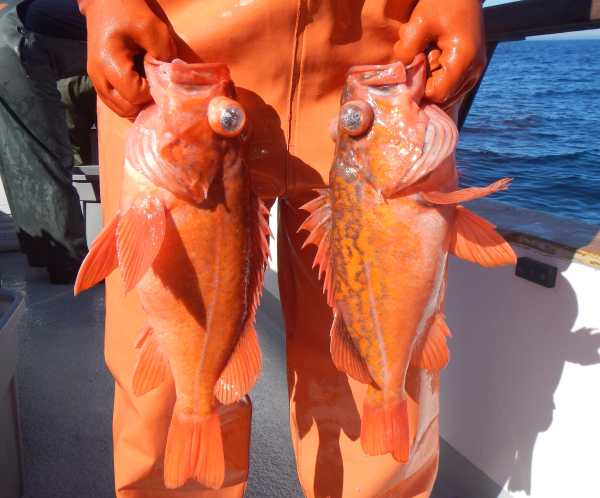
\includegraphics{cover_photo.png} Two fish of the vermilion/sunset cryptic species pair. Confirmation of species can only be determined via genetic analysis and species identification of these two fish caught in the Santa Barbara channel at approximately 250 ft depth is unknown. Photo courtesy of Sabrina Beyer.

\printnoidxglossary[sort=word]

\newpage

\pagebreak
\pagenumbering{roman}
\setcounter{page}{1}

\renewcommand{\thetable}{\roman{table}}
\renewcommand{\thefigure}{\roman{figure}}

\setlength\parskip{0.5em plus 0.1em minus 0.2em}

\newpage

\tagstructbegin{tag=H1}\tagmcbegin{tag=H1}

\hypertarget{executive-summary}{%
\section*{Executive Summary}\label{executive-summary}}
\addcontentsline{toc}{section}{Executive Summary}

\leavevmode\tagmcend\tagstructend

To be completed after the STAR panel.

\tagstructbegin{tag=H2}\tagmcbegin{tag=H2}

\hypertarget{stock}{%
\subsection*{Stock}\label{stock}}
\addcontentsline{toc}{subsection}{Stock}

\leavevmode\tagmcend\tagstructend

This assessment reports the status of the vermlion rockfish (\emph{Sebastes miniatus}) and sunset rockfish (\emph{Sebastes crocotulus}) complex (referred to as vermilion throughout), resource in U.S. waters off the coast of California north of Point Conception ({\tagstructbegin{tag=Formula}\tagmcbegin{tag=Formula}\(34^\circ 27^\prime\)\leavevmode\tagmcend\tagstructend} N. latitude) using data through 2020.

\tagstructbegin{tag=H2}\tagmcbegin{tag=H2}

\hypertarget{landings}{%
\subsection*{Landings}\label{landings}}
\addcontentsline{toc}{subsection}{Landings}

\leavevmode\tagmcend\tagstructend

Replace text.

\tagstructbegin{tag=H2}\tagmcbegin{tag=H2}

\hypertarget{data-and-assessment}{%
\subsection*{Data and Assessment}\label{data-and-assessment}}
\addcontentsline{toc}{subsection}{Data and Assessment}

\leavevmode\tagmcend\tagstructend

Replace text.

\tagstructbegin{tag=H2}\tagmcbegin{tag=H2}

\hypertarget{stock-biomass}{%
\subsection*{Stock Biomass}\label{stock-biomass}}
\addcontentsline{toc}{subsection}{Stock Biomass}

\leavevmode\tagmcend\tagstructend

Replace text.

\tagstructbegin{tag=H2}\tagmcbegin{tag=H2}

\hypertarget{recruitment}{%
\subsection*{Recruitment}\label{recruitment}}
\addcontentsline{toc}{subsection}{Recruitment}

\leavevmode\tagmcend\tagstructend

Replace text.

\tagstructbegin{tag=H2}\tagmcbegin{tag=H2}

\hypertarget{exploitation-status}{%
\subsection*{Exploitation Status}\label{exploitation-status}}
\addcontentsline{toc}{subsection}{Exploitation Status}

\leavevmode\tagmcend\tagstructend

Replace text.

\tagstructbegin{tag=H2}\tagmcbegin{tag=H2}

\hypertarget{reference-points}{%
\subsection*{Reference Points}\label{reference-points}}
\addcontentsline{toc}{subsection}{Reference Points}

\leavevmode\tagmcend\tagstructend

Replace text.

\tagstructbegin{tag=H2}\tagmcbegin{tag=H2}

\hypertarget{management-performance}{%
\subsection*{Management Performance}\label{management-performance}}
\addcontentsline{toc}{subsection}{Management Performance}

\leavevmode\tagmcend\tagstructend

Replace text.

\tagstructbegin{tag=H2}\tagmcbegin{tag=H2}

\hypertarget{unresolved-problems-and-major-uncertainties}{%
\subsection*{Unresolved Problems and Major Uncertainties}\label{unresolved-problems-and-major-uncertainties}}
\addcontentsline{toc}{subsection}{Unresolved Problems and Major Uncertainties}

\leavevmode\tagmcend\tagstructend

Replace text.

\tagstructbegin{tag=H2}\tagmcbegin{tag=H2}

\hypertarget{decision-table}{%
\subsection*{Decision Table}\label{decision-table}}
\addcontentsline{toc}{subsection}{Decision Table}

\leavevmode\tagmcend\tagstructend

Replace text.

\tagstructbegin{tag=H2}\tagmcbegin{tag=H2}

\hypertarget{research-and-data-needs}{%
\subsection*{Research and Data Needs}\label{research-and-data-needs}}
\addcontentsline{toc}{subsection}{Research and Data Needs}

\leavevmode\tagmcend\tagstructend

Replace text.

\pagebreak
\setlength{\parskip}{5mm plus1mm minus1mm}
\pagenumbering{arabic}
\setcounter{page}{1}
\renewcommand{\thefigure}{\arabic{figure}}
\renewcommand{\thetable}{\arabic{table}}
\setcounter{table}{0}
\setcounter{figure}{0}

\tagstructbegin{tag=H1}\tagmcbegin{tag=H1}

\hypertarget{introduction}{%
\section{Introduction}\label{introduction}}

\leavevmode\tagmcend\tagstructend

Note to readers: Text in section is the same in both California vermilion rockfish assessment documents.

\tagstructbegin{tag=H2}\tagmcbegin{tag=H2}

\hypertarget{basic-information-and-life-history}{%
\subsection{Basic Information and Life History}\label{basic-information-and-life-history}}

\leavevmode\tagmcend\tagstructend

Vermilion rockfish range from Prince William Sound, Alaska, to central Baja California at depths of 6 m to 436 m {\tagstructbegin{tag=Reference}\tagmcbegin{tag=Reference}(M. Love, Yoklavich, and Thorsteinson 2002)\leavevmode\tagmcend\tagstructend}. However, they are most commonly found from central Oregon to Punta Baja, Mexico {\tagstructbegin{tag=Reference}\tagmcbegin{tag=Reference}(J. R. Hyde and Vetter 2009)\leavevmode\tagmcend\tagstructend} at depths of 50 m to 150 m {\tagstructbegin{tag=Reference}\tagmcbegin{tag=Reference}(J. R. Hyde and Vetter 2009)\leavevmode\tagmcend\tagstructend}. Hyde and Vetter {\tagstructbegin{tag=Reference}\tagmcbegin{tag=Reference}(2009)\leavevmode\tagmcend\tagstructend} describe vermilion rockfish as residents of shallower depths (\textless100 m) than sunset rockfish. Adult fish tend to cluster on high relief rocky outcrops {\tagstructbegin{tag=Reference}\tagmcbegin{tag=Reference}(M. Love, Yoklavich, and Thorsteinson 2002)\leavevmode\tagmcend\tagstructend} and kelp forests {\tagstructbegin{tag=Reference}\tagmcbegin{tag=Reference}(J. R. Hyde and Vetter 2009)\leavevmode\tagmcend\tagstructend}. North of Point Conception, some adults are shallower, living in caves and cracks {\tagstructbegin{tag=Reference}\tagmcbegin{tag=Reference}(M. Love, Yoklavich, and Thorsteinson 2002)\leavevmode\tagmcend\tagstructend}. Vermilion rockfish have shown high site fidelity {\tagstructbegin{tag=Reference}\tagmcbegin{tag=Reference}(Hannah and Rankin 2011 (only tagged 1 vermilion); Lea, McAllister, and VenTresca 1999)\leavevmode\tagmcend\tagstructend}, and low average larval dispersal distance {\tagstructbegin{tag=Reference}\tagmcbegin{tag=Reference}(J. R. Hyde and Vetter 2009)\leavevmode\tagmcend\tagstructend}. Lowe et al.~(2009) {\tagstructbegin{tag=Reference}\tagmcbegin{tag=Reference}(2009)\leavevmode\tagmcend\tagstructend} suggested vermilion rockfish to have a lower site fidelity than previously believed, but they acknowledged that their observations of movements to different depths may have been due to the reality of a shallower species and a deeper species. Approximate lifespan for vermilion rockfish is 60 years, with females living longer and growing larger than their male counterparts. 50\% are mature at 5 years and about 37 cm, with males probably maturing at shorter lengths than females {\tagstructbegin{tag=Reference}\tagmcbegin{tag=Reference}(M. Love, Yoklavich, and Thorsteinson 2002)\leavevmode\tagmcend\tagstructend}.

Vermilion rockfish are viviparous, and release 63,000 to 2,600,000 eggs per season. In southern California, vermilion rockfish larvae are released between July and March. In central and northern California, this release occurs in September, December, and April-June {\tagstructbegin{tag=Reference}\tagmcbegin{tag=Reference}(M. Love, Yoklavich, and Thorsteinson 2002)\leavevmode\tagmcend\tagstructend}. Larval release in fall and winter is not common among other rockfish species. Hyde and Vetter {\tagstructbegin{tag=Reference}\tagmcbegin{tag=Reference}(2009)\leavevmode\tagmcend\tagstructend} suggest that low larval dispersal may be due to weak poleward flow of nearshore waters corresponding with peak vermilion larval release.

Young-of-the-year vermilion rockfish settle out of the plankton during two recruitment periods per year, first from February to April and a second from August to October, and settlement has been observed in May off southern California {\tagstructbegin{tag=Reference}\tagmcbegin{tag=Reference}(M. Love, Yoklavich, and Thorsteinson 2002)\leavevmode\tagmcend\tagstructend}. Larvae measure about 4.3 mm. Both young-of-the-year vermilion and sunset rockfish are mottled brown with areas of black, and older juveniles turn a mottled orange or red color {\tagstructbegin{tag=Reference}\tagmcbegin{tag=Reference}(M. S. Love et al. 2012)\leavevmode\tagmcend\tagstructend}. Juvenile fish are found individually from 6 m to 36 m, living near sand and structures. After two months, juveniles travel deeper and live on low relief rocky outcrops and other structures {\tagstructbegin{tag=Reference}\tagmcbegin{tag=Reference}(M. Love, Yoklavich, and Thorsteinson 2002)\leavevmode\tagmcend\tagstructend}.

Adult vermilion rockfish predominantly eat smaller fish, though sometimes they pursue euphausiids and other various macroplankton {\tagstructbegin{tag=Reference}\tagmcbegin{tag=Reference}(Phillips 1964)\leavevmode\tagmcend\tagstructend}. Love {\tagstructbegin{tag=Reference}\tagmcbegin{tag=Reference}(2002)\leavevmode\tagmcend\tagstructend} noted their diet to include octopus, salps, shrimps, and pelagic red crabs.

\emph{Population Structure and Complex Assessment Considerations}

This assessment represents the cryptic species pair vermilion rockfish (\emph{Sebastes miniatus}) and sunset rockfish (\emph{Sebastes crocotulus}). Hyde {\tagstructbegin{tag=Reference}\tagmcbegin{tag=Reference}(2007)\leavevmode\tagmcend\tagstructend} found seven mirochondrial and two nuclear genes analysis suggested three species within the subgenus \emph{Rosicola}. Hyde et al.~ {\tagstructbegin{tag=Reference}\tagmcbegin{tag=Reference}(2008)\leavevmode\tagmcend\tagstructend} described sunset rockfish as a distinct species noting depth separation of the adult populations of the two species using nine microsatellite loci. Sunset rockfish is distributed at depths greater than 50 fm (100 m) and are predominantly located south of Point Conception ($34^\circ 27^\prime N$). Hyde and Budrick identified speciation using mtDNA assay and size microsatelite loci, respectively. The mtDNA analyses proved to be subject to introgression and mis-specification of sunset rockfish from mating between the two species post-divergence. Additional population clusters of vermilion were found north of Point Conception, but neither study detected population structure between Half Moon Bay, California and Brookings, Oregon {\tagstructbegin{tag=Reference}\tagmcbegin{tag=Reference}(J. R. Hyde and Vetter 2009; Budrick 2016)\leavevmode\tagmcend\tagstructend}.

Vermilion and sunset rockfishes are morphologically very similar, with the most commonly cited differentiating feature being color. Hyde {\tagstructbegin{tag=Reference}\tagmcbegin{tag=Reference}(2009)\leavevmode\tagmcend\tagstructend} noted differences in three of six morphological parameters examined, but none of them can readily be used for field identification.

In all historical and current recreational and commercial catches, sunset and vermilion rockfish are both recorded as vermilion rockfish. Future studies, such as the one described below will provide data needed to compare biological parameters between the two species as well as habitats.

\emph{Ongoing Population Structure Research (Provided by John Harms, NWFSC)}

A group of researchers from the NWFSC and SWFSC is collaborating on a project to genotype tissue specimens collected from the vermilion and sunset rockfish cryptic pair captured during the West Coast Groundfish Bottom Trawl Survey and the Southern CA Shelf Rockfish Hook and Line Survey for the years 2004 - 2019. Funding for this project was obtained through the Saltonstall-Kennedy program for FY 2020 through a proposal led by representatives from Pacific States Marine Fisheries Commission and the commercial passenger fishing vessel industry in southern California.

After combining with specimens obtained through other collection efforts along the West Coast, approximately 25,000 tissue specimens will be analyzed. Some earlier efforts to separate this cryptic pair to species used mitochondrial DNA (mtDNA) markers. However, due to a one-way mitochondrial introgression from the vermilion genome into the sunset genome, a portion of the sunset rockfish population contains mitochondrial DNA sequences consistent with vermilion rockfish resulting in incorrect species assignments for these introgressed individuals during the prior research project. The current research has identified a robust suite of genetic markers within the nuclear genomes of the two species that definitively separates vermilion and sunset rockfish (including introgressed sunset rockfish), canary rockfish, first generation vermilion-sunset hybrids, and identifies emerging patterns of intraspecific stock structure within the two sister species.

Once the collected specimens have been genotyped, any species-specific differences in spatial and depth distribution, size composition, weight-length relationships, and other biological characteristics will be identified. Using previously collected otoliths and ovaries, the demographics of the two species including age and growth and reproductive biology parameters such as length and age at 50\% maturity and the prevalence of skip spawning will be explored and compared. These new genotyping results will be combined with data from the prior mtDNA work to evaluate whether introgressed sunset rockfish represent a biologically intermediate subform of the species complex. The effort also proposes to develop and test the efficacy of models to predict the relative proportion of the two species based upon explanatory variables including latitude, depth, species of co-occurrence, oceanographic parameters, habitat descriptors and/or other information. The anticipated completion of the genotyping of all specimens is approximately December 2021 with provision of final results by the end of FY 2022.

This research is aimed at providing information to support the successful stock assessment of this commercially and recreationally valuable cryptic species pair and is responsive to any data gaps identified by the assessment community. If successful, this research, conducted in close communication with stock assessors, may also assist the PFMC in establishing best practices for the assessment and management of cryptic species complexes. Though this project will only focus on nominal vermilion rockfish specimens collected through the 2019 survey field season, it may be advisable that tissue specimens collected aboard fishery-independent surveys as well as through fishery-dependent programs continue to be genotyped on an ongoing basis to support continued and timely monitoring of this economically and ecologically important species complex.

\tagstructbegin{tag=H2}\tagmcbegin{tag=H2}

\hypertarget{map}{%
\subsection{Map}\label{map}}

\leavevmode\tagmcend\tagstructend

A map showing the scope of the two vermilion rockfish assessments and depicting boundaries at Point Conception ($34^\circ 27^\prime N$) that separates the two assessments. THe northern model is bounded by the California/Oregon border and the southern model is bounded by the U.S./ Mexico border at the south (Figure \ref{fig:assess-area}). Cape Mendocino ($40^\circ 10^\prime N$) is also noted as it is a management boundary for the minor shelf rockfish complex.

\tagstructbegin{tag=H2}\tagmcbegin{tag=H2}

\hypertarget{ecosystem-considerations}{%
\subsection{Ecosystem Considerations}\label{ecosystem-considerations}}

\leavevmode\tagmcend\tagstructend

This stock assessment does not explicitly incorporate trophic interactions, habitat factors (other than as inform relative abundance indices) or environmental factors into the assessment model, but a brief description of likely or potential ecosystem considerations are provided below.

Vermilion/sunset rockfish are described as feeding on a wide range of both pelagic and benthic prey items, including forage fish species such as anchovies and mesopelagic fishes, squid, krill and octopus, as well as sporadically abundant pelagic organisms such as pyrosomes, salps and pelagic red crabs {\tagstructbegin{tag=Reference}\tagmcbegin{tag=Reference}(Phillips 1964; M. Love, Yoklavich, and Thorsteinson 2002)\leavevmode\tagmcend\tagstructend}. Interestingly, other rockfishes (either juvenile or adult stages) have not been documented as prey for vermilion, as they have been for other larger \emph{Sebastes} species such as cowcod, bocaccio and yelloweye rockfish. For the latter species, the idea of ``cultivation effects,'' in which adults crop down forage species that are potential competitors/predators of their own juveniles {\tagstructbegin{tag=Reference}\tagmcbegin{tag=Reference}(Walters and Kitchell 2001)\leavevmode\tagmcend\tagstructend}, have been suggested by {\tagstructbegin{tag=Reference}\tagmcbegin{tag=Reference}Baskett, Yoklavich, and Love (2006)\leavevmode\tagmcend\tagstructend}. For example, Baskett et al. {\tagstructbegin{tag=Reference}\tagmcbegin{tag=Reference}(2006)\leavevmode\tagmcend\tagstructend} found that in such scenarios there could be alternative stable states in which either the overfished species or the smaller prey species could dominate. While the sparse diet data for vermilion/sunset rockfish do not suggest such a process for this species complex, food habits data for vermilion/sunset are not robust, and the larger community processes on these rocky reef communities may also influence productivity and community composition regardless of the direct predation interactions. Pelagic and benthic juvenile vermilion and sunset rockfish are likely preyed upon by the same wide range of predators that prey on juveniles and adults of other rockfish species, including seabirds, piscivorous fishes, and marine mammals.

As with most other rockfish and groundfish in the California Current, recruitment, or cohort (year-class) strength appears to be highly variable for the vermilion/sunset rockfish complex, with only a modest apparent relationship to spawning output.\\
Oceanographic and ecosystem factors are widely recognized to be key drivers of recruitment variability for most species of groundfish, as well as most elements of California Current food webs. Empirical estimates of recruitment from pelagic juvenile rockfish surveys have been used to inform incoming year class strength for some of these stocks, however vermilion and sunset rockfish are rarely encountered in these surveys. Specifically, only 47 of nearly 300,000 total juvenile \emph{Sebastes} encountered in juvenile surveys since 2001 were identified as vermilion or sunset rockfish {\tagstructbegin{tag=Reference}\tagmcbegin{tag=Reference}(Field et al. 2021)\leavevmode\tagmcend\tagstructend}. Despite this, the results here suggest that at least a reasonable fraction of recruitment variability for sunset and vermilion rockfish is shared with other rockfish and groundfish stocks throughout the California Current, many of which also had strong year classes in 1984, 1999 and 2015. Previous studies have demonstrated that large-scale oceanographic drivers, such as the relative transport of subarctic waters (typically indicated by relative sea level) tend to relate to a substantial fraction of overall groundfish recruitment trends and ecosystem productivity {\tagstructbegin{tag=Reference}\tagmcbegin{tag=Reference}Schroeder et al. (2019)\leavevmode\tagmcend\tagstructend}. Although it is feasible that ecosystem factors, the results of pre-recruit surveys for co-occurring species, or the results of other groundfish assessments might ultimately be used to forecast recruitment for more data-limited stocks such as vermilion/sunset, as suggested by {\tagstructbegin{tag=Reference}\tagmcbegin{tag=Reference}(Thorson and Ward 2014)\leavevmode\tagmcend\tagstructend}, such approaches would require more development and evaluation. Consequently, environmental factors are not explicitly considered in this assessment.

\tagstructbegin{tag=H2}\tagmcbegin{tag=H2}

\hypertarget{historical-and-current-fishery-information}{%
\subsection{Historical and Current Fishery Information}\label{historical-and-current-fishery-information}}

\leavevmode\tagmcend\tagstructend

The hook-and-line fishery off California developed in the late 19th century {\tagstructbegin{tag=Reference}\tagmcbegin{tag=Reference}(M. Love, Yoklavich, and Thorsteinson 2002)\leavevmode\tagmcend\tagstructend}. The rockfish trawl fishery was established in the early 1940s, when the United States became involved in World War II and wartime shortage of red meat created an increased demand for other sources of protein {\tagstructbegin{tag=Reference}\tagmcbegin{tag=Reference}(Alverson, Pruter, and Ronholt 1964; Harry and Morgan 1961)\leavevmode\tagmcend\tagstructend}.

Vermilion are landed in the live-fish fishery that developed off the coast of California in the 1990s, but have not been a target of that fishery due to their to barotrauma.\\
The fraction of the total catch from the live fish fleet is small and included in the commercial hook-and-line fleet in the California assessment models. The STAT also learned that vermilion targeted for the live fish fishery, but landed dead due to barotrauma may still be sold.

The commercial setnet fishery has never been a large component of the landings of vermilion rockfish and has has essentially been non-existent for vermilion since 2002 when the state of California prohibited set net gera in 60 fm or less. The largest net landings for vermilion were in the 1980s. The commercial trawl fishery has also not been a major component of the landings for vermilion with the highest reported landings in the 1970s.

Miller et al.~{[}-{\tagstructbegin{tag=Reference}\tagmcbegin{tag=Reference}Miller et al. (2014)\leavevmode\tagmcend\tagstructend} described the spatial and temporal development of the California groundfish fishery. They analyzed a spatially-explicit database of landings in California dating back to 1933, finding that groundfish fishing effort has shifted from shallow, coastal areas to deeper depths and greater distances from port over time. Sampling of commercial species compositions in Southern California began in 1983, a time when the groundfish fleet was already fishing in deeper depths. Both historical reconstructions used these data to represent species compositions of total rockfish catch during earlier periods of the fishery, and as a result may overestimate the percentage of cowcod in earlier fisheries that operated closer to port and in shallower depths. Sensitivities to the magnitude of historical catch reconstructions are presented as model sensitivities in the pre-STAR base model.

The Commercial Passenger Fishing Vessel (CPFV; aka `party' and `charter' boat) fleet began ca. 1919 in California, although recreational fishing effort for fishes other than Tunas, other gamefish and salmon was minimal until about 1930. T he CPFV fleet numbered about 200 vessels in 1939 {[}{\tagstructbegin{tag=Reference}\tagmcbegin{tag=Reference}Croker (1940)\leavevmode\tagmcend\tagstructend}, cited in Young {\tagstructbegin{tag=Reference}\tagmcbegin{tag=Reference}(1969)\leavevmode\tagmcend\tagstructend}). After a hiatus in most operations during WWII, the fleet increased to about 590 vessels by 1953, then declined to approximately 256 vessels around 1963.

Vermilion rockfish are a targeted species in California's recreational fishery and have always been a large fraction of the recreational fishery, both in the party/charter boat and private/rental sectors. Vermilion are ubiquitous in the Southern California Bight and north of Point Conception, the majority of vermilion rockfish landings have been from ports in San Luis Obispo county.

\tagstructbegin{tag=H2}\tagmcbegin{tag=H2}

\hypertarget{summary-of-management-history}{%
\subsection{Summary of Management History}\label{summary-of-management-history}}

\leavevmode\tagmcend\tagstructend

Prior to the adoption of the Pacific Coast Groundfish Fishery Management Plan (FMP) in 1982, vermilion rockfish were managed through a regulatory process that included the California Department of Fish and Wildlife (CDFW) along with either the California State Legislature or the Fish and Game Commission (FGC) depending on the sector (recreation or commercial) and fishery. With implementation of the Pacific Coast Groundfish FMP, vermilion rockfish came under the management authority of the Pacific Fishery Management Council (PFMC), and were managed as part of the \emph{Sebastes} complex. Because neither species had undergone rigorous stock assessment and did not compose a large fraction of the landings they were classified and managed as part of ``Remaining Rockfish'' under the larger heading of ``Other Rockfish'' (PFMC {\tagstructbegin{tag=Reference}\tagmcbegin{tag=Reference}(2004, 2002)\leavevmode\tagmcend\tagstructend}).

Since the early 1980s a number of federal regulatory measures have been used to manage the commercial rockfish fishery including cumulative trip limits (generally for two- month periods) and seasons. Starting in 1994 the commercial groundfish fishery sector was divided into two components: limited entry and open access with specific regulations designed for each component. Other regulatory actions for the general rockfish categories have included area closures, gear restrictions, and cumulative bimonthly trip limits set for the four different commercial sectors - limited entry fixed gear, limited entry trawl, open access trawl, and open access non-trawl. Harvest guidelines are also used to regulate the annual harvest for both the recreational and commercial sectors.

In 2000, changes in the PFMC's rockfish management structure resulted in the discontinued use of the \emph{Sebastes} complex, and was replaced with three species groups: nearshore, shelf, and slope rockfishes (January 4, 2000; 65 FR 221), of which vermilion rockfish are included in the minor shelf rockfish group.

During the late 1990s and early 2000s, major changes also occurred in the way that California managed its nearshore fishery. The Marine Life Management Act (MLMA), which was passed in 1998 by the California Legislature and enacted in 1999, required that the FGC adopt an FMP for nearshore finfish {\tagstructbegin{tag=Reference}\tagmcbegin{tag=Reference}(Wilson-Vandenberg, Larinto, and Key 2014)\leavevmode\tagmcend\tagstructend}.

Following adoption of the Nearshore FMP and accompanying regulations by the FGC in fall of 2002, the FGC adopted regulations in November 2002 which established a set of marine reserves around the Channel Islands in southern California (which became effective April 2003). The FGC also adopted a nearshore restricted access program in December 2002 (which included the establishment of a Deeper Nearshore Permit) to be effective starting in the 2003 fishing year.

Also, since the enactment of the MLMA, the Council and State in a coordinated effort developed and adopted various management specifications to keep harvest within the harvest targets, including seasonal and area closures (e.g.~the CCAs; a closure of Cordell Banks to specific fishing), depth restrictions, minimum size limits, and bag limits to regulate the recreational fishery and license and permit regulations, finfish trap permits, gear restrictions, seasonal and area closures (e.g.~the RCAs and CCAs; a closure of Cordell Banks to specific fishing), depth restrictions, trip limits, and minimum size limits to regulate the commercial fishery.

The state of California has adopted regulatory measures to manage the minor seashore shallow rockfish fishery based on the harvest guidelines set forth by the PFMC. The commercial open access and limited entry fixed gear sectors have undergone three different spatial management changes since 2000. Since 2005, both have managed the area south of $40^\circ 10^\prime N$ as one area. The open access commercial fishery is managed based on bimonthly allowable catches, that have ranged from 200 pounds to 1800 pounds per two months since 2000. From 2005 to 2018, the catch limits have doubled and are now set at 1200 pounds per two months (for all months) with March and April remaining closed. The limited entry fixed gear sector has followed the same pattern as the open access sector with bi-monthly limits and a doubling of the catch since 2005. The limited entry trawl fleet is managed on monthly limits on an annual basis. Since 2011, the limit has been 300 pounds per month for non-IFQ species.

\textbf{Recreational Fisheries}

In March 1984 a recreational bag limig of 10 fish went into effect in California within the 20 fish aggregate. Significant regulatory changes in California's recreational sector began with a change from unlimited number of hooks and lines allowed prior to 2000 to no more than three hooks and one line per angler in 2000. Since 2001, the limit has been no more than two hooks and one line per angler. There is no size limit in the recreational fishery for vermilion rockfish.

California also began spatial management, including area closures, and depth restrictions for the recreational fleet in 2000. In general, the recreational season north of Point Conception extends from April to December, and south of Point Conception from March to December. In the area that vermilion rockfish are most commonly landed, from Monterey to Morro Bay, the maximum depth open to recreational fishing has been between 30 and 40 fathoms until 2017. In 2017 the depth restrictions were eased by 10 fathoms, opening up fishing depths along the central California coast that had not been open consistently since 2002. In both 2017 and 2018, the deepest 10 fathoms was closed prior to the prescribed season in December due to high by-catch rates of yelloweye rockfish, which is still overfished. A full history of the recreational regulations relating to the spatial management of the fleet can be found frog.

Beginning on January 1, 2021 CDFW implemented a five-fish sub-bag limit for `vermilionvermilion rockfish rockfish that is not accounted for in this stock assessment.

\textbf{Cowcod Conservation Areas (CCA)} In 2001, two area closures {\tagstructbegin{tag=Link}\tagmcbegin{tag=Link}\href{https://nrm.dfg.ca.gov/FileHandler.ashx?DocumentID=36132\&inline}{Cowcod Conservation Areas}\leavevmode\tagmcend\tagstructend} were implemented to reduce fishing mortality of cowcod, originally prohibiting bottom-fishing deeper than 20 fm. Effective 2019, retention of nearshore and shelf rockfish (excluding cowcod) is allowed in depths shallower than 40 fm. The larger of the two areas (CCA West) is a 4200 square mile area west of Santa Catalina and San Clemente Islands. A smaller area (CCA East) is about 40 miles offshore of San Diego, and covers about 100 square miles.

\textbf{Rockfish Conservation Areas (RCA)} In 2002 the PFMC established trawl- and non-trawl area closures known as the Rockfish Conservation Areas. These closed areas are gear-specific, and have seasonally changing boundaries to help reduce fishing mortality.

\tagstructbegin{tag=H2}\tagmcbegin{tag=H2}

\hypertarget{management-performance-1}{%
\subsection{Management Performance}\label{management-performance-1}}

\leavevmode\tagmcend\tagstructend

The contribution of vermilion rockfish to the shelf rockfish OFLs is currently derived from the data-poor Depletion Corrected Average Catch model {\tagstructbegin{tag=Reference}\tagmcbegin{tag=Reference}(E. J. Dick and MacCall 1994)\leavevmode\tagmcend\tagstructend}. A 2005 assessment was not accepted for management and a 2013 data-moderate assessment was not reviewed by the STAR panel due to insufficient time.

Total mortality for vermilion rockfish was obtained from the Groundfish Expanded Mortality Multiyear {\tagstructbegin{tag=Link}\tagmcbegin{tag=Link}\href{https://www.nwfsc.noaa.gov/data/api/v1/source/observer.gemm_fact/selection.xlsx}{GEMM}\leavevmode\tagmcend\tagstructend} report {\tagstructbegin{tag=Reference}\tagmcbegin{tag=Reference}(Somers et al. 2020)\leavevmode\tagmcend\tagstructend}. The coastwide management of the shelf rockfish complex is split at Cape Mendocino ($40^\circ 10^\prime N$). Therefore, the northern California vermilion rockfish model contains a portion of the management area from Cape Mendocino ($40^\circ 10^\prime N$) to the California-Oregon border ($42^\circ 00^\prime N$). The southern California vermilion rockfish contains the area within the southern management area (south of $40^\circ 10^\prime N$) south of Point Conception ($34^\circ 27^\prime N$).

The total mortality of the nearshore rockfish south complex has been above the OFL in all years (2011-2019) north of $40^\circ 10^\prime N$, and above the OFL south of $40^\circ 10^\prime N$ from 2015-2019. Total mortality estimates from the NMFS NWFSC are not yet available for 2020 (Table \ref{tab:management}. Vermilion rockfish total mortality was on average 59\% (range 55\%-66\%) of the total shelf rockfish south of $40^\circ 10^\prime N$ total mortality from 2011-2016. Vermilion rockfish decreased from 21\% to 4\% of the total contribution to the shelf rockfish complex north of $40^\circ 10^\prime N$ from 2011-2019 with a noticeable decline from 16\% to 6\% from 2016 to 2017.

\tagstructbegin{tag=H2}\tagmcbegin{tag=H2}

\hypertarget{foreign-fisheries}{%
\subsection{Foreign Fisheries}\label{foreign-fisheries}}

\leavevmode\tagmcend\tagstructend

\emph{Sebastes} spp. are not in the Fisheries National Chart (FNC, database containing species status) maintained by the Mexican Government, i.e., they are not commercially harvested in the northwest Mexican Pacific Ocean (E.M. Bojórquez, Centro de Investigaciones Biológicas del Noroeste, S.C., personal communication). Dr.~ Bojórquez also reached out to colleagues at the {\tagstructbegin{tag=Link}\tagmcbegin{tag=Link}\href{https://www.gob.mx/inapesca}{Fisheries National Institute}\leavevmode\tagmcend\tagstructend} who reported that rockfish are occasionally caught in the sport fishery in the Ensenada City.

\tagstructbegin{tag=H1}\tagmcbegin{tag=H1}

\hypertarget{data}{%
\section{Data}\label{data}}

\leavevmode\tagmcend\tagstructend

The STAT presented proposed analyses and data sources for the 2021 vermilion rockfish assessment during the PFMC Pre-Assessment Workshop for 2021 Vermilion and Lingcod Stock Assessments, hosted virtually on March 29, 2021. Topics addressed included progress on research priorities, data sources and types, stock structure, fleet structure, key model parameters (e.g.~natural mortality), and potential challenges. Descriptions of each data source included in the model (Figure \ref{fig:data-plot}) and sources that were explored, but not included are included within this section.

\tagstructbegin{tag=H2}\tagmcbegin{tag=H2}

\hypertarget{fishery-dependent-data}{%
\subsection{Fishery-Dependent Data}\label{fishery-dependent-data}}

\leavevmode\tagmcend\tagstructend

A complete summary of estimated vermilion rockfish removals by each fleet in the commercial and recreational fleets modeled in this assessment is provided in Table \ref{tab:landings}. The data sources for landings varied by each fleet and a summary of each data source and the time period for which it was used is in Table \ref{tab:catch-source}. Of note is that the commercial landings are in metric tons (mt) and the recreational landings are in numbers of fish (thousands of fish). Data and methods used to derive these estimates are described in this section.

\tagstructbegin{tag=H2}\tagmcbegin{tag=H2}

\hypertarget{commercial}{%
\subsection{Commercial}\label{commercial}}

\leavevmode\tagmcend\tagstructend

\tagstructbegin{tag=H3}\tagmcbegin{tag=H3}

\hypertarget{commercial-landings-and-discards}{%
\subsubsection{Commercial Landings and Discards}\label{commercial-landings-and-discards}}

\leavevmode\tagmcend\tagstructend

\emph{Commercial Landings Prior to 1916}

For landings estimates prior to 1916, we based our reconstruction on the total rockfish catches reported in a summary of early California fisheries landings by Sette and Fielder {\tagstructbegin{tag=Reference}\tagmcbegin{tag=Reference}(1927)\leavevmode\tagmcend\tagstructend} for the years 1888, 1892, 1895, 1899, 1904, 1908 and 1915. No rockfish were reported for 1888, thus we assumed no catches for that year and interpolated the catches between 0 and the 1892 catches (total of 834 tons) reported. Similarly, catches between the reported years were interpolated assuming a straight linear trend between the years reported. We used a ratio-estimator derived from the catch reconstruction fraction of vermilion rockfish in total rockfish landings for the 1916 to 1919 period (the ratio for a comparable five year period was nearly identical). We apportioned the catches north and south of Point Conception based on ratio estimators that used the same assumptions used to apportion catches in the reconstruction time period (1916-1968). The catch reconstruction estimates indicated that vermilion made up slightly under 1\% of the total rockfish catches during the early (1916-1919) time period, although the estimates indicate a slightly larger fraction (1.5\%) of total catches south of Conception relative to the fraction of total catches to the north (0.9\%). However, it is likely that the reconstruction is overestimating the fraction of smaller and/or more deeply distributed species relative to larger, shallower species as the reconstruction is based on the species composition data collected from market category samples in the late 1970s and early 1980s. The fishery has been shown to have progressed over time from a shallower, more nearshore distribution of effort to one in which deeper and more offshore waters were targeted {\tagstructbegin{tag=Reference}\tagmcbegin{tag=Reference}(Miller et al. 2014)\leavevmode\tagmcend\tagstructend}. The notion that vermilion catches may have been greater is also consistent with the recognition by Roedel {\tagstructbegin{tag=Reference}\tagmcbegin{tag=Reference}(1948)\leavevmode\tagmcend\tagstructend} that during the 1930s and 1940s vermilion were ``One of the more important commercial species, it is one of three leading species in Southern California.'' However, by the time of that report, vermilion represented five to eight percent of the southern California catch (based on Ralston et al. {\tagstructbegin{tag=Reference}\tagmcbegin{tag=Reference}(2010)\leavevmode\tagmcend\tagstructend}), much more than at the beginning of the time series. Future efforts to improve historical catch reconstructions by accounting for the shift in effort over time to deeper waters should continue to be flagged as a research need.

\emph{Commercial Landings, 1916-2020}

For commercial landings prior to 1969, we queried the SWFSC catch reconstruction database for estimates from the California Catch Reconstruction {\tagstructbegin{tag=Reference}\tagmcbegin{tag=Reference}(Stephen Ralston et al. 2010)\leavevmode\tagmcend\tagstructend}. Landings in this database are divided into trawl, `non-trawl,' and `unknown' gear categories. Regions 7 and 8 as defined by Ralston et al. {\tagstructbegin{tag=Reference}\tagmcbegin{tag=Reference}(2010)\leavevmode\tagmcend\tagstructend} were assigned to Southern California. Region 6 in Ralston et al.~includes Santa Barbara County (mainly south of Point Conception), plus some major ports in San Luis Obispo County (north of Point Conception). To allocate catches from Region 6 to the areas north and south of Point Conception, we followed an approach used by Dick et al. {\tagstructbegin{tag=Reference}\tagmcbegin{tag=Reference}(2007)\leavevmode\tagmcend\tagstructend} for the assessment of cowcod. Specifically, port-specific landings of total rockfish from the CDFW Fish Bulletin series were used to determine the annual fraction of landings in Region 6 that was south of Point Conception (Table XXX). Rockfish landings at that time were not reported at the species level. Although the use of total rockfish landings to partition catch in Region 6 is not ideal, we see this as the best available option in the absence of port-specific species composition data.

Years with no data were imputed using ratio estimates from adjacent years. Annual catches from unknown locations (Region 0) and unknown gear types were allocated proportional to the catches from known regions and gears. Catches from known regions, but unknown gears, were allocated proportional to catches by known gears within the same region. In this way, total annual removals in California were kept consistent with those reported by Ralston et al. {\tagstructbegin{tag=Reference}\tagmcbegin{tag=Reference}(2010)\leavevmode\tagmcend\tagstructend}, and assigned to the assessment areas north and south of Point Conception, and either trawl or `non-trawl' gear types. To approximate California landings from 1900 to 1915, we used a linear interpolation starting from zero metric tons in 1899 to the amount of `non-trawl' catch, by area, in 1916 (Table frog-EJ?). Since hook and line gears catch the majority of commercially-caught vermilion rockfish, we assigned estimated catch in the `non-trawl' category to the hook and line fleet in the assessment model.

In September 2005, the California Cooperative Groundfish Survey (CCGS) incorporated newly acquired commercial landings statistics from 1969-77 into the CALCOM database. The data consisted of landing receipts (``fish tickets''), including mixed species categories for rockfish. In order to assign rockfish landings to individual species, the earliest available species composition samples were applied to the fish ticket data by port, gear, and quarter. These `ratio estimator' landings are coded (internally) as market category 977 in the CALCOM database, and are used in this and past assessments as the best available landings for the time period 1969-1977 for all port complexes. Since commercial port sampling south of Point Conception started later, ratio estimates were used in some southern California port complexes through 1983. See Appendix A of Dick et al. {\tagstructbegin{tag=Reference}\tagmcbegin{tag=Reference}(2007)\leavevmode\tagmcend\tagstructend} and Pearson et al. {\tagstructbegin{tag=Reference}\tagmcbegin{tag=Reference}(2008)\leavevmode\tagmcend\tagstructend}; pp.~8 and 15-16{]} for further details.

frog: Include a few sentences on why we didn't use PacFIN

\emph{Commercial length and age composition data}

Biological data from the commercial fisheries that landed vermilion rockfish were extracted from CALCOM. The CALCOM length composition data were catch-weighted to ``expanded'' length the raw length composition data. The length composition size by year are available in Figure \ref{fig:len-data-COM-HKL} for the commercial hook-and-line fleet, Figureef\{fig:len-data-COM-TWL\} for the commercial trawl fleet and Figure \ref{fig:len-data-COM-NET} for the commercial net fleet. Input sample sizes for commercial length composition varied depending on the available data source and are in Table \ref{tab:length-sample-size}.

Commercial discard length compositions from \gls{wcgop} were provided on 17 Nov 2020 by Andi Stephens (NWFSC). Only 224 vermilion were measured statewide from 2004-2018. The sparse discard length composition data were not considered for use in the model as discarded catch is a small fraction of the overall commercial landings.

Otoliths collected from commercial fisheries north of Point Conception were provided by the Pacific States Fisheries Commission and aged, but not used in the assessment due to low annual sample sizes.

\tagstructbegin{tag=H3}\tagmcbegin{tag=H3}

\hypertarget{recreational-landings-and-discard}{%
\subsubsection{Recreational Landings and Discard}\label{recreational-landings-and-discard}}

\leavevmode\tagmcend\tagstructend

\emph{Recreational Landings, 1928-1980}

{[}paragraph on Ralston et al.~rec reconstruction pending -- use mode-specific values from JF{]} {[}also include paragraph about sensitivities to discard -- not included in Ralston reconstruction{]}

\emph{Marine Recreational Fishery Statistics Survey (MRFSS), 1980-2003}

MRFSS estimates of California recreational landings from 1980-1989 and 1993-2003\\
were downloaded from the Recreational Fisheries Information Network ({\tagstructbegin{tag=Link}\tagmcbegin{tag=Link}\href{https://www.recfin.org/}{RecFIN}\leavevmode\tagmcend\tagstructend}). The MRFSS survey design included stratification by species (sunset rockfish were not recognized at the time), subregion (northern and southern California), 2-month `wave,' water area (e.g.~within or beyond three miles from shore), and fishing mode (party/charter (PC) and private/rental (PR) boats, plus various shore modes). The PC mode includes the Commercial Passenger Fishing Vessel fleet (CPFV).

Some known issues with the MRFSS estimates include 1) missing estimates of catch in weight for some strata that reported catch in numbers, 2) a change in the spatial definition of California subregions after 1989, and 3) a hiatus in sampling from 1990-1992 (all modes) and also 1993-1995 in the party/charter mode north of Point Conception. The STAT attempted to address each of these issues, as described below. CRFS estimates from 2004 were also included in the MRFSS analysis, as they were not available on the current RecFIN website but are included in the MRFSS catch estimate tables.

The MRFSS estimated catch in numbers of fish and converted these to catch in weight using estimates of average fish weight {[}kg{]} from the same stratum. When a stratum contained an estimate of catch in numbers but was missing an average weight, the estimate of catch in weight for that stratum was omitted (or sometimes assigned a zero value) in the database. To correct these errors, the STAT first identified strata with positive catch in numbers but missing or zero values for catch in weight. Catch in weight for these strata was then estimated by imputing a value of average weight based on the mean of the reported average weights in the same year and subregion. These factors had a greater influence on average weight than boat mode (Figure frog EJ). The effect of this correction was relatively minor for vermilion rockfish overall (\textasciitilde1\% increase in total catch by weight, 1980-2004). However, 70\% of missing catch in weight occurred over the years 2001-2004, with differences in individual year/mode/subregion combinations sometimes exceeding 10-20\%.

MRFSS catch estimates for California were spatially stratified into two subregions, ``Southern California'' (subregion 1) and ``Northern California'' (subregion 2). During the 1990-1992 statewide hiatus in sampling, the definitions of these two subregions changed. Specifically, San Luis Obispo (SLO) County was included in the southern region prior to the hiatus (i.e.~1980-1989) {\tagstructbegin{tag=Reference}\tagmcbegin{tag=Reference}(Witzig et al. 1992; Karpov, Albin, and Van Buskirk 1995)\leavevmode\tagmcend\tagstructend}, but moved to the northern subregion starting in 1993. In order to create a definition of spatial strata that is consistent and comparable over time, and one that is consistently divided near Point Conception, the STAT examined catch estimates from a separate study {\tagstructbegin{tag=Reference}\tagmcbegin{tag=Reference}(Albin and Karpov 1993)\leavevmode\tagmcend\tagstructend} that used a finer spatial resolution in the northern subregion (including SLO County). Over the period 1981-1986, the amount of vermilion rockfish landed in SLO County was found to be roughly equal to the amount of vermilion rockfish landed in all California counties north of SLO County (Table frog EJ). Therefore, to approximate catches north and south of Point Conception from 1980-1989, the STAT reduced the `southern' subregion annual catch (which included SLO County) from 1980-1989 by an amount equal to the northern subregion catch during the same period, and doubled the northern subregion catch. On average, this `moves' the estimated SLO County catch from the southern region to the northern region from 1980-1989, creating a spatially consistent time series of landings over the entire time series.

As noted above, MRFSS sampling was halted from 1990-1992 due to funding issues. The survey resumed in 1993 in all modes, except for the PC boat mode which resumed in 1996 for counties north of Santa Barbara County. To produce catch estimates for the missing subregion/mode/year combinations, we used linear interpolation. Shore modes were a minor component of the vermilion catch and therefore combined with catches from the private (PR) boat mode into a single fleet. Specifically, catches were aggregated by subregion (adjusted as described above), year, and mode, and endpoints for the interpolations were defined as 2-year averages to reduce the effects of interannual variability in catch on interpolated estimates.

MRFSS estimates of catch and discard after adjustment for missing average weights, changes in subregion definition, and sampling gaps are shown in Table \ref{tab:landings}.

\emph{California Recreational Fisheries Survey (CRFS), 2004-2020}

Estimates of recreational landings and discard since 2004 have been produced by the CRFS. This survey improves upon the MRFSS sampling design, with higher sampling rates and finer spatial and temporal resolution. Mortality estimates for the period 2005-2018 were queried from {\tagstructbegin{tag=Link}\tagmcbegin{tag=Link}\href{www.recfin.org}{RecFIN}\leavevmode\tagmcend\tagstructend}. Reported estimates are for southern California, all modes, and filtered to exclude fish caught in Mexican waters. Total recreational mortality estimates provided to RecFIN are also adjusted using species- and depth-specific discard mortality rates.

\emph{Discard mortality rates}\\
The recreational discard mortality rates for vermilion that were endorsed by the SSC and adopted by the PFMC in March 2017 are 20\% for 0-10 fm, 34\% for 10-20 fm, 50\% for 20-30 fm, and 100\% for greater than 30 fm.

\emph{Recreational length composition data}

Length compositions were provided from the following sources:

There are no available recreational length composition data available for 2020 north of Point Conception in RecFIN and sparse sampling was confirmed by J. Budrick (CDFW, pers. comm,).

\begin{itemize}
  \item Recreational party/charter mode (PC)
   \begin{itemize}
     \item Miller and Gotshall dockside PC survey (1959-1960) 
     \item Samples from commercial port samples (1978-1979)
     \item MRFSS dockside PC survey (1980-2003)    
     \item CRFS dockside PC survey (2003-2019)
     \item CRFS onboard (discard only) and dockside (retained only surveys(2004-2019)
     \item Deb Wilson-Vandenberg onboard CPFV survey (1988-1998)
   \end{itemize}
  \item Recreational private/rental mode (PR)
   \begin{itemize}
     \item Miller and Gotshall dockside PR survey (1959) 
     \item MRFSS dockside PR (1980-2003)
     \item CRFS dockside PR (2004-2019)
  \end{itemize}
\end{itemize}

The number of available fish by year and fleet as well as the method we used to calculate initial sample sizes are in Table \ref{tab:length-sample-size}. Length composition data can be found in the following: Figure \ref{fig:len-data-REC-PC} Figure Figure \ref{fig:len-data-REC-PC-DIS} for the recreational PC retained and discard fleets, Figure \ref{fig:len-data-REC-PR} for the recreational PR fleet , and Figure \ref{fig:len-data-DWV-ONBOARD} for the Deb Wilson-Vandenberg CPFV onboard survey.

\emph{Recreational age composition data}

There are no recreational age composition data available for vermilion rockfish from state sampling programs. Otoliths are available from collaborative with Cal Poly to investigate the precision of back-calculating whole fish length from filleted fish in the CPFV fleet. These otoliths were not aged for this assessment.

\emph{Recreational indices of abundance}

A number of indices of abundance were explore for the recreational fleet. These include the MRFSS era dockside survey of the PC fleet. This represents sampler-examined retained catch. There are three sources of data for onboard observer coverage of the CPFV fleet: Deb Wilson Vandenberg's onboard observer survey from 1987-1989 that focused efforts in central California (although ports in northern California were sampled), the CDFW and pre-CRFS and CRFS era survey from 1999-2019 that distributes sampling coverage based upon landings and covers the entire coast from, and the Cal Poly program from 2001-2019 vessels fishing out of SLO county ports. There are no onboard observer data available for 2020 due to COVID-19. All of these surveys represent retained catch in the vermilion assessment. Discard catch is available from onboard observer surveys, but was not included in indices. The STAT considered developing separate indices for discards, but sample sizes were not large enough to warrant modeling.

An index representing the PR fleet from the primary intercept sampling sites was developed for 2004-2018. This index represents sampler-examined retained catch only.

The CDFW CPFV logbook data were not considered as an index of abundance due to the fact that vermilion may not be reported to the species level.

\tagstructbegin{tag=H2}\tagmcbegin{tag=H2}

\hypertarget{fishery-independent-data}{%
\subsection{Fishery-Independent data}\label{fishery-independent-data}}

\leavevmode\tagmcend\tagstructend

\tagstructbegin{tag=H3}\tagmcbegin{tag=H3}

\hypertarget{nwfsc-west-coast-groundfish-bottom-trawl-survey}{%
\subsubsection{NWFSC West Coast Groundfish Bottom Trawl Survey}\label{nwfsc-west-coast-groundfish-bottom-trawl-survey}}

\leavevmode\tagmcend\tagstructend

The \Gls{s-wcgbt} is based on a random-grid design; covering the coastal waters from a depth of 55-1,280 m {\tagstructbegin{tag=Reference}\tagmcbegin{tag=Reference}(Keller, Wallace, and Methot 2017)\leavevmode\tagmcend\tagstructend}. This design generally uses four industry-chartered vessels per year assigned to a roughly equal number of randomly selected grid cells and divided into two `passes' of the coast. Two vessels fish from north to south during each pass between late May to early October. This design therefore incorporates both vessel-to-vessel differences in catchability, as well as variance associated with selecting a relatively small number (approximately 700) of possible cells from a very large set of possible cells spread from the Mexican to the Canadian borders.

Vermilion rockfish are strongly associated with rocky habitat, e.g., untrawlable habitat, but can be found over soft bottom, especially as juveniles. This survey spans the entire West Coast and provided data for both the northern and southern California assessments.

\textbf{Available Data}

\emph{Age and Length Data.} Vermilion rockfish are not found in high abundance in this survey, and in most cases lengths for the entire catch were availalbe, i.e., few enough individiuals were caught that all were measured. The assessment north of Point Conception includes 467 ages, which is almost of the vermilion rockfish with length (587 total) observed in this survey. For south of Point Conception 1,283 of the 1,962 vermilion observed and measured were also aged. The length composition and of vermilion from the WCGBT survey are in Figure \ref{fig:len-data-NWFSC-TWL}.

\emph{Maturity samples.} Maturity samples were analyzed by by Melissa Head, NWFSC and a description of the results is in the section on biological data.

\emph{Index of abundance.} The index was considered, but not used in the pre-STAR base model. Sample sizes of vermilion rockfish were low. A VAST model was attempted and did not converge for either the northern or southern California data and a VAST model that modeled the entire California coast assumed the same trends in both areas. The STAT also developed a delta-glm model for each area (north and south of Point Conception). Full details on the sample sizes of the observed data, the delta-generalized linear model explored and diagnostics, are in the Appendix.

\tagstructbegin{tag=H3}\tagmcbegin{tag=H3}

\hypertarget{swfsc-groundfish-ecology-cruises}{%
\subsubsection{SWFSC Groundfish Ecology Cruises}\label{swfsc-groundfish-ecology-cruises}}

\leavevmode\tagmcend\tagstructend

D. Pearson (SWFSC, retired) conducted a series of groundfish surveys (hook-and-line and trawl) from 2003 - 2005 along the coast of California. Surveys were conducted onboard chartered vessels and NOAA research vessels.

Even though samples were collected via multiple gear types, they were combined for use in the assessment.

\textbf{Available Data}

\emph{Age and Length Data.} A total of 229 vermilion were aged from this survey from samples in 2004-2005. The length composition includes 355 vermilion from these surveys (Figures \ref{fig:len-data-SWFSC-GF-ECOL}).

\tagstructbegin{tag=H3}\tagmcbegin{tag=H3}

\hypertarget{j.-abrams-thesis-data}{%
\subsubsection{J. Abrams thesis data}\label{j.-abrams-thesis-data}}

\leavevmode\tagmcend\tagstructend

For his master's thesis work at Humboldt State University, Jeff Abrams conducted fishery-independent hook-and-line surveys in 2010 and 2011 off of California's North Coast. Sites were randomly sampled from areas of known rocky habitat within six depth by distance-from-port strata out of three ports: Crescent City Harbor, Trinidad Bay and Noyo River Harbor. The otoliths collected as part of this study are valuable for nearshore groundfish stock assessments that are often lacking biological samples, especially from the North Coast. This collection resides at the SWFSC Santa Cruz lab.

\textbf{Available Data}

\emph{Age and Length Data.} All 81 vermilion collected during the survey were aged and represent the most northern biological samples in this model. The available length composition in Figure \ref{fig:len-data-ABRAMS-RESEARCH}.

\tagstructbegin{tag=H3}\tagmcbegin{tag=H3}

\hypertarget{california-collaborative-fisheries-research-project}{%
\subsubsection{California Collaborative Fisheries Research Project}\label{california-collaborative-fisheries-research-project}}

\leavevmode\tagmcend\tagstructend

Since 2007, the California Collaborative Fisheries Research Project (CCFRP) has monitored several areas in California to evaluate the performance of \Gls{mpa}s and understand nearshore fish populations {\tagstructbegin{tag=Reference}\tagmcbegin{tag=Reference}(Wendt and Starr 2009; Starr et al. 2015)\leavevmode\tagmcend\tagstructend}. In 2017, the survey expanded beyond the four \Gls{mpa}s in central California (Año Nuevo, Point Lobos, Point Buchon, and Piedras Blancas) to include the entire California coast. Fish are collected by volunteer anglers aboard \Gls{cpfv}s guided by one of the following academic institutions based on proximity to fishing location: Humboldt State University; Bodega Marine Laboratories; Moss Landing Marine Laboratories; Cal Poly San Luis Obispo; University of California, Santa Barbara; and Scripps Institution of Oceanography.

Surveys consist of fishing with hook-and-line gear for 30-45 minutes within randomly chosen 500 by 500 m grid cells within and outside \Gls{mpa}s. Prior to 2017, all fish were measured for length and release or descended to depth; since then, some have been retained for biological collections including otoliths and fin clips. This is the only long term fisheries-independent data series that spans the entire California coast and provides data on fish stocks within California's network of MPAs.

\textbf{Available Data}

\emph{Age and Length Data.} A total of 48 otoliths were available, but not included in the assessment model due to low annual sample sizes. The composition of length data from 4,344 vermilion encountered in the CCFRP survey is in Figure @ref(fig:len\_data\_REC-CCFRP).

\emph{Index of Abundance} The index of abundance in the pre-STAR base model is a Bayesian negative binomial model, and the posterior predictions were weighted with the assumption that 20\% of the available habitat within California state waters (0-3 nm) is within MPAs. The SWFSC has worked extensively on quantifying rocky habitat from high resolution bahtymetric data collected as part of the Seafloor Mapping Program. The quantification of habitat has been used in a number of stock assessments to weight indices of abundance since 2013. This is the first time the habitat data are utilized to weight an inside/outside MPA effet within an index. Full details on the observed data, model selection and modeling methods can be found in the Appendix.

\tagstructbegin{tag=H2}\tagmcbegin{tag=H2}

\hypertarget{data-sources-considered-but-not-used}{%
\subsection{Data sources considered, but not used}\label{data-sources-considered-but-not-used}}

\leavevmode\tagmcend\tagstructend

Vermilion rockfish are not well sampled by the following studies we considered as possible data sources.

\emph{NWFSC Triennial Survey}

The \gls{s-tri} was first conducted by the \gls{afsc} in 1977, and the survey continued until 2004 {\tagstructbegin{tag=Reference}\tagmcbegin{tag=Reference}(Dark and Wilkins 1994)\leavevmode\tagmcend\tagstructend}. Its basic design was a series of equally-spaced east-to-west transects across the continential shelf from which searches for tows in a specific depth range were initiated. The survey design changed slightly over time. In general, all of the surveys were conducted in the mid summer through early fall. The 1977 survey was conducted from early July through late September. The surveys from 1980 through 1989 were conducted from mid-July to late September. The 1992 survey was conducted from mid July through early October. The 1995 survey was conducted from early June through late August. The 1998 survey was conducted from early June through early August. Finally, the 2001 and 2004 surveys were conducted from May to July.

Haul depths ranged from 91-457 m during the 1977 survey with no hauls shallower than 91 m. Due to haul performance issues and truncated sampling with respect to depth, the data from 1977 were omitted from this analysis. The surveys in 1980, 1983, and 1986 covered the US West Coast south to 36.8\textdegree N latitude and a depth range of 55-366 m. The surveys in 1989 and 1992 covered the same depth range but extended the southern range to 34.5\textdegree N (near Point Conception). From 1995 through 2004, the surveys covered the depth range 55-500 m and surveyed south to 34.5\textdegree N. In 2004, the final year of the \gls{s-tri} series, the \gls{nwfsc} \gls{fram} conducted the survey following similar protocols to earlier years.

\emph{Alaska Fisheries Science Center Slope Survey}

The \gls{s-aslope} operated during the months of October to November aboard the R/V \emph{Miller Freeman}. Partial survey coverage of the US West Coast occurred during the years 1988-1996 and complete coverage (north of 34\textdegree 30\textquotesingle S) during the years 1997 and 1999-2001. Typically, only these four years that are seen as complete surveys are included in assessments.

\emph{Partnership for Interdisciplinary Studies of Coastal Oceans}

The Partnership for Interdisciplinary Studies of Coastal Oceans, {\tagstructbegin{tag=Link}\tagmcbegin{tag=Link}\href{http://www.piscoweb.org/kelp-forest-study}{PISCO-UCSC}\leavevmode\tagmcend\tagstructend}, conducts a number of surveys to monitor the kelp forests, one of which is a kelp forest fish survey. PISCO has monitored fish population in the 0-20 m depth range as part of the Marine Life Protection Act (MLPA) since 1998. Paired sites inside and outside MPAs are surveyed to monitor the long-term dynamics of the kelp forest ecosystem and provide insight into the effect of MPAs on kelp forest species. PISCO conducts the fish surveys from late July through September. At each site, benthic, midwater, and canopy scuba transects are conducted at 5, 10, 15, and 20 m depth. All divers are trained in species identification. Along each 30 m transect, divers enumerate all identifiable non-cryptic fish, and measure total length to the nearest centimeter. PISCO surveys are conducted by the University of California Santa Cruz (UCSC) in central California and through the University of California Santa Barbara in southern California.

\emph{California Cooperative Oceanic Fisheries Investigations}

The \Gls{calcofi} surveys began in 1951 and conducts quarterly cruises off southern \& central California, collecting a suite of hydrographic and biological data on station and underway. Ichthyoplankon sampling with a paired bongo started in 1978. Data on larval abundance from the CalCOFI Ichthyoplankton survey have been used in stock assessments of several species, including bocaccio, cowcod and shortbelly rockfish. Although the long-term dataset is limited to a small subset of species for which morphological identification of larvae has been possible, recent research has been successful at identifying a broader range of species based on genetic identification of larvae {\tagstructbegin{tag=Reference}\tagmcbegin{tag=Reference}(Thompson et al. 2016)\leavevmode\tagmcend\tagstructend}. Vermilion rockfish cannot be identified morphologically in the ichthyoplankton samples. Of over 20,000 larvae identified in the 1998-2013 time period, only nine were vermilion rockfish, encountered in only about 1\% of the hauls. Consequently, the data are insufficient at this time to use to inform relative abundance, although Thompson et al.~ {\tagstructbegin{tag=Reference}\tagmcbegin{tag=Reference}(2017)\leavevmode\tagmcend\tagstructend} do provide several relative abundance time series for other taxa, and future efforts may lead to better taxonomic resolution of historical or future collections.

\emph{Rockfish Recruitment and Ecosystem Survey}

Since 1983, the SWFSC has conducted an annual midwater trawl survey for pelagic juvenile rockfish and other groundfish in the Central California region of the California Current ({\tagstructbegin{tag=Reference}\tagmcbegin{tag=Reference}(2013)\leavevmode\tagmcend\tagstructend} and references therein). Due to concerns about mesoscale abundance patterns and a need for greater spatial representation in the data, including some apparent strong differences in spatial distribution patterns in the early 2000s {\tagstructbegin{tag=Reference}\tagmcbegin{tag=Reference}(Hastie and Ralston 2007; S. Ralston, Sakuma, and Field 2013)\leavevmode\tagmcend\tagstructend}, this survey was expanded to a broader spatial scale in the 2001-2004 period, and since 2004 most years have coastwide data from a combination of SWFSC, NWFSC and Cooperative Research surveys (see Field et al. {\tagstructbegin{tag=Reference}\tagmcbegin{tag=Reference}(2021)\leavevmode\tagmcend\tagstructend} for more complete details regarding coastwide pre-recruit data, and Sakmua et al. {\tagstructbegin{tag=Reference}\tagmcbegin{tag=Reference}(2016)\leavevmode\tagmcend\tagstructend} and Friedman et al. {\tagstructbegin{tag=Reference}\tagmcbegin{tag=Reference}(2018)\leavevmode\tagmcend\tagstructend} for additional details and alternative applications of survey data).

Vermilion frog..

\emph{California Collaborative Research Project}

In 2017 the California Collaborative Research Project (CCFRP) expanded state-wide and samples four MPAs and associated references sites in southern California.\\
Vermilion rockfish have been encountered at two of the MPAs (Carrington Point off Santa Rosa Island and South La Jolla) and observed in 27\% of all drifts at these two locations. The STAT determined that the was too constrained spatially and temporally to be considered for an index of abundance. There are currently 262 lengths of vermilion available. With additional years of data, this data set can be considered for inclusion in a future vermilion assessment.

\emph{Southern California Bight Publicly Owned Treatment Works}

In the Southern California Bight, a number of monitoring programs exist to evaluate the potential consequences of effluent discharges from wastewater treatment facilities on the coastal marine environment. As over 20 million people live within an hour's drive of the ocean in this region, a major impact to this ecosystem includes a cumulative total of 1.5 billion liters of treated effluent each day to the ocean, originating from 17 major wastewater treatment plants {\tagstructbegin{tag=Reference}\tagmcbegin{tag=Reference}(\textbf{Schiff2016?})\leavevmode\tagmcend\tagstructend}. Most of these publicly owned treatment works support monitoring programs to evaluate the impacts on water and sediment quality, and associated ecological communities. For several, this includes bottom trawl surveys of coastal habitats, and data from the longest running trawl surveys, despite being limited spatially to waters closer to population centers, have previously been used in stock assessments of cowcod (\emph{Sebastes levis}) and California scorpionfish (\emph{Scorpaena guttata}){\tagstructbegin{tag=Reference}\tagmcbegin{tag=Reference}(E. J. Dick and He 2019; \textbf{Monk2017?})\leavevmode\tagmcend\tagstructend}. Cowcod were rarely encountered in these surveys, occurring in 139 of the 1896 trawls conducted by the most rigorous of the surveys, and the development of a relative abundance index required pooling data into five year ``blocks'' in order to provide plausible estimates of year effects. The resulting index was not highly influential in the final assessment model {\tagstructbegin{tag=Reference}\tagmcbegin{tag=Reference}(E. J. Dick and He 2019)\leavevmode\tagmcend\tagstructend}, and indeed the lumping of years was only acceptable in that model as recruitments were not estimated. By contrast, California scorpionfish were frequently encountered in several of these surveys, with over 10,000 fish being observed (and measured) over the history of those surveys, and the resulting relative abundance index and length frequently data were very influential in the California scorpionfish assessment with respect to both trends and recruitment {\tagstructbegin{tag=Reference}\tagmcbegin{tag=Reference}(\textbf{Monk2017?})\leavevmode\tagmcend\tagstructend}. As preliminary investigations suggested that vermilion rockfish are even more rare than cowcod in this survey, and because grouping years of data would be inappropriate where recruitments are being estimated, a more rigorous evaluation of these datasets was not developed for this assessment. However, it could be feasible to consider such an evaluation in future stock assessments.

\tagstructbegin{tag=H2}\tagmcbegin{tag=H2}

\hypertarget{biology}{%
\subsection{Biology}\label{biology}}

\leavevmode\tagmcend\tagstructend

\tagstructbegin{tag=H3}\tagmcbegin{tag=H3}

\hypertarget{ageing-precision-and-bias}{%
\subsubsection{Ageing Precision and Bias}\label{ageing-precision-and-bias}}

\leavevmode\tagmcend\tagstructend

Uncertainty in ageing error was estimated using a collection of 357 vermilion rockfish otoliths with two age reads between the NWFSC (reader 1, B. Kamikawa) and the SWFSC (reader 2, D. Watters) (Figure \ref{fig:reader1reader2}). Age-composition data used in the model were from a number of sources described above. The same readers aged otoliths for both vermilion rockfish stock assessment models. Age reader 1 read all of the otoliths for the southern model and both readers read otoliths for the northern California model. In addition to the otoliths from these two regions, the same two readers aged fish for a Committee of Age Reading Experts (CARE)exchange among four ageing labs, initiated by the SWFSC.

Ageing error was estimated using publicly available software {\tagstructbegin{tag=Reference}\tagmcbegin{tag=Reference}(Thorson, Stewart, and Punt 2012)\leavevmode\tagmcend\tagstructend}. The software setting for bias was set to unbiased for reader 1 who was more experienced. The {\tagstructbegin{tag=Formula}\tagmcbegin{tag=Formula}\(\Delta AIC\)\leavevmode\tagmcend\tagstructend} among the top three models was less than two. The best fitting model selected curvilinear bias for reader 1 and curvilinear standard deviation for both readers.\\
An analysis of ageing error removing one fish aged at 88 by reader 1 and 78 by reader 2 selected the the model with reader 2 as unbiased and curvilinear standard deviation (Figure \ref{fig:oldfish}). The reading of the oldest aged fish falls within the 95\% confidence internal using this model (Figure \ref{fig:truereads}).The latter model was selected for use in the assessment and the distribution of true age and observed age is in Figure \ref{fig:ageerror}.

The resulting estimate indicated a standard deviation in age readings increasing from 0.001 years at age 0 to a standard deviation of 2.37 years at age 70, the first year of the plus group in the assessment model.

\tagstructbegin{tag=H3}\tagmcbegin{tag=H3}

\hypertarget{maturity}{%
\subsubsection{Maturity}\label{maturity}}

\leavevmode\tagmcend\tagstructend

For the current assessment, Melissa Head (NWFSC, pers. comm.) determined maturity for frog female vermilion rockfish caught by recent fishery-independent surveys. Two types of maturity determinations were provided, `biological maturity' and `functional maturity.' The former category includes ``juveniles exhibiting dummy runs (early vitellogenesis or yolk granules present in a small proportion of oocytes, some in early stages of cellular decay) and skip spawners (adults foregoing spawning in a given year)'' (M. Head, pers. comm.), while the latter excludes such cases. Separate logistic regressions were fit to each type of maturity determination as a function of fork length (Figure frog), estimating LMAT at frog cm (biological maturity) and frog cm (functional maturity), with slopes of frog and frog, respectively. The samples available from areas north of Pt. Conception were smaller fish and did not allow for estimates of separate maturity curves. Both California vermilion assessments assumed the same maturity ogive (Figure \ref{fig:maturity}).

\tagstructbegin{tag=H3}\tagmcbegin{tag=H3}

\hypertarget{fecundity}{%
\subsubsection{Fecundity}\label{fecundity}}

\leavevmode\tagmcend\tagstructend

Fecundity by female weight (kg) is in Figure \ref{fig:fecundity}. Spawning output at age is in Figure \ref{fig:spawningoutpuage}.

\tagstructbegin{tag=H3}\tagmcbegin{tag=H3}

\hypertarget{natural-mortality}{%
\subsubsection{Natural Mortality}\label{natural-mortality}}

\leavevmode\tagmcend\tagstructend

Natural mortality was not directly measured, so life-history based empirical relationships were used. The Natural Mortality Tool {\tagstructbegin{tag=Link}\tagmcbegin{tag=Link}\href{https://github.com/shcaba/Natural-Mortality-Tool}{NMT}\leavevmode\tagmcend\tagstructend}, a Shiny-based graphical user interface allowing for the application of a variety of natural mortality estimators based on measures such as longevity, size, age and growth, and maturity, was used to obtain estimates of natural mortality. The NMT currently provides 19 options, including the Hamel {\tagstructbegin{tag=Reference}\tagmcbegin{tag=Reference}(2015)\leavevmode\tagmcend\tagstructend} method, which is a corrected form of the Then et al. {\tagstructbegin{tag=Reference}\tagmcbegin{tag=Reference}(2018)\leavevmode\tagmcend\tagstructend} functional regression model and is a commomly applied method for west coast groundfish. The NMT also allows for the construction of a natural mortality prior weighted across methods by the user.

We assumed the age of 54 years to represent the practical longevity (i.e., 90\% of the commonly seen maximum age of 60) for both females and males, though the absolute oldest age in Oregon was \textgreater60 years. In the larger biomass, higher sampled area of California, ages 80+ were even encountered. Empirical {\tagstructbegin{tag=Formula}\tagmcbegin{tag=Formula}\(M\)\leavevmode\tagmcend\tagstructend} estimators using the von Bertalanffy growth parameters were also considered, but they produced unreasonably high estimates (2-3 times higher than the longevity estimates). This is likely explained by the fact that while vermilion rockfish have protracted longevity at {\tagstructbegin{tag=Formula}\tagmcbegin{tag=Formula}\(L_{\infty}\)\leavevmode\tagmcend\tagstructend}. Additionally, the FishLife {\tagstructbegin{tag=Reference}\tagmcbegin{tag=Reference}(Thorson and Barnett 2017)\leavevmode\tagmcend\tagstructend} estimate was included, though, given the source of FishLife data is FishBase, there is a good chance the estimates of {\tagstructbegin{tag=Formula}\tagmcbegin{tag=Formula}\(M\)\leavevmode\tagmcend\tagstructend} are also from methods using longevity, though the actual source of longevity in FishLife was unknown. Both California vermilion assessments used the Hamel prior {\tagstructbegin{tag=Reference}\tagmcbegin{tag=Reference}(2015)\leavevmode\tagmcend\tagstructend}, which is defined as a lognormal with mean {\tagstructbegin{tag=Formula}\tagmcbegin{tag=Formula}\(ln\frac{5.4}{A_{max}}\)\leavevmode\tagmcend\tagstructend} and SE = 0.4384343. Using a maximum age of 54 the point estimate and median of the prior is 0.1, which is used as a prior on {\tagstructbegin{tag=Formula}\tagmcbegin{tag=Formula}\(M\)\leavevmode\tagmcend\tagstructend} in the assessment model. We also explore sensitivity to these assumptions of natural mortality through likelihood profiling.

\tagstructbegin{tag=H3}\tagmcbegin{tag=H3}

\hypertarget{sex-ratio}{%
\subsubsection{Sex Ratio}\label{sex-ratio}}

\leavevmode\tagmcend\tagstructend

No information on the sex ratio at birth was available so it was assumed to be 50:50.

\tagstructbegin{tag=H3}\tagmcbegin{tag=H3}

\hypertarget{weight-length-relationship}{%
\subsubsection{Weight-Length Relationship}\label{weight-length-relationship}}

\leavevmode\tagmcend\tagstructend

The weight(kg)-length(cm) relationship for vermilion rockfish was estimated external the model using California biological data available from fishery-independent data sources including the NWFSC hook-and-line survey and the WCGBTS. The estimated weight-length was assumed the same for males and females: {\tagstructbegin{tag=Formula}\tagmcbegin{tag=Formula}\(W\)\leavevmode\tagmcend\tagstructend}=1.744e-05{\tagstructbegin{tag=Formula}\tagmcbegin{tag=Formula}\(L\)\leavevmode\tagmcend\tagstructend}\textsuperscript{3} (Figure \ref{fig:weightlength}).

\tagstructbegin{tag=H1}\tagmcbegin{tag=H1}

\hypertarget{assessment-model-description}{%
\section{Assessment Model Description}\label{assessment-model-description}}

\leavevmode\tagmcend\tagstructend

\tagstructbegin{tag=H2}\tagmcbegin{tag=H2}

\hypertarget{history-of-modeling-approaches}{%
\subsection{History of Modeling Approaches}\label{history-of-modeling-approaches}}

\leavevmode\tagmcend\tagstructend

Vermilion was assessed coastwide as a data poor species using Depletion-Based Stock Reduction Analysis (DB-SRA) {\tagstructbegin{tag=Reference}\tagmcbegin{tag=Reference}(E. J. Dick and MacCall 1994)\leavevmode\tagmcend\tagstructend}. Average catch 2008-2009 was 136.3 mt, and the median OFL in 2010 was 314.3 mt with a 28\% probability that recent catch exceeded the 2010 {\tagstructbegin{tag=Reference}\tagmcbegin{tag=Reference}(E. J. Dick and MacCall 1994)\leavevmode\tagmcend\tagstructend}.

A 2005 assessment was not accepted for management. From the September 2005 {\tagstructbegin{tag=Link}\tagmcbegin{tag=Link}\href{https://www.pcouncil.org/documents/2005/09/f-groundfish-management-september-2005.pdf/}{Briefing Book}\leavevmode\tagmcend\tagstructend}: ``The SSC considers the assessment to be best available science, but at this stage does not endorse the results as being suitable for setting OYs.'' A 2013 data moderate assessment was prepared, but not reviewed. From Pacific Coast Groundfish Stock Assessment Review (STAR) Panel Report For Data-Moderate Assessments (2013): ``There was insufficient time during the review to evaluate all the assessments originally requested by the Council. Assessments for vermilion/sunset rockfishes (\emph{Sebastes miniatus} and \emph{Sebastes crocotulus}) and yellowtail rockfish (south of $40^\circ 10^\prime N$) were not presented by the Stock Assessment Team (STAT).''

\tagstructbegin{tag=H3}\tagmcbegin{tag=H3}

\hypertarget{most-recent-star-panel-and-ssc-recommendations}{%
\subsubsection{Most Recent STAR Panel and SSC Recommendations}\label{most-recent-star-panel-and-ssc-recommendations}}

\leavevmode\tagmcend\tagstructend

The 2005 STAR panel report compiled recommendations specific to vermilion, and also generic rockfish recommendations The generic rockfish recommendation are not presented here. The 2005 assessment was not accepted for management by the PFMC.

\textbf{Vermilion rockfish recommendations}

Investigation into the species composition of nominal vermilion rockfish is needed. It is not clear that separate assessments for the northern and southern areas are warranted for vermilion rockfish. Although there were differences in the estimated magnitude and timing of recruitment events, the estimated stock trends were similar in both areas. Pooling of data from northern and southern areas may permit a more robust assessment model to be obtained.

\emph{2021 STAT response.} Since the 2005 assessment, vermilion rockfish were speciated to vermilion and sunset rockfishes {\tagstructbegin{tag=Reference}\tagmcbegin{tag=Reference}(J. R. Hyde and Vetter 2009)\leavevmode\tagmcend\tagstructend}. Sunset rockfish are more common south of Pt. Conception ($34^\circ 27^\prime N$) and historical catches and length distributions between the two areas are different. The STAT discussed this at the Pre-Assessment workshop and all participants agreed that modeling the areas separately was an appropriate decision.

\tagstructbegin{tag=H3}\tagmcbegin{tag=H3}

\hypertarget{response-to-star-panel-requests-not-required-in-draft}{%
\subsubsection{Response to STAR Panel Requests (not required in draft)}\label{response-to-star-panel-requests-not-required-in-draft}}

\leavevmode\tagmcend\tagstructend

\tagstructbegin{tag=H2}\tagmcbegin{tag=H2}

\hypertarget{model-specificiations}{%
\subsection{Model Specificiations}\label{model-specificiations}}

\leavevmode\tagmcend\tagstructend

Vermilion rockfish NCA of Point Conception ($34^\circ 27^\prime N$) off the coast of California is assessed using a two-sex model with sex-specific life history parameters.\\
The model assumed seven fleets with removals beginning in 1875:

\emph{Commercial}: There are three commercial fleets; hook-and-line, trawl, and net. All of the commercial fleets represented landed dead catch and assumed dead discards.

\emph{Recreational}: There are four recreational fleets. Each of the PC and PR modes have separte fleets for retained and discarded catch. This decision was driven by the length compositions between retained and discarded fish (with discarded fish on average smaller than retained fish).

\emph{Fishery-Dependent Surveys}: There are four fishery-dependent survey fleets, all north of Point Conception. There is one for MRFRSS CPFV dockside survey, one for the CDFW/Cal Poly onboard observer survey, one for teh CRFS PR1 dockside survey, and one from the Deb Wilson-Vandenberg CPFV onboard observer survey.

\emph{Reserach}: There are three research fleets; one for Abrams conditional-length-at-age data, one for the NWFSC WCGBT survey data and one for the SWFSC groundfish ecology survey data.

\tagstructbegin{tag=H3}\tagmcbegin{tag=H3}

\hypertarget{additional-specifications}{%
\subsubsection{Additional Specifications}\label{additional-specifications}}

\leavevmode\tagmcend\tagstructend

Selectivity was specified using the double normal parameterization within Stock Synthesis for all fleets. The recreational PC and PR fleets applied three time blocks for selectivity: 1875 - 2001, 2002 - 2016, - 2017 - 2020. All commercial fleet selectivity was constant across model years 1875 - 2020.

The length composition data for some years and fleets was small, and may not be representative of the total catch. Length composition data were removed from the model if fewer than 20 fish were measured in a given year and fleet. Initial input sample sizes were also capped at x00 for each set of length composition data.

The time-series of landings begins in 1916 for the commercial fleet and in 1928 for the recreational fleet. This captures the inception of the fishery, so the stock is assumed to be in equilibrium at the beginning of the modeled period.

The internal population dynamics model tracks ages 0-70, where age 70 is the `plus-group.' There are relatively few observations in the age compositions that are greater than age 28. The population length bins and the length composition length bins are set at 2-cm bins from fish 10-70 cm fork length.

\tagstructbegin{tag=H3}\tagmcbegin{tag=H3}

\hypertarget{modeling-platform-and-structure}{%
\subsubsection{Modeling Platform and Structure}\label{modeling-platform-and-structure}}

\leavevmode\tagmcend\tagstructend

The assessment was conducted used Stock Synthesis version 3.30.16.00 developed by Dr.~Richard Methot at the NOAA, NWFSC {\tagstructbegin{tag=Reference}\tagmcbegin{tag=Reference}(Methot and Wetzel 2013)\leavevmode\tagmcend\tagstructend}. This most recent version was used because it included improvements and corrections to older model versions. The R package {\tagstructbegin{tag=Link}\tagmcbegin{tag=Link}\href{https://github.com/r4ss/r4ss}{r4ss}\leavevmode\tagmcend\tagstructend}, version 1.38.0, along with R version 4.0.1 were used to investigate and plot model fits.

Electronic SS model files including the data, control, starter, and forecast files can be found on the {\tagstructbegin{tag=Link}\tagmcbegin{tag=Link}\href{https://www.pcouncil.org/groundfish/stock-assessments/}{PFMC's website}\leavevmode\tagmcend\tagstructend}.

\tagstructbegin{tag=H3}\tagmcbegin{tag=H3}

\hypertarget{model-parameters}{%
\subsubsection{Model Parameters}\label{model-parameters}}

\leavevmode\tagmcend\tagstructend

\tagstructbegin{tag=H3}\tagmcbegin{tag=H3}

\hypertarget{priors}{%
\subsubsection{Priors}\label{priors}}

\leavevmode\tagmcend\tagstructend

The Thorson-Dorn rockfish prior (developed for use West Coast rockfish assessments) conducted by James Thorson (personal communication, NWFSC, NOAA) and reviewed and endorsed by the Scientific and Statistical Committee (SSC) in 2017, has been a primary source of information on steepness for rockfishes. This approach, however, was subsequently rejected for future analysis in 2019 when the new meta-analysis resulted in a mean value of approximately 0.95. In the absence of a new method for generating a prior for steepness the default approach reverts to the previously endorsed method, the 2017 prior for steepness ({\tagstructbegin{tag=Formula}\tagmcbegin{tag=Formula}\(h\)\leavevmode\tagmcend\tagstructend}; beta distribution with {\tagstructbegin{tag=Formula}\tagmcbegin{tag=Formula}\(\mu\)\leavevmode\tagmcend\tagstructend}=0.72 and {\tagstructbegin{tag=Formula}\tagmcbegin{tag=Formula}\(\sigma\)\leavevmode\tagmcend\tagstructend}=0.15) is retained.

\tagstructbegin{tag=H3}\tagmcbegin{tag=H3}

\hypertarget{data-weighting}{%
\subsubsection{Data Weighting}\label{data-weighting}}

\leavevmode\tagmcend\tagstructend

Length composition and conditional-age-at-length (CAAL) compositions sample sizes for the base model were tuned by the ``Francis method,'' based on equation TA1.8 in Francis {\tagstructbegin{tag=Reference}\tagmcbegin{tag=Reference}(2011)\leavevmode\tagmcend\tagstructend}, and implemented in the r4ss package. This approach involves comparing the residuals in the model's expected mean length with respect to the observed mean length and associated uncertainty derived from the composition vectors and their associated input sample sizes. The sample sizes are then tuned so that the observed and expected variability are consistent. After adjustment to the sample sizes, models were not re-tuned if the bootstrap uncertainty value around the tuning factor overlapped 1.0.

As outlined in the Best Practices, a sensitivity run was conducted with length and conditional-age-at-length (CAAL) compositions were re-weighted using the Ianelli-McAllister harmonic mean method {\tagstructbegin{tag=Reference}\tagmcbegin{tag=Reference}(McAllister, Murdoch K.; Ianelli 1997)\leavevmode\tagmcend\tagstructend}. Additionally, weighting using the Dirichlet-Multinomial likelihood, that includes and estimable parameter (theta) that scales the input sample size, was explored. However, all estimates of the ratio of {\tagstructbegin{tag=Formula}\tagmcbegin{tag=Formula}\(\theta/(1+\theta)\)\leavevmode\tagmcend\tagstructend} were greater than 0.99, which indicates the models is trying to tune the sample size as high as possible. Given this result, the STAT chose not to further explore the Dirichlet-Multinomial data weighting. As a note, there is a bug in SS Version 3.30.16.00 that prevents the number of estimated weights from being larger than the number of fleets. This was fixed in SS Version 3.30.16.01 and this version was only used for exploration of the Dirichlet-Multinomial data weighting.

A series of sensitivities were conducted during model development to determine the need to estimate extra variability parameters were estimated and added to the survey CPUE indices, and described below in the Estimated Parameters section.

\tagstructbegin{tag=H3}\tagmcbegin{tag=H3}

\hypertarget{key-assumptions-and-structural-choices}{%
\subsubsection{Key Assumptions and Structural Choices}\label{key-assumptions-and-structural-choices}}

\leavevmode\tagmcend\tagstructend

\tagstructbegin{tag=H3}\tagmcbegin{tag=H3}

\hypertarget{evaluation-of-model-parameters}{%
\subsubsection{Evaluation of Model Parameters}\label{evaluation-of-model-parameters}}

\leavevmode\tagmcend\tagstructend

\tagstructbegin{tag=H3}\tagmcbegin{tag=H3}

\hypertarget{convergence}{%
\subsubsection{Convergence}\label{convergence}}

\leavevmode\tagmcend\tagstructend

Model convergence was determined by starting the minimization process from dispersed values of the maximum likelihood estimates to determine if the model found a better minimum. Jitter is a SS option that generates random starting values from a normal distribution logistically transformed into each parameter's range {\tagstructbegin{tag=Reference}\tagmcbegin{tag=Reference}(Methot, R. D. et al. 2020)\leavevmode\tagmcend\tagstructend}. This was repeated 300 times and the minimum was reached in 67\% of the runs (Figure \ref{fig:jitter}). The model did not experience convergence issues, e.g., final gradient was below 0.0001, when reasonable starting values were used and there were no difficulties in inverting the Hessian to obtain estimates of variability. We did sensitivity runs for convergence by changing the phases for key estimated parameters; neither the total log-likelihood nor the parameter estimates changed.

\tagstructbegin{tag=H1}\tagmcbegin{tag=H1}

\hypertarget{assessment-results}{%
\section{Assessment Results}\label{assessment-results}}

\leavevmode\tagmcend\tagstructend

The base model parameter estimates along with approximate asymptotic standard errors are shown in Table \ref{tab:params} and the likelihood components are shown in Table \ref{tab:likes}. Estimates of derived reference points and approximate 95 percent asymptotic confidence intervals are shown in Table \ref{tab:referenceES}. Estimates of stock size and status over time are shown in Table \ref{tab:timeseries}.

Current figures to site

Figure \ref{fig:selex-length-all}\\
Figure \ref{fig:selex-age-all}\\
Figure @ref(fig:sel03\_len\_timevary\_surf\_flt4sex1) \# Figure @ref(fig:sel03\_len\_timevary\_surf\_flt6sex1) \# Figure \ref{fig:endyr-selex-COM-HKL}\\
Figure \ref{fig:endyr-selex-COM-TWL}\\
Figure \ref{fig:endyr-selex-COM-NET}\\
Figure \ref{fig:endyr-selex-REC-PC}\\
Figure \ref{fig:endyr-selex-REC-PC-DIS}\\
Figure \ref{fig:endyr-selex-REC-PR}\\
Figure \ref{fig:endyr-selex-REC-PR-DIS}\\
Figure \ref{fig:endyr-selex-NWFSC-TWL}\\
Figure \ref{fig:lenfits-all}\\
Figure \ref{fig:len-pearson-COM-HKL}\\
Figure \ref{fig:mean-len-fit-COM-HKL}\\
Figure \ref{fig:len-pearson-COM-TWL}\\
Figure \ref{fig:mean-len-fit-COM-TWL}\\
Figure \ref{fig:len-pearson-COM-NET}\\
Figure \ref{fig:mean-len-fit-COM-NET}\\
Figure \ref{fig:len-pearson-REC-PC}\\
Figure \ref{fig:mean-len-fit-REC-PC}\\
Figure \ref{fig:len-pearson-REC-PC-DIS}\\
Figure \ref{fig:mean-len-fit-REC-PC-DIS}\\
Figure \ref{fig:len-pearson-DWV-ONBOARD}\\
Figure \ref{fig:mean-len-fit-DWV-ONBOARD}\\
Figure \ref{fig:len-pearson-NWFSC-TWL}\\
Figure \ref{fig:mean-len-fit-NWFSC-TWL}\\
Figure \ref{fig:len-pearson-ABRAMS-RESEARCH}\\
Figure \ref{fig:mean-len-fit-ABRAMS-RESEARCH}\\
Figure \ref{fig:len-pearson-SWFSC-GF-ECOL}\\
Figure \ref{fig:mean-len-fit-SWFSC-GF-ECOL}\\
Figure \ref{fig:len-pearson-CCFRP}\\
Figure \ref{fig:mean-len-fit-CCFRP}\\
Figure @ref(fig:sexratio-ABRAMS-RESEARCH )\\
Figure \ref{fig:sexratio-SWFSC-GF-ECOL}\\
Figure \ref{fig:sexratio-NWFSC-TWL}\\
Figure \ref{fig:ssb}\\
Figure \ref{fig:depl}\\
Figure \ref{fig:cpueall}\\
Figure \ref{fig:log-cpue-REC-PC}\\
Figure \ref{fig:cpue-resid-REC-PC} Figure \ref{fig:log-cpue-REC-PR}\\
Figure \ref{fig:cpue-resid-REC-PR}\\
Figure \ref{fig:log-cpue-DWV-ONBOARD}\\
Figure \ref{fig:cpue-resid-DWV-ONBOARD}\\
Figure \ref{fig:log-cpue-REC-PC-ONBOARD}\\
Figure \ref{fig:cpue-resid-REC-PC-ONBOARD}\\
Figure \ref{fig:log-cpue-CCFRP}\\
Figure \ref{fig:cpue-resid-CCFRP}\\
Figure @ref(fig:comp\_condAALfit\_residsflt9mkt0\_page1) \# Figure @ref(fig:comp\_condAALfit\_residsflt9mkt0\_page3) \# Figure @ref(fig:comp\_condAALfit\_residsflt11mkt0) \# Figure @ref(fig:comp\_condAALfit\_residsflt12mkt0) \# Figure @ref(fig:comp\_condAALfit\_Andre\_plotsflt9mkt0\_page1) \# Figure @ref(fig:comp\_condAALfit\_Andre\_plotsflt9mkt0\_page4) \# Figure \ref{fig:recruits}\\
Figure \ref{fig:rec-devs}

\tagstructbegin{tag=H2}\tagmcbegin{tag=H2}

\hypertarget{parameter-estimates}{%
\subsection{Parameter Estimates}\label{parameter-estimates}}

\leavevmode\tagmcend\tagstructend

The base model has a total of 112 estimated parameters (Figure \ref{tab:params}) that can be grouped into the following categories and are described in more detail in the following sections:

Biological parameters\\
- 2 natural mortality parameters (female and male {\tagstructbegin{tag=Formula}\tagmcbegin{tag=Formula}\(M\)\leavevmode\tagmcend\tagstructend})\\
- 10 growth parameters, where females and males each had\\
- 3 Schnute growth parameters (length at age 0, length at age 30, and {\tagstructbegin{tag=Formula}\tagmcbegin{tag=Formula}\(k\)\leavevmode\tagmcend\tagstructend})\\
- 2 parameters controlling variability in growth, the CV in length at age 0.5\\
and the CV in length at age 14 with a linear ramp in length-at-age

Stock-recruit parameters\\
- \texttt{r\ 2\ +\ nrow(model\$recruit)} recruitment parameters\\
- {\tagstructbegin{tag=Formula}\tagmcbegin{tag=Formula}\(log(R_0)\)\leavevmode\tagmcend\tagstructend} controlling equilibrium recruitment\\
- \texttt{r\ nrow(model\$recruit)} recruitment deviations parameters covering the range\\
\texttt{r\ min(model\$recruit\$Yr)}-\texttt{r\ max(model\$recruit\$Yr)}, with \texttt{r\ min(model\$recruit\$Yr{[}model\$recruit\$era=="Main"{]})}-\texttt{r\ max(model\$recruit\$Yr{[}model\$recruit\$era=="Main"{]})} representing the ``main'' period modeled as a zero-centered deviation vector

Index parameters\\
- \texttt{r\ sum(sum(grepl("Q\_extra",\ estimated\_pars)))} extra standard deviation parameters for indices

Selectivity parameters\\
- \texttt{r\ sum(grepl("Size\_DblN",\ estimated\_pars))} selectivity parameters, of which \texttt{r\ sum(grepl("Size\_DblN.*BLK",\ estimated\_pars))} represented changes over time

\tagstructbegin{tag=H2}\tagmcbegin{tag=H2}

\hypertarget{fixed-parameters}{%
\subsection{Fixed parameters}\label{fixed-parameters}}

\leavevmode\tagmcend\tagstructend

\tagstructbegin{tag=L}

\begin{itemize}
\item
  \tagstructbegin{tag=LI}\tagstructbegin{tag=LBody}\tagmcbegin{tag=P}

  {\tagstructbegin{tag=Formula}\tagmcbegin{tag=Formula}\(h\)\leavevmode\tagmcend\tagstructend} controlling the steepness of the stock-recruit relationship

  \tagmcend\tagstructend\tagstructend
\item
  \tagstructbegin{tag=LI}\tagstructbegin{tag=LBody}\tagmcbegin{tag=P}

  {\tagstructbegin{tag=Formula}\tagmcbegin{tag=Formula}\(M\)\leavevmode\tagmcend\tagstructend} for males

  \tagmcend\tagstructend\tagstructend
\end{itemize}

\tagstructend

\tagstructbegin{tag=H2}\tagmcbegin{tag=H2}

\hypertarget{growth-length-at-age}{%
\subsection{Growth (Length-at-Age)}\label{growth-length-at-age}}

\leavevmode\tagmcend\tagstructend

\tagstructbegin{tag=Code}\tagmcbegin{tag=Code}

\begin{verbatim}
      Linf         t0 
53.9737330 -0.9959178 
\end{verbatim}

\leavevmode\tagmcend\tagstructend

\tagstructbegin{tag=Code}\tagmcbegin{tag=Code}

\begin{verbatim}
       Linf          t0 
50.26727158 -0.07117133 
\end{verbatim}

\leavevmode\tagmcend\tagstructend

\ref{fig:fittedgrowth}

\begin{centering}

Females $L_{\infty}$ = 55.4 cm; $k$ = 0.145; $t_0$ = -0.53

Males $L_{\infty}$ = 49.9 cm; $k$ = 0.199; $t_0$ = -0.15

\end{centering}

\vspace{0.5cm}

\tagstructbegin{tag=H2}\tagmcbegin{tag=H2}

\hypertarget{selectivity}{%
\subsection{Selectivity}\label{selectivity}}

\leavevmode\tagmcend\tagstructend

\tagstructbegin{tag=H2}\tagmcbegin{tag=H2}

\hypertarget{recruitment-deviations}{%
\subsection{Recruitment Deviations}\label{recruitment-deviations}}

\leavevmode\tagmcend\tagstructend

\tagstructbegin{tag=H2}\tagmcbegin{tag=H2}

\hypertarget{fits-to-the-data}{%
\subsection{Fits to the Data}\label{fits-to-the-data}}

\leavevmode\tagmcend\tagstructend

Model fits to the indices of abundance, fishery length composition, survey length composition, and conditional age-at-length observations are all discussed below. The full r4ss plotting output is available in the supplementary material.

\tagstructbegin{tag=H3}\tagmcbegin{tag=H3}

\hypertarget{data-weighting-1}{%
\subsubsection{Data weighting}\label{data-weighting-1}}

\leavevmode\tagmcend\tagstructend

\emph{Indices}

\emph{Length and Ages}

Figure \ref{fig:bh-curve} Figure \ref{fig:bh-resids}

\emph{Stock recruitment curve}

\tagstructbegin{tag=H2}\tagmcbegin{tag=H2}

\hypertarget{population-trajectory}{%
\subsection{Population Trajectory}\label{population-trajectory}}

\leavevmode\tagmcend\tagstructend

\tagstructbegin{tag=H3}\tagmcbegin{tag=H3}

\hypertarget{reference-points-1}\)\leavevmode\tagmcend\tagstructend} reference harvest rate. The spawning output equivalent to 40\% of the unfished level ({\tagstructbegin{tag=Formula}\tagmcbegin{tag=Formula}\(SB_{40\%}\)\leavevmode\tagmcend\tagstructend}) was 497.31 million eggs.

The predicted spawning output from the base model shows frogs (Figure \ref{fig:ssb}). The spawning output then frogs.

The 2020. spawning biomass relative to unfished equilibrium spawning biomass is above the target of 40\% of unfished levels (Figure \ref{fig:depl}). The relative fishing intensity, {\tagstructbegin{tag=Formula}\tagmcbegin{tag=Formula}\((1-SPR)/(1-SPR_{50\%})\)\leavevmode\tagmcend\tagstructend}, was above the management target frogs (Figure \ref{fig:1-spr}). The relative fishing intensity has been frogs (Figure \ref{fig:phase}).

Table \ref{tab:ref-pts} shows the full suite of estimated reference points for the base model and Figures \ref{fig:yield2} and \ref{fig:yield3} show the equilibrium curve based on a steepness value fixed at 0.72.

\tagstructbegin{tag=H2}\tagmcbegin{tag=H2}

\hypertarget{model-diagnostics}{%
\subsection{Model Diagnostics}\label{model-diagnostics}}

\leavevmode\tagmcend\tagstructend

Describe all diagnostics

\tagstructbegin{tag=H3}\tagmcbegin{tag=H3}

\hypertarget{sensitivity-to-assumptions-data-and-weighting}{%
\subsubsection{Sensitivity to Assumptions, Data and, Weighting}\label{sensitivity-to-assumptions-data-and-weighting}}

\leavevmode\tagmcend\tagstructend

\tagstructbegin{tag=H3}\tagmcbegin{tag=H3}

\hypertarget{likelihood-profiles}{%
\subsubsection{Likelihood Profiles}\label{likelihood-profiles}}

\leavevmode\tagmcend\tagstructend

Likelihood profiles were conducted for {\tagstructbegin{tag=Formula}\tagmcbegin{tag=Formula}\(R_0\)\leavevmode\tagmcend\tagstructend}, steepness, and over natural mortality values separately with the post-STAR base. These likelihood profiles were conducted by fixing the parameter at specific values and estimated the remaining parameters based on the fixed parameter value (Tables frog).

\tagstructbegin{tag=H3}\tagmcbegin{tag=H3}

\hypertarget{retrospective-analysis}{%
\subsubsection{Retrospective Analysis}\label{retrospective-analysis}}

\leavevmode\tagmcend\tagstructend

\tagstructbegin{tag=H3}\tagmcbegin{tag=H3}

\hypertarget{unresolved-problems-and-major-uncertainties-1}{%
\subsubsection{Unresolved Problems and Major Uncertainties}\label{unresolved-problems-and-major-uncertainties-1}}

\leavevmode\tagmcend\tagstructend

\tagstructbegin{tag=H1}\tagmcbegin{tag=H1}

\hypertarget{harvest-projections-and-decision-tables}{%
\section{Harvest Projections and Decision Tables}\label{harvest-projections-and-decision-tables}}

\leavevmode\tagmcend\tagstructend

\textbf{This section will be completed after the STAR panel}

\tagstructbegin{tag=H1}\tagmcbegin{tag=H1}

\hypertarget{regional-management-considerations}{%
\section{Regional Management Considerations}\label{regional-management-considerations}}

\leavevmode\tagmcend\tagstructend

The state of California implements regional management for the recreational fleet in the form of five regions, referred to as management areas with differing depth and season restrictions. Until there is additional information on the distribution, life history differences between sunset and vermilion rockfishes, the current regional management framework is appropriate. The results from the ongoing SK grant exploring vermilion and sunset rockfish genetics will provide a more appropriate. HOwever, given the difficulty of differentiating the cryptic species pair without genetic identification, it is not feasible to separate landings of the two species.

\tagstructbegin{tag=H1}\tagmcbegin{tag=H1}

\hypertarget{unresolved-problems-and-major-uncertainties-2}{%
\section{Unresolved Problems and Major Uncertainties}\label{unresolved-problems-and-major-uncertainties-2}}

\leavevmode\tagmcend\tagstructend

We recommend the following research be conducted before the next assessment:

\tagstructbegin{tag=L}

\begin{itemize}
\item
  Investigate the structure of complex and contribution of each species to the vermilion/sunset complex. Investigate possible spatial differences in biological parameters within a single species and also between the two species. Little biological data for south of Point Conception or north of Point Arena were available for this assessment and is needed to better under biological parameters.

  \tagstructbegin{tag=L}

  \begin{itemize}
  \item
    \tagstructbegin{tag=LI}\tagstructbegin{tag=LBody}\tagmcbegin{tag=P}

    \tagstructbegin{tag=LI}\tagstructbegin{tag=LBody}\tagmcbegin{tag=P}

    Conduct life history studies

    \tagmcend\tagstructend\tagstructend

    \tagmcend\tagstructend\tagstructend
  \item
    \tagstructbegin{tag=LI}\tagstructbegin{tag=LBody}\tagmcbegin{tag=P}

    \tagstructbegin{tag=LI}\tagstructbegin{tag=LBody}\tagmcbegin{tag=P}

    Conduct research to identify the proportion of each species in population and in catches

    \tagmcend\tagstructend\tagstructend

    \tagmcend\tagstructend\tagstructend
  \end{itemize}

  \tagstructend
\item
  Take a closer look at the Ralston historical catch reconstruction (\cite{Ralston2010}) and all other historical data sources.
\item
  Refine CCFRP survey index to look at alternative possible model structures, including a hierarchical structure and random effects. The CCFRP survey is the only fishery-independent survey available for nearshore rockfish sampling the nearshore rocky reef habitats. As of this assessment, only two years of coastwide data are available, and the index was limited to the site in central California that have been monitored since 2007.
\item
  Continue to investigate the most appropriate model structure for the NWFSC HL survey index. The NWFSC HL survey is the only long-term fishery-independent survey in rocky (untrawlable) habitat in the Southern California Bight. We also recommend evaluating how to structure the NWFSC Hook-and-Line survey index given its expansion into the CCA, also independent analysis of information content in NWFSC Hook-and-Line survey.Increased spatiotemporal sampling around Pt. Conception would aid in identifing stock boundaries.
\item
  Utilize existing ROV survey data sources

  \tagstructbegin{tag=L}

  \begin{itemize}
  \item
    \tagstructbegin{tag=LI}\tagstructbegin{tag=LBody}\tagmcbegin{tag=P}

    \tagstructbegin{tag=LI}\tagstructbegin{tag=LBody}\tagmcbegin{tag=P}

    SWFSC Submersible Survey of the Cowcod Conservation Areas {\tagstructbegin{tag=Reference}\tagmcbegin{tag=Reference}(Yoklavich, Love, and Forney 2007)\leavevmode\tagmcend\tagstructend}.

    \tagmcend\tagstructend\tagstructend

    \tagmcend\tagstructend\tagstructend
  \item
    \tagstructbegin{tag=LI}\tagstructbegin{tag=LBody}\tagmcbegin{tag=P}

    \tagstructbegin{tag=LI}\tagstructbegin{tag=LBody}\tagmcbegin{tag=P}

    This was a line-transect survey designed to estimate cowcod abundance in 2002 conducted from a submersible inside the \gls{cca}. Originally, only cowcod were enumerated from the video footage. Over the last few years, the SWFSC has re-analyzed the video footage to enumerate other rockfish species.

    \tagmcend\tagstructend\tagstructend

    \tagmcend\tagstructend\tagstructend
  \item
    \tagstructbegin{tag=LI}\tagstructbegin{tag=LBody}\tagmcbegin{tag=P}

    \tagstructbegin{tag=LI}\tagstructbegin{tag=LBody}\tagmcbegin{tag=P}

    The SWFSC Fishery Resource Division (FRD) conducted a survey of potential cowcod habitat between Point Conception and the U.S. -- Mexico border from October through December of 2012 {\tagstructbegin{tag=Reference}\tagmcbegin{tag=Reference}(\textbf{Stierhoff2013?})\leavevmode\tagmcend\tagstructend}.

    \tagmcend\tagstructend\tagstructend

    \tagmcend\tagstructend\tagstructend
  \item
    \tagstructbegin{tag=LI}\tagstructbegin{tag=LBody}\tagmcbegin{tag=P}

    \tagstructbegin{tag=LI}\tagstructbegin{tag=LBody}\tagmcbegin{tag=P}

    SWFSC staff are submitting proposals to conduct an additional submirsible survey in the southern California Bight

    \tagmcend\tagstructend\tagstructend

    \tagmcend\tagstructend\tagstructend
  \item
    \tagstructbegin{tag=LI}\tagstructbegin{tag=LBody}\tagmcbegin{tag=P}

    \tagstructbegin{tag=LI}\tagstructbegin{tag=LBody}\tagmcbegin{tag=P}

    CDFW ROV survey data

    \tagmcend\tagstructend\tagstructend

    \tagmcend\tagstructend\tagstructend
  \end{itemize}

  \tagstructend
\item
  Collection of length and age data are recommended for both the commercial and recreational fisheries. Very little age data are available from either fishery for vermilion and sunset rockfishes.
\item
  Investigate possible environmental drivers/co-variates for biological parameters, particularly for recruitment.
\item
  Resolve differences between CalCOM and PacFIN expanded length composition data sets.
\end{itemize}

\tagstructend

\tagstructbegin{tag=H1}\tagmcbegin{tag=H1}

\hypertarget{acknowledgments-not-required-for-draft-assessments}{%
\section{Acknowledgments (not required for draft assessments)}\label{acknowledgments-not-required-for-draft-assessments}}

\leavevmode\tagmcend\tagstructend

\floatplacement{table}{H}

\tagstructbegin{tag=H1}\tagmcbegin{tag=H1}

\hypertarget{tables}{%
\section{Tables}\label{tables}}

\leavevmode\tagmcend\tagstructend

\begin{table}

\caption{\label{tab:management}Annual estimates of total mortality, overfishing limit (OFL), acceptable biological catch (ABC), annual catch limit (ACL) for vermilion. The ABC is equal to the ACL.  Data were obtained from the GEMM reports.}
\centering
\resizebox{\linewidth}{!}{
\begin{tabular}[t]{lrrrrrrrrrrrr}
\toprule
 & 2011 & 2012 & 2013 & 2014 & 2015 & 2016 & 2017 & 2018 & 2019 & 2020 & 2021 & 2022\\
\midrule
\addlinespace[0.3em]
\multicolumn{13}{l}{\textbf{North of 40°10' N}}\\
\hspace{1em}OFL & 11.127 & 11.127 & 9.717 & 9.717 & 9.717 & 9.717 & 9.720 & 9.720 & 9.720 & 9.720 & 9.700 & 9.700\\
\hspace{1em}ABC & 5.564 & 5.564 & 8.104 & 8.104 & 8.104 & 8.104 & 8.104 & 8.104 & 8.104 & 8.104 & 7.547 & 7.547\\
\hspace{1em}Total landings & 15.958 & 19.191 & 14.855 & 11.129 & 14.521 & 12.774 & 21.285 & 23.613 & 26.891 &  &  & \\
\hspace{1em}CA rec landings & 4.221 & 4.885 & 2.675 & 2.971 & 5.066 & 4.590 & 6.557 & 7.748 & 7.963 &  &  & \\
\hspace{1em}OR rec landings & 6.510 & 9.430 & 6.643 & 4.300 & 5.315 & 4.005 & 9.076 & 9.478 & 10.043 &  &  & \\
\hspace{1em}WA rec landings & 1.204 & 1.063 & 1.539 & 1.196 & 1.328 & 1.237 & 0.923 & 1.297 & 2.764 &  &  & \\
\hspace{1em}Commercial landings & 4.020 & 3.813 & 3.997 & 2.660 & 2.812 & 2.873 & 4.703 & 5.089 & 6.121 &  &  & \\
\hspace{1em}Research & 0.002 &  & 0.002 & 0.002 &  & 0.069 & 0.026 & 0.002 &  &  &  & \\
\addlinespace[0.3em]
\multicolumn{13}{l}{\textbf{South of 40°10' N}}\\
\hspace{1em}OFL & 308.359 & 308.359 & 269.276 & 269.276 & 269.276 & 269.276 & 269.280 & 269.280 & 269.280 & 269.280 & 269.280 & 269.280\\
\hspace{1em}ABC & 154.179 & 154.179 & 224.576 & 224.576 & 224.576 & 224.576 & 224.580 & 224.580 & 224.580 & 224.580 & 209.515 & 209.515\\
\hspace{1em}Total Landings & 212.055 & 237.477 & 239.113 & 198.743 & 337.037 & 293.361 & 342.357 & 346.100 & 489.251 &  &  & \\
\hspace{1em}CA rec landings & 193.070 & 218.726 & 210.219 & 169.254 & 293.786 & 261.086 & 288.636 & 279.750 & 418.146 &  &  & \\
\hspace{1em}Commercial landings & 17.040 & 16.657 & 26.619 & 26.626 & 39.714 & 29.210 & 48.202 & 59.698 & 67.273 &  &  & \\
\hspace{1em}Research & 1.944 & 2.094 & 2.275 & 2.863 & 3.536 & 3.065 & 5.519 & 6.652 & 3.832 &  &  & \\
\bottomrule
\end{tabular}}
\end{table}

\begingroup\fontsize{10}{12}\selectfont
\begingroup\fontsize{10}{12}\selectfont

\begin{longtable}[t]{r>{\centering\arraybackslash}p{2cm}>{\centering\arraybackslash}p{2cm}>{\centering\arraybackslash}p{2cm}}
\caption{\label{tab:referenceES}Summary of reference points and management quantities, including estimates of the  95 percent intervals.}\\
\toprule
 & Estimate & Lower Interval & Upper Interval\\
\midrule
\endfirsthead
\caption[]{Summary of reference points and management quantities, including estimates of the  95 percent intervals. \textit{(continued)}}\\
\toprule
 & Estimate & Lower Interval & Upper Interval\\
\midrule
\endhead

\endfoot
\bottomrule
\endlastfoot
Unfished Spawning Output & 1004.42 & 817.85 & 1190.99\\
Unfished Age 4+ Biomass (mt) & 5792.17 & 5067.75 & 6516.59\\
Unfished Recruitment (R0) & 476.56 & 364.66 & 588.46\\
Spawning Output (2021) & 515.98 & 322.43 & 709.54\\
Fraction Unfished (2021) & 0.51 & 0.32 & 0.70\\
Reference Points Based SB40\textbackslash{}\% & NA & NA & NA\\
Proxy Spawning Output SB40\textbackslash{}\% & 401.77 & 327.14 & 476.40\\
SPR Resulting in SB40\textbackslash{}\% & 0.46 & 0.46 & 0.46\\
Exploitation Rate Resulting in SB40\textbackslash{}\% & 0.05 & 0.05 & 0.06\\
Yield with SPR Based On SB40\textbackslash{}\% (mt) & 137.73 & 121.07 & 154.40\\
Reference Points Based on SPR Proxy for MSY & NA & NA & NA\\
Proxy Spawning Output (SPR50) & 448.12 & 364.89 & 531.36\\
SPR50 & 0.50 & NA & NA\\
Exploitation Rate Corresponding to SPR50 & 0.05 & 0.04 & 0.05\\
Yield with SPR50 at SB SPR (mt) & 131.01 & 115.18 & 146.85\\
Reference Points Based on Estimated MSY Values & NA & NA & NA\\
Spawning Output at MSY (SB MSY) & 265.52 & 213.88 & 317.17\\
SPR MSY & 0.34 & 0.33 & 0.34\\
Exploitation Rate Corresponding to SPR MSY & 0.08 & 0.07 & 0.09\\
MSY (mt) & 147.86 & 129.88 & 165.85\\*
\end{longtable}
\endgroup{}
\endgroup{}


\begingroup\fontsize{10}{12}\selectfont
\begingroup\fontsize{10}{12}\selectfont

\begin{longtable}[t]{r>{\centering\arraybackslash}p{1.22cm}>{\centering\arraybackslash}p{1.22cm}>{\centering\arraybackslash}p{1.22cm}>{\centering\arraybackslash}p{1.22cm}>{\centering\arraybackslash}p{1.22cm}>{\centering\arraybackslash}p{1.22cm}>{\centering\arraybackslash}p{1.22cm}>{\centering\arraybackslash}p{1.22cm}}
\caption{\label{tab:timeseries}Time series of population estimates from the base model.}\\
\toprule
Year & Total Biomass (mt) & Spawning Output & Total Biomass 4+ (mt) & Fraction Unfished & Age-0 Recruits & Total Mortality (mt) & (1-SPR)/(1-SPR 50\%) & Exploitation Rate\\
\midrule
\endfirsthead
\caption[]{Time series of population estimates from the base model. \textit{(continued)}}\\
\toprule
Year & Total Biomass (mt) & Spawning Output & Total Biomass 4+ (mt) & Fraction Unfished & Age-0 Recruits & Total Mortality (mt) & (1-SPR)/(1-SPR 50\%) & Exploitation Rate\\
\midrule
\endhead

\endfoot
\bottomrule
\endlastfoot
1875 & 6264.57 & 1114.67 & 6144.61 & 1.00 & 433.53 & 0.24 & 0.00 & 0.00\\
1876 & 6264.34 & 1114.62 & 6144.38 & 1.00 & 433.53 & 0.48 & 0.00 & 0.00\\
1877 & 6263.88 & 1114.53 & 6143.93 & 1.00 & 433.53 & 0.72 & 0.00 & 0.00\\
1878 & 6263.22 & 1114.39 & 6143.27 & 1.00 & 433.52 & 0.96 & 0.01 & 0.00\\
1879 & 6262.36 & 1114.21 & 6142.41 & 1.00 & 433.52 & 1.20 & 0.01 & 0.00\\
1880 & 6261.32 & 1113.99 & 6141.36 & 1.00 & 433.51 & 1.44 & 0.01 & 0.00\\
1881 & 6260.09 & 1113.73 & 6140.14 & 1.00 & 433.50 & 1.68 & 0.01 & 0.00\\
1882 & 6258.71 & 1113.43 & 6138.76 & 1.00 & 433.49 & 1.92 & 0.01 & 0.00\\
1883 & 6257.16 & 1113.10 & 6137.22 & 1.00 & 433.48 & 2.16 & 0.01 & 0.00\\
1884 & 6255.47 & 1112.73 & 6135.53 & 1.00 & 433.46 & 2.40 & 0.01 & 0.00\\
1885 & 6253.65 & 1112.33 & 6133.71 & 1.00 & 433.45 & 2.64 & 0.02 & 0.00\\
1886 & 6251.69 & 1111.91 & 6131.76 & 1.00 & 433.43 & 2.88 & 0.02 & 0.00\\
1887 & 6249.62 & 1111.45 & 6129.69 & 1.00 & 433.41 & 3.12 & 0.02 & 0.00\\
1888 & 6247.43 & 1110.97 & 6127.51 & 1.00 & 433.39 & 3.36 & 0.02 & 0.00\\
1889 & 6245.14 & 1110.46 & 6125.22 & 1.00 & 433.38 & 3.60 & 0.02 & 0.00\\
1890 & 6242.76 & 1109.94 & 6122.84 & 1.00 & 433.36 & 3.85 & 0.02 & 0.00\\
1891 & 6240.28 & 1109.39 & 6120.36 & 1.00 & 433.33 & 4.08 & 0.02 & 0.00\\
1892 & 6237.71 & 1108.82 & 6117.80 & 0.99 & 433.31 & 4.32 & 0.02 & 0.00\\
1893 & 6235.06 & 1108.23 & 6115.16 & 0.99 & 433.29 & 4.08 & 0.02 & 0.00\\
1894 & 6232.81 & 1107.72 & 6112.91 & 0.99 & 433.27 & 3.84 & 0.02 & 0.00\\
1895 & 6230.92 & 1107.28 & 6111.03 & 0.99 & 433.25 & 3.60 & 0.02 & 0.00\\
1896 & 6229.40 & 1106.92 & 6109.51 & 0.99 & 433.24 & 3.40 & 0.02 & 0.00\\
1897 & 6228.17 & 1106.62 & 6108.29 & 0.99 & 433.23 & 3.19 & 0.02 & 0.00\\
1898 & 6227.22 & 1106.38 & 6107.34 & 0.99 & 433.22 & 3.00 & 0.02 & 0.00\\
1899 & 6226.54 & 1106.20 & 6106.66 & 0.99 & 433.21 & 2.79 & 0.02 & 0.00\\
1900 & 6226.10 & 1106.08 & 6106.23 & 0.99 & 433.21 & 3.09 & 0.02 & 0.00\\
1901 & 6225.42 & 1105.92 & 6105.55 & 0.99 & 433.20 & 3.39 & 0.02 & 0.00\\
1902 & 6224.49 & 1105.71 & 6104.63 & 0.99 & 433.19 & 3.69 & 0.02 & 0.00\\
1903 & 6223.34 & 1105.45 & 6103.48 & 0.99 & 433.18 & 3.98 & 0.02 & 0.00\\
1904 & 6221.97 & 1105.15 & 6102.11 & 0.99 & 433.17 & 4.28 & 0.02 & 0.00\\
1905 & 6220.38 & 1104.81 & 6100.53 & 0.99 & 433.16 & 4.57 & 0.03 & 0.00\\
1906 & 6218.61 & 1104.42 & 6098.75 & 0.99 & 433.14 & 4.87 & 0.03 & 0.00\\
1907 & 6216.65 & 1104.00 & 6096.79 & 0.99 & 433.13 & 5.16 & 0.03 & 0.00\\
1908 & 6214.51 & 1103.53 & 6094.66 & 0.99 & 433.11 & 5.45 & 0.03 & 0.00\\
1909 & 6212.22 & 1103.03 & 6092.37 & 0.99 & 433.09 & 6.14 & 0.04 & 0.00\\
1910 & 6209.39 & 1102.42 & 6089.55 & 0.99 & 433.07 & 6.82 & 0.04 & 0.00\\
1911 & 6206.07 & 1101.70 & 6086.24 & 0.99 & 433.04 & 7.50 & 0.04 & 0.00\\
1912 & 6202.27 & 1100.88 & 6082.44 & 0.99 & 433.01 & 8.19 & 0.05 & 0.00\\
1913 & 6198.03 & 1099.96 & 6078.20 & 0.99 & 432.97 & 8.87 & 0.05 & 0.00\\
1914 & 6193.36 & 1098.95 & 6073.55 & 0.99 & 432.93 & 9.55 & 0.05 & 0.00\\
1915 & 6188.30 & 1097.85 & 6068.49 & 0.98 & 432.89 & 10.24 & 0.06 & 0.00\\
1916 & 6182.86 & 1096.66 & 6063.07 & 0.98 & 432.84 & 11.48 & 0.07 & 0.00\\
1917 & 6176.54 & 1095.28 & 6056.76 & 0.98 & 432.79 & 18.54 & 0.10 & 0.00\\
1918 & 6163.78 & 1092.59 & 6044.01 & 0.98 & 432.68 & 17.48 & 0.10 & 0.00\\
1919 & 6152.69 & 1090.20 & 6032.93 & 0.98 & 432.59 & 10.31 & 0.06 & 0.00\\
1920 & 6149.11 & 1089.30 & 6029.37 & 0.98 & 432.56 & 11.20 & 0.06 & 0.00\\
1921 & 6144.97 & 1088.30 & 6025.26 & 0.98 & 432.52 & 9.88 & 0.06 & 0.00\\
1922 & 6142.40 & 1087.62 & 6022.71 & 0.98 & 432.49 & 9.58 & 0.06 & 0.00\\
1923 & 6140.33 & 1087.07 & 6020.65 & 0.98 & 432.47 & 12.50 & 0.07 & 0.00\\
1924 & 6135.62 & 1086.01 & 6015.95 & 0.97 & 432.42 & 16.49 & 0.09 & 0.00\\
1925 & 6127.35 & 1084.24 & 6007.69 & 0.97 & 432.36 & 18.57 & 0.11 & 0.00\\
1926 & 6117.52 & 1082.13 & 5997.87 & 0.97 & 432.27 & 22.96 & 0.13 & 0.00\\
1927 & 6103.98 & 1079.26 & 5984.34 & 0.97 & 432.16 & 19.63 & 0.11 & 0.00\\
1928 & 6094.36 & 1077.14 & 5974.74 & 0.97 & 432.07 & 18.36 & 0.11 & 0.00\\
1929 & 6086.43 & 1075.41 & 5966.84 & 0.96 & 432.00 & 20.08 & 0.12 & 0.00\\
1930 & 6077.18 & 1073.47 & 5957.62 & 0.96 & 431.92 & 21.52 & 0.13 & 0.00\\
1931 & 6066.95 & 1071.35 & 5947.42 & 0.96 & 431.84 & 11.84 & 0.07 & 0.00\\
1932 & 6066.45 & 1071.22 & 5946.93 & 0.96 & 431.83 & 35.96 & 0.20 & 0.01\\
1933 & 6042.69 & 1066.49 & 5923.20 & 0.96 & 431.64 & 12.19 & 0.08 & 0.00\\
1934 & 6042.73 & 1066.50 & 5923.26 & 0.96 & 431.64 & 24.42 & 0.15 & 0.00\\
1935 & 6030.92 & 1064.20 & 5911.47 & 0.95 & 431.54 & 31.72 & 0.19 & 0.01\\
1936 & 6012.48 & 1060.57 & 5893.06 & 0.95 & 431.40 & 33.49 & 0.20 & 0.01\\
1937 & 5993.01 & 1056.72 & 5873.61 & 0.95 & 431.24 & 36.44 & 0.21 & 0.01\\
1938 & 5971.43 & 1052.44 & 5852.06 & 0.94 & 431.06 & 28.20 & 0.17 & 0.00\\
1939 & 5958.71 & 1049.85 & 5839.39 & 0.94 & 430.95 & 26.81 & 0.16 & 0.00\\
1940 & 5948.07 & 1047.57 & 5828.79 & 0.94 & 430.85 & 35.26 & 0.21 & 0.01\\
1941 & 5929.61 & 1043.90 & 5810.37 & 0.94 & 430.70 & 36.86 & 0.22 & 0.01\\
1942 & 5910.46 & 1040.00 & 5791.25 & 0.93 & 430.53 & 15.70 & 0.10 & 0.00\\
1943 & 5913.02 & 1040.10 & 5793.84 & 0.93 & 430.53 & 18.12 & 0.11 & 0.00\\
1944 & 5913.60 & 1039.83 & 5794.45 & 0.93 & 430.52 & 24.42 & 0.15 & 0.00\\
1945 & 5908.58 & 1038.38 & 5789.46 & 0.93 & 430.46 & 46.41 & 0.26 & 0.01\\
1946 & 5882.94 & 1032.85 & 5763.83 & 0.93 & 430.22 & 49.32 & 0.28 & 0.01\\
1947 & 5855.45 & 1027.18 & 5736.36 & 0.92 & 429.98 & 24.98 & 0.15 & 0.00\\
1948 & 5852.76 & 1026.34 & 5733.71 & 0.92 & 429.94 & 41.43 & 0.25 & 0.01\\
1949 & 5833.86 & 1022.79 & 5714.88 & 0.92 & 429.78 & 41.75 & 0.26 & 0.01\\
1950 & 5814.77 & 1019.45 & 5695.84 & 0.91 & 429.63 & 57.24 & 0.34 & 0.01\\
1951 & 5780.76 & 1013.31 & 5661.86 & 0.91 & 429.36 & 97.40 & 0.53 & 0.02\\
1952 & 5708.71 & 999.58 & 5589.87 & 0.90 & 428.74 & 65.96 & 0.39 & 0.01\\
1953 & 5669.79 & 991.93 & 5551.02 & 0.89 & 428.38 & 47.84 & 0.30 & 0.01\\
1954 & 5650.38 & 987.75 & 5531.70 & 0.89 & 428.19 & 63.27 & 0.38 & 0.01\\
1955 & 5616.95 & 980.97 & 5498.42 & 0.88 & 427.87 & 88.73 & 0.50 & 0.02\\
1956 & 5560.52 & 969.54 & 5442.08 & 0.87 & 427.32 & 79.84 & 0.47 & 0.01\\
1957 & 5514.46 & 960.47 & 5396.10 & 0.86 & 426.87 & 91.26 & 0.53 & 0.02\\
1958 & 5459.02 & 949.56 & 5340.78 & 0.85 & 426.33 & 121.68 & 0.68 & 0.02\\
1959 & 5375.00 & 933.81 & 5256.95 & 0.84 & 425.52 & 92.00 & 0.56 & 0.02\\
1960 & 5322.65 & 923.73 & 5204.72 & 0.83 & 425.00 & 71.92 & 0.45 & 0.01\\
1961 & 5293.15 & 916.97 & 5175.36 & 0.82 & 424.64 & 56.81 & 0.37 & 0.01\\
1962 & 5281.06 & 913.17 & 5163.44 & 0.82 & 424.43 & 69.47 & 0.44 & 0.01\\
1963 & 5257.86 & 907.78 & 5140.39 & 0.81 & 424.14 & 79.00 & 0.49 & 0.02\\
1964 & 5227.06 & 900.94 & 5109.68 & 0.81 & 423.76 & 64.59 & 0.42 & 0.01\\
1965 & 5212.24 & 897.07 & 5094.92 & 0.80 & 423.55 & 85.60 & 0.54 & 0.02\\
1966 & 5177.15 & 890.21 & 5059.94 & 0.80 & 423.16 & 91.73 & 0.57 & 0.02\\
1967 & 5137.16 & 882.43 & 5020.05 & 0.79 & 422.72 & 98.46 & 0.60 & 0.02\\
1968 & 5092.55 & 873.30 & 4975.51 & 0.78 & 422.19 & 93.81 & 0.59 & 0.02\\
1969 & 5053.60 & 865.72 & 4936.70 & 0.78 & 421.75 & 102.97 & 0.64 & 0.02\\
1970 & 5006.82 & 856.55 & 4890.43 & 0.77 & 366.38 & 130.82 & 0.76 & 0.03\\
1971 & 4933.69 & 842.42 & 4818.82 & 0.76 & 333.40 & 130.76 & 0.76 & 0.03\\
1972 & 4859.52 & 828.50 & 4750.10 & 0.74 & 294.14 & 164.62 & 0.91 & 0.03\\
1973 & 4746.81 & 809.14 & 4650.53 & 0.73 & 249.72 & 205.28 & 1.06 & 0.04\\
1974 & 4585.38 & 783.07 & 4499.05 & 0.70 & 206.90 & 225.88 & 1.13 & 0.05\\
1975 & 4393.33 & 752.97 & 4318.28 & 0.68 & 176.40 & 218.84 & 1.14 & 0.05\\
1976 & 4195.36 & 723.91 & 4131.94 & 0.65 & 165.62 & 259.14 & 1.27 & 0.06\\
1977 & 3944.08 & 686.53 & 3890.50 & 0.62 & 173.33 & 230.53 & 1.23 & 0.06\\
1978 & 3709.31 & 652.78 & 3661.33 & 0.59 & 208.58 & 276.51 & 1.37 & 0.08\\
1979 & 3421.72 & 608.15 & 3374.14 & 0.55 & 218.84 & 357.89 & 1.55 & 0.11\\
1980 & 3053.21 & 546.27 & 3001.30 & 0.49 & 224.47 & 337.49 & 1.59 & 0.11\\
1981 & 2711.79 & 486.08 & 2653.06 & 0.44 & 257.33 & 199.30 & 1.32 & 0.08\\
1982 & 2519.95 & 449.09 & 2457.64 & 0.40 & 329.82 & 315.79 & 1.64 & 0.13\\
1983 & 2227.15 & 390.40 & 2160.03 & 0.35 & 332.86 & 132.56 & 1.26 & 0.06\\
1984 & 2137.23 & 366.97 & 2056.41 & 0.33 & 650.90 & 131.01 & 1.31 & 0.06\\
1985 & 2076.01 & 345.43 & 1971.59 & 0.31 & 1340.30 & 126.56 & 1.29 & 0.06\\
1986 & 2058.84 & 325.90 & 1921.16 & 0.29 & 318.52 & 136.44 & 1.35 & 0.07\\
1987 & 2102.64 & 307.28 & 1878.39 & 0.28 & 204.87 & 244.76 & 1.66 & 0.13\\
1988 & 2085.51 & 273.59 & 1830.02 & 0.25 & 209.38 & 286.27 & 1.74 & 0.16\\
1989 & 2039.40 & 242.79 & 1963.58 & 0.22 & 319.27 & 114.32 & 1.22 & 0.06\\
1990 & 2151.74 & 244.84 & 2091.56 & 0.22 & 368.65 & 247.43 & 1.63 & 0.12\\
1991 & 2113.34 & 239.20 & 2043.51 & 0.21 & 286.68 & 276.42 & 1.68 & 0.14\\
1992 & 2023.78 & 235.31 & 1933.60 & 0.21 & 285.66 & 258.84 & 1.68 & 0.13\\
1993 & 1930.67 & 232.96 & 1838.40 & 0.21 & 357.19 & 363.19 & 1.83 & 0.20\\
1994 & 1722.62 & 211.27 & 1640.53 & 0.19 & 687.00 & 230.05 & 1.71 & 0.14\\
1995 & 1641.57 & 202.71 & 1548.69 & 0.18 & 412.58 & 159.69 & 1.55 & 0.10\\
1996 & 1646.72 & 201.15 & 1521.63 & 0.18 & 305.30 & 131.09 & 1.43 & 0.09\\
1997 & 1699.38 & 201.82 & 1542.41 & 0.18 & 333.20 & 152.64 & 1.51 & 0.10\\
1998 & 1741.22 & 200.33 & 1637.50 & 0.18 & 476.11 & 120.13 & 1.35 & 0.07\\
1999 & 1823.35 & 204.32 & 1730.10 & 0.18 & 792.18 & 121.38 & 1.32 & 0.07\\
2000 & 1909.41 & 213.74 & 1796.21 & 0.19 & 442.75 & 88.03 & 1.07 & 0.05\\
2001 & 2045.58 & 230.95 & 1891.05 & 0.21 & 340.59 & 68.87 & 0.89 & 0.04\\
2002 & 2213.19 & 251.82 & 2036.53 & 0.23 & 153.47 & 76.69 & 0.86 & 0.04\\
2003 & 2371.84 & 273.19 & 2265.97 & 0.25 & 138.92 & 187.63 & 1.40 & 0.08\\
2004 & 2395.47 & 283.25 & 2322.34 & 0.25 & 164.53 & 87.46 & 0.88 & 0.04\\
2005 & 2487.47 & 306.13 & 2445.52 & 0.27 & 252.02 & 164.32 & 1.26 & 0.07\\
2006 & 2465.36 & 322.03 & 2421.61 & 0.29 & 311.42 & 148.61 & 1.21 & 0.06\\
2007 & 2431.72 & 337.16 & 2373.30 & 0.30 & 613.95 & 127.14 & 1.13 & 0.05\\
2008 & 2406.37 & 350.06 & 2322.95 & 0.31 & 496.47 & 71.51 & 0.79 & 0.03\\
2009 & 2448.74 & 365.01 & 2332.78 & 0.33 & 619.38 & 89.42 & 0.94 & 0.04\\
2010 & 2490.10 & 372.58 & 2332.80 & 0.33 & 221.47 & 105.18 & 1.06 & 0.05\\
2011 & 2538.19 & 374.55 & 2399.00 & 0.34 & 230.87 & 99.57 & 1.00 & 0.04\\
2012 & 2601.12 & 376.21 & 2471.78 & 0.34 & 371.16 & 86.47 & 0.88 & 0.03\\
2013 & 2675.75 & 381.75 & 2608.11 & 0.34 & 610.27 & 75.47 & 0.77 & 0.03\\
2014 & 2760.07 & 392.15 & 2674.17 & 0.35 & 674.36 & 76.98 & 0.75 & 0.03\\
2015 & 2850.25 & 406.05 & 2722.32 & 0.36 & 374.41 & 123.07 & 1.03 & 0.05\\
2016 & 2918.28 & 415.35 & 2741.63 & 0.37 & 1764.00 & 110.56 & 0.95 & 0.04\\
2017 & 3014.89 & 425.37 & 2833.67 & 0.38 & 164.26 & 166.73 & 1.17 & 0.06\\
2018 & 3120.62 & 424.54 & 2910.44 & 0.38 & 389.20 & 179.89 & 1.21 & 0.06\\
2019 & 3243.33 & 422.71 & 2921.78 & 0.38 & 382.88 & 202.29 & 1.28 & 0.07\\
2020 & 3349.22 & 421.59 & 3279.88 & 0.38 & 380.35 & 137.71 & 1.01 & 0.04\\
2021 & 3507.36 & 436.09 & 3400.59 & 0.39 & 376.58 & 146.71 & 1.00 & 0.04\\
2022 & 3632.78 & 458.46 & 3527.33 & 0.41 & 380.59 & 159.71 & 1.00 & 0.05\\
2023 & 3716.27 & 485.75 & 3611.43 & 0.44 & 385.08 & 147.43 & 0.92 & 0.04\\
2024 & 3783.08 & 515.41 & 3678.42 & 0.46 & 389.52 & 151.10 & 0.91 & 0.04\\
2025 & 3820.80 & 540.92 & 3714.99 & 0.49 & 393.02 & 151.87 & 0.90 & 0.04\\
2026 & 3836.97 & 560.88 & 3729.95 & 0.50 & 395.57 & 150.49 & 0.90 & 0.04\\
2027 & 3838.62 & 575.48 & 3730.51 & 0.52 & 397.35 & 147.84 & 0.89 & 0.04\\
2028 & 3831.45 & 585.60 & 3722.50 & 0.53 & 398.54 & 144.63 & 0.89 & 0.04\\
2029 & 3819.65 & 592.22 & 3710.09 & 0.53 & 399.30 & 141.49 & 0.88 & 0.04\\
2030 & 3805.92 & 596.25 & 3695.94 & 0.53 & 399.75 & 138.34 & 0.88 & 0.04\\
2031 & 3792.29 & 598.49 & 3682.04 & 0.54 & 400.00 & 135.48 & 0.87 & 0.04\\
2032 & 3779.87 & 599.55 & 3669.45 & 0.54 & 400.12 & 133.10 & 0.87 & 0.04\\*
\end{longtable}
\endgroup{}
\endgroup{}


\begingroup\fontsize{10}{12}\selectfont

\tagstructbegin{tag=Table}\tagmcbegin{tag=Table}
\begin{longtable}[t]{>{\raggedleft\arraybackslash}p{1cm}>{\raggedleft\arraybackslash}p{1cm}>{\raggedleft\arraybackslash}p{1cm}>{\raggedleft\arraybackslash}p{1cm}>{\raggedleft\arraybackslash}p{1cm}>{\raggedleft\arraybackslash}p{1cm}>{\raggedleft\arraybackslash}p{1cm}>{\raggedleft\arraybackslash}p{1cm}>{\raggedleft\arraybackslash}p{1cm}>{\raggedleft\arraybackslash}p{1cm}}
\caption{\label{tab:landings}Landings of vermilion by fleet and year. All recreational fleet landings are in numbers (thousands of fish) and commercial fleets in biomass (mt)A description of the sources of the landings data are in the text and the next table.}\\
\toprule
\rotatebox{45}{Year} & \rotatebox{45}{COM HKL(1)} & \rotatebox{45}{COM TWL(2)} & \rotatebox{45}{COM NET(3)} & \rotatebox{45}{REC PC(4)} & \rotatebox{45}{REC PC DIS(5)} & \rotatebox{45}{REC PR(6)} & \rotatebox{45}{REC PR DIS(7)} & \rotatebox{45}{Total commerical} & \rotatebox{45}{Total recreational}\\
\midrule
\endfirsthead
\caption[]{\label{tab:landings}Landings of vermilion by fleet and year. All recreational fleet landings are in numbers (thousands of fish) and commercial fleets in biomass (mt)A description of the sources of the landings data are in the text and the next table. \textit{(continued)}}\\
\toprule
\rotatebox{45}{Year} & \rotatebox{45}{COM HKL(1)} & \rotatebox{45}{COM TWL(2)} & \rotatebox{45}{COM NET(3)} & \rotatebox{45}{REC PC(4)} & \rotatebox{45}{REC PC DIS(5)} & \rotatebox{45}{REC PR(6)} & \rotatebox{45}{REC PR DIS(7)} & \rotatebox{45}{Total commerical} & \rotatebox{45}{Total recreational}\\
\midrule
\endhead

\endfoot
\bottomrule
\endlastfoot
1875 & \cellcolor[HTML]{CCCCCC}{0.240} &  & \cellcolor[HTML]{CCCCCC}{} &  & \cellcolor[HTML]{CCCCCC}{} &  & \cellcolor[HTML]{CCCCCC}{} & 0.240 & \\
1876 & \cellcolor[HTML]{CCCCCC}{0.481} &  & \cellcolor[HTML]{CCCCCC}{} &  & \cellcolor[HTML]{CCCCCC}{} &  & \cellcolor[HTML]{CCCCCC}{} & 0.481 & \\
1877 & \cellcolor[HTML]{CCCCCC}{0.721} &  & \cellcolor[HTML]{CCCCCC}{} &  & \cellcolor[HTML]{CCCCCC}{} &  & \cellcolor[HTML]{CCCCCC}{} & 0.721 & \\
1878 & \cellcolor[HTML]{CCCCCC}{0.961} &  & \cellcolor[HTML]{CCCCCC}{} &  & \cellcolor[HTML]{CCCCCC}{} &  & \cellcolor[HTML]{CCCCCC}{} & 0.961 & \\
1879 & \cellcolor[HTML]{CCCCCC}{1.201} &  & \cellcolor[HTML]{CCCCCC}{} &  & \cellcolor[HTML]{CCCCCC}{} &  & \cellcolor[HTML]{CCCCCC}{} & 1.201 & \\
1880 & \cellcolor[HTML]{CCCCCC}{1.442} &  & \cellcolor[HTML]{CCCCCC}{} &  & \cellcolor[HTML]{CCCCCC}{} &  & \cellcolor[HTML]{CCCCCC}{} & 1.442 & \\
1881 & \cellcolor[HTML]{CCCCCC}{1.682} &  & \cellcolor[HTML]{CCCCCC}{} &  & \cellcolor[HTML]{CCCCCC}{} &  & \cellcolor[HTML]{CCCCCC}{} & 1.682 & \\
1882 & \cellcolor[HTML]{CCCCCC}{1.922} &  & \cellcolor[HTML]{CCCCCC}{} &  & \cellcolor[HTML]{CCCCCC}{} &  & \cellcolor[HTML]{CCCCCC}{} & 1.922 & \\
1883 & \cellcolor[HTML]{CCCCCC}{2.163} &  & \cellcolor[HTML]{CCCCCC}{} &  & \cellcolor[HTML]{CCCCCC}{} &  & \cellcolor[HTML]{CCCCCC}{} & 2.163 & \\
1884 & \cellcolor[HTML]{CCCCCC}{2.403} &  & \cellcolor[HTML]{CCCCCC}{} &  & \cellcolor[HTML]{CCCCCC}{} &  & \cellcolor[HTML]{CCCCCC}{} & 2.403 & \\
1885 & \cellcolor[HTML]{CCCCCC}{2.643} &  & \cellcolor[HTML]{CCCCCC}{} &  & \cellcolor[HTML]{CCCCCC}{} &  & \cellcolor[HTML]{CCCCCC}{} & 2.643 & \\
1886 & \cellcolor[HTML]{CCCCCC}{2.884} &  & \cellcolor[HTML]{CCCCCC}{} &  & \cellcolor[HTML]{CCCCCC}{} &  & \cellcolor[HTML]{CCCCCC}{} & 2.884 & \\
1887 & \cellcolor[HTML]{CCCCCC}{3.124} &  & \cellcolor[HTML]{CCCCCC}{} &  & \cellcolor[HTML]{CCCCCC}{} &  & \cellcolor[HTML]{CCCCCC}{} & 3.124 & \\
1888 & \cellcolor[HTML]{CCCCCC}{3.364} &  & \cellcolor[HTML]{CCCCCC}{} &  & \cellcolor[HTML]{CCCCCC}{} &  & \cellcolor[HTML]{CCCCCC}{} & 3.364 & \\
1889 & \cellcolor[HTML]{CCCCCC}{3.604} &  & \cellcolor[HTML]{CCCCCC}{} &  & \cellcolor[HTML]{CCCCCC}{} &  & \cellcolor[HTML]{CCCCCC}{} & 3.604 & \\
1890 & \cellcolor[HTML]{CCCCCC}{3.845} &  & \cellcolor[HTML]{CCCCCC}{} &  & \cellcolor[HTML]{CCCCCC}{} &  & \cellcolor[HTML]{CCCCCC}{} & 3.845 & \\
1891 & \cellcolor[HTML]{CCCCCC}{4.085} &  & \cellcolor[HTML]{CCCCCC}{} &  & \cellcolor[HTML]{CCCCCC}{} &  & \cellcolor[HTML]{CCCCCC}{} & 4.085 & \\
1892 & \cellcolor[HTML]{CCCCCC}{4.325} &  & \cellcolor[HTML]{CCCCCC}{} &  & \cellcolor[HTML]{CCCCCC}{} &  & \cellcolor[HTML]{CCCCCC}{} & 4.325 & \\
1893 & \cellcolor[HTML]{CCCCCC}{4.082} &  & \cellcolor[HTML]{CCCCCC}{} &  & \cellcolor[HTML]{CCCCCC}{} &  & \cellcolor[HTML]{CCCCCC}{} & 4.082 & \\
1894 & \cellcolor[HTML]{CCCCCC}{3.839} &  & \cellcolor[HTML]{CCCCCC}{} &  & \cellcolor[HTML]{CCCCCC}{} &  & \cellcolor[HTML]{CCCCCC}{} & 3.839 & \\
1895 & \cellcolor[HTML]{CCCCCC}{3.596} &  & \cellcolor[HTML]{CCCCCC}{} &  & \cellcolor[HTML]{CCCCCC}{} &  & \cellcolor[HTML]{CCCCCC}{} & 3.596 & \\
1896 & \cellcolor[HTML]{CCCCCC}{3.396} &  & \cellcolor[HTML]{CCCCCC}{} &  & \cellcolor[HTML]{CCCCCC}{} &  & \cellcolor[HTML]{CCCCCC}{} & 3.396 & \\
1897 & \cellcolor[HTML]{CCCCCC}{3.195} &  & \cellcolor[HTML]{CCCCCC}{} &  & \cellcolor[HTML]{CCCCCC}{} &  & \cellcolor[HTML]{CCCCCC}{} & 3.195 & \\
1898 & \cellcolor[HTML]{CCCCCC}{2.995} &  & \cellcolor[HTML]{CCCCCC}{} &  & \cellcolor[HTML]{CCCCCC}{} &  & \cellcolor[HTML]{CCCCCC}{} & 2.995 & \\
1899 & \cellcolor[HTML]{CCCCCC}{2.794} &  & \cellcolor[HTML]{CCCCCC}{} &  & \cellcolor[HTML]{CCCCCC}{} &  & \cellcolor[HTML]{CCCCCC}{} & 2.794 & \\
1900 & \cellcolor[HTML]{CCCCCC}{3.091} &  & \cellcolor[HTML]{CCCCCC}{} &  & \cellcolor[HTML]{CCCCCC}{} &  & \cellcolor[HTML]{CCCCCC}{} & 3.091 & \\
1901 & \cellcolor[HTML]{CCCCCC}{3.389} &  & \cellcolor[HTML]{CCCCCC}{} &  & \cellcolor[HTML]{CCCCCC}{} &  & \cellcolor[HTML]{CCCCCC}{} & 3.389 & \\
1902 & \cellcolor[HTML]{CCCCCC}{3.686} &  & \cellcolor[HTML]{CCCCCC}{} &  & \cellcolor[HTML]{CCCCCC}{} &  & \cellcolor[HTML]{CCCCCC}{} & 3.686 & \\
1903 & \cellcolor[HTML]{CCCCCC}{3.983} &  & \cellcolor[HTML]{CCCCCC}{} &  & \cellcolor[HTML]{CCCCCC}{} &  & \cellcolor[HTML]{CCCCCC}{} & 3.983 & \\
1904 & \cellcolor[HTML]{CCCCCC}{4.281} &  & \cellcolor[HTML]{CCCCCC}{} &  & \cellcolor[HTML]{CCCCCC}{} &  & \cellcolor[HTML]{CCCCCC}{} & 4.281 & \\
1905 & \cellcolor[HTML]{CCCCCC}{4.574} &  & \cellcolor[HTML]{CCCCCC}{} &  & \cellcolor[HTML]{CCCCCC}{} &  & \cellcolor[HTML]{CCCCCC}{} & 4.574 & \\
1906 & \cellcolor[HTML]{CCCCCC}{4.867} &  & \cellcolor[HTML]{CCCCCC}{} &  & \cellcolor[HTML]{CCCCCC}{} &  & \cellcolor[HTML]{CCCCCC}{} & 4.867 & \\
1907 & \cellcolor[HTML]{CCCCCC}{5.161} &  & \cellcolor[HTML]{CCCCCC}{} &  & \cellcolor[HTML]{CCCCCC}{} &  & \cellcolor[HTML]{CCCCCC}{} & 5.161 & \\
1908 & \cellcolor[HTML]{CCCCCC}{5.454} &  & \cellcolor[HTML]{CCCCCC}{} &  & \cellcolor[HTML]{CCCCCC}{} &  & \cellcolor[HTML]{CCCCCC}{} & 5.454 & \\
1909 & \cellcolor[HTML]{CCCCCC}{6.137} &  & \cellcolor[HTML]{CCCCCC}{} &  & \cellcolor[HTML]{CCCCCC}{} &  & \cellcolor[HTML]{CCCCCC}{} & 6.137 & \\
1910 & \cellcolor[HTML]{CCCCCC}{6.820} &  & \cellcolor[HTML]{CCCCCC}{} &  & \cellcolor[HTML]{CCCCCC}{} &  & \cellcolor[HTML]{CCCCCC}{} & 6.820 & \\
1911 & \cellcolor[HTML]{CCCCCC}{7.504} &  & \cellcolor[HTML]{CCCCCC}{} &  & \cellcolor[HTML]{CCCCCC}{} &  & \cellcolor[HTML]{CCCCCC}{} & 7.504 & \\
1912 & \cellcolor[HTML]{CCCCCC}{8.187} &  & \cellcolor[HTML]{CCCCCC}{} &  & \cellcolor[HTML]{CCCCCC}{} &  & \cellcolor[HTML]{CCCCCC}{} & 8.187 & \\
1913 & \cellcolor[HTML]{CCCCCC}{8.870} &  & \cellcolor[HTML]{CCCCCC}{} &  & \cellcolor[HTML]{CCCCCC}{} &  & \cellcolor[HTML]{CCCCCC}{} & 8.870 & \\
1914 & \cellcolor[HTML]{CCCCCC}{9.553} &  & \cellcolor[HTML]{CCCCCC}{} &  & \cellcolor[HTML]{CCCCCC}{} &  & \cellcolor[HTML]{CCCCCC}{} & 9.553 & \\
1915 & \cellcolor[HTML]{CCCCCC}{10.236} &  & \cellcolor[HTML]{CCCCCC}{} &  & \cellcolor[HTML]{CCCCCC}{} &  & \cellcolor[HTML]{CCCCCC}{} & 10.236 & \\
1916 & \cellcolor[HTML]{CCCCCC}{11.401} & 0.078 & \cellcolor[HTML]{CCCCCC}{} &  & \cellcolor[HTML]{CCCCCC}{} &  & \cellcolor[HTML]{CCCCCC}{} & 11.479 & \\
1917 & \cellcolor[HTML]{CCCCCC}{18.423} & 0.121 & \cellcolor[HTML]{CCCCCC}{} &  & \cellcolor[HTML]{CCCCCC}{} &  & \cellcolor[HTML]{CCCCCC}{} & 18.544 & \\
1918 & \cellcolor[HTML]{CCCCCC}{17.339} & 0.141 & \cellcolor[HTML]{CCCCCC}{} &  & \cellcolor[HTML]{CCCCCC}{} &  & \cellcolor[HTML]{CCCCCC}{} & 17.480 & \\
1919 & \cellcolor[HTML]{CCCCCC}{10.214} & 0.098 & \cellcolor[HTML]{CCCCCC}{} &  & \cellcolor[HTML]{CCCCCC}{} &  & \cellcolor[HTML]{CCCCCC}{} & 10.312 & \\
1920 & \cellcolor[HTML]{CCCCCC}{11.101} & 0.100 & \cellcolor[HTML]{CCCCCC}{} &  & \cellcolor[HTML]{CCCCCC}{} &  & \cellcolor[HTML]{CCCCCC}{} & 11.201 & \\
1921 & \cellcolor[HTML]{CCCCCC}{9.792} & 0.083 & \cellcolor[HTML]{CCCCCC}{} &  & \cellcolor[HTML]{CCCCCC}{} &  & \cellcolor[HTML]{CCCCCC}{} & 9.875 & \\
1922 & \cellcolor[HTML]{CCCCCC}{9.512} & 0.072 & \cellcolor[HTML]{CCCCCC}{} &  & \cellcolor[HTML]{CCCCCC}{} &  & \cellcolor[HTML]{CCCCCC}{} & 9.584 & \\
1923 & \cellcolor[HTML]{CCCCCC}{12.425} & 0.077 & \cellcolor[HTML]{CCCCCC}{} &  & \cellcolor[HTML]{CCCCCC}{} &  & \cellcolor[HTML]{CCCCCC}{} & 12.502 & \\
1924 & \cellcolor[HTML]{CCCCCC}{16.444} & 0.044 & \cellcolor[HTML]{CCCCCC}{} &  & \cellcolor[HTML]{CCCCCC}{} &  & \cellcolor[HTML]{CCCCCC}{} & 16.488 & \\
1925 & \cellcolor[HTML]{CCCCCC}{18.531} & 0.038 & \cellcolor[HTML]{CCCCCC}{} &  & \cellcolor[HTML]{CCCCCC}{} &  & \cellcolor[HTML]{CCCCCC}{} & 18.569 & \\
1926 & \cellcolor[HTML]{CCCCCC}{22.856} & 0.108 & \cellcolor[HTML]{CCCCCC}{} &  & \cellcolor[HTML]{CCCCCC}{} &  & \cellcolor[HTML]{CCCCCC}{} & 22.964 & \\
1927 & \cellcolor[HTML]{CCCCCC}{19.433} & 0.199 & \cellcolor[HTML]{CCCCCC}{} &  & \cellcolor[HTML]{CCCCCC}{} &  & \cellcolor[HTML]{CCCCCC}{} & 19.632 & \\
1928 & \cellcolor[HTML]{CCCCCC}{16.629} & 0.237 & \cellcolor[HTML]{CCCCCC}{} & 0.968 & \cellcolor[HTML]{CCCCCC}{} & 0.129 & \cellcolor[HTML]{CCCCCC}{} & 16.866 & 1.097\\
1929 & \cellcolor[HTML]{CCCCCC}{16.687} & 0.415 & \cellcolor[HTML]{CCCCCC}{} & 1.936 & \cellcolor[HTML]{CCCCCC}{} & 0.258 & \cellcolor[HTML]{CCCCCC}{} & 17.102 & 2.194\\
1930 & \cellcolor[HTML]{CCCCCC}{17.743} & 0.351 & \cellcolor[HTML]{CCCCCC}{} & 2.225 & \cellcolor[HTML]{CCCCCC}{} & 0.297 & \cellcolor[HTML]{CCCCCC}{} & 18.094 & 2.522\\
1931 & \cellcolor[HTML]{CCCCCC}{6.901} & 0.372 & \cellcolor[HTML]{CCCCCC}{} & 2.967 & \cellcolor[HTML]{CCCCCC}{} & 0.396 & \cellcolor[HTML]{CCCCCC}{} & 7.273 & 3.363\\
1932 & \cellcolor[HTML]{CCCCCC}{29.852} & 0.400 & \cellcolor[HTML]{CCCCCC}{} & 3.709 & \cellcolor[HTML]{CCCCCC}{} & 0.494 & \cellcolor[HTML]{CCCCCC}{} & 30.252 & 4.203\\
1933 & \cellcolor[HTML]{CCCCCC}{4.689} & 0.662 & \cellcolor[HTML]{CCCCCC}{} & 4.450 & \cellcolor[HTML]{CCCCCC}{} & 0.593 & \cellcolor[HTML]{CCCCCC}{} & 5.351 & 5.043\\
1934 & \cellcolor[HTML]{CCCCCC}{15.902} & 0.538 & \cellcolor[HTML]{CCCCCC}{} & 5.192 & \cellcolor[HTML]{CCCCCC}{} & 0.692 & \cellcolor[HTML]{CCCCCC}{} & 16.440 & 5.884\\
1935 & \cellcolor[HTML]{CCCCCC}{22.085} & 0.516 & \cellcolor[HTML]{CCCCCC}{} & 5.934 & \cellcolor[HTML]{CCCCCC}{} & 0.791 & \cellcolor[HTML]{CCCCCC}{} & 22.601 & 6.725\\
1936 & \cellcolor[HTML]{CCCCCC}{22.880} & 0.361 & \cellcolor[HTML]{CCCCCC}{} & 6.676 & \cellcolor[HTML]{CCCCCC}{} & 0.890 & \cellcolor[HTML]{CCCCCC}{} & 23.241 & 7.566\\
1937 & \cellcolor[HTML]{CCCCCC}{23.651} & 0.642 & \cellcolor[HTML]{CCCCCC}{} & 7.913 & \cellcolor[HTML]{CCCCCC}{} & 1.055 & \cellcolor[HTML]{CCCCCC}{} & 24.293 & 8.968\\
1938 & \cellcolor[HTML]{CCCCCC}{15.579} & 0.683 & \cellcolor[HTML]{CCCCCC}{} & 7.783 & \cellcolor[HTML]{CCCCCC}{} & 1.037 & \cellcolor[HTML]{CCCCCC}{} & 16.262 & 8.820\\
1939 & \cellcolor[HTML]{CCCCCC}{15.410} & 0.964 & \cellcolor[HTML]{CCCCCC}{} & 6.806 & \cellcolor[HTML]{CCCCCC}{} & 0.907 & \cellcolor[HTML]{CCCCCC}{} & 16.374 & 7.713\\
1940 & \cellcolor[HTML]{CCCCCC}{19.535} & 0.711 & \cellcolor[HTML]{CCCCCC}{} & 9.802 & \cellcolor[HTML]{CCCCCC}{} & 1.307 & \cellcolor[HTML]{CCCCCC}{} & 20.246 & 11.109\\
1941 & \cellcolor[HTML]{CCCCCC}{22.414} & 0.575 & \cellcolor[HTML]{CCCCCC}{} & 9.059 & \cellcolor[HTML]{CCCCCC}{} & 1.208 & \cellcolor[HTML]{CCCCCC}{} & 22.989 & 10.267\\
1942 & \cellcolor[HTML]{CCCCCC}{8.129} & 0.205 & \cellcolor[HTML]{CCCCCC}{} & 4.812 & \cellcolor[HTML]{CCCCCC}{} & 0.641 & \cellcolor[HTML]{CCCCCC}{} & 8.334 & 5.453\\
1943 & \cellcolor[HTML]{CCCCCC}{8.953} & 2.123 & \cellcolor[HTML]{CCCCCC}{} & 4.602 & \cellcolor[HTML]{CCCCCC}{} & 0.613 & \cellcolor[HTML]{CCCCCC}{} & 11.076 & 5.215\\
1944 & \cellcolor[HTML]{CCCCCC}{11.685} & 6.952 & \cellcolor[HTML]{CCCCCC}{} & 3.779 & \cellcolor[HTML]{CCCCCC}{} & 0.504 & \cellcolor[HTML]{CCCCCC}{} & 18.637 & 4.283\\
1945 & \cellcolor[HTML]{CCCCCC}{25.632} & 13.081 & \cellcolor[HTML]{CCCCCC}{} & 5.038 & \cellcolor[HTML]{CCCCCC}{} & 0.672 & \cellcolor[HTML]{CCCCCC}{} & 38.713 & 5.710\\
1946 & \cellcolor[HTML]{CCCCCC}{26.460} & 9.621 & \cellcolor[HTML]{CCCCCC}{} & 8.672 & \cellcolor[HTML]{CCCCCC}{} & 1.156 & \cellcolor[HTML]{CCCCCC}{} & 36.081 & 9.828\\
1947 & \cellcolor[HTML]{CCCCCC}{8.080} & 6.436 & \cellcolor[HTML]{CCCCCC}{} & 6.860 & \cellcolor[HTML]{CCCCCC}{} & 0.914 & \cellcolor[HTML]{CCCCCC}{} & 14.516 & 7.774\\
1948 & \cellcolor[HTML]{CCCCCC}{15.948} & 4.601 & \cellcolor[HTML]{CCCCCC}{} & 13.691 & \cellcolor[HTML]{CCCCCC}{} & 1.825 & \cellcolor[HTML]{CCCCCC}{} & 20.549 & 15.516\\
1949 & \cellcolor[HTML]{CCCCCC}{11.403} & 3.289 & \cellcolor[HTML]{CCCCCC}{} & 17.744 & \cellcolor[HTML]{CCCCCC}{} & 2.365 & \cellcolor[HTML]{CCCCCC}{} & 14.692 & 20.109\\
1950 & \cellcolor[HTML]{CCCCCC}{20.761} & 3.513 & \cellcolor[HTML]{CCCCCC}{} & 21.624 & \cellcolor[HTML]{CCCCCC}{} & 2.883 & \cellcolor[HTML]{CCCCCC}{} & 24.274 & 24.507\\
1951 & \cellcolor[HTML]{CCCCCC}{50.232} & 8.231 & \cellcolor[HTML]{CCCCCC}{} & 24.697 & \cellcolor[HTML]{CCCCCC}{} & 4.297 & \cellcolor[HTML]{CCCCCC}{} & 58.463 & 28.994\\
1952 & \cellcolor[HTML]{CCCCCC}{25.828} & 6.312 & \cellcolor[HTML]{CCCCCC}{} & 21.489 & \cellcolor[HTML]{CCCCCC}{} & 3.739 & \cellcolor[HTML]{CCCCCC}{} & 32.140 & 25.228\\
1953 & \cellcolor[HTML]{CCCCCC}{12.207} & 6.873 & \cellcolor[HTML]{CCCCCC}{} & 18.300 & \cellcolor[HTML]{CCCCCC}{} & 3.184 & \cellcolor[HTML]{CCCCCC}{} & 19.080 & 21.484\\
1954 & \cellcolor[HTML]{CCCCCC}{15.970} & 11.603 & \cellcolor[HTML]{CCCCCC}{} & 22.750 & \cellcolor[HTML]{CCCCCC}{} & 3.958 & \cellcolor[HTML]{CCCCCC}{} & 27.573 & 26.708\\
1955 & \cellcolor[HTML]{CCCCCC}{12.291} & 33.959 & \cellcolor[HTML]{CCCCCC}{} & 27.121 & \cellcolor[HTML]{CCCCCC}{} & 4.719 & \cellcolor[HTML]{CCCCCC}{} & 46.250 & 31.840\\
1956 & \cellcolor[HTML]{CCCCCC}{18.960} & 13.532 & \cellcolor[HTML]{CCCCCC}{} & 30.283 & \cellcolor[HTML]{CCCCCC}{} & 5.269 & \cellcolor[HTML]{CCCCCC}{} & 32.492 & 35.552\\
1957 & \cellcolor[HTML]{CCCCCC}{22.741} & 16.798 & \cellcolor[HTML]{CCCCCC}{} & 33.760 & \cellcolor[HTML]{CCCCCC}{} & 5.140 & \cellcolor[HTML]{CCCCCC}{} & 39.539 & 38.900\\
1958 & \cellcolor[HTML]{CCCCCC}{29.220} & 17.213 & \cellcolor[HTML]{CCCCCC}{} & 48.275 & \cellcolor[HTML]{CCCCCC}{} & 8.438 & \cellcolor[HTML]{CCCCCC}{} & 46.433 & 56.713\\
1959 & \cellcolor[HTML]{CCCCCC}{13.554} & 11.745 & \cellcolor[HTML]{CCCCCC}{} & 43.326 & \cellcolor[HTML]{CCCCCC}{} & 7.054 & \cellcolor[HTML]{CCCCCC}{} & 25.299 & 50.380\\
1960 & \cellcolor[HTML]{CCCCCC}{14.338} & 12.582 & \cellcolor[HTML]{CCCCCC}{} & 28.609 & \cellcolor[HTML]{CCCCCC}{} & 5.462 & \cellcolor[HTML]{CCCCCC}{} & 26.920 & 34.071\\
1961 & \cellcolor[HTML]{CCCCCC}{13.131} & 9.555 & \cellcolor[HTML]{CCCCCC}{} & 21.774 & \cellcolor[HTML]{CCCCCC}{} & 4.127 & \cellcolor[HTML]{CCCCCC}{} & 22.686 & 25.901\\
1962 & \cellcolor[HTML]{CCCCCC}{15.768} & 8.377 & \cellcolor[HTML]{CCCCCC}{} & 27.549 & \cellcolor[HTML]{CCCCCC}{} & 6.925 & \cellcolor[HTML]{CCCCCC}{} & 24.145 & 34.474\\
1963 & \cellcolor[HTML]{CCCCCC}{22.174} & 10.624 & \cellcolor[HTML]{CCCCCC}{} & 25.949 & \cellcolor[HTML]{CCCCCC}{} & 9.265 & \cellcolor[HTML]{CCCCCC}{} & 32.798 & 35.214\\
1964 & \cellcolor[HTML]{CCCCCC}{18.474} & 6.040 & \cellcolor[HTML]{CCCCCC}{} & 20.317 & \cellcolor[HTML]{CCCCCC}{} & 10.292 & \cellcolor[HTML]{CCCCCC}{} & 24.514 & 30.609\\
1965 & \cellcolor[HTML]{CCCCCC}{18.676} & 6.526 & \cellcolor[HTML]{CCCCCC}{} & 31.612 & \cellcolor[HTML]{CCCCCC}{} & 14.553 & \cellcolor[HTML]{CCCCCC}{} & 25.202 & 46.165\\
1966 & \cellcolor[HTML]{CCCCCC}{23.120} & 6.256 & \cellcolor[HTML]{CCCCCC}{} & 30.545 & \cellcolor[HTML]{CCCCCC}{} & 17.182 & \cellcolor[HTML]{CCCCCC}{} & 29.376 & 47.727\\
1967 & \cellcolor[HTML]{CCCCCC}{33.441} & 8.818 & \cellcolor[HTML]{CCCCCC}{} & 23.824 & \cellcolor[HTML]{CCCCCC}{} & 19.300 & \cellcolor[HTML]{CCCCCC}{} & 42.259 & 43.124\\
1968 & \cellcolor[HTML]{CCCCCC}{15.824} & 9.849 & \cellcolor[HTML]{CCCCCC}{} & 30.533 & \cellcolor[HTML]{CCCCCC}{} & 21.820 & \cellcolor[HTML]{CCCCCC}{} & 25.673 & 52.353\\
1969 & \cellcolor[HTML]{CCCCCC}{18.957} & 14.557 & \cellcolor[HTML]{CCCCCC}{} & 29.109 & \cellcolor[HTML]{CCCCCC}{} & 24.365 & \cellcolor[HTML]{CCCCCC}{} & 33.514 & 53.474\\
1970 & \cellcolor[HTML]{CCCCCC}{38.364} & 17.340 & \cellcolor[HTML]{CCCCCC}{} & 29.796 & \cellcolor[HTML]{CCCCCC}{} & 28.201 & \cellcolor[HTML]{CCCCCC}{} & 55.704 & 57.997\\
1971 & \cellcolor[HTML]{CCCCCC}{44.496} & 14.437 & \cellcolor[HTML]{CCCCCC}{} & 27.202 & \cellcolor[HTML]{CCCCCC}{} & 28.446 & \cellcolor[HTML]{CCCCCC}{} & 58.933 & 55.648\\
1972 & \cellcolor[HTML]{CCCCCC}{50.334} & 21.573 & \cellcolor[HTML]{CCCCCC}{} & 38.963 & \cellcolor[HTML]{CCCCCC}{} & 32.994 & \cellcolor[HTML]{CCCCCC}{} & 71.907 & 71.957\\
1973 & \cellcolor[HTML]{CCCCCC}{64.800} & 24.939 & \cellcolor[HTML]{CCCCCC}{} & 51.944 & \cellcolor[HTML]{CCCCCC}{} & 37.561 & \cellcolor[HTML]{CCCCCC}{} & 89.739 & 89.505\\
1974 & \cellcolor[HTML]{CCCCCC}{86.226} & 26.708 & \cellcolor[HTML]{CCCCCC}{} & 46.594 & \cellcolor[HTML]{CCCCCC}{} & 40.375 & \cellcolor[HTML]{CCCCCC}{} & 112.934 & 86.969\\
1975 & \cellcolor[HTML]{CCCCCC}{69.642} & 34.322 & \cellcolor[HTML]{CCCCCC}{} & 45.448 & \cellcolor[HTML]{CCCCCC}{} & 42.019 & \cellcolor[HTML]{CCCCCC}{} & 103.964 & 87.467\\
1976 & \cellcolor[HTML]{CCCCCC}{93.143} & 41.767 & \cellcolor[HTML]{CCCCCC}{} & 47.441 & \cellcolor[HTML]{CCCCCC}{} & 45.682 & \cellcolor[HTML]{CCCCCC}{} & 134.910 & 93.123\\
1977 & \cellcolor[HTML]{CCCCCC}{80.740} & 36.816 & \cellcolor[HTML]{CCCCCC}{} & 36.765 & \cellcolor[HTML]{CCCCCC}{} & 46.300 & \cellcolor[HTML]{CCCCCC}{} & 117.556 & 83.065\\
1978 & \cellcolor[HTML]{CCCCCC}{147.227} & 24.299 & \cellcolor[HTML]{CCCCCC}{} & 28.583 & \cellcolor[HTML]{CCCCCC}{} & 46.998 & \cellcolor[HTML]{CCCCCC}{} & 171.526 & 75.581\\
1979 & \cellcolor[HTML]{CCCCCC}{207.084} & 24.304 & \cellcolor[HTML]{CCCCCC}{} & 39.460 & \cellcolor[HTML]{CCCCCC}{} & 50.204 & \cellcolor[HTML]{CCCCCC}{} & 231.388 & 89.664\\
1980 & \cellcolor[HTML]{CCCCCC}{156.720} & 51.306 & \cellcolor[HTML]{CCCCCC}{} & 38.464 & \cellcolor[HTML]{CCCCCC}{1.793} & 52.516 & \cellcolor[HTML]{CCCCCC}{0.675} & 208.026 & 93.448\\
1981 & \cellcolor[HTML]{CCCCCC}{143.396} & 17.770 & \cellcolor[HTML]{CCCCCC}{0.011} & 10.442 & \cellcolor[HTML]{CCCCCC}{0.648} & 16.625 & \cellcolor[HTML]{CCCCCC}{0.789} & 161.177 & 28.504\\
1982 & \cellcolor[HTML]{CCCCCC}{212.016} & 14.963 & \cellcolor[HTML]{CCCCCC}{0.002} & 37.100 & \cellcolor[HTML]{CCCCCC}{2.302} & 27.914 & \cellcolor[HTML]{CCCCCC}{1.325} & 226.981 & 68.641\\
1983 & \cellcolor[HTML]{CCCCCC}{42.209} & 26.913 & \cellcolor[HTML]{CCCCCC}{3.068} & 17.704 & \cellcolor[HTML]{CCCCCC}{1.098} & 28.437 & \cellcolor[HTML]{CCCCCC}{1.350} & 72.190 & 48.589\\
1984 & \cellcolor[HTML]{CCCCCC}{0.569} & 41.934 & \cellcolor[HTML]{CCCCCC}{5.704} & 13.350 & \cellcolor[HTML]{CCCCCC}{0.828} & 52.799 & \cellcolor[HTML]{CCCCCC}{2.506} & 48.207 & 69.483\\
1985 & \cellcolor[HTML]{CCCCCC}{0.823} & 42.702 & \cellcolor[HTML]{CCCCCC}{12.506} & 18.446 & \cellcolor[HTML]{CCCCCC}{1.144} & 40.652 & \cellcolor[HTML]{CCCCCC}{1.930} & 56.031 & 62.172\\
1986 & \cellcolor[HTML]{CCCCCC}{30.693} & 4.154 & \cellcolor[HTML]{CCCCCC}{31.418} & 10.063 & \cellcolor[HTML]{CCCCCC}{0.624} & 53.422 & \cellcolor[HTML]{CCCCCC}{2.536} & 66.265 & 66.645\\
1987 & \cellcolor[HTML]{CCCCCC}{29.064} & 44.472 & \cellcolor[HTML]{CCCCCC}{65.800} & 50.415 & \cellcolor[HTML]{CCCCCC}{3.128} & 55.851 & \cellcolor[HTML]{CCCCCC}{2.651} & 139.336 & 112.045\\
1988 & \cellcolor[HTML]{CCCCCC}{55.941} & 21.304 & \cellcolor[HTML]{CCCCCC}{49.169} & 77.850 & \cellcolor[HTML]{CCCCCC}{4.830} & 107.405 & \cellcolor[HTML]{CCCCCC}{5.098} & 126.414 & 195.183\\
1989 & \cellcolor[HTML]{CCCCCC}{34.448} & 2.654 & \cellcolor[HTML]{CCCCCC}{6.120} & 16.690 & \cellcolor[HTML]{CCCCCC}{1.036} & 68.454 & \cellcolor[HTML]{CCCCCC}{3.249} & 43.222 & 89.429\\
1990 & \cellcolor[HTML]{CCCCCC}{61.399} & 1.485 & \cellcolor[HTML]{CCCCCC}{60.728} & 45.553 & \cellcolor[HTML]{CCCCCC}{2.826} & 91.362 & \cellcolor[HTML]{CCCCCC}{4.337} & 123.612 & 144.078\\
1991 & \cellcolor[HTML]{CCCCCC}{126.397} & 0.561 & \cellcolor[HTML]{CCCCCC}{13.817} & 43.835 & \cellcolor[HTML]{CCCCCC}{2.720} & 94.794 & \cellcolor[HTML]{CCCCCC}{4.499} & 140.775 & 145.848\\
1992 & \cellcolor[HTML]{CCCCCC}{103.910} & 10.272 & \cellcolor[HTML]{CCCCCC}{0.328} & 42.118 & \cellcolor[HTML]{CCCCCC}{2.613} & 98.227 & \cellcolor[HTML]{CCCCCC}{4.662} & 114.510 & 147.620\\
1993 & \cellcolor[HTML]{CCCCCC}{150.587} & 21.365 & \cellcolor[HTML]{CCCCCC}{19.802} & 40.401 & \cellcolor[HTML]{CCCCCC}{2.507} & 125.643 & \cellcolor[HTML]{CCCCCC}{5.964} & 191.754 & 174.515\\
1994 & \cellcolor[HTML]{CCCCCC}{85.276} & 14.598 & \cellcolor[HTML]{CCCCCC}{10.992} & 38.684 & \cellcolor[HTML]{CCCCCC}{2.400} & 77.675 & \cellcolor[HTML]{CCCCCC}{3.687} & 110.866 & 122.446\\
1995 & \cellcolor[HTML]{CCCCCC}{49.647} & 15.606 & \cellcolor[HTML]{CCCCCC}{10.994} & 36.967 & \cellcolor[HTML]{CCCCCC}{2.294} & 44.727 & \cellcolor[HTML]{CCCCCC}{2.123} & 76.247 & 86.111\\
1996 & \cellcolor[HTML]{CCCCCC}{63.809} & 10.343 & \cellcolor[HTML]{CCCCCC}{9.314} & 24.106 & \cellcolor[HTML]{CCCCCC}{1.496} & 23.840 & \cellcolor[HTML]{CCCCCC}{1.132} & 83.466 & 50.574\\
1997 & \cellcolor[HTML]{CCCCCC}{64.022} & 13.592 & \cellcolor[HTML]{CCCCCC}{7.143} & 46.393 & \cellcolor[HTML]{CCCCCC}{2.878} & 25.198 & \cellcolor[HTML]{CCCCCC}{1.196} & 84.757 & 75.665\\
1998 & \cellcolor[HTML]{CCCCCC}{44.000} & 27.858 & \cellcolor[HTML]{CCCCCC}{6.333} & 15.063 & \cellcolor[HTML]{CCCCCC}{0.935} & 31.625 & \cellcolor[HTML]{CCCCCC}{1.501} & 78.191 & 49.124\\
1999 & \cellcolor[HTML]{CCCCCC}{34.011} & 8.816 & \cellcolor[HTML]{CCCCCC}{0.012} & 34.743 & \cellcolor[HTML]{CCCCCC}{2.156} & 50.273 & \cellcolor[HTML]{CCCCCC}{2.386} & 42.839 & 89.558\\
2000 & \cellcolor[HTML]{CCCCCC}{12.629} & 0.460 & \cellcolor[HTML]{CCCCCC}{0.017} & 35.685 & \cellcolor[HTML]{CCCCCC}{2.214} & 42.306 & \cellcolor[HTML]{CCCCCC}{2.008} & 13.106 & 82.213\\
2001 & \cellcolor[HTML]{CCCCCC}{11.286} & 2.752 & \cellcolor[HTML]{CCCCCC}{0.103} & 27.561 & \cellcolor[HTML]{CCCCCC}{1.710} & 28.825 & \cellcolor[HTML]{CCCCCC}{1.368} & 14.141 & 59.464\\
2002 & \cellcolor[HTML]{CCCCCC}{6.487} & 0.160 & \cellcolor[HTML]{CCCCCC}{} & 16.260 & \cellcolor[HTML]{CCCCCC}{1.009} & 49.219 & \cellcolor[HTML]{CCCCCC}{2.336} & 6.647 & 68.824\\
2003 & \cellcolor[HTML]{CCCCCC}{5.829} & 0.176 & \cellcolor[HTML]{CCCCCC}{} & 20.646 & \cellcolor[HTML]{CCCCCC}{1.281} & 148.420 & \cellcolor[HTML]{CCCCCC}{7.045} & 6.005 & 177.392\\
2004 & \cellcolor[HTML]{CCCCCC}{10.123} & 0.154 & \cellcolor[HTML]{CCCCCC}{} & 36.496 & \cellcolor[HTML]{CCCCCC}{2.264} & 36.835 & \cellcolor[HTML]{CCCCCC}{1.748} & 10.277 & 77.343\\
2005 & \cellcolor[HTML]{CCCCCC}{11.476} & 0.090 & \cellcolor[HTML]{CCCCCC}{0.007} & 94.576 & \cellcolor[HTML]{CCCCCC}{1.242} & 46.584 & \cellcolor[HTML]{CCCCCC}{1.067} & 11.573 & 143.469\\
2006 & \cellcolor[HTML]{CCCCCC}{12.101} & 0.001 & \cellcolor[HTML]{CCCCCC}{} & 59.900 & \cellcolor[HTML]{CCCCCC}{0.029} & 56.800 & \cellcolor[HTML]{CCCCCC}{1.474} & 12.102 & 118.203\\
2007 & \cellcolor[HTML]{CCCCCC}{13.314} &  & \cellcolor[HTML]{CCCCCC}{} & 45.292 & \cellcolor[HTML]{CCCCCC}{0.096} & 46.542 & \cellcolor[HTML]{CCCCCC}{0.779} & 13.314 & 92.709\\
2008 & \cellcolor[HTML]{CCCCCC}{9.778} & 0.164 & \cellcolor[HTML]{CCCCCC}{} & 17.789 & \cellcolor[HTML]{CCCCCC}{0.063} & 29.531 & \cellcolor[HTML]{CCCCCC}{2.392} & 9.942 & 49.775\\
2009 & \cellcolor[HTML]{CCCCCC}{7.058} & 0.029 & \cellcolor[HTML]{CCCCCC}{} & 23.383 & \cellcolor[HTML]{CCCCCC}{1.247} & 40.157 & \cellcolor[HTML]{CCCCCC}{1.430} & 7.087 & 66.217\\
2010 & \cellcolor[HTML]{CCCCCC}{6.939} & 0.010 & \cellcolor[HTML]{CCCCCC}{} & 52.499 & \cellcolor[HTML]{CCCCCC}{0.620} & 29.975 & \cellcolor[HTML]{CCCCCC}{1.284} & 6.949 & 84.378\\
2011 & \cellcolor[HTML]{CCCCCC}{10.047} &  & \cellcolor[HTML]{CCCCCC}{} & 38.094 & \cellcolor[HTML]{CCCCCC}{1.250} & 40.223 & \cellcolor[HTML]{CCCCCC}{0.618} & 10.047 & 80.185\\
2012 & \cellcolor[HTML]{CCCCCC}{9.400} & 0.006 & \cellcolor[HTML]{CCCCCC}{} & 35.352 & \cellcolor[HTML]{CCCCCC}{0.853} & 35.099 & \cellcolor[HTML]{CCCCCC}{0.798} & 9.406 & 72.102\\
2013 & \cellcolor[HTML]{CCCCCC}{13.845} & 0.005 & \cellcolor[HTML]{CCCCCC}{} & 20.502 & \cellcolor[HTML]{CCCCCC}{0.402} & 35.159 & \cellcolor[HTML]{CCCCCC}{0.409} & 13.850 & 56.472\\
2014 & \cellcolor[HTML]{CCCCCC}{14.139} & 0.015 & \cellcolor[HTML]{CCCCCC}{0.023} & 19.670 & \cellcolor[HTML]{CCCCCC}{0.163} & 35.302 & \cellcolor[HTML]{CCCCCC}{0.833} & 14.177 & 55.968\\
2015 & \cellcolor[HTML]{CCCCCC}{18.172} & 0.410 & \cellcolor[HTML]{CCCCCC}{0.010} & 36.213 & \cellcolor[HTML]{CCCCCC}{0.457} & 52.952 & \cellcolor[HTML]{CCCCCC}{0.945} & 18.592 & 90.567\\
2016 & \cellcolor[HTML]{CCCCCC}{13.271} & 0.094 & \cellcolor[HTML]{CCCCCC}{} & 34.281 & \cellcolor[HTML]{CCCCCC}{0.786} & 48.712 & \cellcolor[HTML]{CCCCCC}{1.071} & 13.365 & 84.850\\
2017 & \cellcolor[HTML]{CCCCCC}{14.226} & 0.062 & \cellcolor[HTML]{CCCCCC}{0.002} & 62.594 & \cellcolor[HTML]{CCCCCC}{1.528} & 42.352 & \cellcolor[HTML]{CCCCCC}{1.110} & 14.290 & 107.584\\
2018 & \cellcolor[HTML]{CCCCCC}{19.041} & 0.619 & \cellcolor[HTML]{CCCCCC}{} & 60.220 & \cellcolor[HTML]{CCCCCC}{0.734} & 53.136 & \cellcolor[HTML]{CCCCCC}{1.250} & 19.660 & 115.340\\
2019 & \cellcolor[HTML]{CCCCCC}{19.593} & 0.039 & \cellcolor[HTML]{CCCCCC}{} & 64.423 & \cellcolor[HTML]{CCCCCC}{1.118} & 69.455 & \cellcolor[HTML]{CCCCCC}{2.273} & 19.632 & 137.269\\
2020 & \cellcolor[HTML]{CCCCCC}{19.930} & 0.017 & \cellcolor[HTML]{CCCCCC}{} & 39.824 & \cellcolor[HTML]{CCCCCC}{0.531} & 49.817 & \cellcolor[HTML]{CCCCCC}{0.882} & 19.947 & 91.054\\*
\end{longtable}
\leavevmode\tagmcend\tagstructend\par
\endgroup{}

\begin{table}

\caption{\label{tab:catch-source}Sources of landings for the commercial and recreational fleets.  The interpolated values were interpolated by J. Field (SWFSC). The reconstruction refers to the commercial and recreational catch recontructions in Ralston et al. (2010). Detailed descriptions of the sources are in the text.}
\centering
\resizebox{\linewidth}{!}{
\begin{tabular}[t]{>{\raggedright\arraybackslash}p{3cm}lllllll}
\toprule
Fleet & Interpolated & Reconstruction & CALCOM ratio estimator & Coop Groundfish Survey & CALCOM & MRFSS & CRFS\\
\midrule
\cellcolor{gray!6}{COM\_HKL\_1} & \cellcolor{gray!6}{1875-1915} & \cellcolor{gray!6}{1916-1968} & \cellcolor{gray!6}{1969-1980} & \cellcolor{gray!6}{} & \cellcolor{gray!6}{1981-2020} & \cellcolor{gray!6}{} & \cellcolor{gray!6}{}\\
COM\_TWL\_2 &  & 1916-1968 & 1969-1977 & 1978-1980 & 1981-2020 &  & \\
\cellcolor{gray!6}{COM\_NET\_3} & \cellcolor{gray!6}{} & \cellcolor{gray!6}{} & \cellcolor{gray!6}{} & \cellcolor{gray!6}{} & \cellcolor{gray!6}{1981-2017} & \cellcolor{gray!6}{} & \cellcolor{gray!6}{}\\
REC\_PC\_4 &  & 1928-1980 &  &  &  & 1981-2004 & 2005-2020\\
\cellcolor{gray!6}{REC\_PC\_DIS\_5} & \cellcolor{gray!6}{} & \cellcolor{gray!6}{} & \cellcolor{gray!6}{} & \cellcolor{gray!6}{} & \cellcolor{gray!6}{} & \cellcolor{gray!6}{1980-2004} & \cellcolor{gray!6}{2005-2020}\\
REC\_PR\_6 &  & 1928-1980 &  &  &  & 1981-2004 & 2005-2020\\
\cellcolor{gray!6}{REC\_PR\_DIS\_7} & \cellcolor{gray!6}{} & \cellcolor{gray!6}{} & \cellcolor{gray!6}{} & \cellcolor{gray!6}{} & \cellcolor{gray!6}{} & \cellcolor{gray!6}{1980-2004} & \cellcolor{gray!6}{2005-2020}\\
\bottomrule
\end{tabular}}
\end{table}

\begingroup\fontsize{8}{10}\selectfont

\tagstructbegin{tag=Table}\tagmcbegin{tag=Table}
\begin{longtable}[t]{>{\centering\arraybackslash}p{2cm}>{\centering\arraybackslash}p{1cm}>{\raggedright\arraybackslash}p{4cm}>{\raggedleft\arraybackslash}p{1cm}>{\raggedleft\arraybackslash}p{1cm}>{\raggedleft\arraybackslash}p{1cm}>{\raggedright\arraybackslash}p{4cm}}
\caption{\label{tab:length-sample-size}Samples sizes of length composition data by year.}\\
\toprule
Source & Year & Fleet(\#) & Number fish & Sample size & Trips & Initial sample basis\\
\midrule
\endfirsthead
\caption[]{\label{tab:length-sample-size}Samples sizes of length composition data by year. \textit{(continued)}}\\
\toprule
Source & Year & Fleet(\#) & Number fish & Sample size & Trips & Initial sample basis\\
\midrule
\endhead

\endfoot
\bottomrule
\endlastfoot
CALCOM & 1978 & COM\_HKL(1) & 25 & 1 & 1.00 & n samples, years with <30 fish excluded\\
CALCOM & 1979 & COM\_HKL(1) & 464 & 14 & 14.00 & n samples, years with <30 fish excluded\\
CALCOM & 1980 & COM\_HKL(1) & 770 & 19 & 19.00 & n samples, years with <30 fish excluded\\
CALCOM & 1981 & COM\_HKL(1) & 898 & 23 & 23.00 & n samples, years with <30 fish excluded\\
CALCOM & 1982 & COM\_HKL(1) & 407 & 10 & 10.00 & n samples, years with <30 fish excluded\\
CALCOM & 1983 & COM\_HKL(1) & 89 & 3 & 3.00 & n samples, years with <30 fish excluded\\
CALCOM & 1986 & COM\_HKL(1) & 17 & 1 & 1.00 & n samples, years with <30 fish excluded\\
CALCOM & 1990 & COM\_HKL(1) & 10 & 1 & 1.00 & n samples, years with <30 fish excluded\\
CALCOM & 1991 & COM\_HKL(1) & 70 & 4 & 4.00 & n samples, years with <30 fish excluded\\
CALCOM & 1992 & COM\_HKL(1) & 219 & 15 & 15.00 & n samples, years with <30 fish excluded\\
CALCOM & 1993 & COM\_HKL(1) & 924 & 50 & 49.00 & n samples, years with <30 fish excluded\\
CALCOM & 1994 & COM\_HKL(1) & 309 & 20 & 20.00 & n samples, years with <30 fish excluded\\
CALCOM & 1995 & COM\_HKL(1) & 163 & 10 & 10.00 & n samples, years with <30 fish excluded\\
CALCOM & 1996 & COM\_HKL(1) & 394 & 23 & 23.00 & n samples, years with <30 fish excluded\\
CALCOM & 1997 & COM\_HKL(1) & 289 & 14 & 14.00 & n samples, years with <30 fish excluded\\
CALCOM & 1998 & COM\_HKL(1) & 203 & 9 & 9.00 & n samples, years with <30 fish excluded\\
CALCOM & 1999 & COM\_HKL(1) & 264 & 16 & 16.00 & n samples, years with <30 fish excluded\\
CALCOM & 2000 & COM\_HKL(1) & 15 & 1 & 1.00 & n samples, years with <30 fish excluded\\
CALCOM & 2001 & COM\_HKL(1) & 20 & 2 & 2.00 & n samples, years with <30 fish excluded\\
CALCOM & 2002 & COM\_HKL(1) & 28 & 2 & 2.00 & n samples, years with <30 fish excluded\\
CALCOM & 2005 & COM\_HKL(1) & 34 & 4 & 3.00 & n samples, years with <30 fish excluded\\
CALCOM & 2006 & COM\_HKL(1) & 68 & 4 & 4.00 & n samples, years with <30 fish excluded\\
CALCOM & 2007 & COM\_HKL(1) & 74 & 4 & 4.00 & n samples, years with <30 fish excluded\\
CALCOM & 2008 & COM\_HKL(1) & 22 & 3 & 2.00 & n samples, years with <30 fish excluded\\
CALCOM & 2009 & COM\_HKL(1) & 45 & 4 & 4.00 & n samples, years with <30 fish excluded\\
CALCOM & 2011 & COM\_HKL(1) & 22 & 1 & 1.00 & n samples, years with <30 fish excluded\\
CALCOM & 2012 & COM\_HKL(1) & 12 & 1 & 1.00 & n samples, years with <30 fish excluded\\
CALCOM & 2013 & COM\_HKL(1) & 12 & 1 & 1.00 & n samples, years with <30 fish excluded\\
CALCOM & 2014 & COM\_HKL(1) & 116 & 9 & 9.00 & n samples, years with <30 fish excluded\\
CALCOM & 2015 & COM\_HKL(1) & 29 & 2 & 2.00 & n samples, years with <30 fish excluded\\
CALCOM & 2016 & COM\_HKL(1) & 15 & 1 & 1.00 & n samples, years with <30 fish excluded\\
CALCOM & 2017 & COM\_HKL(1) & 45 & 4 & 4.00 & n samples, years with <30 fish excluded\\
CALCOM & 2018 & COM\_HKL(1) & 11 & 1 & 1.00 & n samples, years with <30 fish excluded\\
CALCOM & 2019 & COM\_HKL(1) & 108 & 6 & 6.00 & n samples, years with <30 fish excluded\\
CALCOM & 2020 & COM\_HKL(1) & 61 & 4 & 4.00 & n samples, years with <30 fish excluded\\
CALCOM & 1979 & COM\_TWL(2) & 14 & 1 & 1.00 & n samples, years with <30 fish excluded\\
CALCOM & 1983 & COM\_TWL(2) & 22 & 2 & 2.00 & n samples, years with <30 fish excluded\\
CALCOM & 1984 & COM\_TWL(2) & 76 & 5 & 5.00 & n samples, years with <30 fish excluded\\
CALCOM & 1985 & COM\_TWL(2) & 18 & 1 & 1.00 & n samples, years with <30 fish excluded\\
CALCOM & 1987 & COM\_TWL(2) & 13 & 1 & 1.00 & n samples, years with <30 fish excluded\\
CALCOM & 1992 & COM\_TWL(2) & 13 & 1 & 1.00 & n samples, years with <30 fish excluded\\
CALCOM & 1993 & COM\_TWL(2) & 35 & 3 & 3.00 & n samples, years with <30 fish excluded\\
CALCOM & 1994 & COM\_TWL(2) & 12 & 1 & 1.00 & n samples, years with <30 fish excluded\\
CALCOM & 1996 & COM\_TWL(2) & 44 & 2 & 2.00 & n samples, years with <30 fish excluded\\
CALCOM & 1997 & COM\_TWL(2) & 42 & 3 & 3.00 & n samples, years with <30 fish excluded\\
CALCOM & 1999 & COM\_TWL(2) & 21 & 1 & 1.00 & n samples, years with <30 fish excluded\\
CALCOM & 2015 & COM\_TWL(2) & 18 & 1 & 1.00 & n samples, years with <30 fish excluded\\
CALCOM & 2016 & COM\_TWL(2) & 15 & 1 & 1.00 & n samples, years with <30 fish excluded\\
CALCOM & 2017 & COM\_TWL(2) & 26 & 1 & 1.00 & n samples, years with <30 fish excluded\\
CALCOM & 2018 & COM\_TWL(2) & 47 & 2 & 2.00 & n samples, years with <30 fish excluded\\
CALCOM & 1987 & COM\_NET(3) & 28 & 2 & 2.00 & n samples, years with <30 fish excluded\\
CALCOM & 1988 & COM\_NET(3) & 21 & 1 & 1.00 & n samples, years with <30 fish excluded\\
CALCOM & 1990 & COM\_NET(3) & 110 & 7 & 7.00 & n samples, years with <30 fish excluded\\
CALCOM & 1993 & COM\_NET(3) & 66 & 3 & 3.00 & n samples, years with <30 fish excluded\\
CALCOM & 1994 & COM\_NET(3) & 42 & 2 & 2.00 & n samples, years with <30 fish excluded\\
CALCOM & 1995 & COM\_NET(3) & 80 & 6 & 6.00 & n samples, years with <30 fish excluded\\
CALCOM & 1996 & COM\_NET(3) & 36 & 2 & 2.00 & n samples, years with <30 fish excluded\\
CALCOM & 1997 & COM\_NET(3) & 34 & 2 & 2.00 & n samples, years with <30 fish excluded\\
CALCOM & 1998 & COM\_NET(3) & 70 & 3 & 3.00 & n samples, years with <30 fish excluded\\
KARPOV & 1959 & REC\_PC(4) & 506 & NA &  & n fish / 10\\
KARPOV & 1960 & REC\_PC(4) & 1042 & NA &  & n fish / 10\\
SWFSC & 1978 & REC\_PC(4) & 30 & 26 &  & n samples\\
SWFSC & 1979 & REC\_PC(4) & 82 & 31 &  & n samples\\
MRFSS & 1980 & REC\_PC(4) & 73 & NA & 51.00 & n trips estimated from b. soper algorithm\\
MRFSS & 1981 & REC\_PC(4) & 33 & NA & 27.00 & n trips estimated from b. soper algorithm\\
MRFSS & 1982 & REC\_PC(4) & 37 & NA & 34.00 & n trips estimated from b. soper algorithm\\
MRFSS & 1983 & REC\_PC(4) & 37 & NA & 30.00 & n trips estimated from b. soper algorithm\\
MRFSS & 1984 & REC\_PC(4) & 86 & NA & 62.00 & n trips estimated from b. soper algorithm\\
MRFSS & 1985 & REC\_PC(4) & 139 & NA & 93.00 & n trips estimated from b. soper algorithm\\
MRFSS & 1986 & REC\_PC(4) & 127 & NA & 84.00 & n trips estimated from b. soper algorithm\\
MRFSS & 1987 & REC\_PC(4) & 223 & NA & 73.00 & n trips estimated from b. soper algorithm\\
MRFSS & 1988 & REC\_PC(4) & 154 & NA & 89.00 & n trips estimated from b. soper algorithm\\
MRFSS & 1989 & REC\_PC(4) & 234 & NA & 94.00 & n trips estimated from b. soper algorithm\\
MRFSS & 1993 & REC\_PC(4) & 59 & NA & 40.00 & n trips estimated from b. soper algorithm\\
MRFSS & 1994 & REC\_PC(4) & 81 & NA & 45.00 & n trips estimated from b. soper algorithm\\
MRFSS & 1995 & REC\_PC(4) & 88 & NA & 65.00 & n trips estimated from b. soper algorithm\\
MRFSS & 1996 & REC\_PC(4) & 315 & NA & 208.00 & n trips estimated from b. soper algorithm\\
MRFSS & 1997 & REC\_PC(4) & 1209 & NA & 156.00 & n trips estimated from b. soper algorithm\\
MRFSS & 1998 & REC\_PC(4) & 210 & NA & 91.00 & n trips estimated from b. soper algorithm\\
MRFSS & 1999 & REC\_PC(4) & 571 & NA & 295.00 & n trips estimated from b. soper algorithm\\
MRFSS & 2000 & REC\_PC(4) & 129 & NA & 81.00 & n trips estimated from b. soper algorithm\\
MRFSS & 2001 & REC\_PC(4) & 200 & NA & 134.00 & n trips estimated from b. soper algorithm\\
MRFSS & 2002 & REC\_PC(4) & 378 & NA & 235.00 & n trips estimated from b. soper algorithm\\
MRFSS & 2003 & REC\_PC(4) & 577 & NA & 361.00 & n trips estimated from b. soper algorithm\\
CRFS & 2004 & REC\_PC(4) & 995 & NA & 176.00 & n trips estimated from avg. fish/trip\\
CRFS & 2005 & REC\_PC(4) & 1627 & NA & 288.00 & n trips estimated from avg. fish/trip\\
CRFS & 2006 & REC\_PC(4) & 1444 & NA & 256.00 & n trips estimated from avg. fish/trip\\
CRFS & 2007 & REC\_PC(4) & 1805 & NA & 319.00 & n trips estimated from avg. fish/trip\\
CRFS & 2008 & REC\_PC(4) & 690 & NA & 122.00 & n trips estimated from avg. fish/trip\\
CRFS & 2009 & REC\_PC(4) & 884 & NA & 156.00 & n trips estimated from avg. fish/trip\\
CRFS & 2010 & REC\_PC(4) & 1630 & NA & 288.00 & n trips estimated from avg. fish/trip\\
CRFS & 2011 & REC\_PC(4) & 1426 & NA & 252.00 & n trips estimated from avg. fish/trip\\
CRFS & 2012 & REC\_PC(4) & 1234 & NA & 218.00 & n trips estimated from avg. fish/trip\\
CRFS & 2013 & REC\_PC(4) & 917 & NA & 162.00 & n trips estimated from avg. fish/trip\\
CRFS & 2014 & REC\_PC(4) & 563 & NA & 159.00 & n trips\\
CRFS & 2015 & REC\_PC(4) & 734 & NA & 190.00 & n trips\\
CRFS & 2016 & REC\_PC(4) & 742 & NA & 166.00 & n trips\\
CRFS & 2017 & REC\_PC(4) & 1082 & NA & 175.00 & n trips\\
CRFS & 2018 & REC\_PC(4) & 1190 & NA & 150.00 & n trips\\
CRFS & 2019 & REC\_PC(4) & 1357 & NA & 163.00 & n trips\\
CRFS & 2003 & REC\_PC\_DIS(5) & 38 & NA &  & n fish, years with <10 fish excluded\\
CRFS & 2004 & REC\_PC\_DIS(5) & 78 & NA &  & n fish, years with <10 fish excluded\\
CRFS & 2005 & REC\_PC\_DIS(5) & 67 & NA &  & n fish, years with <10 fish excluded\\
CRFS & 2006 & REC\_PC\_DIS(5) & 49 & NA &  & n fish, years with <10 fish excluded\\
CRFS & 2007 & REC\_PC\_DIS(5) & 9 & NA &  & n fish, years with <10 fish excluded\\
CRFS & 2008 & REC\_PC\_DIS(5) & 9 & NA &  & n fish, years with <10 fish excluded\\
CRFS & 2009 & REC\_PC\_DIS(5) & 40 & NA &  & n fish, years with <10 fish excluded\\
CRFS & 2010 & REC\_PC\_DIS(5) & 70 & NA &  & n fish, years with <10 fish excluded\\
CRFS & 2011 & REC\_PC\_DIS(5) & 13 & NA &  & n fish, years with <10 fish excluded\\
CRFS & 2012 & REC\_PC\_DIS(5) & 6 & NA &  & n fish, years with <10 fish excluded\\
CRFS & 2013 & REC\_PC\_DIS(5) & 6 & NA &  & n fish, years with <10 fish excluded\\
CRFS & 2014 & REC\_PC\_DIS(5) & 7 & NA &  & n fish, years with <10 fish excluded\\
CRFS & 2015 & REC\_PC\_DIS(5) & 6 & NA &  & n fish, years with <10 fish excluded\\
CRFS & 2016 & REC\_PC\_DIS(5) & 5 & NA &  & n fish, years with <10 fish excluded\\
CRFS & 2017 & REC\_PC\_DIS(5) & 6 & NA &  & n fish, years with <10 fish excluded\\
CRFS & 2018 & REC\_PC\_DIS(5) & 2 & NA &  & n fish, years with <10 fish excluded\\
CRFS & 2019 & REC\_PC\_DIS(5) & 13 & NA &  & n fish, years with <10 fish excluded\\
KARPOV & 1959 & REC\_PR(6) & 499 & NA &  & n fish / 10\\
MRFSS & 1980 & REC\_PR(6) & 89 & NA & 62.00 & n trips estimated from b. soper algorithm\\
MRFSS & 1981 & REC\_PR(6) & 55 & NA & 36.00 & n trips estimated from b. soper algorithm\\
MRFSS & 1982 & REC\_PR(6) & 109 & NA & 65.00 & n trips estimated from b. soper algorithm\\
MRFSS & 1983 & REC\_PR(6) & 83 & NA & 60.00 & n trips estimated from b. soper algorithm\\
MRFSS & 1984 & REC\_PR(6) & 176 & NA & 117.00 & n trips estimated from b. soper algorithm\\
MRFSS & 1985 & REC\_PR(6) & 137 & NA & 93.00 & n trips estimated from b. soper algorithm\\
MRFSS & 1986 & REC\_PR(6) & 158 & NA & 102.00 & n trips estimated from b. soper algorithm\\
MRFSS & 1987 & REC\_PR(6) & 97 & NA & 45.00 & n trips estimated from b. soper algorithm\\
MRFSS & 1988 & REC\_PR(6) & 79 & NA & 46.00 & n trips estimated from b. soper algorithm\\
MRFSS & 1989 & REC\_PR(6) & 94 & NA & 51.00 & n trips estimated from b. soper algorithm\\
MRFSS & 1993 & REC\_PR(6) & 510 & NA & 269.00 & n trips estimated from b. soper algorithm\\
MRFSS & 1994 & REC\_PR(6) & 285 & NA & 147.00 & n trips estimated from b. soper algorithm\\
MRFSS & 1995 & REC\_PR(6) & 152 & NA & 85.00 & n trips estimated from b. soper algorithm\\
MRFSS & 1996 & REC\_PR(6) & 119 & NA & 73.00 & n trips estimated from b. soper algorithm\\
MRFSS & 1997 & REC\_PR(6) & 92 & NA & 50.00 & n trips estimated from b. soper algorithm\\
MRFSS & 1998 & REC\_PR(6) & 124 & NA & 79.00 & n trips estimated from b. soper algorithm\\
MRFSS & 1999 & REC\_PR(6) & 255 & NA & 135.00 & n trips estimated from b. soper algorithm\\
MRFSS & 2000 & REC\_PR(6) & 197 & NA & 101.00 & n trips estimated from b. soper algorithm\\
MRFSS & 2001 & REC\_PR(6) & 71 & NA & 45.00 & n trips estimated from b. soper algorithm\\
MRFSS & 2002 & REC\_PR(6) & 240 & NA & 126.00 & n trips estimated from b. soper algorithm\\
MRFSS & 2003 & REC\_PR(6) & 494 & NA & 187.00 & n trips estimated from b. soper algorithm\\
CRFS & 2004 & REC\_PR(6) & 2098 & NA & 371.00 & n trips estimated from avg. fish/trip\\
CRFS & 2005 & REC\_PR(6) & 4068 & NA & 1784.21 & n trips estimated from avg. fish/trip\\
CRFS & 2006 & REC\_PR(6) & 5036 & NA & 2208.77 & n trips estimated from avg. fish/trip\\
CRFS & 2007 & REC\_PR(6) & 3889 & NA & 1705.70 & n trips estimated from avg. fish/trip\\
CRFS & 2008 & REC\_PR(6) & 2600 & NA & 1140.35 & n trips estimated from avg. fish/trip\\
CRFS & 2009 & REC\_PR(6) & 1994 & NA & 874.56 & n trips estimated from avg. fish/trip\\
CRFS & 2010 & REC\_PR(6) & 1938 & NA & 850.00 & n trips estimated from avg. fish/trip\\
CRFS & 2011 & REC\_PR(6) & 2210 & NA & 969.30 & n trips estimated from avg. fish/trip\\
CRFS & 2012 & REC\_PR(6) & 1917 & NA & 840.79 & n trips estimated from avg. fish/trip\\
CRFS & 2013 & REC\_PR(6) & 2409 & NA & 1056.58 & n trips estimated from avg. fish/trip\\
CRFS & 2014 & REC\_PR(6) & 2117 & NA & 1058.00 & n trips\\
CRFS & 2015 & REC\_PR(6) & 3492 & NA & 1620.00 & n trips\\
CRFS & 2016 & REC\_PR(6) & 3315 & NA & 1406.00 & n trips\\
CRFS & 2017 & REC\_PR(6) & 2963 & NA & 1384.00 & n trips\\
CRFS & 2018 & REC\_PR(6) & 3225 & NA & 1350.00 & n trips\\
CRFS & 2019 & REC\_PR(6) & 3426 & NA & 1329.00 & n trips\\
CDFW & 1988 & DWV\_ONBOARD(8) & 674 & NA & 100.00 & n trips (unique assignment numbers)\\
CDFW & 1989 & DWV\_ONBOARD(8) & 1274 & NA & 134.00 & n trips (unique assignment numbers)\\
CDFW & 1990 & DWV\_ONBOARD(8) & 583 & NA & 48.00 & n trips (unique assignment numbers)\\
CDFW & 1991 & DWV\_ONBOARD(8) & 388 & NA & 62.00 & n trips (unique assignment numbers)\\
CDFW & 1992 & DWV\_ONBOARD(8) & 1173 & NA & 145.00 & n trips (unique assignment numbers)\\
CDFW & 1993 & DWV\_ONBOARD(8) & 1079 & NA & 162.00 & n trips (unique assignment numbers)\\
CDFW & 1994 & DWV\_ONBOARD(8) & 753 & NA & 112.00 & n trips (unique assignment numbers)\\
CDFW & 1995 & DWV\_ONBOARD(8) & 964 & NA & 147.00 & n trips (unique assignment numbers)\\
CDFW & 1996 & DWV\_ONBOARD(8) & 582 & NA & 137.00 & n trips (unique assignment numbers)\\
CDFW & 1997 & DWV\_ONBOARD(8) & 1278 & NA & 177.00 & n trips (unique assignment numbers)\\
CDFW & 1998 & DWV\_ONBOARD(8) & 662 & NA & 118.00 & n trips (unique assignment numbers)\\
NWFSC & 2003 & NWFSC\_TWL(9) & 21 & 4 &  & effective n  based on stewart \& hamel (2014)\\
NWFSC & 2004 & NWFSC\_TWL(9) & 6 & 4 &  & effective n  based on stewart \& hamel (2014)\\
NWFSC & 2005 & NWFSC\_TWL(9) & 7 & 2 &  & effective n  based on stewart \& hamel (2014)\\
NWFSC & 2006 & NWFSC\_TWL(9) & 18 & 4 &  & effective n  based on stewart \& hamel (2014)\\
NWFSC & 2007 & NWFSC\_TWL(9) & 1 & 1 &  & effective n  based on stewart \& hamel (2014)\\
NWFSC & 2008 & NWFSC\_TWL(9) & 37 & 14 &  & effective n  based on stewart \& hamel (2014)\\
NWFSC & 2009 & NWFSC\_TWL(9) & 208 & 21 &  & effective n  based on stewart \& hamel (2014)\\
NWFSC & 2010 & NWFSC\_TWL(9) & 33 & 12 &  & effective n  based on stewart \& hamel (2014)\\
NWFSC & 2011 & NWFSC\_TWL(9) & 3 & 2 &  & effective n  based on stewart \& hamel (2014)\\
NWFSC & 2012 & NWFSC\_TWL(9) & 40 & 4 &  & effective n  based on stewart \& hamel (2014)\\
NWFSC & 2013 & NWFSC\_TWL(9) & 50 & 9 &  & effective n  based on stewart \& hamel (2014)\\
NWFSC & 2014 & NWFSC\_TWL(9) & 17 & 12 &  & effective n  based on stewart \& hamel (2014)\\
NWFSC & 2015 & NWFSC\_TWL(9) & 5 & 5 &  & effective n  based on stewart \& hamel (2014)\\
NWFSC & 2016 & NWFSC\_TWL(9) & 9 & 9 &  & effective n  based on stewart \& hamel (2014)\\
NWFSC & 2017 & NWFSC\_TWL(9) & 64 & 12 &  & effective n  based on stewart \& hamel (2014)\\
NWFSC & 2018 & NWFSC\_TWL(9) & 26 & 7 &  & effective n  based on stewart \& hamel (2014)\\
NWFSC & 2019 & NWFSC\_TWL(9) & 42 & 7 &  & effective n  based on stewart \& hamel (2014)\\
J\_ABRAMS & 2010 & ABRAMS\_RESEARCH(11) & 25 & NA &  & n fish\\
J\_ABRAMS & 2011 & ABRAMS\_RESEARCH(11) & 56 & NA &  & n fish\\
SWFSC & 2002 & SWFSC\_GF\_ECOL(12) & 71 & 13 &  & n samples (number of hauls)\\
SWFSC & 2003 & SWFSC\_GF\_ECOL(12) & 110 & 22 &  & n samples (number of hauls)\\
SWFSC & 2004 & SWFSC\_GF\_ECOL(12) & 118 & 18 &  & n samples (number of hauls)\\
SWFSC & 2005 & SWFSC\_GF\_ECOL(12) & 25 & 9 &  & n samples (number of hauls)\\
SWFSC & 2010 & SWFSC\_GF\_ECOL(12) & 12 & 3 &  & n samples (number of hauls)\\
SWFSC & 2016 & SWFSC\_GF\_ECOL(12) & 19 & 3 &  & n samples (number of hauls)\\
CCFRP & 2007 & CCFRP(13) & 140 & 57 &  & n samples (unique id.cell.per.trip)\\
CCFRP & 2008 & CCFRP(13) & 230 & 74 &  & n samples (unique id.cell.per.trip)\\
CCFRP & 2009 & CCFRP(13) & 226 & 65 &  & n samples (unique id.cell.per.trip)\\
CCFRP & 2010 & CCFRP(13) & 320 & 86 &  & n samples (unique id.cell.per.trip)\\
CCFRP & 2011 & CCFRP(13) & 282 & 75 &  & n samples (unique id.cell.per.trip)\\
CCFRP & 2012 & CCFRP(13) & 294 & 90 &  & n samples (unique id.cell.per.trip)\\
CCFRP & 2013 & CCFRP(13) & 172 & 73 &  & n samples (unique id.cell.per.trip)\\
CCFRP & 2014 & CCFRP(13) & 272 & 92 &  & n samples (unique id.cell.per.trip)\\
CCFRP & 2015 & CCFRP(13) & 168 & 56 &  & n samples (unique id.cell.per.trip)\\
CCFRP & 2016 & CCFRP(13) & 387 & 87 &  & n samples (unique id.cell.per.trip)\\
CCFRP & 2017 & CCFRP(13) & 366 & 107 &  & n samples (unique id.cell.per.trip)\\
CCFRP & 2018 & CCFRP(13) & 482 & 115 &  & n samples (unique id.cell.per.trip)\\
CCFRP & 2019 & CCFRP(13) & 558 & 130 &  & n samples (unique id.cell.per.trip)\\
CCFRP & 2020 & CCFRP(13) & 447 & 111 &  & n samples (unique id.cell.per.trip)\\*
\end{longtable}
\leavevmode\tagmcend\tagstructend\par
\endgroup{}

\newpage

\tagstructbegin{tag=Table}\tagmcbegin{tag=Table}
\begin{longtable}[t]{>{\raggedright\arraybackslash}p{3cm}>{\raggedleft\arraybackslash}p{1cm}>{\raggedright\arraybackslash}p{4cm}>{\raggedleft\arraybackslash}p{3cm}}
\caption{\label{tab:age-sample-size}Samples sizes of conditional age-at-length data by year.}\\
\toprule
Source & Year & Fleet(\#) & Number of fish\\
\midrule
\endfirsthead
\caption[]{\label{tab:age-sample-size}Samples sizes of conditional age-at-length data by year. \textit{(continued)}}\\
\toprule
Source & Year & Fleet(\#) & Number of fish\\
\midrule
\endhead

\endfoot
\bottomrule
\endlastfoot
NWFSC & 2004 & NWFSC\_TWL(9) & 6\\
NWFSC & 2005 & NWFSC\_TWL(9) & 7\\
NWFSC & 2006 & NWFSC\_TWL(9) & 18\\
NWFSC & 2007 & NWFSC\_TWL(9) & 1\\
NWFSC & 2008 & NWFSC\_TWL(9) & 37\\
\addlinespace
NWFSC & 2009 & NWFSC\_TWL(9) & 111\\
NWFSC & 2010 & NWFSC\_TWL(9) & 33\\
NWFSC & 2011 & NWFSC\_TWL(9) & 2\\
NWFSC & 2012 & NWFSC\_TWL(9) & 40\\
NWFSC & 2013 & NWFSC\_TWL(9) & 50\\
\addlinespace
NWFSC & 2014 & NWFSC\_TWL(9) & 16\\
NWFSC & 2015 & NWFSC\_TWL(9) & 5\\
NWFSC & 2016 & NWFSC\_TWL(9) & 9\\
NWFSC & 2017 & NWFSC\_TWL(9) & 64\\
NWFSC & 2018 & NWFSC\_TWL(9) & 26\\
\addlinespace
NWFSC & 2019 & NWFSC\_TWL(9) & 42\\
J\_ABRAMS & 2010 & ABRAMS\_RESEARCH(11) & 25\\
J\_ABRAMS & 2011 & ABRAMS\_RESEARCH(11) & 56\\
SWFSC & 2002 & SWFSC\_GF\_ECOL(12) & 44\\
SWFSC & 2003 & SWFSC\_GF\_ECOL(12) & 58\\
\addlinespace
SWFSC & 2004 & SWFSC\_GF\_ECOL(12) & 108\\
SWFSC & 2005 & SWFSC\_GF\_ECOL(12) & 19\\*
\end{longtable}
\leavevmode\tagmcend\tagstructend\par

\begingroup\fontsize{9}{11}\selectfont

\begin{landscape}\begingroup\fontsize{9}{11}\selectfont

\tagstructbegin{tag=Table}\tagmcbegin{tag=Table}
\begin{longtable}[t]{>{\raggedright\arraybackslash}p{8.5cm}lllll>{\raggedright\arraybackslash}p{4cm}}
\caption{\label{tab:params}List of parameters used in the base model, including estimated values and standard deviations (SD), bounds (minimum and maximum), estimation phase (negative values not estimated), status (indicates if parameters are near bounds), and prior type information (mean and SD).}\\
\toprule
Parameter & Value & Phase & Bounds & Status & SD & Prior (Exp.Val, SD)\\
\midrule
\endfirsthead
\caption[]{\label{tab:params}List of parameters used in the base model, including estimated values and standard deviations (SD), bounds (minimum and maximum), estimation phase (negative values not estimated), status (indicates if parameters are near bounds), and prior type information (mean and SD). \textit{(continued)}}\\
\toprule
Parameter & Value & Phase & Bounds & Status & SD & Prior (Exp.Val, SD)\\
\midrule
\endhead

\endfoot
\bottomrule
\endlastfoot
NatM uniform Fem GP 1 & 0.089 & 2 & (0.001, 0.4) & OK & 0.0088478 & Log Norm (-2.3026, 0.438)\\
L at Amin Fem GP 1 & 7.786 & 2 & (1, 15) & OK & 0.6644790 & None\\
L at Amax Fem GP 1 & 55.383 & 2 & (45, 65) & OK & 0.7288360 & None\\
VonBert K Fem GP 1 & 0.145 & 2 & (0.05, 0.25) & OK & 0.0082560 & None\\
CV young Fem GP 1 & 0.096 & 2 & (0.01, 0.3) & OK & 0.0101842 & None\\
CV old Fem GP 1 & 0.075 & 2 & (0.01, 0.3) & OK & 0.0098088 & None\\
Wtlen 1 Fem GP 1 & 0.000 & -2 & (1.744e-05, 1.744e-05) &  &  & None\\
Wtlen 2 Fem GP 1 & 2.995 & -2 & (1, 3) &  &  & None\\
Mat50\% Fem GP 1 & 38.400 & -2 & (38.4, 38.4) &  &  & None\\
Mat slope Fem GP 1 & -0.312 & -2 & (-0.4, -0.2) &  &  & None\\
Eggs scalar Fem GP 1 & 0.000 & -2 & (0, 1) &  &  & None\\
Eggs exp len Fem GP 1 & 4.970 & -2 & (3, 6) &  &  & None\\
NatM uniform Mal GP 1 & 0.084 & 2 & (0.001, 0.4) & OK & 0.0095038 & Log Norm (-2.3026, 0.438)\\
L at Amin Mal GP 1 & 6.025 & 2 & (1, 15) & OK & 0.5911340 & None\\
L at Amax Mal GP 1 & 49.896 & 2 & (45, 65) & OK & 0.5353460 & None\\
VonBert K Mal GP 1 & 0.199 & 2 & (0.05, 0.25) & OK & 0.0090420 & None\\
CV young Mal GP 1 & 0.076 & 2 & (0.01, 0.3) & OK & 0.0055165 & None\\
CV old Mal GP 1 & 0.070 & -2 & (0.01, 0.3) &  &  & None\\
Wtlen 1 Mal GP 1 & 0.000 & -2 & (0, 1) &  &  & None\\
Wtlen 2 Mal GP 1 & 2.995 & -2 & (1, 3) &  &  & None\\
CohortGrowDev & 1.000 & -1 & (0.1, 10) &  &  & None\\
FracFemale GP 1 & 0.500 & -1 & (1e-06, 0.999999) &  &  & None\\
SR LN(R0) & 6.072 & 1 & (5, 8) & OK & 0.1500210 & None\\
SR BH steep & 0.720 & -2 & (0.201, 0.999) &  &  & Full Beta (0.72, 0.16)\\
SR sigmaR & 0.500 & -2 & (0, 2) &  &  & None\\
SR regime & 0.000 & -2 & (-5, 5) &  &  & None\\
SR autocorr & 0.000 & -2 & (0, 0) &  &  & None\\
Main RecrDev 1970 & -0.110 & 4 & (-5, 5) & act & 0.4550460 & dev (NA, NA)\\
Main RecrDev 1971 & -0.197 & 4 & (-5, 5) & act & 0.4366880 & dev (NA, NA)\\
Main RecrDev 1972 & -0.316 & 4 & (-5, 5) & act & 0.4156940 & dev (NA, NA)\\
Main RecrDev 1973 & -0.472 & 4 & (-5, 5) & act & 0.3931630 & dev (NA, NA)\\
Main RecrDev 1974 & -0.651 & 4 & (-5, 5) & act & 0.3720990 & dev (NA, NA)\\
Main RecrDev 1975 & -0.801 & 4 & (-5, 5) & act & 0.3553840 & dev (NA, NA)\\
Main RecrDev 1976 & -0.853 & 4 & (-5, 5) & act & 0.3450380 & dev (NA, NA)\\
Main RecrDev 1977 & -0.796 & 4 & (-5, 5) & act & 0.3445280 & dev (NA, NA)\\
Main RecrDev 1978 & -0.598 & 4 & (-5, 5) & act & 0.3399300 & dev (NA, NA)\\
Main RecrDev 1979 & -0.534 & 4 & (-5, 5) & act & 0.3425070 & dev (NA, NA)\\
Main RecrDev 1980 & -0.485 & 4 & (-5, 5) & act & 0.3436710 & dev (NA, NA)\\
Main RecrDev 1981 & -0.324 & 4 & (-5, 5) & act & 0.3436570 & dev (NA, NA)\\
Main RecrDev 1982 & -0.060 & 4 & (-5, 5) & act & 0.3321990 & dev (NA, NA)\\
Main RecrDev 1983 & -0.019 & 4 & (-5, 5) & act & 0.3704820 & dev (NA, NA)\\
Main RecrDev 1984 & 0.666 & 4 & (-5, 5) & act & 0.3190480 & dev (NA, NA)\\
Main RecrDev 1985 & 1.404 & 4 & (-5, 5) & act & 0.2043550 & dev (NA, NA)\\
Main RecrDev 1986 & -0.018 & 4 & (-5, 5) & act & 0.4086650 & dev (NA, NA)\\
Main RecrDev 1987 & -0.443 & 4 & (-5, 5) & act & 0.3680230 & dev (NA, NA)\\
Main RecrDev 1988 & -0.387 & 4 & (-5, 5) & act & 0.3631070 & dev (NA, NA)\\
Main RecrDev 1989 & 0.073 & 4 & (-5, 5) & act & 0.3061300 & dev (NA, NA)\\
Main RecrDev 1990 & 0.214 & 4 & (-5, 5) & act & 0.2720250 & dev (NA, NA)\\
Main RecrDev 1991 & -0.030 & 4 & (-5, 5) & act & 0.3028020 & dev (NA, NA)\\
Main RecrDev 1992 & -0.028 & 4 & (-5, 5) & act & 0.3068590 & dev (NA, NA)\\
Main RecrDev 1993 & 0.199 & 4 & (-5, 5) & act & 0.2979770 & dev (NA, NA)\\
Main RecrDev 1994 & 0.887 & 4 & (-5, 5) & act & 0.2261930 & dev (NA, NA)\\
Main RecrDev 1995 & 0.392 & 4 & (-5, 5) & act & 0.3473690 & dev (NA, NA)\\
Main RecrDev 1996 & 0.094 & 4 & (-5, 5) & act & 0.3719160 & dev (NA, NA)\\
Main RecrDev 1997 & 0.180 & 4 & (-5, 5) & act & 0.3824500 & dev (NA, NA)\\
Main RecrDev 1998 & 0.540 & 4 & (-5, 5) & act & 0.3486030 & dev (NA, NA)\\
Main RecrDev 1999 & 1.042 & 4 & (-5, 5) & act & 0.2392880 & dev (NA, NA)\\
Main RecrDev 2000 & 0.444 & 4 & (-5, 5) & act & 0.2973690 & dev (NA, NA)\\
Main RecrDev 2001 & 0.154 & 4 & (-5, 5) & act & 0.2463780 & dev (NA, NA)\\
Main RecrDev 2002 & -0.672 & 4 & (-5, 5) & act & 0.2725410 & dev (NA, NA)\\
Main RecrDev 2003 & -0.797 & 4 & (-5, 5) & act & 0.2622140 & dev (NA, NA)\\
Main RecrDev 2004 & -0.639 & 4 & (-5, 5) & act & 0.2781550 & dev (NA, NA)\\
Main RecrDev 2005 & -0.235 & 4 & (-5, 5) & act & 0.2679360 & dev (NA, NA)\\
Main RecrDev 2006 & -0.037 & 4 & (-5, 5) & act & 0.2596420 & dev (NA, NA)\\
Main RecrDev 2007 & 0.629 & 4 & (-5, 5) & act & 0.1815710 & dev (NA, NA)\\
Main RecrDev 2008 & 0.407 & 4 & (-5, 5) & act & 0.2249920 & dev (NA, NA)\\
Main RecrDev 2009 & 0.618 & 4 & (-5, 5) & act & 0.1981680 & dev (NA, NA)\\
Main RecrDev 2010 & -0.416 & 4 & (-5, 5) & act & 0.3231210 & dev (NA, NA)\\
Main RecrDev 2011 & -0.375 & 4 & (-5, 5) & act & 0.2963410 & dev (NA, NA)\\
Main RecrDev 2012 & 0.098 & 4 & (-5, 5) & act & 0.2851320 & dev (NA, NA)\\
Main RecrDev 2013 & 0.592 & 4 & (-5, 5) & act & 0.2887500 & dev (NA, NA)\\
Main RecrDev 2014 & 0.686 & 4 & (-5, 5) & act & 0.3148390 & dev (NA, NA)\\
Main RecrDev 2015 & 0.080 & 4 & (-5, 5) & act & 0.3981990 & dev (NA, NA)\\
Main RecrDev 2016 & 1.604 & 4 & (-5, 5) & act & 0.2666840 & dev (NA, NA)\\
Main RecrDev 2017 & -0.796 & 4 & (-5, 5) & act & 0.4605960 & dev (NA, NA)\\
Main RecrDev 2018 & 0.046 & 4 & (-5, 5) & act & 0.4972310 & dev (NA, NA)\\
Main RecrDev 2019 & 0.023 & 4 & (-5, 5) & act & 0.4961730 & dev (NA, NA)\\
Main RecrDev 2020 & 0.017 & 4 & (-5, 5) & act & 0.4946140 & dev (NA, NA)\\
LnQ base REC PC(4) & -9.515 & -1 & (-15, 0) &  &  & None\\
LnQ base REC PR(6) & -7.755 & -1 & (-15, 0) &  &  & None\\
Q extraSD REC PR(6) & 0.184 & 1 & (0, 0.5) & OK & 0.0465271 & None\\
LnQ base DWV ONBOARD(8) & -10.794 & -1 & (-15, 0) &  &  & None\\
LnQ base REC PC ONBOARD(10) & -10.584 & -1 & (-15, 0) &  &  & None\\
LnQ base CCFRP(13) & -8.680 & -1 & (-15, 0) &  &  & None\\
Size DblN peak COM HKL(1) & 46.553 & 2 & (30, 60) & OK & 1.5162100 & None\\
Size DblN top logit COM HKL(1) & -9.000 & -2 & (-12, 0) &  &  & None\\
Size DblN ascend se COM HKL(1) & 4.698 & 2 & (2, 8) & OK & 0.2057510 & None\\
Size DblN descend se COM HKL(1) & 10.000 & -2 & (1, 10) &  &  & None\\
Size DblN start logit COM HKL(1) & -10.000 & -2 & (-11, -9) &  &  & None\\
Size DblN end logit COM HKL(1) & 10.000 & -2 & (-11, 11) &  &  & None\\
Size DblN peak COM TWL(2) & 48.494 & 2 & (25, 65) & OK & 3.3493400 & None\\
Size DblN top logit COM TWL(2) & -9.000 & -2 & (-12, 0) &  &  & None\\
Size DblN ascend se COM TWL(2) & 4.212 & 2 & (0.05, 10) & OK & 0.5670560 & None\\
Size DblN descend se COM TWL(2) & 10.000 & -2 & (0.05, 10) &  &  & None\\
Size DblN start logit COM TWL(2) & -10.000 & -2 & (-11, -9) &  &  & None\\
Size DblN end logit COM TWL(2) & 10.000 & -2 & (-10, 10) &  &  & None\\
Size DblN peak COM NET(3) & 42.689 & 2 & (25, 65) & OK & 2.6347500 & None\\
Size DblN top logit COM NET(3) & -9.000 & -2 & (-12, 0) &  &  & None\\
Size DblN ascend se COM NET(3) & 3.292 & 2 & (0.05, 10) & OK & 0.8141490 & None\\
Size DblN descend se COM NET(3) & 0.201 & 2 & (0.05, 10) & OK & 4.1674700 & None\\
Size DblN start logit COM NET(3) & -10.000 & -2 & (-11, -9) &  &  & None\\
Size DblN end logit COM NET(3) & 0.490 & 2 & (-10, 10) & OK & 1.7627100 & None\\
Size DblN peak REC PC(4) & 47.122 & 2 & (20, 60) & OK & 2.4610300 & None\\
Size DblN top logit REC PC(4) & -9.000 & -2 & (-12, 0) &  &  & None\\
Size DblN ascend se REC PC(4) & 5.046 & 2 & (0.5, 8) & OK & 0.3197100 & None\\
Size DblN descend se REC PC(4) & 3.982 & 2 & (1, 10) & OK & 0.9655140 & None\\
Size DblN start logit REC PC(4) & -10.000 & -2 & (-11, -9) &  &  & None\\
Size DblN end logit REC PC(4) & -10.000 & -2 & (-11, 11) &  &  & None\\
Size DblN peak REC PC DIS(5) & 18.668 & 2 & (10, 50) & OK & 1.5005400 & None\\
Size DblN top logit REC PC DIS(5) & -9.000 & -2 & (-10, 10) &  &  & None\\
Size DblN ascend se REC PC DIS(5) & 1.709 & 2 & (1, 10) & OK & 0.9296140 & None\\
Size DblN descend se REC PC DIS(5) & 4.497 & 2 & (2, 8) & OK & 0.2711400 & None\\
Size DblN start logit REC PC DIS(5) & -10.000 & -2 & (-11, -9) &  &  & None\\
Size DblN end logit REC PC DIS(5) & -10.000 & -2 & (-11, -9) &  &  & None\\
Size DblN peak REC PR(6) & 42.704 & 2 & (10, 50) & OK & 2.2949100 & None\\
Size DblN top logit REC PR(6) & -9.000 & -2 & (-12, 0) &  &  & None\\
Size DblN ascend se REC PR(6) & 4.635 & 2 & (1, 10) & OK & 0.2975650 & None\\
Size DblN descend se REC PR(6) & 5.095 & 2 & (1, 10) & OK & 0.5919430 & None\\
Size DblN start logit REC PR(6) & -10.000 & -2 & (-11, -9) &  &  & None\\
Size DblN end logit REC PR(6) & -10.000 & -2 & (-11, 11) &  &  & None\\
Size DblN peak NWFSC TWL(9) & 16.339 & 2 & (10, 60) & OK & 0.8962930 & None\\
Size DblN top logit NWFSC TWL(9) & -9.000 & -2 & (-12, 0) &  &  & None\\
Size DblN ascend se NWFSC TWL(9) & 1.004 & 2 & (0.05, 10) & OK & 1.0740600 & None\\
Size DblN descend se NWFSC TWL(9) & 0.070 & -2 & (0.05, 10) &  &  & None\\
Size DblN start logit NWFSC TWL(9) & -10.000 & -2 & (-11, -9) &  &  & None\\
Size DblN end logit NWFSC TWL(9) & -0.185 & 2 & (-10, 10) & OK & 1.2045500 & None\\
Size DblN peak CCFRP(13) & 39.457 & 2 & (20, 60) & OK & 2.7486900 & None\\
Size DblN top logit CCFRP(13) & -9.000 & -2 & (-12, 0) &  &  & None\\
Size DblN ascend se CCFRP(13) & 5.168 & 2 & (1, 8) & OK & 0.4721950 & None\\
Size DblN descend se CCFRP(13) & 4.039 & 2 & (1, 8) & OK & 0.7157660 & None\\
Size DblN start logit CCFRP(13) & -10.000 & -2 & (-11, -9) &  &  & None\\
Size DblN end logit CCFRP(13) & -8.000 & -2 & (-10, 10) &  &  & None\\
Size DblN peak REC PC(4) BLK1repl 1875 & 34.934 & 3 & (20, 50) & OK & 1.4516800 & None\\
Size DblN peak REC PC(4) BLK1repl 2002 & 34.344 & 3 & (20, 50) & OK & 1.5382400 & None\\
Size DblN ascend se REC PC(4) BLK1repl 1875 & 4.242 & 3 & (1, 8) & OK & 0.2577110 & None\\
Size DblN ascend se REC PC(4) BLK1repl 2002 & 4.220 & 3 & (1, 8) & OK & 0.2960790 & None\\
Size DblN descend se REC PC(4) BLK1repl 1875 & 4.400 & 3 & (0.05, 10) & OK & 0.6916160 & None\\
Size DblN descend se REC PC(4) BLK1repl 2002 & 5.455 & 3 & (0.05, 10) & OK & 0.4978590 & None\\
Size DblN end logit REC PC(4) BLK1repl 1875 & -0.427 & 3 & (-8, 9) & OK & 0.4541540 & None\\
Size DblN end logit REC PC(4) BLK1repl 2002 & -2.018 & 3 & (-8, 9) & OK & 1.3796900 & None\\
Size DblN peak REC PR(6) BLK1repl 1875 & 34.433 & 3 & (20, 50) & OK & 1.2256000 & None\\
Size DblN peak REC PR(6) BLK1repl 2002 & 36.586 & 3 & (20, 50) & OK & 0.8279610 & None\\
Size DblN ascend se REC PR(6) BLK1repl 1875 & 4.265 & 3 & (0.05, 9) & OK & 0.2317390 & None\\
Size DblN ascend se REC PR(6) BLK1repl 2002 & 4.096 & 3 & (0.05, 9) & OK & 0.1554680 & None\\
Size DblN descend se REC PR(6) BLK1repl 1875 & 2.653 & 3 & (0.05, 10) & OK & 0.9450030 & None\\
Size DblN descend se REC PR(6) BLK1repl 2002 & 5.376 & 3 & (0.05, 10) & OK & 0.3309710 & None\\
Size DblN end logit REC PR(6) BLK1repl 1875 & -0.290 & 3 & (-8, 9) & OK & 0.3284290 & None\\
Size DblN end logit REC PR(6) BLK1repl 2002 & -1.746 & 3 & (-8, 9) & OK & 0.8373460 & None\\*
\end{longtable}
\leavevmode\tagmcend\tagstructend\par
\endgroup{}
\end{landscape}
\endgroup{}

\begin{landscape}\begin{table}

\caption{\label{tab:drop-one}Suggested data-weighting for length and age composition data using the McAllister-Ianelli and Francis approaches, after five tuning iterations to the pre-STAR base model.}
\centering
\resizebox{\linewidth}{!}{
\begin{tabular}[t]{llrlrrrrrl}
\toprule
Method & DataType & Fleet\_No & Fleet\_Name & iter\_1 & iter\_2 & iter\_3 & iter\_4 & iter\_5 & base\\
\midrule
Francis & Length & 1 & COM\_HKL & 0.428 & 0.385 & 0.348 & 0.329 & 0.319 & 0.30397800000000003\\
Francis & Length & 2 & COM\_TWL & 4.310 & 4.941 & 4.630 & 4.543 & 4.489 & 4.38795\\
Francis & Length & 3 & COM\_NET & 0.596 & 0.615 & 0.603 & 0.598 & 0.595 & 0.58989999999999998\\
Francis & Length & 4 & REC\_PC & 0.207 & 0.156 & 0.148 & 0.144 & 0.142 & 0.139823\\
Francis & Length & 5 & REC\_PC\_DIS & 0.196 & 0.192 & 0.193 & 0.195 & 0.196 & 0.19603300000000001\\
Francis & Length & 6 & REC\_PR & 0.166 & 0.113 & 0.103 & 0.097 & 0.095 & 9.3468999999999997E-2\\
Francis & Length & 8 & DWV\_ONBOARD & 0.260 & 0.222 & 0.220 & 0.218 & 0.217 & 0.21468100000000001\\
Francis & Length & 9 & NWFSC\_TWL & 0.202 & 0.229 & 0.246 & 0.247 & 0.247 & 0.24612300000000001\\
Francis & Length & 11 & ABRAMS\_RESEARCH & 0.961 & 1.408 & 1.729 & 1.918 & 2.018 & 2.1612580000000001\\
Francis & Length & 12 & SWFSC\_GF\_ECOL & 0.511 & 0.480 & 0.456 & 0.438 & 0.427 & 0.41106500000000001\\
Francis & Length & 13 & CCFRP & 0.120 & 0.057 & 0.049 & 0.047 & 0.047 & 4.6188E-2\\
Francis & Ages & 9 & NWFSC\_TWL & 1.110 & 0.565 & 0.585 & 0.578 & 0.575 & 0.57703400000000005\\
Francis & Ages & 11 & ABRAMS\_RESEARCH & 1.060 & 0.922 & 0.893 & 0.880 & 0.876 & 0.86923700000000004\\
Francis & Ages & 12 & SWFSC\_GF\_ECOL & 0.388 & 0.287 & 0.280 & 0.275 & 0.273 & 0.269202\\
M-I & Length & 1 & COM\_HKL & 0.991 & 0.985 & 0.983 & 0.982 & 0.982 & NA\\
M-I & Length & 2 & COM\_TWL & 6.483 & 6.669 & 6.700 & 6.705 & 6.706 & NA\\
M-I & Length & 3 & COM\_NET & 3.619 & 3.689 & 3.691 & 3.692 & 3.692 & NA\\
M-I & Length & 4 & REC\_PC & 0.622 & 0.610 & 0.607 & 0.606 & 0.606 & NA\\
M-I & Length & 5 & REC\_PC\_DIS & 0.302 & 0.302 & 0.303 & 0.303 & 0.303 & NA\\
M-I & Length & 6 & REC\_PR & 0.208 & 0.185 & 0.180 & 0.179 & 0.179 & NA\\
M-I & Length & 8 & DWV\_ONBOARD & 1.007 & 1.283 & 1.330 & 1.336 & 1.337 & NA\\
M-I & Length & 9 & NWFSC\_TWL & 0.647 & 0.644 & 0.643 & 0.643 & 0.642 & NA\\
M-I & Length & 11 & ABRAMS\_RESEARCH & 0.812 & 0.791 & 0.783 & 0.781 & 0.780 & NA\\
M-I & Length & 12 & SWFSC\_GF\_ECOL & 1.897 & 2.036 & 2.055 & 2.058 & 2.059 & NA\\
M-I & Length & 13 & CCFRP & 0.792 & 0.861 & 0.886 & 0.894 & 0.896 & NA\\
M-I & Ages & 9 & NWFSC\_TWL & 0.425 & 0.408 & 0.408 & 0.409 & 0.409 & NA\\
M-I & Ages & 11 & ABRAMS\_RESEARCH & 0.521 & 0.524 & 0.524 & 0.524 & 0.524 & NA\\
M-I & Ages & 12 & SWFSC\_GF\_ECOL & 0.432 & 0.433 & 0.433 & 0.433 & 0.433 & NA\\
\bottomrule
\end{tabular}}
\end{table}
\end{landscape}

\begin{table}

\caption{\label{tab:drop-one-16}Likelihood components from the leave one out analysis of the pre-STAR base model.}
\centering
\resizebox{\linewidth}{!}{
\begin{tabular}[t]{lrrrrrrrrrrrrr}
\toprule
Label & pre-STAR\_base & no\_COM\_HKL & no\_COM\_TWL & no\_COM\_NET & no\_REC\_PC & no\_REC\_PC\_DIS & no\_REC\_PR & DWV\_ONBOARD & no\_NWFSC\_TWL & no\_REC\_ONBOARD & no\_ABRAMS\_RESEARCH & no\_SWFSC\_GF\_ECOL & no\_CCFRP\\
\midrule
N.Parms & 115.000 & 113.000 & 113.000 & 111.000 & 104.000 & 112.000 & 103.000 & 115.000 & 112.000 & 115.000 & 115.000 & 115.000 & 112.000\\
TOTAL & 910.571 & 886.431 & 887.894 & 903.309 & 853.962 & 887.799 & 842.732 & 901.725 & 453.806 & 915.877 & 723.727 & 815.093 & 903.442\\
Survey & -55.121 & -55.341 & -55.069 & -54.993 & -46.506 & -55.296 & -41.896 & -45.539 & -53.087 & -49.159 & -55.803 & -55.071 & -47.274\\
Length\_comp & 370.792 & 347.782 & 348.279 & 363.172 & 314.154 & 348.598 & 296.000 & 355.090 & 317.016 & 370.117 & 298.109 & 352.340 & 357.127\\
Age\_comp & 581.647 & 581.938 & 582.039 & 581.783 & 577.342 & 581.765 & 573.202 & 582.738 & 185.839 & 581.878 & 468.925 & 504.841 & 584.196\\
Recruitment & 13.129 & 11.972 & 12.545 & 13.221 & 8.811 & 12.612 & 15.378 & 9.408 & 3.887 & 12.928 & 12.300 & 12.815 & 9.221\\
Parm\_priors & 0.116 & 0.072 & 0.092 & 0.121 & 0.153 & 0.113 & 0.041 & 0.020 & 0.146 & 0.105 & 0.189 & 0.160 & 0.165\\
NatM\_uniform\_Fem\_GP\_1 & 0.089 & 0.091 & 0.090 & 0.088 & 0.087 & 0.089 & 0.094 & 0.096 & 0.082 & 0.089 & 0.090 & 0.087 & 0.086\\
L\_at\_Amin\_Fem\_GP\_1 & 7.786 & 7.754 & 7.788 & 7.773 & 7.941 & 7.798 & 7.873 & 7.894 & 2.665 & 7.858 & 7.907 & 8.042 & 7.682\\
L\_at\_Amax\_Fem\_GP\_1 & 55.383 & 55.347 & 55.414 & 55.315 & 55.480 & 55.359 & 55.398 & 55.461 & 54.476 & 55.475 & 55.895 & 55.465 & 55.360\\
VonBert\_K\_Fem\_GP\_1 & 0.145 & 0.146 & 0.145 & 0.146 & 0.143 & 0.146 & 0.143 & 0.144 & 0.177 & 0.144 & 0.142 & 0.141 & 0.147\\
CV\_young\_Fem\_GP\_1 & 0.096 & 0.096 & 0.096 & 0.096 & 0.097 & 0.095 & 0.103 & 0.097 & 0.054 & 0.097 & 0.103 & 0.094 & 0.095\\
CV\_old\_Fem\_GP\_1 & 0.075 & 0.076 & 0.076 & 0.075 & 0.069 & 0.075 & 0.058 & 0.074 & 0.091 & 0.075 & 0.085 & 0.075 & 0.075\\
NatM\_uniform\_Mal\_GP\_1 & 0.084 & 0.087 & 0.085 & 0.084 & 0.082 & 0.084 & 0.090 & 0.092 & 0.087 & 0.085 & 0.078 & 0.082 & 0.082\\
L\_at\_Amin\_Mal\_GP\_1 & 6.025 & 5.992 & 5.984 & 6.019 & 6.134 & 6.073 & 6.125 & 5.987 & 5.661 & 6.075 & 6.293 & 6.198 & 6.015\\
L\_at\_Amax\_Mal\_GP\_1 & 49.896 & 49.861 & 49.835 & 49.873 & 49.931 & 49.897 & 49.932 & 49.806 & 48.895 & 49.911 & 51.341 & 49.814 & 49.986\\
VonBert\_K\_Mal\_GP\_1 & 0.199 & 0.200 & 0.200 & 0.199 & 0.197 & 0.198 & 0.197 & 0.200 & 0.223 & 0.198 & 0.186 & 0.196 & 0.198\\
CV\_young\_Mal\_GP\_1 & 0.076 & 0.076 & 0.076 & 0.075 & 0.075 & 0.075 & 0.076 & 0.076 & 0.050 & 0.076 & 0.082 & 0.076 & 0.075\\
SR\_LN(R0) & 6.072 & 6.130 & 6.093 & 6.065 & 6.001 & 6.078 & 6.167 & 6.261 & 6.054 & 6.065 & 6.022 & 6.048 & 5.998\\
Q\_extraSD\_REC\_PR(6) & 0.184 & 0.185 & 0.182 & 0.185 & 0.165 & 0.184 &  & 0.183 & 0.190 & 0.186 & 0.184 & 0.189 & 0.156\\
Bratio\_2021 & 0.391 & 0.427 & 0.397 & 0.386 & 0.276 & 0.394 & 0.461 & 0.475 & 0.350 & 0.367 & 0.387 & 0.374 & 0.381\\
SSB\_unfished & 1114.670 & 1111.270 & 1100.150 & 1104.010 & 1056.010 & 1116.470 & 1062.550 & 1138.850 & 1258.060 & 1097.050 & 1075.040 & 1116.830 & 1105.680\\
Totbio\_unfished & 6264.570 & 6302.200 & 6219.740 & 6240.070 & 6008.800 & 6279.770 & 6200.400 & 6546.320 & 6381.090 & 6147.110 & 6464.640 & 6307.160 & 6117.130\\
Recr\_unfished & 433.531 & 459.429 & 442.736 & 430.575 & 403.752 & 436.042 & 476.663 & 523.510 & 425.995 & 430.385 & 412.280 & 423.416 & 402.527\\
Dead\_Catch\_SPR & 140.884 & 145.028 & 141.881 & 140.347 & 134.758 & 141.325 & 146.545 & 156.489 & 141.986 & 139.694 & 140.130 & 139.100 & 130.307\\
OFLCatch\_2023 & 168.686 & 184.428 & 171.247 & 166.356 & 127.785 & 170.296 & 210.223 & 212.608 & 144.434 & 160.312 & 168.305 & 161.547 & 122.502\\
\bottomrule
\end{tabular}}
\end{table}

\begin{table}

\caption{\label{tab:sens2}Likelihood components from additional sensitivity runs to estimating steepness, starting recruitment deviations in 1965 or 1975, McAllister-Ianelli data weighting and estimating discard selecitity for the pre-STAR base model.}
\centering
\resizebox{\linewidth}{!}{
\begin{tabular}[t]{lrrrrrl}
\toprule
Label & pre-STAR\_base & est\_h & dev\_1965 & dev\_1975 & M-I\_wgts & disc\_selex\\
\midrule
N.Parms & 115.000 & 116.000 & 120.000 & 110.000 & 115.000 & 112\\
TOTAL & 910.571 & 907.729 & 910.111 & 916.042 & 1459.840 & 887.69600000000003\\
Survey & -55.121 & -53.639 & -55.143 & -53.784 & -23.580 & -55.271700000000003\\
Length\_comp & 370.792 & 368.226 & 370.773 & 374.478 & 975.367 & 348.52100000000002\\
Age\_comp & 581.647 & 581.438 & 581.650 & 582.166 & 481.182 & 581.73900000000003\\
Recruitment & 13.129 & 10.601 & 12.711 & 13.134 & 25.981 & 12.583\\
Parm\_priors & 0.116 & 1.096 & 0.111 & 0.041 & 0.879 & 0.117641\\
NatM\_uniform\_Fem\_GP\_1 & 0.089 & 0.071 & 0.089 & 0.094 & 0.072 & 8.8553800000000002E-2\\
L\_at\_Amin\_Fem\_GP\_1 & 7.786 & 7.816 & 7.787 & 7.723 & 6.787 & 7.7977800000000004\\
L\_at\_Amax\_Fem\_GP\_1 & 55.383 & 55.380 & 55.382 & 55.411 & 54.076 & 55.357199999999999\\
VonBert\_K\_Fem\_GP\_1 & 0.145 & 0.145 & 0.145 & 0.146 & 0.164 & 0.14564099999999999\\
CV\_young\_Fem\_GP\_1 & 0.096 & 0.096 & 0.096 & 0.097 & 0.103 & 9.4566800000000006E-2\\
CV\_old\_Fem\_GP\_1 & 0.075 & 0.075 & 0.075 & 0.075 & 0.099 & 7.5513800000000006E-2\\
NatM\_uniform\_Mal\_GP\_1 & 0.084 & 0.066 & 0.084 & 0.090 & 0.062 & 8.4007200000000004E-2\\
L\_at\_Amin\_Mal\_GP\_1 & 6.025 & 6.032 & 6.024 & 5.981 & 5.335 & 6.0746000000000002\\
L\_at\_Amax\_Mal\_GP\_1 & 49.896 & 49.896 & 49.893 & 49.929 & 49.751 & 49.896900000000002\\
VonBert\_K\_Mal\_GP\_1 & 0.199 & 0.199 & 0.199 & 0.199 & 0.203 & 0.198463\\
CV\_young\_Mal\_GP\_1 & 0.076 & 0.076 & 0.076 & 0.076 & 0.083 & 7.4826799999999999E-2\\
SR\_LN(R0) & 6.072 & 5.646 & 6.077 & 6.109 & 5.748 & 6.0819200000000002\\
SR\_BH\_steep & 0.720 & 0.949 & 0.720 & 0.720 & 0.720 & 0.72\\
Q\_extraSD\_REC\_PR(6) & 0.184 & 0.204 & 0.184 & 0.170 & 0.291 & 0.184199\\
Bratio\_2021 & 0.391 & 0.354 & 0.392 & 0.403 & 0.450 & 0.39466200000000001\\
SSB\_unfished & 1114.670 & 1122.630 & 1112.830 & 1039.250 & 1171.900 & 1124.53\\
Totbio\_unfished & 6264.570 & 5886.500 & 6262.020 & 5915.060 & 6674.760 & 6332.76\\
Recr\_unfished & 433.531 & 283.081 & 435.707 & 450.010 & 313.684 & 437.87\\
Dead\_Catch\_SPR & 140.884 & 122.568 & 141.190 & 139.207 & 121.059 & 142.99\\
OFLCatch\_2023 & 168.686 & 134.232 & 169.016 & 166.763 & 122.969 & 172.726\\
\bottomrule
\end{tabular}}
\end{table}

\begin{landscape}\begin{table}

\caption{\label{tab:retro}Likelihood components from the retrospective analysis removing one to five years of data of the pre-STAR base model.}
\centering
\resizebox{\linewidth}{!}{
\begin{tabular}[t]{lrrrrrr}
\toprule
Label & base & retro-1 & retro-2 & retro-3 & retro-4 & retro-5\\
\midrule
N.Parms & 115.000 & 115.000 & 115.000 & 115.000 & 115.000 & 115.000\\
TOTAL & 910.571 & 906.994 & 867.262 & 822.588 & 788.220 & 777.922\\
Survey & -55.121 & -55.766 & -53.996 & -51.246 & -48.585 & -46.604\\
Length\_comp & 370.792 & 368.179 & 359.674 & 349.063 & 339.825 & 332.774\\
Age\_comp & 581.647 & 582.287 & 548.815 & 520.694 & 493.187 & 488.214\\
Recruitment & 13.129 & 12.155 & 12.593 & 3.888 & 3.656 & 3.391\\
Parm\_priors & 0.116 & 0.131 & 0.168 & 0.181 & 0.126 & 0.139\\
NatM\_uniform\_Fem\_GP\_1 & 0.089 & 0.088 & 0.086 & 0.085 & 0.088 & 0.086\\
L\_at\_Amin\_Fem\_GP\_1 & 7.786 & 7.755 & 7.631 & 8.810 & 8.088 & 7.758\\
L\_at\_Amax\_Fem\_GP\_1 & 55.383 & 55.333 & 55.203 & 55.622 & 55.859 & 55.750\\
VonBert\_K\_Fem\_GP\_1 & 0.145 & 0.146 & 0.149 & 0.142 & 0.142 & 0.144\\
CV\_young\_Fem\_GP\_1 & 0.096 & 0.096 & 0.099 & 0.075 & 0.076 & 0.079\\
CV\_old\_Fem\_GP\_1 & 0.075 & 0.075 & 0.076 & 0.081 & 0.082 & 0.080\\
NatM\_uniform\_Mal\_GP\_1 & 0.084 & 0.083 & 0.081 & 0.081 & 0.084 & 0.084\\
L\_at\_Amin\_Mal\_GP\_1 & 6.025 & 6.010 & 5.935 & 7.013 & 6.981 & 6.850\\
L\_at\_Amax\_Mal\_GP\_1 & 49.896 & 49.898 & 49.780 & 49.883 & 49.926 & 49.829\\
VonBert\_K\_Mal\_GP\_1 & 0.199 & 0.199 & 0.201 & 0.199 & 0.197 & 0.199\\
CV\_young\_Mal\_GP\_1 & 0.076 & 0.075 & 0.076 & 0.066 & 0.065 & 0.063\\
SR\_LN(R0) & 6.072 & 6.060 & 6.011 & 6.005 & 6.027 & 6.012\\
Q\_extraSD\_REC\_PR(6) & 0.184 & 0.163 & 0.155 & 0.160 & 0.166 & 0.165\\
Bratio\_2021 & 0.391 & 0.398 & 0.372 & 0.349 & 0.376 & 0.375\\
SSB\_unfished & 1114.670 & 1120.050 & 1102.160 & 1142.560 & 1115.090 & 1128.810\\
Totbio\_unfished & 6264.570 & 6284.820 & 6181.330 & 6280.630 & 6109.090 & 6102.100\\
Recr\_unfished & 433.531 & 428.271 & 407.856 & 405.568 & 414.364 & 408.450\\
Dead\_Catch\_SPR & 140.884 & 139.496 & 134.971 & 132.663 & 114.791 & 113.918\\
OFLCatch\_2023 & 168.686 & 161.477 & 150.481 & 114.336 & 105.421 & 101.855\\
\bottomrule
\end{tabular}}
\end{table}
\end{landscape}

\clearpage

\tagstructbegin{tag=H1}\tagmcbegin{tag=H1}

\hypertarget{figures}{%
\section{Figures}\label{figures}}

\leavevmode\tagmcend\tagstructend

\begin{figure}
\centering
\includegraphics[width=1\textwidth,height=1\textheight]{C:/Stock_Assessments/VRML_Assessment_2021/Model_files/NCA/Verm21NoCA_077_proposed_base_using_SS_OPT/plots/data_plot2.png}
\caption{Summary of data sources used in the base model.\label{fig:data-plot}}
\end{figure}

\begin{figure}
\centering
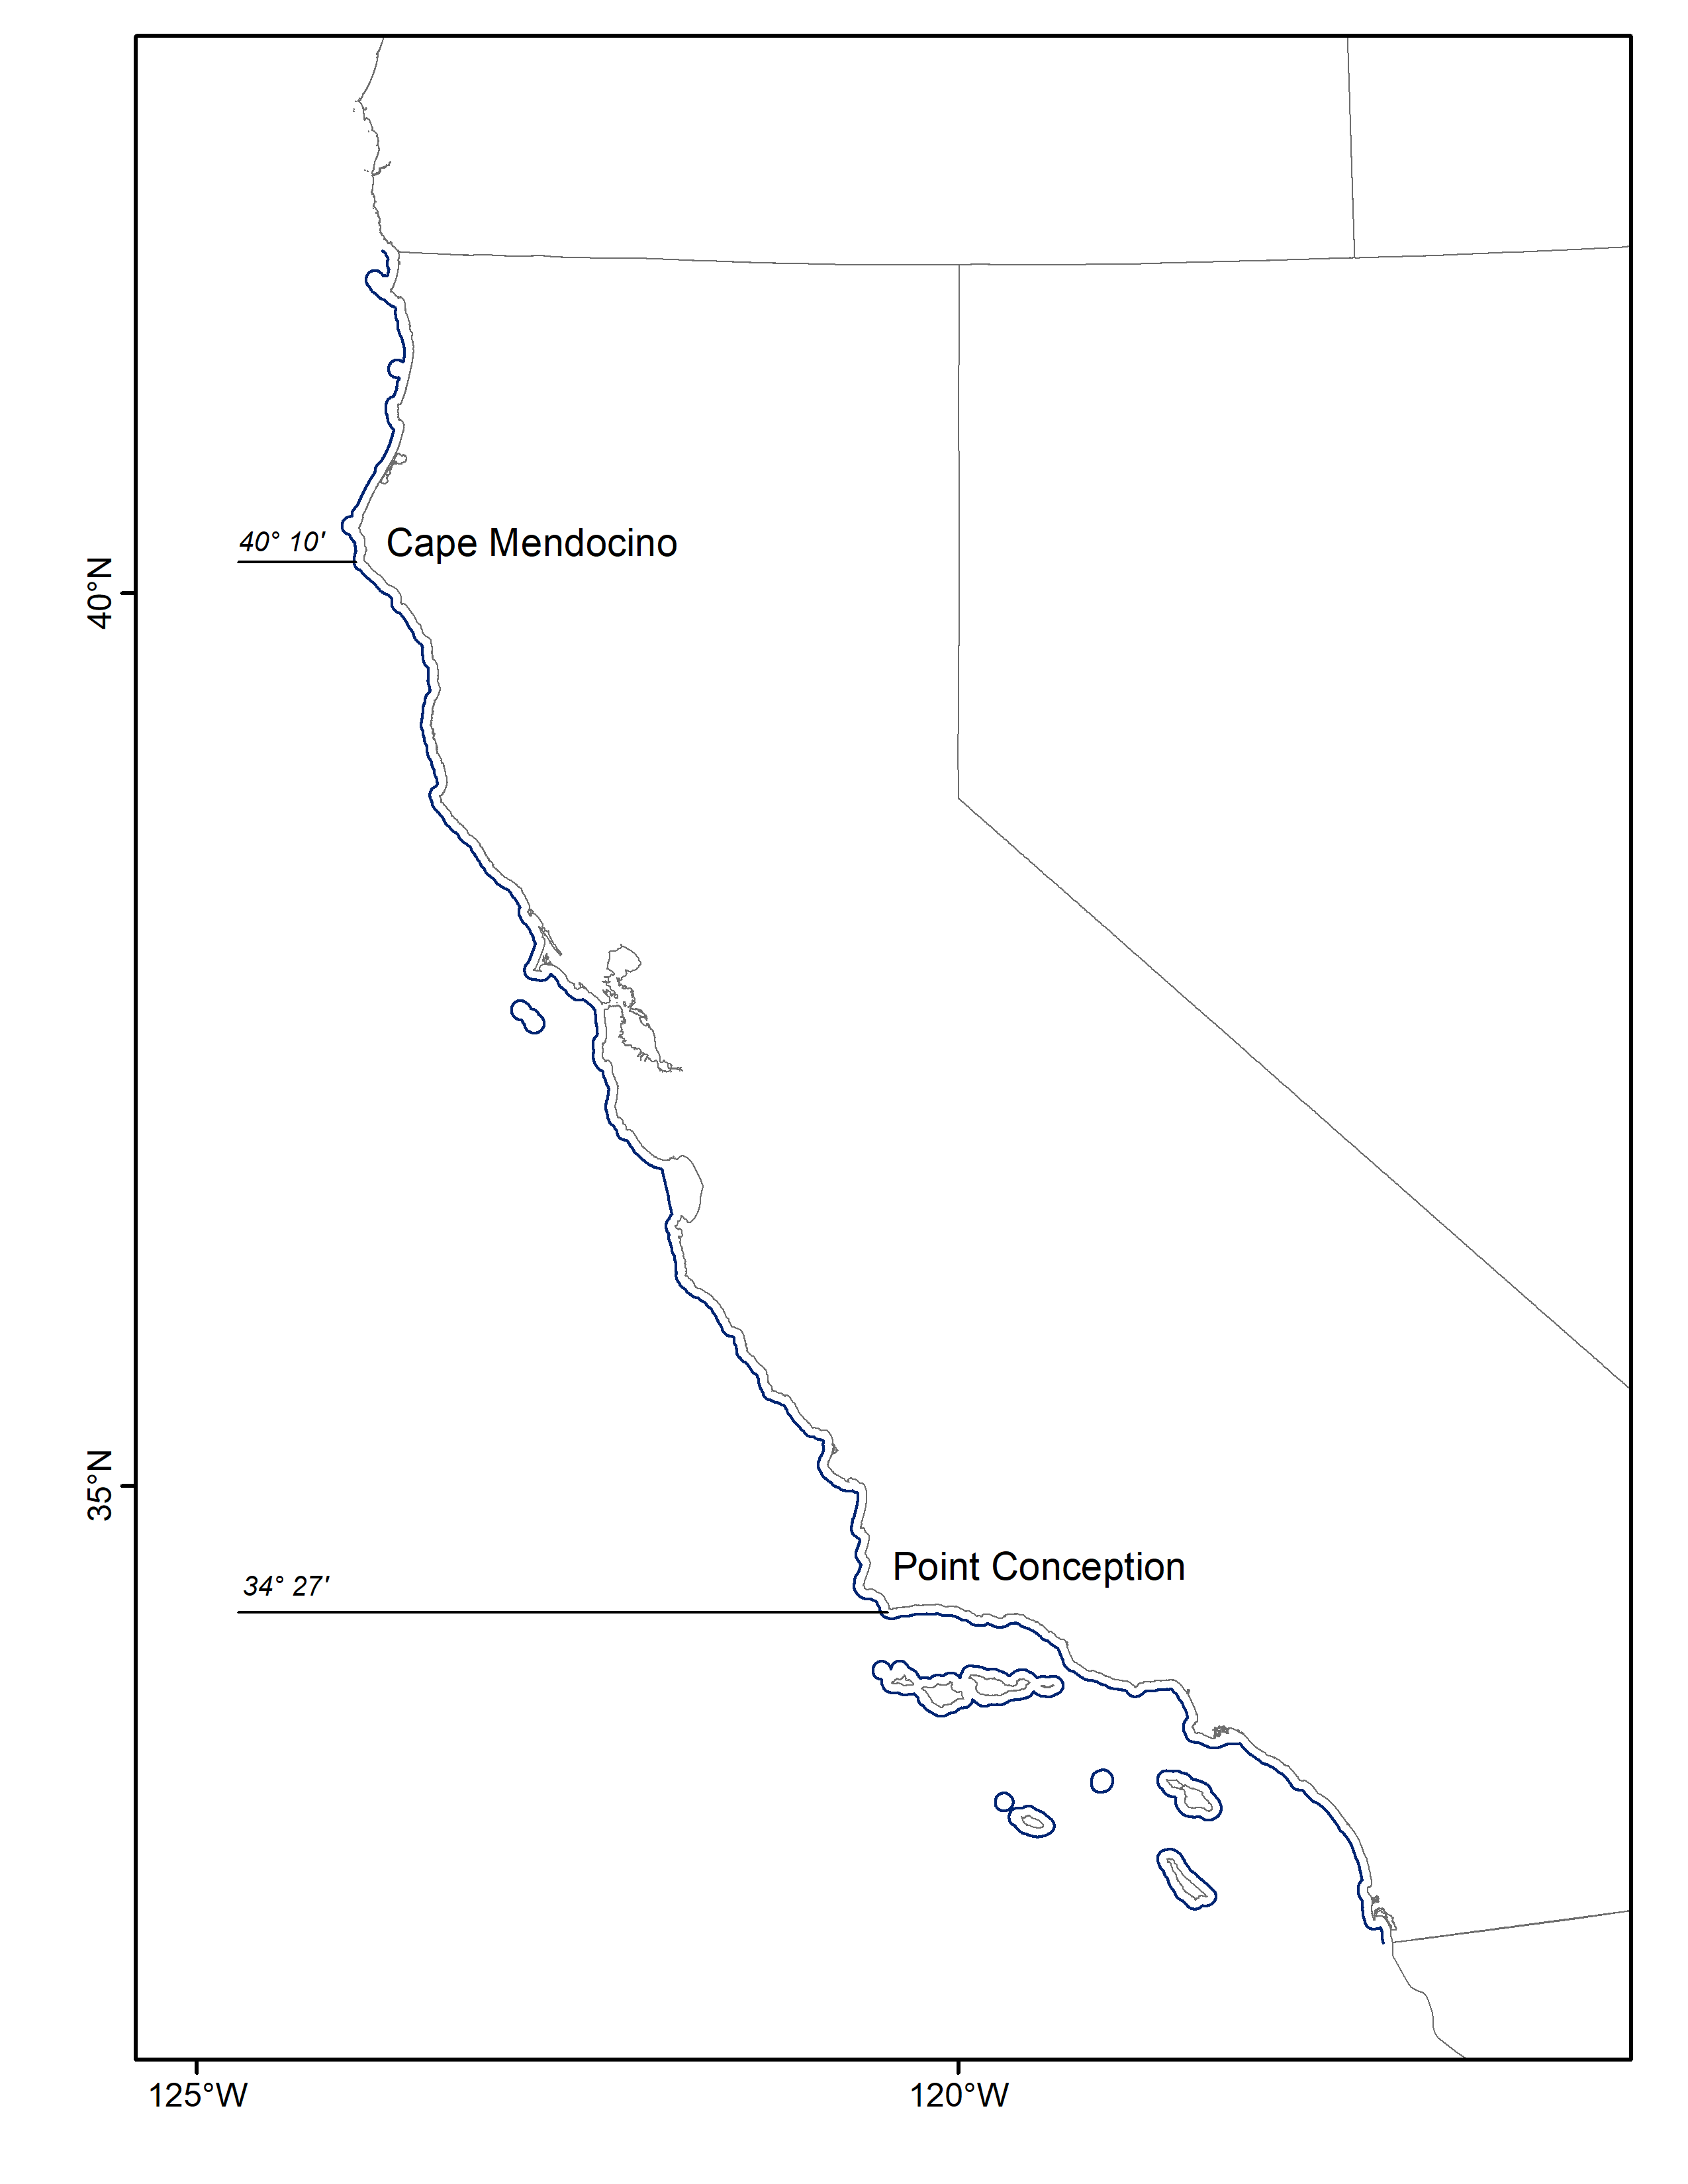
\includegraphics[width=1\textwidth,height=1\textheight]{C:/Stock_Assessments/VRML_Assessment_2021/GitHub/Vermilion_2021/doc/figures/assess_area.png}
\caption{Map of the assssment area with the 3 nm California stat water boundary. The northern California model includes areas from Point Conception to the California-Oregon border and the southern California assessment includes areas from Point Concpetion to the USA-Mexico border.\label{fig:assess-area}}
\end{figure}

\begin{figure}
\centering
\includegraphics[width=1\textwidth,height=1\textheight]{C:/Stock_Assessments/VRML_Assessment_2021/Model_files/NCA/Verm21NoCA_077_proposed_base_using_SS_OPT/plots/catch2 landings stacked.png}
\caption{Catches by fleet used in the base model.\label{fig:catch}}
\end{figure}

\begin{figure}
\centering
\includegraphics[width=0.6\textwidth,height=0.6\textheight]{C:/Stock_Assessments/VRML_Assessment_2021/Model_files/NCA/Verm21NoCA_077_proposed_base_using_SS_OPT//plots/comp_lendat_bubflt11mkt0.png}
\caption{Length composition data from the commercial hook-and-line fishery.\label{fig:len-data-COM-HKL}}
\end{figure}

\begin{figure}
\centering
\includegraphics[width=0.6\textwidth,height=0.6\textheight]{C:/Stock_Assessments/VRML_Assessment_2021/Model_files/NCA/Verm21NoCA_077_proposed_base_using_SS_OPT//plots/comp_lendat_bubflt2mkt0.png}
\caption{Length composition data from the commercial trawl fishery.\label{fig:len-data-COM-TWL}}
\end{figure}

\begin{figure}
\centering
\includegraphics[width=0.6\textwidth,height=0.6\textheight]{C:/Stock_Assessments/VRML_Assessment_2021/Model_files/NCA/Verm21NoCA_077_proposed_base_using_SS_OPT//plots/comp_lendat_bubflt3mkt0.png}
\caption{Length composition data from the commercial net fishery.\label{fig:len-data-COM-NET}}
\end{figure}

\begin{figure}
\centering
\includegraphics[width=0.6\textwidth,height=0.6\textheight]{C:/Stock_Assessments/VRML_Assessment_2021/Model_files/NCA/Verm21NoCA_077_proposed_base_using_SS_OPT//plots/comp_lendat_bubflt4mkt0_page2.png}
\caption{Length composition data from the recreational PC retained fishery.\label{fig:len-data-REC-PC}}
\end{figure}

\begin{figure}
\centering
\includegraphics[width=0.6\textwidth,height=0.6\textheight]{C:/Stock_Assessments/VRML_Assessment_2021/Model_files/NCA/Verm21NoCA_077_proposed_base_using_SS_OPT//plots/comp_lendat_bubflt5mkt0.png}
\caption{Length composition data from the recreational PC discard fishery.\label{fig:len-data-REC-PC-DIS}}
\end{figure}

\begin{figure}
\centering
\includegraphics[width=0.6\textwidth,height=0.6\textheight]{C:/Stock_Assessments/VRML_Assessment_2021/Model_files/NCA/Verm21NoCA_077_proposed_base_using_SS_OPT//plots/comp_lendat_bubflt6mkt0_page2.png}
\caption{Length composition data from the recreational PR retained fishery.\label{fig:len-data-REC-PR}}
\end{figure}

\begin{figure}
\centering
\includegraphics[width=0.6\textwidth,height=0.6\textheight]{C:/Stock_Assessments/VRML_Assessment_2021/Model_files/NCA/Verm21NoCA_077_proposed_base_using_SS_OPT//plots/comp_lendat_bubflt8mkt0.png}
\caption{Length composition data from the Deb Wilson-Vandenberg onboard survey.\label{fig:len-data-DWV-ONBOARD}}
\end{figure}

\begin{figure}
\centering
\includegraphics[width=0.6\textwidth,height=0.6\textheight]{C:/Stock_Assessments/VRML_Assessment_2021/Model_files/NCA/Verm21NoCA_077_proposed_base_using_SS_OPT//plots/comp_lendat_bubflt9mkt0.png}
\caption{Length composition data from the West coast groundfish bottomfish trawl survey.\label{fig:len-data-NWFSC-TWL}}
\end{figure}

\begin{figure}
\centering
\includegraphics[width=0.6\textwidth,height=0.6\textheight]{C:/Stock_Assessments/VRML_Assessment_2021/Model_files/NCA/Verm21NoCA_077_proposed_base_using_SS_OPT//plots/comp_lendat_bubflt11mkt0.png}
\caption{Length composition data from the Abrams thesis research survey.\label{fig:len-data-ABRAMS-RESEARCH}}
\end{figure}

\begin{figure}
\centering
\includegraphics[width=0.6\textwidth,height=0.6\textheight]{C:/Stock_Assessments/VRML_Assessment_2021/Model_files/NCA/Verm21NoCA_077_proposed_base_using_SS_OPT//plots/comp_lendat_bubflt12mkt0.png}
\caption{Length composition data from the SWFSC groundfish ecology survey.\label{fig:len-data-SWFSC-GF-ECOL}}
\end{figure}

\begin{figure}
\centering
\includegraphics[width=0.6\textwidth,height=0.6\textheight]{C:/Stock_Assessments/VRML_Assessment_2021/Model_files/NCA/Verm21NoCA_077_proposed_base_using_SS_OPT//plots/comp_lendat_bubflt13mkt0.png}
\caption{Length composition data from the California Collaborative Fisheries Research Project survey.\label{fig:len-data-CCFRP}}
\end{figure}

\begin{figure}
\centering
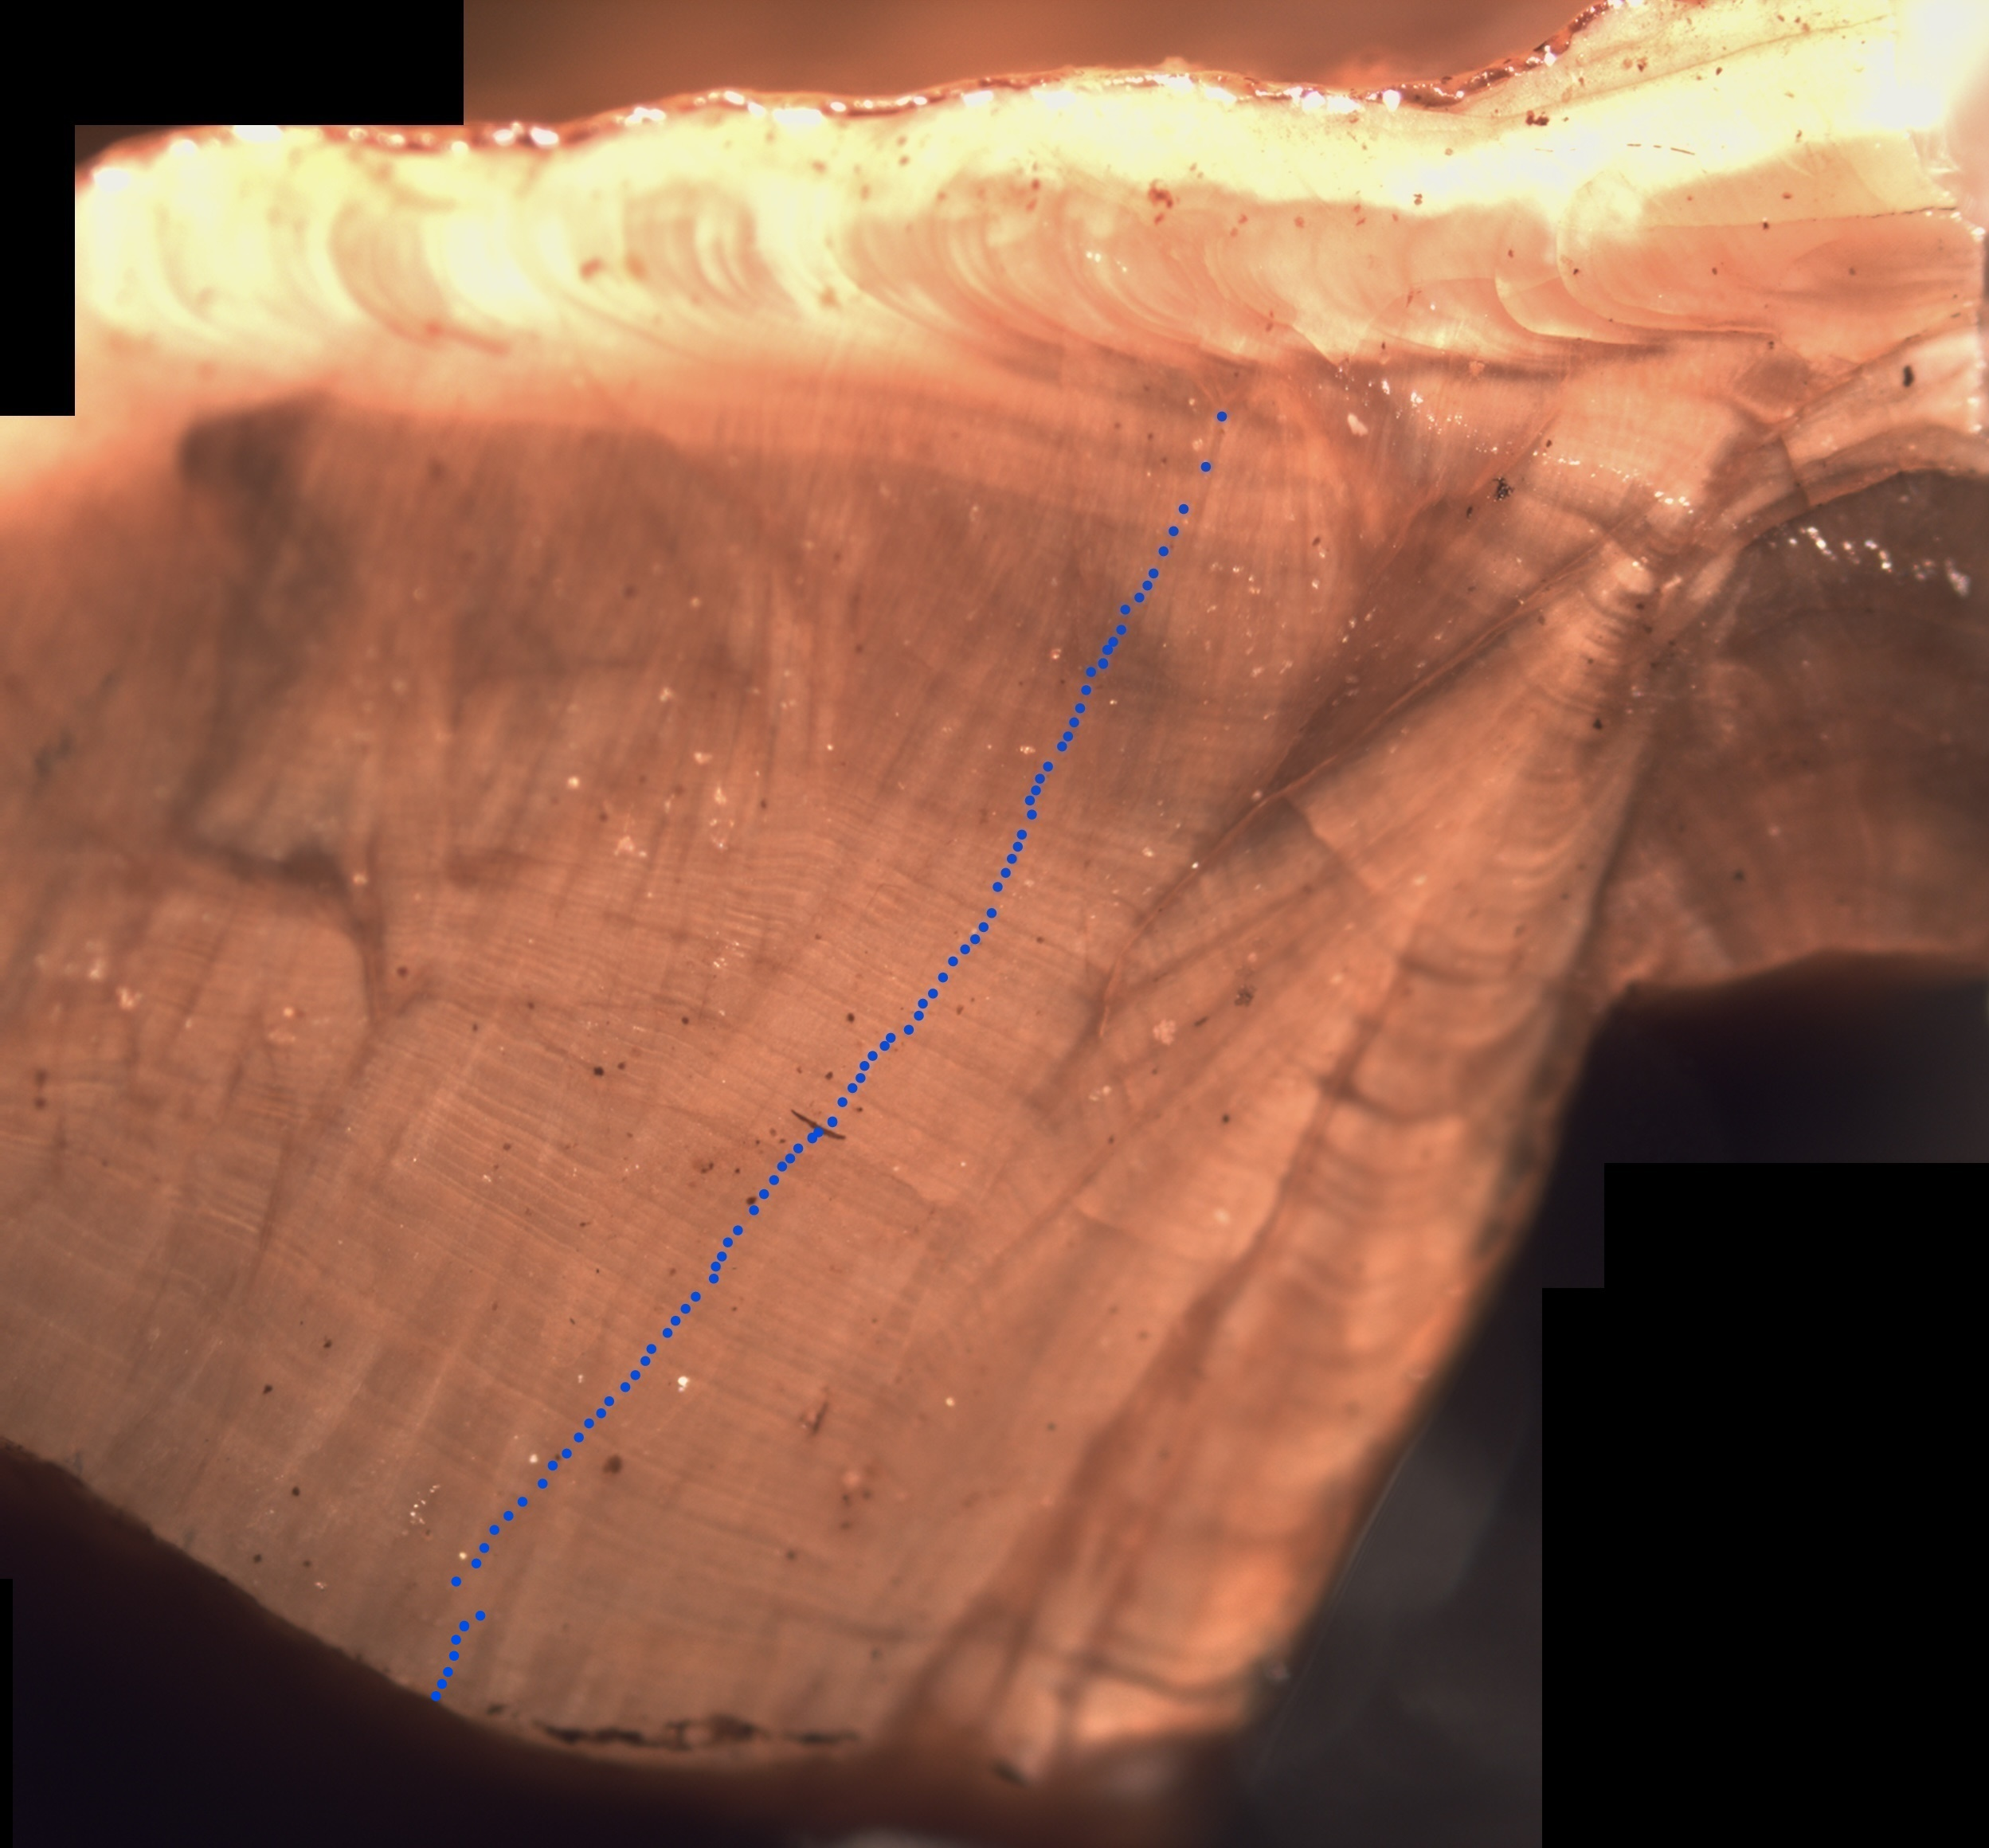
\includegraphics[width=1\textwidth,height=1\textheight]{C:/Stock_Assessments/VRML_Assessment_2021/GitHub/Vermilion_2021/doc/figures/oldfish.jpg}
\caption{Photograph of the \emph{oldest} aged fish used in the assessment with annuli marked by B. Kamikawa (NWFSC).\label{fig:oldfish}}
\end{figure}

\begin{figure}
\centering
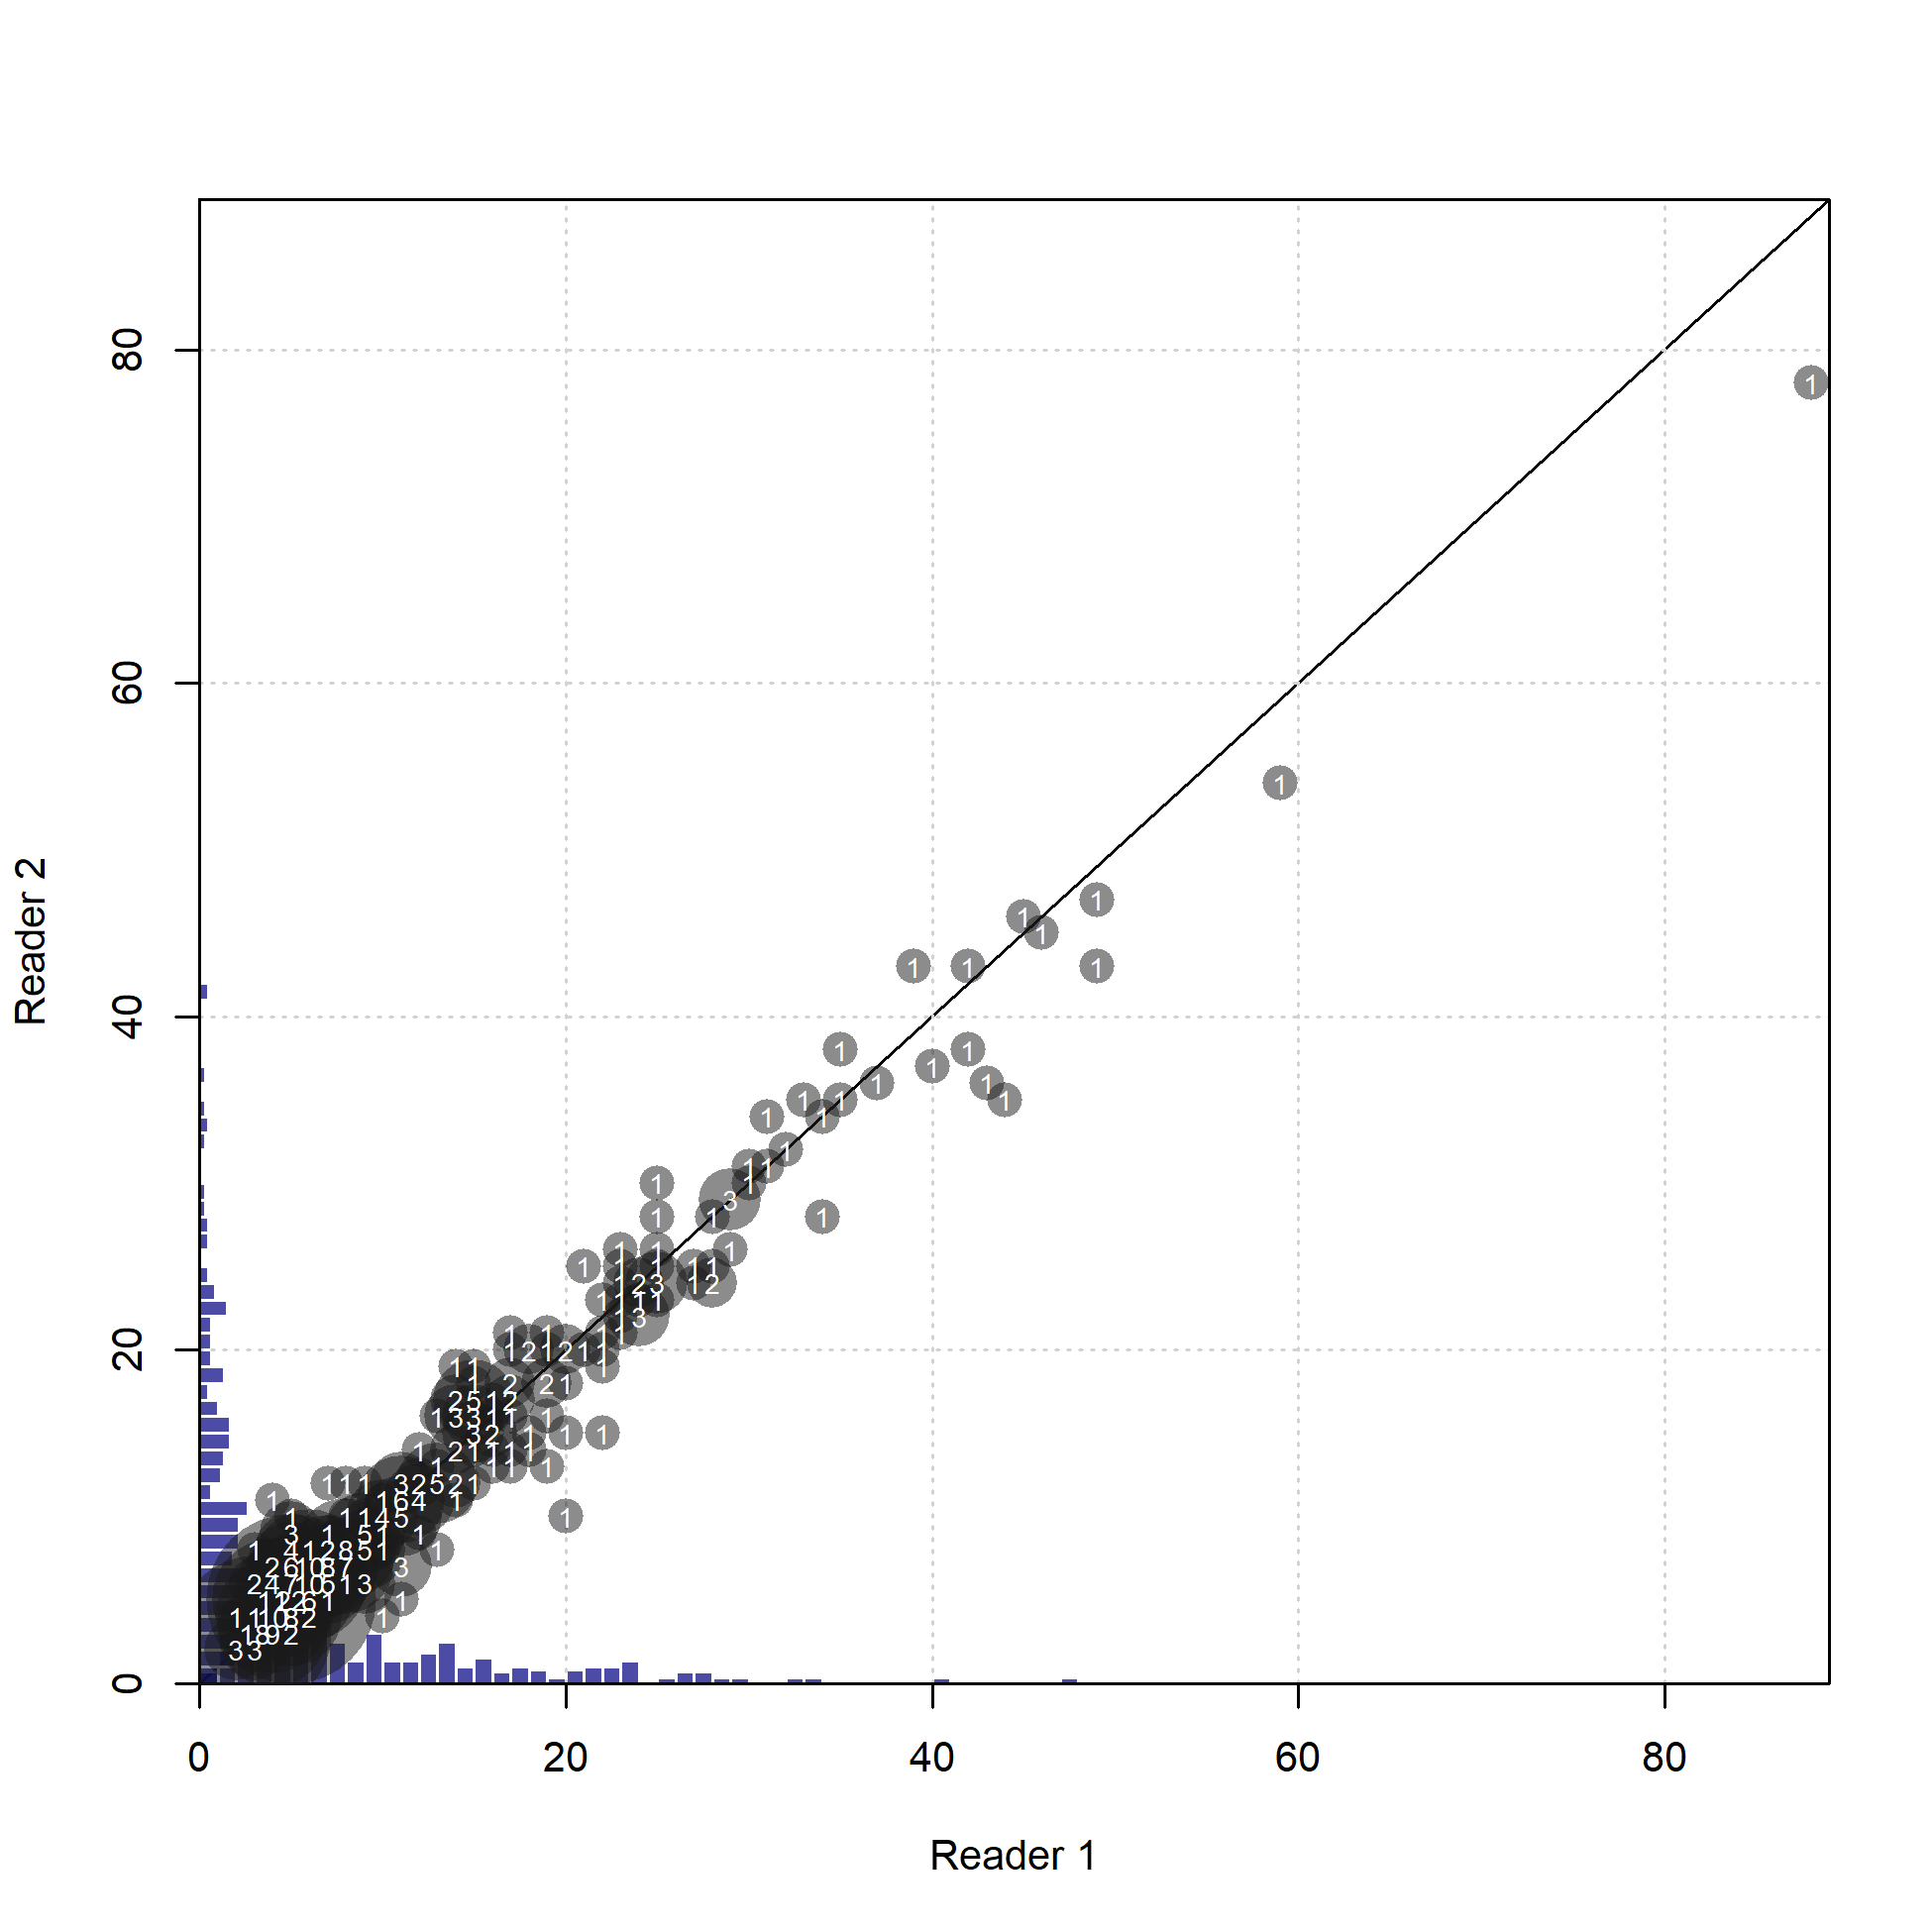
\includegraphics[width=1\textwidth,height=1\textheight]{C:/Stock_Assessments/VRML_Assessment_2021/GitHub/Vermilion_2021/doc/figures/Reader 1 vs Reader 2.png}
\caption{Aging precision between initial and blind double reads for vermilion. Numbers in the bubbles are the sample sizes of otoliths cross-read.\label{fig:reader1reader2}}
\end{figure}

\begin{figure}
\centering
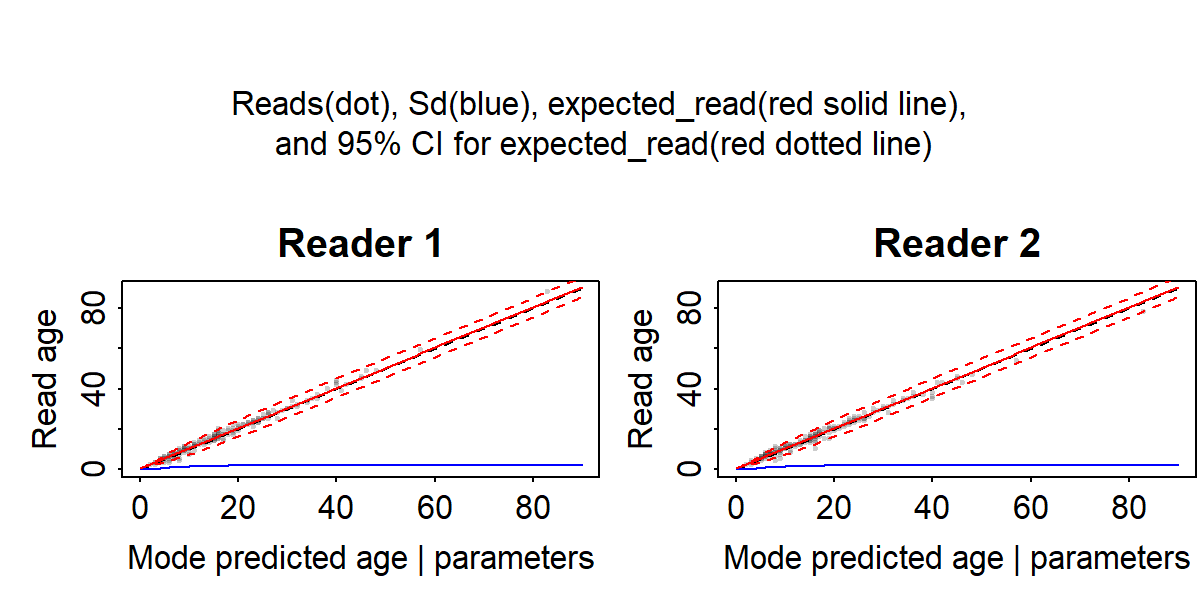
\includegraphics[width=1\textwidth,height=1\textheight]{C:/Stock_Assessments/VRML_Assessment_2021/GitHub/Vermilion_2021/doc/figures/True vs Reads (by reader).png}
\caption{True versus predicted age for two current age readers at the NWFSC from the ageing error software with unbiased reads for reader 1 and curvilinear bias for reader 1 and curvilinear standard deviation for both readers.\label{fig:truereads}}
\end{figure}

\begin{figure}
\centering
\includegraphics[width=1\textwidth,height=1\textheight]{C:/Stock_Assessments/VRML_Assessment_2021/Model_files/NCA/Verm21NoCA_077_proposed_base_using_SS_OPT//plots/numbers10_ageerror_matrix_1.png}
\caption{Distribution of observed age at true age for ageing error type 1.\label{fig:ageerror}}
\end{figure}

\begin{figure}
\centering
\includegraphics[width=1\textwidth,height=1\textheight]{C:/Stock_Assessments/VRML_Assessment_2021/Model_files/NCA/Verm21NoCA_077_proposed_base_using_SS_OPT//plots/bio5_weightatsize.png}
\caption{Weight-length relationship.\label{fig:weightlength}}
\end{figure}

\begin{figure}
\centering
\includegraphics[width=1\textwidth,height=1\textheight]{C:/Stock_Assessments/VRML_Assessment_2021/Model_files/NCA/Verm21NoCA_077_proposed_base_using_SS_OPT//plots/bio6_maturity.png}
\caption{Maturity at length.\label{fig:maturity}}
\end{figure}

\begin{figure}
\centering
\includegraphics[width=1\textwidth,height=1\textheight]{C:/Stock_Assessments/VRML_Assessment_2021/Model_files/NCA/Verm21NoCA_077_proposed_base_using_SS_OPT//plots/bio8_fecundity_wt.png}
\caption{Fecundity as a function of weight.\label{fig:fecundity}}
\end{figure}

\begin{figure}
\centering
\includegraphics[width=1\textwidth,height=1\textheight]{C:/Stock_Assessments/VRML_Assessment_2021/Model_files/NCA/Verm21NoCA_077_proposed_base_using_SS_OPT//plots/bio11_spawningoutput_age.png}
\caption{Spawning output at age. This is the product of maturity and fecundity. When these processes are length-based they are converted into the age dimension using the matrix of length at age.\label{fig:spawningoutputage}}
\end{figure}

\FloatBarrier

\begin{figure}
\centering
\includegraphics[width=1\textwidth,height=1\textheight]{C:/Stock_Assessments/VRML_Assessment_2021/Model_files/NCA/Verm21NoCA_077_proposed_base_using_SS_OPT//plots/bio1_sizeatage.png}
\caption{Length at age in the beginning of the year (or season) in the ending year of the model. Shaded area indicates 95\% distribution of length at age around estimated growth curve.\label{fig:fittedgrowth}}
\end{figure}

\FloatBarrier

\begin{figure}
\centering
\includegraphics[width=1\textwidth,height=1\textheight]{C:/Stock_Assessments/VRML_Assessment_2021/Model_files/NCA/Verm21NoCA_077_proposed_base_using_SS_OPT//plots/sel01_multiple_fleets_length1.png}
\caption{Selectivity at length by fleet.\label{fig:selex-length-all}}
\end{figure}

\FloatBarrier

\begin{figure}
\centering
\includegraphics[width=1\textwidth,height=1\textheight]{C:/Stock_Assessments/VRML_Assessment_2021/Model_files/NCA/Verm21NoCA_077_proposed_base_using_SS_OPT//plots/sel02_multiple_fleets_age1.png}
\caption{Selectivity at age derived from selectivity at length for multiple fleets.\label{fig:selex-age-all}}
\end{figure}

\begin{figure}
\centering
\includegraphics[width=1\textwidth,height=1\textheight]{C:/Stock_Assessments/VRML_Assessment_2021/Model_files/NCA/Verm21NoCA_077_proposed_base_using_SS_OPT//plots/sel03_len_timevary_surf_flt4sex1.png}
\caption{Surface plot of Female time-varying selectivity for REC\_PC.\label{fig:sel03_len_timevary_surf_flt4sex1}}
\end{figure}

\begin{figure}
\centering
\includegraphics[width=1\textwidth,height=1\textheight]{C:/Stock_Assessments/VRML_Assessment_2021/Model_files/NCA/Verm21NoCA_077_proposed_base_using_SS_OPT//plots/sel03_len_timevary_surf_flt6sex1.png}
\caption{Surface plot of Female time-varying selectivity for REC\_PR.\label{fig:sel03_len_timevary_surf_flt6sex1}}
\end{figure}

\FloatBarrier

\FloatBarrier

\begin{figure}
\centering
\includegraphics[width=1\textwidth,height=1\textheight]{C:/Stock_Assessments/VRML_Assessment_2021/Model_files/NCA/Verm21NoCA_077_proposed_base_using_SS_OPT//plots/sel09_len_flt1sex1.png}
\caption{Female ending year selectivity for the commercial hook-and-line fishery.\label{fig:endyr-selex-COM-HKL}}
\end{figure}

\begin{figure}
\centering
\includegraphics[width=1\textwidth,height=1\textheight]{C:/Stock_Assessments/VRML_Assessment_2021/Model_files/NCA/Verm21NoCA_077_proposed_base_using_SS_OPT//plots/sel09_len_flt2sex1.png}
\caption{Female ending year selectivity for the commercial trawl fishery.\label{fig:endyr-selex-COM-TWL}}
\end{figure}

\begin{figure}
\centering
\includegraphics[width=1\textwidth,height=1\textheight]{C:/Stock_Assessments/VRML_Assessment_2021/Model_files/NCA/Verm21NoCA_077_proposed_base_using_SS_OPT//plots/sel09_len_flt3sex1.png}
\caption{Female ending year selectivity for the commercial net fishery.\label{fig:endyr-selex-COM-NET}}
\end{figure}

\begin{figure}
\centering
\includegraphics[width=1\textwidth,height=1\textheight]{C:/Stock_Assessments/VRML_Assessment_2021/Model_files/NCA/Verm21NoCA_077_proposed_base_using_SS_OPT//plots/sel09_len_flt4sex1.png}
\caption{Female ending year selectivity for the recreational PC retained fishery.\label{fig:endyr-selex-REC-PC}}
\end{figure}

\begin{figure}
\centering
\includegraphics[width=1\textwidth,height=1\textheight]{C:/Stock_Assessments/VRML_Assessment_2021/Model_files/NCA/Verm21NoCA_077_proposed_base_using_SS_OPT//plots/sel09_len_flt5sex1.png}
\caption{Female ending year selectivity for the recreational PC discard fishery.\label{fig:endyr-selex-REC-PC-DIS}}
\end{figure}

\begin{figure}
\centering
\includegraphics[width=1\textwidth,height=1\textheight]{C:/Stock_Assessments/VRML_Assessment_2021/Model_files/NCA/Verm21NoCA_077_proposed_base_using_SS_OPT//plots/sel09_len_flt6sex1.png}
\caption{Female ending year selectivity for the recreational PR retained fishery.\label{fig:endyr-selex-REC-PR}}
\end{figure}

\begin{figure}
\centering
\includegraphics[width=1\textwidth,height=1\textheight]{C:/Stock_Assessments/VRML_Assessment_2021/Model_files/NCA/Verm21NoCA_077_proposed_base_using_SS_OPT//plots/sel09_len_flt9sex1.png}
\caption{Female ending year selectivity for the West coast groundfish bottomfish trawl survey.\label{fig:endyr-selex-NWFSC-TWL}}
\end{figure}

\begin{figure}
\centering
\includegraphics[width=1\textwidth,height=1\textheight]{C:/Stock_Assessments/VRML_Assessment_2021/Model_files/NCA/Verm21NoCA_077_proposed_base_using_SS_OPT//plots/sel09_len_flt7sex1.png}
\caption{Female ending year selectivity for the recreational PR discard fishery.\label{fig:endyr-selex-REC-PR-DIS}}
\end{figure}

\FloatBarrier

\begin{figure}
\centering
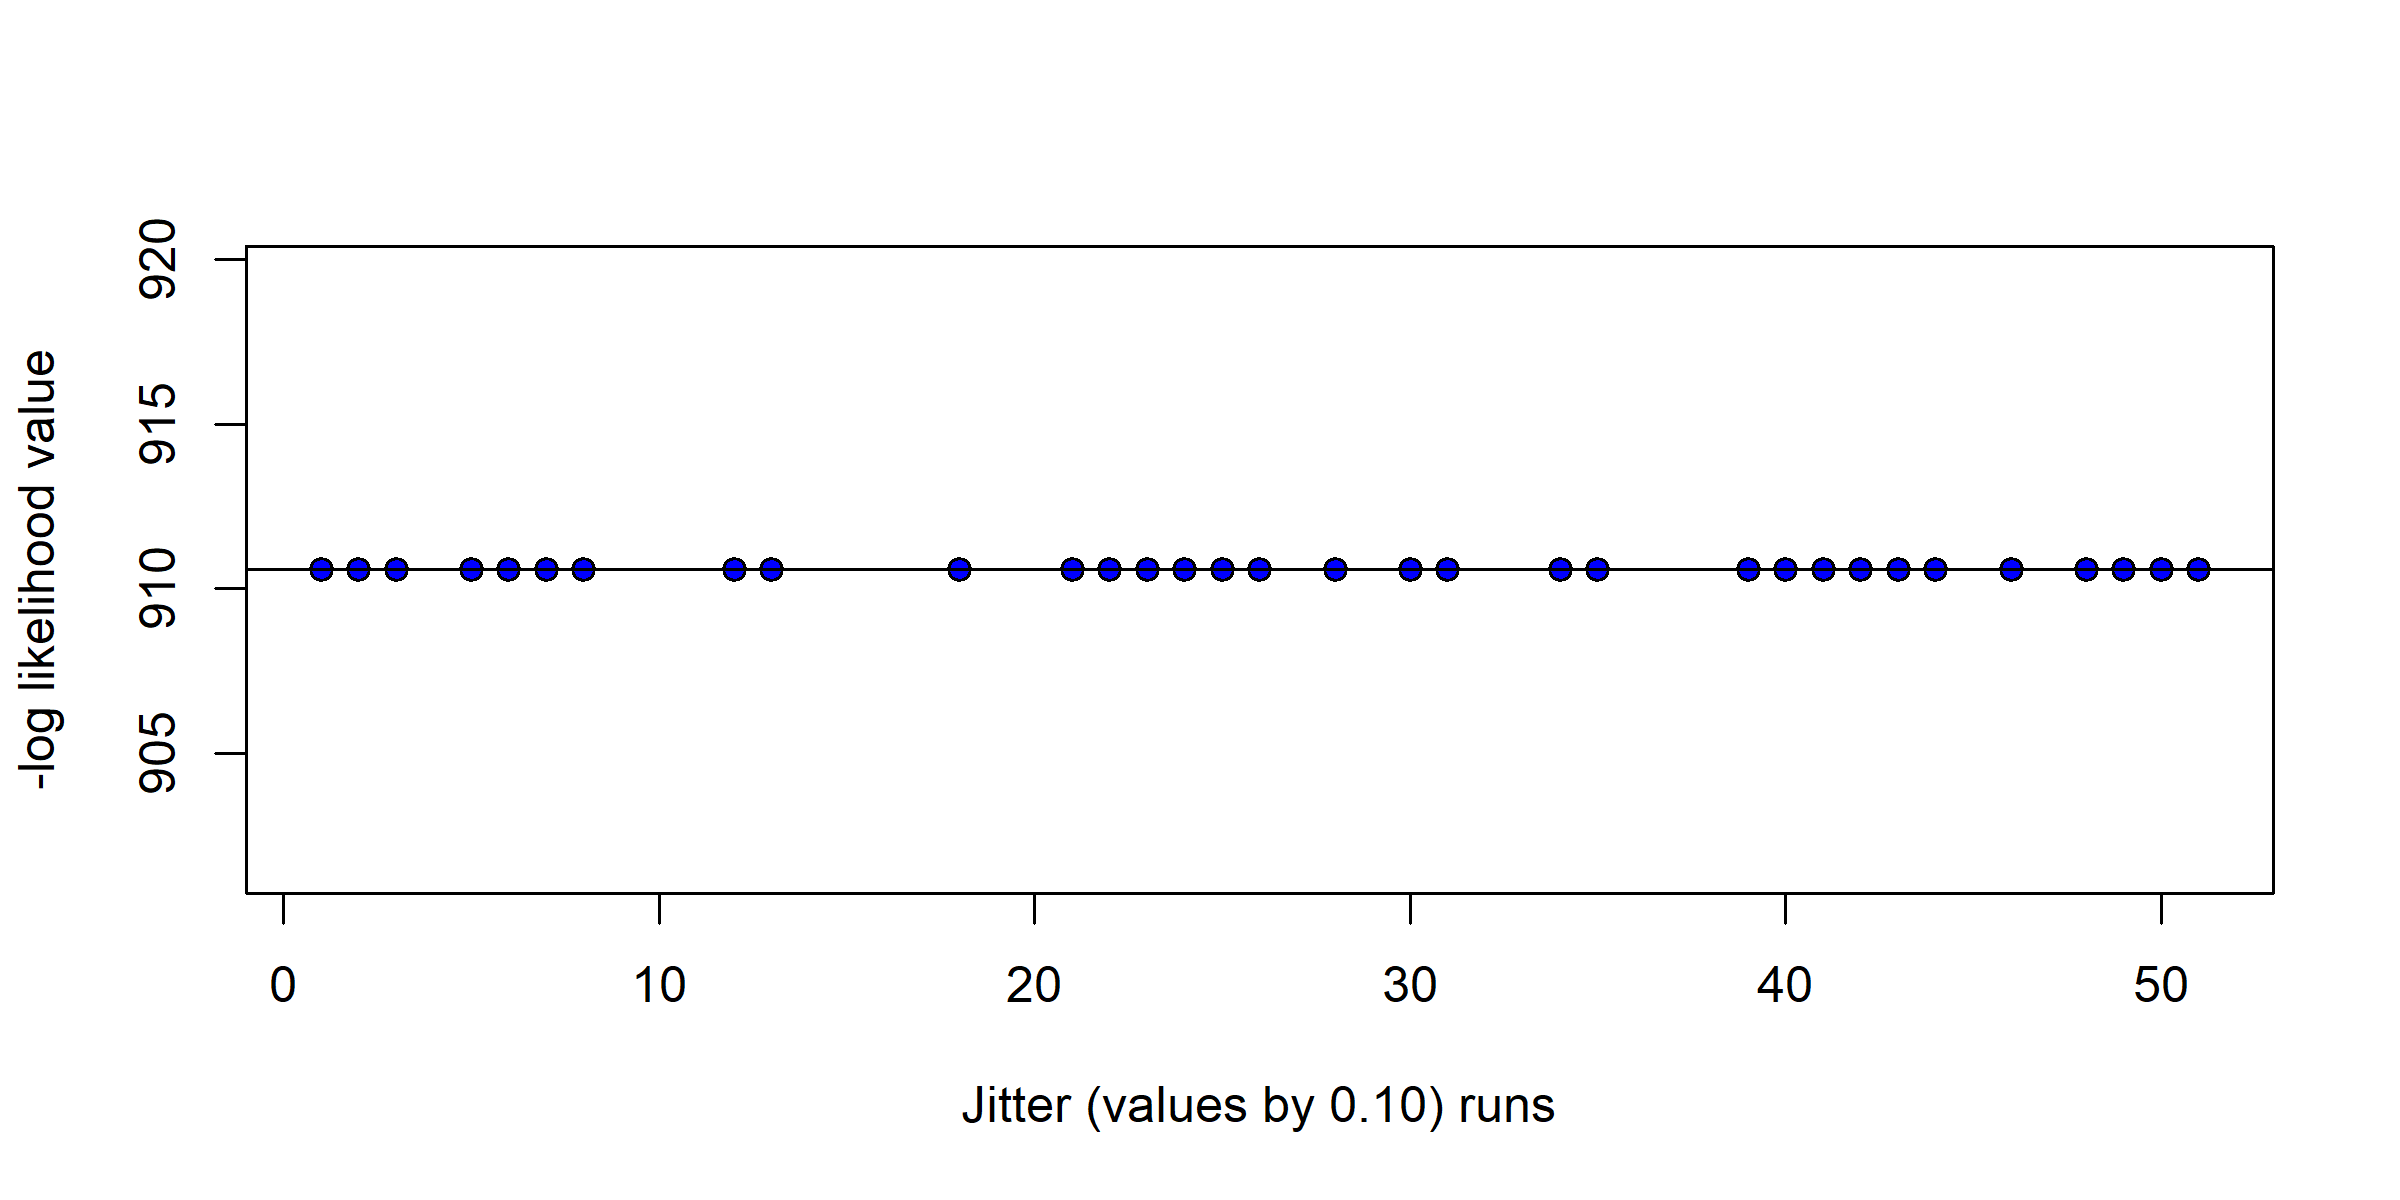
\includegraphics[width=1\textwidth,height=1\textheight]{C:/Stock_Assessments/VRML_Assessment_2021/GitHub/Vermilion_2021/doc/figures/jitter_NCA.png}
\caption{Results from 50 jittered runs of the pre-STAR base model. Missing values indicate the run did not converge.\label{fig:jitter}}
\end{figure}

\FloatBarrier

\FloatBarrier

\begin{figure}
\centering
\includegraphics[width=1\textwidth,height=1\textheight]{C:/Stock_Assessments/VRML_Assessment_2021/Model_files/NCA/Verm21NoCA_077_proposed_base_using_SS_OPT//plots/comp_lenfit__aggregated_across_time.png}
\caption{Length comps, aggregated across time by fleet. Labels `retained' and `discard' indicate discarded or retained sampled for each fleet. Panels without this designation represent the whole catch.\label{fig:lenfits-all}}
\end{figure}

\FloatBarrier

\begin{figure}
\centering
\includegraphics[width=1\textwidth,height=1\textheight]{C:/Stock_Assessments/VRML_Assessment_2021/Model_files/NCA/Verm21NoCA_077_proposed_base_using_SS_OPT//plots/comp_lenfit_residsflt11mkt0.png}
\caption{Pearson residuals for the commercial hook-and-line fishery. Closed bubbles are positive residuals (observed \textgreater{} expected) and open bubbles are negative residuals (observed \textless{} expected).\label{fig:len-pearson-COM-HKL}}
\end{figure}

\begin{figure}
\centering
\includegraphics[width=1\textwidth,height=1\textheight]{C:/Stock_Assessments/VRML_Assessment_2021/Model_files/NCA/Verm21NoCA_077_proposed_base_using_SS_OPT//plots/comp_lenfit_data_weighting_TA1.8_COM_HKL.png}
\caption{Mean length for REC\_PR with 95\% confidence intervals based on current samples sizes. Francis data weighting method TA1.8: thinner intervals (with capped ends) show result of further adjusting sample sizes based on suggested multiplier (with 95\% interval) for length data from the commercial hook-and-line fishery.\label{fig:mean-len-fit-COM-HKL}}
\end{figure}

\begin{figure}
\centering
\includegraphics[width=1\textwidth,height=1\textheight]{C:/Stock_Assessments/VRML_Assessment_2021/Model_files/NCA/Verm21NoCA_077_proposed_base_using_SS_OPT//plots/comp_lenfit_residsflt2mkt0.png}
\caption{Pearson residuals for the commercial trawl fishery. Closed bubbles are positive residuals (observed \textgreater{} expected) and open bubbles are negative residuals (observed \textless{} expected).\label{fig:len-pearson-COM-TWL}}
\end{figure}

\begin{figure}
\centering
\includegraphics[width=1\textwidth,height=1\textheight]{C:/Stock_Assessments/VRML_Assessment_2021/Model_files/NCA/Verm21NoCA_077_proposed_base_using_SS_OPT//plots/comp_lenfit_data_weighting_TA1.8_COM_TWL.png}
\caption{Mean length for REC\_PR with 95\% confidence intervals based on current samples sizes. Francis data weighting method TA1.8: thinner intervals (with capped ends) show result of further adjusting sample sizes based on suggested multiplier (with 95\% interval) for length data from the commercial trawl fishery.\label{fig:mean-len-fit-COM-TWL}}
\end{figure}

\begin{figure}
\centering
\includegraphics[width=1\textwidth,height=1\textheight]{C:/Stock_Assessments/VRML_Assessment_2021/Model_files/NCA/Verm21NoCA_077_proposed_base_using_SS_OPT//plots/comp_lenfit_residsflt3mkt0.png}
\caption{Pearson residuals for the commercial net fishery. Closed bubbles are positive residuals (observed \textgreater{} expected) and open bubbles are negative residuals (observed \textless{} expected).\label{fig:len-pearson-COM-NET}}
\end{figure}

\begin{figure}
\centering
\includegraphics[width=1\textwidth,height=1\textheight]{C:/Stock_Assessments/VRML_Assessment_2021/Model_files/NCA/Verm21NoCA_077_proposed_base_using_SS_OPT//plots/comp_lenfit_data_weighting_TA1.8_COM_NET.png}
\caption{Mean length for REC\_PR with 95\% confidence intervals based on current samples sizes. Francis data weighting method TA1.8: thinner intervals (with capped ends) show result of further adjusting sample sizes based on suggested multiplier (with 95\% interval) for length data from the commercial net fishery.\label{fig:mean-len-fit-COM-NET}}
\end{figure}

\begin{figure}
\centering
\includegraphics[width=1\textwidth,height=1\textheight]{C:/Stock_Assessments/VRML_Assessment_2021/Model_files/NCA/Verm21NoCA_077_proposed_base_using_SS_OPT//plots/comp_lenfit_residsflt4mkt0_page2.png}
\caption{Pearson residuals for the recreational PC retained fishery. Closed bubbles are positive residuals (observed \textgreater{} expected) and open bubbles are negative residuals (observed \textless{} expected).\label{fig:len-pearson-REC-PC}}
\end{figure}

\begin{figure}
\centering
\includegraphics[width=1\textwidth,height=1\textheight]{C:/Stock_Assessments/VRML_Assessment_2021/Model_files/NCA/Verm21NoCA_077_proposed_base_using_SS_OPT//plots/comp_lenfit_data_weighting_TA1.8_REC_PC.png}
\caption{Mean length for REC\_PR with 95\% confidence intervals based on current samples sizes. Francis data weighting method TA1.8: thinner intervals (with capped ends) show result of further adjusting sample sizes based on suggested multiplier (with 95\% interval) for length data from the recreational PC retained fishery.\label{fig:mean-len-fit-REC-PC}}
\end{figure}

\begin{figure}
\centering
\includegraphics[width=1\textwidth,height=1\textheight]{C:/Stock_Assessments/VRML_Assessment_2021/Model_files/NCA/Verm21NoCA_077_proposed_base_using_SS_OPT//plots/comp_lenfit_residsflt5mkt0.png}
\caption{Pearson residuals for the recreational PC discard fishery. Closed bubbles are positive residuals (observed \textgreater{} expected) and open bubbles are negative residuals (observed \textless{} expected).\label{fig:len-pearson-REC-PC-DIS}}
\end{figure}

\begin{figure}
\centering
\includegraphics[width=1\textwidth,height=1\textheight]{C:/Stock_Assessments/VRML_Assessment_2021/Model_files/NCA/Verm21NoCA_077_proposed_base_using_SS_OPT//plots/comp_lenfit_data_weighting_TA1.8_REC_PC_DIS.png}
\caption{Mean length for REC\_PR with 95\% confidence intervals based on current samples sizes. Francis data weighting method TA1.8: thinner intervals (with capped ends) show result of further adjusting sample sizes based on suggested multiplier (with 95\% interval) for length data from the recreational PC discard fishery.\label{fig:mean-len-fit-REC-PC-DIS}}
\end{figure}

\begin{figure}
\centering
\includegraphics[width=1\textwidth,height=1\textheight]{C:/Stock_Assessments/VRML_Assessment_2021/Model_files/NCA/Verm21NoCA_077_proposed_base_using_SS_OPT//plots/comp_lenfit_residsflt6mkt0_page2.png}
\caption{Pearson residuals for the recreational PR retained fishery. Closed bubbles are positive residuals (observed \textgreater{} expected) and open bubbles are negative residuals (observed \textless{} expected).\label{fig:len-pearson-REC-PR}}
\end{figure}

\begin{figure}
\centering
\includegraphics[width=1\textwidth,height=1\textheight]{C:/Stock_Assessments/VRML_Assessment_2021/Model_files/NCA/Verm21NoCA_077_proposed_base_using_SS_OPT//plots/comp_lenfit_data_weighting_TA1.8_REC_PR.png}
\caption{Mean length for REC\_PR with 95\% confidence intervals based on current samples sizes. Francis data weighting method TA1.8: thinner intervals (with capped ends) show result of further adjusting sample sizes based on suggested multiplier (with 95\% interval) for length data from the recreational PR retained fishery.\label{fig:mean-len-fit-REC-PR}}
\end{figure}

\begin{figure}
\centering
\includegraphics[width=1\textwidth,height=1\textheight]{C:/Stock_Assessments/VRML_Assessment_2021/Model_files/NCA/Verm21NoCA_077_proposed_base_using_SS_OPT//plots/comp_lenfit_residsflt8mkt0.png}
\caption{Pearson residuals for the Deb Wilson-Vandenberg onboard survey. Closed bubbles are positive residuals (observed \textgreater{} expected) and open bubbles are negative residuals (observed \textless{} expected).\label{fig:len-pearson-DWV-ONBOARD}}
\end{figure}

\begin{figure}
\centering
\includegraphics[width=1\textwidth,height=1\textheight]{C:/Stock_Assessments/VRML_Assessment_2021/Model_files/NCA/Verm21NoCA_077_proposed_base_using_SS_OPT//plots/comp_lenfit_data_weighting_TA1.8_DWV_ONBOARD.png}
\caption{Mean length for REC\_PR with 95\% confidence intervals based on current samples sizes. Francis data weighting method TA1.8: thinner intervals (with capped ends) show result of further adjusting sample sizes based on suggested multiplier (with 95\% interval) for length data from the Deb Wilson-Vandenberg onboard survey.\label{fig:mean-len-fit-DWV-ONBOARD}}
\end{figure}

\begin{figure}
\centering
\includegraphics[width=1\textwidth,height=1\textheight]{C:/Stock_Assessments/VRML_Assessment_2021/Model_files/NCA/Verm21NoCA_077_proposed_base_using_SS_OPT//plots/comp_lenfit_residsflt9mkt0.png}
\caption{Pearson residuals for the West coast groundfish bottomfish trawl survey. Closed bubbles are positive residuals (observed \textgreater{} expected) and open bubbles are negative residuals (observed \textless{} expected).\label{fig:len-pearson-NWFSC-TWL}}
\end{figure}

\begin{figure}
\centering
\includegraphics[width=1\textwidth,height=1\textheight]{C:/Stock_Assessments/VRML_Assessment_2021/Model_files/NCA/Verm21NoCA_077_proposed_base_using_SS_OPT//plots/comp_lenfit_data_weighting_TA1.8_NWFSC_TWL.png}
\caption{Mean length for REC\_PR with 95\% confidence intervals based on current samples sizes. Francis data weighting method TA1.8: thinner intervals (with capped ends) show result of further adjusting sample sizes based on suggested multiplier (with 95\% interval) for length data from the West coast groundfish bottomfish trawl survey.\label{fig:mean-len-fit-NWFSC-TWL}}
\end{figure}

\begin{figure}
\centering
\includegraphics[width=1\textwidth,height=1\textheight]{C:/Stock_Assessments/VRML_Assessment_2021/Model_files/NCA/Verm21NoCA_077_proposed_base_using_SS_OPT//plots/comp_lenfit_residsflt11mkt0.png}
\caption{Pearson residuals for the Abrams thesis research survey. Closed bubbles are positive residuals (observed \textgreater{} expected) and open bubbles are negative residuals (observed \textless{} expected).\label{fig:len-pearson-ABRAMS-RESEARCH}}
\end{figure}

\begin{figure}
\centering
\includegraphics[width=1\textwidth,height=1\textheight]{C:/Stock_Assessments/VRML_Assessment_2021/Model_files/NCA/Verm21NoCA_077_proposed_base_using_SS_OPT//plots/comp_lenfit_data_weighting_TA1.8_ABRAMS_RESEARCH.png}
\caption{Mean length for REC\_PR with 95\% confidence intervals based on current samples sizes. Francis data weighting method TA1.8: thinner intervals (with capped ends) show result of further adjusting sample sizes based on suggested multiplier (with 95\% interval) for length data from the Abrams thesis research survey.\label{fig:mean-len-fit-ABRAMS-RESEARCH}}
\end{figure}

\begin{figure}
\centering
\includegraphics[width=1\textwidth,height=1\textheight]{C:/Stock_Assessments/VRML_Assessment_2021/Model_files/NCA/Verm21NoCA_077_proposed_base_using_SS_OPT//plots/comp_lenfit_residsflt12mkt0.png}
\caption{Pearson residuals for the SWFSC groundfish ecology survey. Closed bubbles are positive residuals (observed \textgreater{} expected) and open bubbles are negative residuals (observed \textless{} expected).\label{fig:len-pearson-SWFSC-GF-ECOL}}
\end{figure}

\begin{figure}
\centering
\includegraphics[width=1\textwidth,height=1\textheight]{C:/Stock_Assessments/VRML_Assessment_2021/Model_files/NCA/Verm21NoCA_077_proposed_base_using_SS_OPT//plots/comp_lenfit_data_weighting_TA1.8_SWFSC_GF_ECOL.png}
\caption{Mean length for REC\_PR with 95\% confidence intervals based on current samples sizes. Francis data weighting method TA1.8: thinner intervals (with capped ends) show result of further adjusting sample sizes based on suggested multiplier (with 95\% interval) for length data from the SWFSC groundfish ecology survey.\label{fig:mean-len-fit-SWFSC-GF-ECOL}}
\end{figure}

\begin{figure}
\centering
\includegraphics[width=1\textwidth,height=1\textheight]{C:/Stock_Assessments/VRML_Assessment_2021/Model_files/NCA/Verm21NoCA_077_proposed_base_using_SS_OPT//plots/comp_lenfit_residsflt13mkt0.png}
\caption{Pearson residuals for the California Collaborative Fisheries Research Project survey. Closed bubbles are positive residuals (observed \textgreater{} expected) and open bubbles are negative residuals (observed \textless{} expected).\label{fig:len-pearson-CCFRP}}
\end{figure}

\begin{figure}
\centering
\includegraphics[width=1\textwidth,height=1\textheight]{C:/Stock_Assessments/VRML_Assessment_2021/Model_files/NCA/Verm21NoCA_077_proposed_base_using_SS_OPT//plots/comp_lenfit_data_weighting_TA1.8_CCFRP.png}
\caption{Mean length for REC\_PR with 95\% confidence intervals based on current samples sizes. Francis data weighting method TA1.8: thinner intervals (with capped ends) show result of further adjusting sample sizes based on suggested multiplier (with 95\% interval) for length data from the California Collaborative Fisheries Research Project survey.\label{fig:mean-len-fit-CCFRP}}
\end{figure}

\FloatBarrier

\begin{figure}
\centering
\includegraphics[width=1\textwidth,height=1\textheight]{C:/Stock_Assessments/VRML_Assessment_2021/Model_files/NCA/Verm21NoCA_077_proposed_base_using_SS_OPT//plots/sexratio_len_flt11mkt0.png}
\caption{Sex ratios for length comps, whole catchAbrams thesis research survey. Observed sex ratios (points) with 75\% intervals (vertical lines) calculated as a Jeffreys interval based on the adjusted input sample size. The model expectation is shown in the purple line.\label{fig:sexratio-ABRAMS-RESEARCH}}
\end{figure}

\begin{figure}
\centering
\includegraphics[width=1\textwidth,height=1\textheight]{C:/Stock_Assessments/VRML_Assessment_2021/Model_files/NCA/Verm21NoCA_077_proposed_base_using_SS_OPT//plots/sexratio_len_flt12mkt0.png}
\caption{Sex ratios for length comps, whole catchSWFSC groundfish ecology survey. Observed sex ratios (points) with 75\% intervals (vertical lines) calculated as a Jeffreys interval based on the adjusted input sample size. The model expectation is shown in the purple line.\label{fig:sexratio-SWFSC-GF-ECOL}}
\end{figure}

\begin{figure}
\centering
\includegraphics[width=1\textwidth,height=1\textheight]{C:/Stock_Assessments/VRML_Assessment_2021/Model_files/NCA/Verm21NoCA_077_proposed_base_using_SS_OPT//plots/sexratio_len_flt9mkt0.png}
\caption{Sex ratios for length comps, whole catchWest coast groundfish bottomfish trawl survey. Observed sex ratios (points) with 75\% intervals (vertical lines) calculated as a Jeffreys interval based on the adjusted input sample size. The model expectation is shown in the purple line.\label{fig:sexratio-NWFSC-TWL}}
\end{figure}

\FloatBarrier

\begin{figure}
\centering
\includegraphics[width=1\textwidth,height=1\textheight]{C:/Stock_Assessments/VRML_Assessment_2021/Model_files/NCA/Verm21NoCA_077_proposed_base_using_SS_OPT//plots/index9_standcpueall.png}
\caption{Standardized indices overlaid. Each index is rescaled to have mean observation = 1.0.\label{fig:cpueall}}
\end{figure}

\begin{figure}
\centering
\includegraphics[width=1\textwidth,height=1\textheight]{C:/Stock_Assessments/VRML_Assessment_2021/Model_files/NCA/Verm21NoCA_077_proposed_base_using_SS_OPT//plots/index5_logcpuefit_REC_PC.png}
\caption{Fit to log index data on log scale for the recreational PC retained fishery. Lines indicate 95\% uncertainty interval around index values based on the model assumption of lognormal error. Thicker lines (if present) indicate input uncertainty before addition of estimated additional uncertainty parameter.\label{fig:log-cpue-REC-PC}}
\end{figure}

\begin{figure}
\centering
\includegraphics[width=1\textwidth,height=1\textheight]{C:/Stock_Assessments/VRML_Assessment_2021/Model_files/NCA/Verm21NoCA_077_proposed_base_using_SS_OPT//plots/index10_resids_SE_total_REC_PC.png}
\caption{Residuals of fit to index for the REC\_PC. Values are (log(Obs) - log(Exp))/SE where SE is the total standard error including any estimated additional uncertainty.\label{fig:cpue-resid-REC-PC}}
\end{figure}

\begin{figure}
\centering
\includegraphics[width=1\textwidth,height=1\textheight]{C:/Stock_Assessments/VRML_Assessment_2021/Model_files/NCA/Verm21NoCA_077_proposed_base_using_SS_OPT//plots/index5_logcpuefit_REC_PR.png}
\caption{Fit to log index data on log scale for the recreational PR retained fishery. Lines indicate 95\% uncertainty interval around index values based on the model assumption of lognormal error. Thicker lines (if present) indicate input uncertainty before addition of estimated additional uncertainty parameter.\label{fig:log-cpue-REC-PR}}
\end{figure}

\begin{figure}
\centering
\includegraphics[width=1\textwidth,height=1\textheight]{C:/Stock_Assessments/VRML_Assessment_2021/Model_files/NCA/Verm21NoCA_077_proposed_base_using_SS_OPT//plots/index10_resids_SE_total_REC_PR.png}
\caption{Residuals of fit to index for the REC\_PR. Values are (log(Obs) - log(Exp))/SE where SE is the total standard error including any estimated additional uncertainty.\label{fig:cpue-resid-REC-PR}}
\end{figure}

\begin{figure}
\centering
\includegraphics[width=1\textwidth,height=1\textheight]{C:/Stock_Assessments/VRML_Assessment_2021/Model_files/NCA/Verm21NoCA_077_proposed_base_using_SS_OPT//plots/index5_logcpuefit_DWV_ONBOARD.png}
\caption{Fit to log index data on log scale for the Deb Wilson-Vandenberg onboard survey. Lines indicate 95\% uncertainty interval around index values based on the model assumption of lognormal error. Thicker lines (if present) indicate input uncertainty before addition of estimated additional uncertainty parameter.\label{fig:log-cpue-DWV-ONBOARD}}
\end{figure}

\begin{figure}
\centering
\includegraphics[width=1\textwidth,height=1\textheight]{C:/Stock_Assessments/VRML_Assessment_2021/Model_files/NCA/Verm21NoCA_077_proposed_base_using_SS_OPT//plots/index10_resids_SE_total_DWV_ONBOARD.png}
\caption{Residuals of fit to index for the DWV\_ONBOARD. Values are (log(Obs) - log(Exp))/SE where SE is the total standard error including any estimated additional uncertainty.\label{fig:cpue-resid-DWV-ONBOARD}}
\end{figure}

\begin{figure}
\centering
\includegraphics[width=1\textwidth,height=1\textheight]{C:/Stock_Assessments/VRML_Assessment_2021/Model_files/NCA/Verm21NoCA_077_proposed_base_using_SS_OPT//plots/index5_logcpuefit_REC_PC_ONBOARD.png}
\caption{Fit to log index data on log scale for the recreational PC onboard survey. Lines indicate 95\% uncertainty interval around index values based on the model assumption of lognormal error. Thicker lines (if present) indicate input uncertainty before addition of estimated additional uncertainty parameter.\label{fig:log-cpue-REC-PC-ONBOARD}}
\end{figure}

\begin{figure}
\centering
\includegraphics[width=1\textwidth,height=1\textheight]{C:/Stock_Assessments/VRML_Assessment_2021/Model_files/NCA/Verm21NoCA_077_proposed_base_using_SS_OPT//plots/index10_resids_SE_total_REC_PC_ONBOARD.png}
\caption{Residuals of fit to index for the REC\_PC\_ONBOARD. Values are (log(Obs) - log(Exp))/SE where SE is the total standard error including any estimated additional uncertainty.\label{fig:cpue-resid-REC-PC-ONBOARD}}
\end{figure}

\begin{figure}
\centering
\includegraphics[width=1\textwidth,height=1\textheight]{C:/Stock_Assessments/VRML_Assessment_2021/Model_files/NCA/Verm21NoCA_077_proposed_base_using_SS_OPT//plots/index5_logcpuefit_CCFRP.png}
\caption{Fit to log index data on log scale for the California Collaborative Fisheries Research Project survey. Lines indicate 95\% uncertainty interval around index values based on the model assumption of lognormal error. Thicker lines (if present) indicate input uncertainty before addition of estimated additional uncertainty parameter.\label{fig:log-cpue-CCFRP}}
\end{figure}

\begin{figure}
\centering
\includegraphics[width=1\textwidth,height=1\textheight]{C:/Stock_Assessments/VRML_Assessment_2021/Model_files/NCA/Verm21NoCA_077_proposed_base_using_SS_OPT//plots/index10_resids_SE_total_CCFRP.png}
\caption{Residuals of fit to index for the CCFRP. Values are (log(Obs) - log(Exp))/SE where SE is the total standard error including any estimated additional uncertainty.\label{fig:cpue-resid-CCFRP}}
\end{figure}

\begin{figure}
\centering
\includegraphics[width=1\textwidth,height=1\textheight]{C:/Stock_Assessments/VRML_Assessment_2021/Model_files/NCA/Verm21NoCA_077_proposed_base_using_SS_OPT/plots/comp_condAALfit_data_weighting_TA1.8_condAgeNWFSC_TWL.png}
\caption{Mean age from conditional data (aggregated across length bins) for NWFSC\_TWL with 95\% confidence intervals based on current samples sizes.Francis data weighting method TA1.8: thinner intervals (with capped ends) show result of further adjusting sample sizes based on suggested multiplier (with 95\% interval) for conditional age-at-length data from NWFSC\_TWL:0.9949 (0.5201-4.1463) .\label{fig:comp_condAALfit_data_weighting_TA1.8_condAgeNWFSC_TWL}}
\end{figure}

\begin{figure}
\centering
\includegraphics[width=1\textwidth,height=1\textheight]{C:/Stock_Assessments/VRML_Assessment_2021/Model_files/NCA/Verm21NoCA_077_proposed_base_using_SS_OPT/plots/comp_condAALfit_data_weighting_TA1.8_condAgeABRAMS_RESEARCH.png}
\caption{Mean age from conditional data (aggregated across length bins) for ABRAMS\_RESEARCH with 95\% confidence intervals based on current samples sizes.Francis data weighting method TA1.8: thinner intervals (with capped ends) show result of further adjusting sample sizes based on suggested multiplier (with 95\% interval) for conditional age-at-length data from ABRAMS\_RESEARCH:1.0018 (1.0018-Inf) .\label{fig:comp_condAALfit_data_weighting_TA1.8_condAgeABRAMS_RESEARCH}}
\end{figure}

\begin{figure}
\centering
\includegraphics[width=1\textwidth,height=1\textheight]{C:/Stock_Assessments/VRML_Assessment_2021/Model_files/NCA/Verm21NoCA_077_proposed_base_using_SS_OPT/plots/comp_condAALfit_data_weighting_TA1.8_condAgeSWFSC_GF_ECOL.png}
\caption{Mean age from conditional data (aggregated across length bins) for SWFSC\_GF\_ECOL with 95\% confidence intervals based on current samples sizes.Francis data weighting method TA1.8: thinner intervals (with capped ends) show result of further adjusting sample sizes based on suggested multiplier (with 95\% interval) for conditional age-at-length data from SWFSC\_GF\_ECOL:1.0027 (0.6919-11.4985) .\label{fig:comp_condAALfit_data_weighting_TA1.8_condAgeSWFSC_GF_ECOL}}
\end{figure}

\FloatBarrier

\includegraphics[width=1\textwidth,height=1\textheight]{C:/Stock_Assessments/VRML_Assessment_2021/Model_files/NCA/Verm21NoCA_077_proposed_base_using_SS_OPT/plots/comp_condAALfit_Andre_plotsflt9mkt0_page1.png} \FloatBarrier \includegraphics[width=1\textwidth,height=1\textheight]{C:/Stock_Assessments/VRML_Assessment_2021/Model_files/NCA/Verm21NoCA_077_proposed_base_using_SS_OPT/plots/comp_condAALfit_Andre_plotsflt9mkt0_page2.png} \FloatBarrier \includegraphics[width=1\textwidth,height=1\textheight]{C:/Stock_Assessments/VRML_Assessment_2021/Model_files/NCA/Verm21NoCA_077_proposed_base_using_SS_OPT/plots/comp_condAALfit_Andre_plotsflt9mkt0_page3.png} \FloatBarrier \includegraphics[width=1\textwidth,height=1\textheight]{C:/Stock_Assessments/VRML_Assessment_2021/Model_files/NCA/Verm21NoCA_077_proposed_base_using_SS_OPT/plots/comp_condAALfit_Andre_plotsflt9mkt0_page4.png} \FloatBarrier \includegraphics[width=1\textwidth,height=1\textheight]{C:/Stock_Assessments/VRML_Assessment_2021/Model_files/NCA/Verm21NoCA_077_proposed_base_using_SS_OPT/plots/comp_condAALfit_Andre_plotsflt11mkt0.png} \FloatBarrier \includegraphics[width=1\textwidth,height=1\textheight]{C:/Stock_Assessments/VRML_Assessment_2021/Model_files/NCA/Verm21NoCA_077_proposed_base_using_SS_OPT/plots/comp_condAALfit_Andre_plotsflt12mkt0.png}

\FloatBarrier

\begin{figure}
\centering
\includegraphics[width=1\textwidth,height=1\textheight]{C:/Stock_Assessments/VRML_Assessment_2021/Model_files/NCA/Verm21NoCA_077_proposed_base_using_SS_OPT//plots/ts7_Spawning_output_with_95_asymptotic_intervals_intervals.png}
\caption{Estimated time series of spawning output.\label{fig:ssb}}
\end{figure}

\begin{figure}
\centering
\includegraphics[width=1\textwidth,height=1\textheight]{C:/Stock_Assessments/VRML_Assessment_2021/Model_files/NCA/Verm21NoCA_077_proposed_base_using_SS_OPT//plots/ts9_Relative_spawning_output_intervals.png}
\caption{Estimated time series of relative spawning output.\label{fig:depl}}
\end{figure}

\FloatBarrier

\begin{figure}
\centering
\includegraphics[width=1\textwidth,height=1\textheight]{C:/Stock_Assessments/VRML_Assessment_2021/Model_files/NCA/Verm21NoCA_077_proposed_base_using_SS_OPT//plots/ts11_Age-0_recruits_(1000s)_with_95_asymptotic_intervals.png}
\caption{Age-0 recruits (1,000s) with \textasciitilde95\% asymptotic intervals.\label{fig:recruits}}
\end{figure}

\begin{figure}
\centering
\includegraphics[width=1\textwidth,height=1\textheight]{C:/Stock_Assessments/VRML_Assessment_2021/Model_files/NCA/Verm21NoCA_077_proposed_base_using_SS_OPT//plots/recdevs2_withbars.png}
\caption{Estimated time series of recruitment deviations.\label{fig:rec-devs}}
\end{figure}

\begin{figure}
\centering
\includegraphics[width=1\textwidth,height=1\textheight]{C:/Stock_Assessments/VRML_Assessment_2021/Model_files/NCA/Verm21NoCA_077_proposed_base_using_SS_OPT//plots/SR_curve2.png}
\caption{Stock-recruit curve with labels on first, last, and years with (log) deviations \textgreater{} 0.5. Point colors indicate year, with warmer colors indicating earlier years and cooler colors in showing later years.\label{fig:bh-curve}}
\end{figure}

\begin{figure}
\centering
\includegraphics[width=1\textwidth,height=1\textheight]{C:/Stock_Assessments/VRML_Assessment_2021/Model_files/NCA/Verm21NoCA_077_proposed_base_using_SS_OPT//plots/SR_resids.png}
\caption{Deviations around the stock-recruit curve. Labels are on first, last, and years with (log) deviations \textgreater{} 0.5. Point colors indicate year, with warmer colors indicating earlier years and cooler colors in showing later years.\label{fig:bh-resids}}
\end{figure}

\begin{figure}
\centering
\includegraphics[width=1\textwidth,height=1\textheight]{C:/Stock_Assessments/VRML_Assessment_2021/Model_files/NCA/Verm21NoCA_077_proposed_base_using_SS_OPT//plots/SPR2_minusSPRseries.png}
\caption{Timeseries of SPR ratio: (1-SPR)/(1-SPR\_50\%).\label{fig:1-spr}}
\end{figure}

\begin{figure}
\centering
\includegraphics[width=1\textwidth,height=1\textheight]{C:/Stock_Assessments/VRML_Assessment_2021/Model_files/NCA/Verm21NoCA_077_proposed_base_using_SS_OPT//plots/SPR4_phase.png}
\caption{Phase plot of the relative biomass (also referred to as fraction unfished) versus the SPR ratio where each point represents the biomass ratio at the start of the year and the relative fishing intensity in that same year. Lines through the final point show the 95 percent intervals based on the asymptotic uncertainty for each dimension. The shaded ellipse is a 95 percent region which accounts for the estimated correlations between the biomass ratio and SPR ratio.\label{fig:phase}}
\end{figure}

\begin{figure}
\centering
\includegraphics[width=1\textwidth,height=1\textheight]{C:/Stock_Assessments/VRML_Assessment_2021/Model_files/NCA/Verm21NoCA_077_proposed_base_using_SS_OPT//plots/yield2_yield_curve_with_refpoints.png}
\caption{Equilibrium yield curve for the base case model. Values are based on the 2020 fishery selectivity and with steepness fixed at 0.72.\label{fig:yield2}}
\end{figure}

\begin{figure}
\centering
\includegraphics[width=1\textwidth,height=1\textheight]{C:/Stock_Assessments/VRML_Assessment_2021/Model_files/NCA/Verm21NoCA_077_proposed_base_using_SS_OPT//plots/yield3_surplus_production.png}
\caption{Surplus production vs.~biomass plot.\label{fig:yield3}}
\end{figure}

\FloatBarrier

\begin{figure}
\centering
\includegraphics[width=1\textwidth,height=1\textheight]{C:/Stock_Assessments/VRML_Assessment_2021/GitHub/Vermilion_2021/doc/figures/drop1_Bratio_NCA.png}
\caption{Change in the fraction of unfished biomass when a single fleet is removed from the model.\label{fig:drop-bratio}}
\end{figure}

\begin{figure}
\centering
\includegraphics[width=1\textwidth,height=1\textheight]{C:/Stock_Assessments/VRML_Assessment_2021/GitHub/Vermilion_2021/doc/figures/drop1_recdevs_NCA.png}
\caption{Change in the recruitment deviations when a single fleet is removed from the model.\label{fig:drop-recdev}}
\end{figure}

\begin{figure}
\centering
\includegraphics[width=1\textwidth,height=1\textheight]{C:/Stock_Assessments/VRML_Assessment_2021/GitHub/Vermilion_2021/doc/figures/drop1_spawnbio_NCA.png}
\caption{Change in the spawning output when a single fleet is removed from the model.\label{fig:drop-spawnbio}}
\end{figure}

\tagstructbegin{tag=Code}\tagmcbegin{tag=Code}

\begin{Shaded}
\begin{Highlighting}[]
\NormalTok{retro.fig.filein }\OtherTok{=} \FunctionTok{list.files}\NormalTok{(}\AttributeTok{path =}\NormalTok{ fig\_loc,  }
                  \AttributeTok{pattern =} \FunctionTok{glob2rx}\NormalTok{(}\FunctionTok{paste0}\NormalTok{(}\StringTok{"retro\_*"}\NormalTok{,model.area, }\StringTok{".png"}\NormalTok{)), }
                  \AttributeTok{full.names =} \ConstantTok{TRUE}\NormalTok{)}

\NormalTok{knitr}\SpecialCharTok{::}\FunctionTok{include\_graphics}\NormalTok{(retro.fig.filein)}
\end{Highlighting}
\end{Shaded}

\leavevmode\tagmcend\tagstructend

\includegraphics{C:/Stock_Assessments/VRML_Assessment_2021/GitHub/Vermilion_2021/doc/figures/retro_Bratio_NCA.png}\includegraphics{C:/Stock_Assessments/VRML_Assessment_2021/GitHub/Vermilion_2021/doc/figures/retro_indices_flt13_NCA.png}\includegraphics{C:/Stock_Assessments/VRML_Assessment_2021/GitHub/Vermilion_2021/doc/figures/retro_recdevs_NCA.png}\includegraphics{C:/Stock_Assessments/VRML_Assessment_2021/GitHub/Vermilion_2021/doc/figures/retro_spawnbio_NCA.png}

\begin{figure}
\centering
\includegraphics[width=1\textwidth,height=1\textheight]{C:/Stock_Assessments/VRML_Assessment_2021/GitHub/Vermilion_2021/doc/figures/retro_Bratio_NCA.png}
\caption{Change in the fraction of unfished biomass when the most recent 5 years of data area removed sequentially.\label{fig:retro-bratio}}
\end{figure}

\begin{figure}
\centering
\includegraphics[width=1\textwidth,height=1\textheight]{C:/Stock_Assessments/VRML_Assessment_2021/GitHub/Vermilion_2021/doc/figures/retro_indices_flt13_NCA.png}
\caption{Change in the fits to the index of abundance from the CCFRP survey when the most recent 5 years of data area removed sequentially.\label{fig:retro-ccfrp}}
\end{figure}

\begin{figure}
\centering
\includegraphics[width=1\textwidth,height=1\textheight]{C:/Stock_Assessments/VRML_Assessment_2021/GitHub/Vermilion_2021/doc/figures/retro_recdevs_NCA.png}
\caption{Change in the recruitment deviations when the most recent 5 years of data area removed sequentially.\label{fig:retro-recdev}}
\end{figure}

\begin{figure}
\centering
\includegraphics[width=1\textwidth,height=1\textheight]{C:/Stock_Assessments/VRML_Assessment_2021/GitHub/Vermilion_2021/doc/figures/retro_spawnbio_NCA.png}
\caption{Change in the spawning biomass when the most recent 5 years of data area removed sequentially.\label{fig:retro-spawnb}}
\end{figure}

\clearpage

\tagstructbegin{tag=H1}\tagmcbegin{tag=H1}

\hypertarget{appendix}{%
\section{Appendix}\label{appendix}}

\leavevmode\tagmcend\tagstructend

\tagstructbegin{tag=H3}\tagmcbegin{tag=H3}

\hypertarget{mrfss-dockside-cpfv-index-1980-1999}{%
\subsubsection{MRFSS Dockside CPFV Index, 1980-1999}\label{mrfss-dockside-cpfv-index-1980-1999}}

\leavevmode\tagmcend\tagstructend

From 1980 to 2003 the MRFSS program conducted dockside intercept surveys of recreational CPFV fishing fleet. No MRFSS CPUE data are available for the years 1990-1992, due to a hiatus in sampling related to funding issues. Sampling of California CPFVs north of Point Conception was further delayed, and CPFV samples n 1993 and 1994 are limited to San Luis Obispo County. For purposes of this assessment, the MRFSS time series was truncated at 1999 due to sampling overlap with the onboard observer program (i.e., the same observer samples the catch while onboard the vessel and also conducts the dockside intercept survey for the same vessel).

Each entry in the RecFIN Type 3 database corresponds to a single fish examined by a sampler at a particular survey site. Since only a subset of the catch may be sampled, each record also identifies the total number of that species possessed by the group of anglers being interviewed. The number of anglers and the hours fished are also recorded. The data, as they exist in RecFIN, do not indicate which records belong to the same boat trip. A description of the algorithms and process used to aggregate the RecFIN records to the trip level is outlined in the Supplemental Materials (``Identifying Trips in RecFIN'').

\textbf{MRFSS CPUE Index: Data Preparation, Filtering, and Sample Sizes}

Trips recorded as having the primary area fished in Mexico or occurring in bays, e.g., San Francisco Bay, were excluded before any filtering on species composition. For indices representing only north of Pt. Conception, the years 1993-1994 were excluded due to limited spatial coverage.

The Stephens-MacCall {\tagstructbegin{tag=Reference}\tagmcbegin{tag=Reference}(2004)\leavevmode\tagmcend\tagstructend} filtering approach was used to predict the probability of of catching vermilion, based on the species composition of the sampler observed catch in a given trip. Prior to applying the Stephens-MacCall filter, we identified potentially informative predictor species, i.e., species with sufficient sample sizes and temporal coverage (at least 5\% of all trips) to inform the binomial model. The remaining 24 all co-occurred with vermilion in at least one trip and were retained for the Stephens-MacCall logistic regression. Coefficients from the Stephens-MacCall analysis (a binomial GLM) are positive for species that are more likely to co-occur with vermilion, and negative for species that are less likely to be caught with vermilion (Figure \ref{fig:fig-sm-mrfss}). The top five species with high probability of co-occurrence with vermilion include Copper, Greenspotted, Bocaccio, and Olive rockfishes and Ocean whitefish, all of which are associated with rocky reef and kelp habitats. The five species with the lowest probability of co-occurrence were Kelp bass, Pacific bonito, White croaker, California sheephead, and Barred sandbass.

While the filter is useful in identifying co-occurring or non-occurring species assuming all effort was exerted in pursuit of a single target, the targeting of more than one species or species complex (``mixed trips'') can result in co-occurrence of species in the catch that do not truly co-occur in terms of habitat associations informative for an index of abundance. Stephens and MacCall {\tagstructbegin{tag=Reference}\tagmcbegin{tag=Reference}(2004)\leavevmode\tagmcend\tagstructend} recommended including all trips above a threshold where the false negatives and false positives are equally balanced. However, this does not have any biological relevance and for this data set, we assume that if a vermilion was landed, the anglers had to have fished in appropriate habitat, especially given vermilion is strongly associated with rocky habitat.

The Stephens-MacCall filtering method identified the probability of occurrence at which the rate of ``false positives'' equals ``false negatives'' of 0.31. The trips selected using this criteria were compared to an alternative method including all the ``false positive'' trips, regardless of the probability of encountering vermilion. This assumes that if vermilion were caught, the anglers must have fished in appropriate habitat during the trip. The catch included in this index is ``sampler-examined'' and the samplers are well trained in species identification.

Stephens and MacCall proposed filtering (excluding) trips from the index standardization based on a criterion of balancing the number of false positives and false negatives. False positives (FP) are trips that are predicted to catch a vermilion based on the species composition of the catch, but did not. False negatives (FN) are trips that were not predicted to catch a vermilion, given the catch composition, but caught at least one. The threshold probability that balances FP and FN excludes 5383 trips that did not catch a vermilion (84\% of the trips), and 308 trips (5\% of the data) that caught a vermilion. We retained the latter set of trips (FN), assuming that catching a vermilion indicates that a non-negligible fraction of the fishing effort occurred in habitat where vermilion occur. Only ``true negatives'' (the 5383 trips that neither caught vermilion, nor were predicted to catch them by the model) were excluded from the index standardization. The final dataset selected included 1043 trips, 70\% of which encountered vermilion. Sample sizes by the factors selected to model are in Tables \ref{tab:tab-region-mrfss} and \ref{tab:tab-year-mrfss}.

\textbf{MRFSS CPUE Index: Model Selection, Fits, and Diagnostics}

Initial exploration of negative binomial models for this dataset proved to be ill-fitting and the proportion of zeroes predicted by the Bayesian negative binomial models were different enough from the fraction of zeroes in the raw data, that a negative binomial model was not considered for model selection. We modeled catch per angler hour (CPUE; number of fish per angler hour) a Bayesian delta-GLM model. Models incorporating temporal (year, 2-month waves) and geographic (region and primary area fished (inshore \textless3 nm, offshore \textgreater3 nm) factors were evaluated. Two regions were defined based on counties, 1) Del Norte to Santa Cruz (``N'') and 2) Monterey to San Luis Obispo (``C'') north of Pt. Conception. For models that span counties north and south of Pt. Conception, Santa Barbara to San Diego counties compose a third region (``S''). For models tha exclusively south of Pt. Conception, the region represent individual counties. Indices with a year and area interaction were not considered in model selection; trends in the average CPUE by region were similar in the filtered data set (Figure \ref{fig:fig-areacpue-mrfss}).

A Lognormal model was selected for the positive observation GLM by a {\tagstructbegin{tag=Formula}\tagmcbegin{tag=Formula}\(\Delta AIC\)\leavevmode\tagmcend\tagstructend} of 51.8 over a Gamma model and supported by Q-Q plots of the positive observations fit to both distributions (Figure \ref{fig:fig-dist-fits-mrfss}). The delta-GLM method allows the linear predictors to differ between the binomial and positive models. Based on AIC values from maximum likelihood fits Table \ref{tab:tab-model-select-mrfss}), a main effects model including NA was fit for the binomial model and a main effects model including YEAR and CNTY and WAVE and AREA X was fit for the Lognormal model. Models were fit using the ``rstanarm'' R package (version 2.21.1). Posterior predictive checks of the Bayesian model fit for the binomial model and the positive model were all reasonable (Figures \ref{fig:fig-posterior-mean-mrfss} and \ref{fig:fig-posterior-sd-mrfss}). The binomial model generated data sets with the proportion zeros similar to the 30\% zeroes in the observed data (Figure \ref{fig:fig-propzero-mrfss}). The predicted marginal effects from both the binomial and Lognormal models can be found in (Figures \ref{fig:fig-Dbin-marginal-mrfss} and \ref{fig:fig-Dpos-marginal-mrfss}). The final index (Table \ref{tab:tab-index-mrfss}) represents a similar trend to the arithmetic mean of the annual CPUE (Figure \ref{fig:fig-cpue-mrfss}).

\newpage

\begin{table}

\caption{\label{tab:tab-region-mrfss}Samples of vermilion in the southern model by subregion used in the index.}
\centering
\begin{tabular}[t]{lrrl}
\toprule
Year & Samples & Positive Samples & Percent Positive\\
\midrule
\cellcolor{gray!6}{37} & \cellcolor{gray!6}{163} & \cellcolor{gray!6}{242} & \cellcolor{gray!6}{67\%}\\
59 & 80 & 108 & 74\%\\
\cellcolor{gray!6}{73} & \cellcolor{gray!6}{131} & \cellcolor{gray!6}{209} & \cellcolor{gray!6}{63\%}\\
83 & 139 & 164 & 85\%\\
\cellcolor{gray!6}{111} & \cellcolor{gray!6}{217} & \cellcolor{gray!6}{320} & \cellcolor{gray!6}{68\%}\\
\bottomrule
\end{tabular}
\end{table}

\begin{table}

\caption{\label{tab:tab-year-mrfss}Samples of vermilion in the southern model by year.}
\centering
\begin{tabular}[t]{lrrl}
\toprule
Year & Samples & Positive Samples & Percent Positive\\
\midrule
\cellcolor{gray!6}{1980} & \cellcolor{gray!6}{40} & \cellcolor{gray!6}{94} & \cellcolor{gray!6}{43\%}\\
1981 & 40 & 67 & 60\%\\
\cellcolor{gray!6}{1982} & \cellcolor{gray!6}{58} & \cellcolor{gray!6}{87} & \cellcolor{gray!6}{67\%}\\
1983 & 55 & 97 & 57\%\\
\cellcolor{gray!6}{1984} & \cellcolor{gray!6}{95} & \cellcolor{gray!6}{121} & \cellcolor{gray!6}{79\%}\\
\addlinespace
1985 & 77 & 123 & 63\%\\
\cellcolor{gray!6}{1986} & \cellcolor{gray!6}{88} & \cellcolor{gray!6}{115} & \cellcolor{gray!6}{77\%}\\
1987 & 16 & 17 & 94\%\\
\cellcolor{gray!6}{1988} & \cellcolor{gray!6}{33} & \cellcolor{gray!6}{36} & \cellcolor{gray!6}{92\%}\\
1989 & 16 & 17 & 94\%\\
\addlinespace
\cellcolor{gray!6}{1993} & \cellcolor{gray!6}{25} & \cellcolor{gray!6}{32} & \cellcolor{gray!6}{78\%}\\
1994 & 33 & 38 & 87\%\\
\cellcolor{gray!6}{1995} & \cellcolor{gray!6}{9} & \cellcolor{gray!6}{13} & \cellcolor{gray!6}{69\%}\\
1996 & 30 & 41 & 73\%\\
\cellcolor{gray!6}{1997} & \cellcolor{gray!6}{7} & \cellcolor{gray!6}{10} & \cellcolor{gray!6}{70\%}\\
\addlinespace
1998 & 34 & 45 & 76\%\\
\cellcolor{gray!6}{1999} & \cellcolor{gray!6}{74} & \cellcolor{gray!6}{90} & \cellcolor{gray!6}{82\%}\\
\bottomrule
\end{tabular}
\end{table}

\FloatBarrier

\begin{table}

\caption{\label{tab:tab-model-select-mrfss}Model selection for the MRFSS dockside survey index for vermilion in the southern model .}
\centering
\begin{tabular}[t]{lrr}
\toprule
Model & Binomial $\Delta$AIC & Lognormal $\Delta$AIC\\
\midrule
\cellcolor{gray!6}{1} & \cellcolor{gray!6}{111.56} & \cellcolor{gray!6}{146.83}\\
YEAR + CNTY & 2.90 & 4.35\\
\cellcolor{gray!6}{YEAR + CNTY + WAVE} & \cellcolor{gray!6}{6.40} & \cellcolor{gray!6}{0.00}\\
YEAR + CNTY + WAVE + AREA X & 2.82 & 1.85\\
\cellcolor{gray!6}{YEAR + WAVE + AREA X} & \cellcolor{gray!6}{57.46} & \cellcolor{gray!6}{75.30}\\
\addlinespace
YEAR + AREA X & 55.11 & 76.60\\
\cellcolor{gray!6}{YEAR + CNTY + AREA X} & \cellcolor{gray!6}{0.00} & \cellcolor{gray!6}{6.19}\\
\bottomrule
\end{tabular}
\end{table}

\FloatBarrier

\begin{table}

\caption{\label{tab:tab-index-mrfss}Standardized index for the MRFSS dockside survey index with log-scale standard errors and 95% highest
       posterior density (HPD) intervals for vermilion in the southern model .}
\centering
\begin{tabular}[t]{rrrrr}
\toprule
Year & Mean & logSE & lower HPD & upper HPD\\
\midrule
\cellcolor{gray!6}{1980} & \cellcolor{gray!6}{0.03} & \cellcolor{gray!6}{0.30} & \cellcolor{gray!6}{0.02} & \cellcolor{gray!6}{0.05}\\
1981 & 0.08 & 0.25 & 0.04 & 0.12\\
\cellcolor{gray!6}{1982} & \cellcolor{gray!6}{0.06} & \cellcolor{gray!6}{0.25} & \cellcolor{gray!6}{0.03} & \cellcolor{gray!6}{0.09}\\
1983 & 0.09 & 0.22 & 0.05 & 0.13\\
\cellcolor{gray!6}{1984} & \cellcolor{gray!6}{0.12} & \cellcolor{gray!6}{0.17} & \cellcolor{gray!6}{0.08} & \cellcolor{gray!6}{0.16}\\
\addlinespace
1985 & 0.10 & 0.20 & 0.06 & 0.14\\
\cellcolor{gray!6}{1986} & \cellcolor{gray!6}{0.18} & \cellcolor{gray!6}{0.18} & \cellcolor{gray!6}{0.13} & \cellcolor{gray!6}{0.26}\\
1987 & 0.10 & 0.30 & 0.05 & 0.17\\
\cellcolor{gray!6}{1988} & \cellcolor{gray!6}{0.16} & \cellcolor{gray!6}{0.22} & \cellcolor{gray!6}{0.10} & \cellcolor{gray!6}{0.25}\\
1989 & 0.08 & 0.31 & 0.04 & 0.14\\
\addlinespace
\cellcolor{gray!6}{1993} & \cellcolor{gray!6}{0.06} & \cellcolor{gray!6}{0.28} & \cellcolor{gray!6}{0.03} & \cellcolor{gray!6}{0.10}\\
1994 & 0.11 & 0.22 & 0.07 & 0.16\\
\cellcolor{gray!6}{1995} & \cellcolor{gray!6}{0.04} & \cellcolor{gray!6}{0.42} & \cellcolor{gray!6}{0.02} & \cellcolor{gray!6}{0.09}\\
1996 & 0.07 & 0.25 & 0.04 & 0.10\\
\cellcolor{gray!6}{1997} & \cellcolor{gray!6}{0.04} & \cellcolor{gray!6}{0.46} & \cellcolor{gray!6}{0.02} & \cellcolor{gray!6}{0.09}\\
\addlinespace
1998 & 0.05 & 0.25 & 0.03 & 0.08\\
\cellcolor{gray!6}{1999} & \cellcolor{gray!6}{0.15} & \cellcolor{gray!6}{0.17} & \cellcolor{gray!6}{0.10} & \cellcolor{gray!6}{0.21}\\
\bottomrule
\end{tabular}
\end{table}

\FloatBarrier

\FloatBarrier

\begin{figure}
\includegraphics[width=0.6\linewidth]{C:/Stock_Assessments/VRML_Assessment_2021/Indices_of_Abundance/MRFSS_dockside/SCA/2021-05-28/MRFSS_dockside_SM_species} \caption{Species coefficients (blue bars) from the binomial GLM for presence/absence of vermilion rockfish in the CRFS private boat data. Horizontal black bars are $95\%$ confidence intervals.}\label{fig:fig-sm-mrfss}
\end{figure}

\begin{figure}
\centering
\includegraphics{C:/Stock_Assessments/VRML_Assessment_2021/GitHub/Vermilion_2021/doc/indices/vermilion_MRFSS_dockside_writeup_SCA_files/figure-latex/fig-dist-fits-mrfss-1.pdf}
\caption{\label{fig:fig-dist-fits-mrfss}Q-Q plot (top) of the positive observations lognormal gamma distributions and fitted values vs residuals for the Lognormal model (bottom).}
\end{figure}

\FloatBarrier

\begin{figure}
\centering
\includegraphics{C:/Stock_Assessments/VRML_Assessment_2021/GitHub/Vermilion_2021/doc/indices/vermilion_MRFSS_dockside_writeup_SCA_files/figure-latex/fig-areacpue-mrfss-1.pdf}
\caption{\label{fig:fig-areacpue-mrfss}Arithmetic mean of CPUE by region for vermilion from the filtered data.}
\end{figure}

\begin{figure}
\centering
\includegraphics{C:/Stock_Assessments/VRML_Assessment_2021/GitHub/Vermilion_2021/doc/indices/vermilion_MRFSS_dockside_writeup_SCA_files/figure-latex/fig-propzero-mrfss-1.pdf}
\caption{\label{fig:fig-propzero-mrfss}Posterior predictive distribution of the proportion of zero observations in replicate data sets generated by the delta model with a vertical line representing the observed average.}
\end{figure}

\begin{figure}
\centering
\includegraphics{C:/Stock_Assessments/VRML_Assessment_2021/GitHub/Vermilion_2021/doc/indices/vermilion_MRFSS_dockside_writeup_SCA_files/figure-latex/fig-posterior-mean-mrfss-1.pdf}
\caption{\label{fig:fig-posterior-mean-mrfss}Posterior predictive draws of the mean by year with a vertical line representing the observed average.}
\end{figure}

\begin{figure}
\centering
\includegraphics{C:/Stock_Assessments/VRML_Assessment_2021/GitHub/Vermilion_2021/doc/indices/vermilion_MRFSS_dockside_writeup_SCA_files/figure-latex/fig-posterior-sd-mrfss-1.pdf}
\caption{\label{fig:fig-posterior-sd-mrfss}Posterior predictive draws of the standard deviation by year with a vertical line representing the observed average.}
\end{figure}

\begin{figure}
\centering
\includegraphics{C:/Stock_Assessments/VRML_Assessment_2021/GitHub/Vermilion_2021/doc/indices/vermilion_MRFSS_dockside_writeup_SCA_files/figure-latex/fig-cpue-mrfss-1.pdf}
\caption{\label{fig:fig-cpue-mrfss}Standardized index and arithmetic mean of the CPUE from the filtered data. Each timeseries is scaled to its respective means.}
\end{figure}

\begin{figure}
\centering
\includegraphics{C:/Stock_Assessments/VRML_Assessment_2021/GitHub/Vermilion_2021/doc/indices/vermilion_MRFSS_dockside_writeup_SCA_files/figure-latex/fig-Dbin-marginal-mrfss-1.pdf}
\caption{\label{fig:fig-Dbin-marginal-mrfss}Binomial marginal effects from the final model}
\end{figure}

\begin{figure}
\centering
\includegraphics{C:/Stock_Assessments/VRML_Assessment_2021/GitHub/Vermilion_2021/doc/indices/vermilion_MRFSS_dockside_writeup_SCA_files/figure-latex/fig-Dpos-marginal-mrfss-1.pdf}
\caption{\label{fig:fig-Dpos-marginal-mrfss}Positive model marginal effects from the final model.}
\end{figure}

\newpage

\tagstructbegin{tag=H3}\tagmcbegin{tag=H3}

\hypertarget{califronia-onboard-observer-survey-1999-2019}{%
\subsubsection{Califronia Onboard Observer Survey, 1999-2019}\label{califronia-onboard-observer-survey-1999-2019}}

\leavevmode\tagmcend\tagstructend

The state of California implemented a statewide onboard observer sampling program in 1999 {\tagstructbegin{tag=Reference}\tagmcbegin{tag=Reference}(Monk, Dick, and Pearson 2014)\leavevmode\tagmcend\tagstructend}. California Polytechnic State University (Cal Poly) has conducted an independent onboard sampling program as of 2003 for boats in Port San Luis and Morro Bay, and follows the protocols established in Reilly et al. {\tagstructbegin{tag=Reference}\tagmcbegin{tag=Reference}(1998)\leavevmode\tagmcend\tagstructend}.

During an onboard observer trip the sampler rides along on the CPFV and records location-specific catch and discard information to the species level for a subset of anglers onboard the vessel. The subset of observed anglers is usually a maximum of 15 people the observed anglers change during each fishing stop.\\
The catch cannot be linked to an individual, but rather to a specific fishing location. The sampler also records the starting and ending time, number of anglers observed, starting and ending depth, and measures discarded fish. The fine-scale catch and effort data allow us to better filter the data for indices to fishing stops within suitable habitat for vermilion. Cal Poly has modified protocols reflect sampling changes that CDFW has also adopted, e.g., observing fish as they are encountered instead of at the level of a fisher's bag. Therefore, the Cal Poly data area incorporated in the same index as the CDFW data from 1999-2019. The only difference is that Cal Poly measures the length of both retained and discarded fish.

Due to the COVID-19 pandemic, there are no onboard observer samples from either CDFW or Cal Poly in 2020.

\textbf{California CPFV CPUE Index: Data Preparation, Filtering, and Sample Sizes}

As described above the CDFW and Cal Poly onboard observer programs are identical in that the same protocols are followed. The only difference is that Cal Poly measures both retained and discarded fish from the observed anglers and CDFW measures only discarded fish from the observed anglers. CDFW measures retained fish as part of the angler interview at the bag and trip level. This index selectivity is mirrored to the recreational fleet in the stock assessment model, which represent only retained (dead) fish. Therefore, only retained fish were modeled in this index. The length from CDFW sampling are contained in the RecFIN database and indlucded in the length composition for the recreational fleet in the assessment model.

A number of filters are applied to these data. All of the Cal Poly data were QA/QC-ed once key-punched, whereas a number of errors remain in the data from CDFW. Data sheets from CDFW are not available prior to 2012 and staff constraints have also prevented a quality control review of the data.

Each drift was assigned to a reef (hard bottom). Hard bottom was extracted from the {\tagstructbegin{tag=Link}\tagmcbegin{tag=Link}\href{http://seafloor.otterlabs.org/index.html}{California Seafloor Mapping Project}\leavevmode\tagmcend\tagstructend}, with bathymetric data from state waters available at a 2 m resolution. Reefs were developed based on a number of factors described in the supplemental material (``Reef Delineation''). Depth restrictions in the recreational fishery were fairly consistent from 2004-2016. Starting in 2017, depth restrictions eased in districts north of Pt. Conception and the recreational fleet targeted these depths (Figure \ref{fig:fig-depthfished-cpfvonboard}. The deeper waters (40-50 fm) are outside of the mapped hard bottom habitat, but could be assigend to the larger areas considered as a factor in the index.

We retained 14218 drifts for index standardization, with 5960 drifts encountering vermilion (Table \ref{tab:tab-data-filter-cpfvonboard}).

Sample sizes by factors selected to model, excluding WAVE can be found in Tables \ref{tab:tab-region-cpfvonboard}, \ref{tab:tab-depth-cpfvonboard}, and \ref{tab:tab-year-cpfvonboard}.

\textbf{California CPFV CPUE Index: Model Selection, Fits, and Diagnostics}

We modeled retained catch per angler hour (CPUE; number of fish per angler hour) a Bayesian delta-GLM model. Indices with a year and area interaction were not considered in model selection; trends in the average CPUE by region were similar in the filtered data set (Figure \ref{fig:fig-areacpue-cpfvonboard}).

A Lognormal model was selected for the positive observation GLM by a {\tagstructbegin{tag=Formula}\tagmcbegin{tag=Formula}\(\Delta AIC\)\leavevmode\tagmcend\tagstructend} of 919.67 over a Gamma model and supported by Q-Q plots of the positive observations fit to both distributions (Figure \ref{fig:fig-dist-fits-cpfvonboard}). The delta-GLM method allows the linear predictors to differ between the binomial and positive models. Based on AIC values from maximum likelihood fits Table \ref{tab:tab-model-select-cpfvonboard}), a main effects model including YEAR and WAVE and DEPTH bin was fit for the binomial model and a main effects model including YEAR and WAVE and DEPTH bin was fit for the Lognormal model. Models were fit using the ``rstanarm'' R package (version 2.21.1). Posterior predictive checks of the Bayesian model fit for the binomial model and the positive model were all reasonable (Figures \ref{fig:fig-posterior-mean-cpfvonboard} and \ref{fig:fig-posterior-sd-cpfvonboard}). The binomial model generated data sets with the proportion zeros similar to the 58\% zeroes in the observed data (Figure \ref{fig:fig-propzero-cpfvonboard}). The predicted marginal effects from both the binomial and Lognormal models can be found in (Figures \ref{fig:fig-Dbin-marginal-cpfvonboard} and \ref{fig:fig-Dpos-marginal-cpfvonboard}). The final index (Table \ref{tab:tab-index-cpfvonboard}) represents a similar trend to the arithmetic mean of the annual CPUE (Figure \ref{fig:fig-cpue-cpfvonboard}).

\newpage

\begin{table}

\caption{\label{tab:tab-data-filter-cpfvonboard}Data filtering steps CA CPFV onboard survey index for vermilion in the southern model .}
\centering
\begin{tabular}[t]{>{\raggedright\arraybackslash}p{10em}>{\raggedright\arraybackslash}p{15em}c>{\centering\arraybackslash}p{5em}>{\centering\arraybackslash}p{5em}}
\toprule
Filter & Desciption & Trip & Positive Trips & Percent drifts retained\\
\midrule
\cellcolor{gray!6}{All} & \cellcolor{gray!6}{Download from SQL; identifiable errors filtered} & \cellcolor{gray!6}{34151} & \cellcolor{gray!6}{6190} & \cellcolor{gray!6}{18\%}\\
Fishery closed & Removed samples when target fish fishery closed & 29716 & 6187 & 21\%\\
\cellcolor{gray!6}{Ocean only} & \cellcolor{gray!6}{Removed samples from major bays} & \cellcolor{gray!6}{29661} & \cellcolor{gray!6}{6187} & \cellcolor{gray!6}{21\%}\\
Catch & Removed samples with zero catch of any species & 27181 & 6187 & 23\%\\
\cellcolor{gray!6}{Depth} & \cellcolor{gray!6}{Removed samples in less than max depth of species} & \cellcolor{gray!6}{26489} & \cellcolor{gray!6}{6072} & \cellcolor{gray!6}{23\%}\\
\addlinespace
Time fished & Removed upper two percent of time fished & 25948 & 6015 & 23\%\\
\cellcolor{gray!6}{Percent groundfish in samples} & \cellcolor{gray!6}{Removed samples with fewer groundfish than when the target observed} & \cellcolor{gray!6}{14221} & \cellcolor{gray!6}{5960} & \cellcolor{gray!6}{42\%}\\
\bottomrule
\end{tabular}
\end{table}

\begin{table}

\caption{\label{tab:tab-depth-cpfvonboard}Positive samples of vermilion in the southern model by depth (fm).}
\centering
\begin{tabular}[t]{lrrl}
\toprule
Year & Samples & Positive Samples & Percent Positive\\
\midrule
\cellcolor{gray!6}{(0,10]} & \cellcolor{gray!6}{51} & \cellcolor{gray!6}{665} & \cellcolor{gray!6}{8\%}\\
(10,20] & 883 & 2460 & 36\%\\
\cellcolor{gray!6}{(20,30]} & \cellcolor{gray!6}{1568} & \cellcolor{gray!6}{3313} & \cellcolor{gray!6}{47\%}\\
(30,40] & 1153 & 2556 & 45\%\\
\cellcolor{gray!6}{(40,50]} & \cellcolor{gray!6}{1816} & \cellcolor{gray!6}{4056} & \cellcolor{gray!6}{45\%}\\
\addlinespace
(50,60] & 489 & 1168 & 42\%\\
\bottomrule
\end{tabular}
\end{table}

\FloatBarrier

\begin{table}

\caption{\label{tab:tab-region-cpfvonboard}Samples of vermilion in the southern model by subregion used in the index.}
\centering
\begin{tabular}[t]{lrrl}
\toprule
Year & Samples & Positive Samples & Percent Positive\\
\midrule
\cellcolor{gray!6}{Los Angeles} & \cellcolor{gray!6}{1865} & \cellcolor{gray!6}{4319} & \cellcolor{gray!6}{43\%}\\
Orange & 490 & 1238 & 40\%\\
\cellcolor{gray!6}{San Diego} & \cellcolor{gray!6}{1152} & \cellcolor{gray!6}{2408} & \cellcolor{gray!6}{48\%}\\
Santa Barbara & 752 & 1581 & 48\%\\
\cellcolor{gray!6}{Ventura} & \cellcolor{gray!6}{1701} & \cellcolor{gray!6}{4672} & \cellcolor{gray!6}{36\%}\\
\bottomrule
\end{tabular}
\end{table}

\begin{table}

\caption{\label{tab:tab-year-cpfvonboard}Samples of vermilion in the southern model by year.}
\centering
\begin{tabular}[t]{lrrl}
\toprule
Year & Samples & Positive Samples & Percent Positive\\
\midrule
\cellcolor{gray!6}{1999} & \cellcolor{gray!6}{92} & \cellcolor{gray!6}{236} & \cellcolor{gray!6}{39\%}\\
2000 & 73 & 174 & 42\%\\
\cellcolor{gray!6}{2001} & \cellcolor{gray!6}{33} & \cellcolor{gray!6}{76} & \cellcolor{gray!6}{43\%}\\
2002 & 81 & 182 & 45\%\\
\cellcolor{gray!6}{2003} & \cellcolor{gray!6}{101} & \cellcolor{gray!6}{165} & \cellcolor{gray!6}{61\%}\\
\addlinespace
2004 & 191 & 346 & 55\%\\
\cellcolor{gray!6}{2005} & \cellcolor{gray!6}{220} & \cellcolor{gray!6}{529} & \cellcolor{gray!6}{42\%}\\
2006 & 211 & 568 & 37\%\\
\cellcolor{gray!6}{2007} & \cellcolor{gray!6}{257} & \cellcolor{gray!6}{693} & \cellcolor{gray!6}{37\%}\\
2008 & 227 & 778 & 29\%\\
\addlinespace
\cellcolor{gray!6}{2009} & \cellcolor{gray!6}{246} & \cellcolor{gray!6}{818} & \cellcolor{gray!6}{30\%}\\
2010 & 380 & 920 & 41\%\\
\cellcolor{gray!6}{2011} & \cellcolor{gray!6}{438} & \cellcolor{gray!6}{1046} & \cellcolor{gray!6}{42\%}\\
2012 & 512 & 1191 & 43\%\\
\cellcolor{gray!6}{2013} & \cellcolor{gray!6}{630} & \cellcolor{gray!6}{1410} & \cellcolor{gray!6}{45\%}\\
\addlinespace
2014 & 396 & 1020 & 39\%\\
\cellcolor{gray!6}{2015} & \cellcolor{gray!6}{440} & \cellcolor{gray!6}{897} & \cellcolor{gray!6}{49\%}\\
2016 & 406 & 809 & 50\%\\
\cellcolor{gray!6}{2017} & \cellcolor{gray!6}{329} & \cellcolor{gray!6}{760} & \cellcolor{gray!6}{43\%}\\
2018 & 300 & 797 & 38\%\\
\addlinespace
\cellcolor{gray!6}{2019} & \cellcolor{gray!6}{397} & \cellcolor{gray!6}{803} & \cellcolor{gray!6}{49\%}\\
\bottomrule
\end{tabular}
\end{table}

\FloatBarrier

\begin{table}

\caption{\label{tab:tab-model-select-cpfvonboard}Model selection for the CA CPFV onboard survey index for vermilion in the southern model .}
\centering
\begin{tabular}[t]{lrr}
\toprule
Model & Binomial $\Delta$AIC & Lognormal $\Delta$AIC\\
\midrule
\cellcolor{gray!6}{1} & \cellcolor{gray!6}{725.28} & \cellcolor{gray!6}{568.97}\\
YEAR + DISTRICT & 494.00 & 124.13\\
\cellcolor{gray!6}{YEAR + DISTRICT + WAVE} & \cellcolor{gray!6}{450.48} & \cellcolor{gray!6}{109.82}\\
YEAR + DISTRICT + WAVE + DEPTH bin & 0.00 & 0.00\\
\cellcolor{gray!6}{YEAR + WAVE + DEPTH bin} & \cellcolor{gray!6}{41.38} & \cellcolor{gray!6}{132.83}\\
\addlinespace
YEAR + DEPTH bin & 61.41 & 148.53\\
\cellcolor{gray!6}{YEAR + DISTRICT + DEPTH bin} & \cellcolor{gray!6}{10.88} & \cellcolor{gray!6}{3.65}\\
\bottomrule
\end{tabular}
\end{table}

\FloatBarrier

\begin{table}

\caption{\label{tab:tab-index-cpfvonboard}Standardized index for the CA CPFV onboard survey index with log-scale standard errors and 95% highest
       posterior density (HPD) intervals for vermilion in the southern model .}
\centering
\begin{tabular}[t]{rrrrr}
\toprule
Year & Mean & logSE & lower HPD & upper HPD\\
\midrule
\cellcolor{gray!6}{1999} & \cellcolor{gray!6}{0.03} & \cellcolor{gray!6}{0.25} & \cellcolor{gray!6}{0.02} & \cellcolor{gray!6}{0.04}\\
2000 & 0.04 & 0.26 & 0.02 & 0.07\\
\cellcolor{gray!6}{2001} & \cellcolor{gray!6}{0.03} & \cellcolor{gray!6}{0.32} & \cellcolor{gray!6}{0.01} & \cellcolor{gray!6}{0.05}\\
2002 & 0.04 & 0.25 & 0.02 & 0.06\\
\cellcolor{gray!6}{2003} & \cellcolor{gray!6}{0.10} & \cellcolor{gray!6}{0.24} & \cellcolor{gray!6}{0.06} & \cellcolor{gray!6}{0.16}\\
\addlinespace
2004 & 0.08 & 0.22 & 0.05 & 0.12\\
\cellcolor{gray!6}{2005} & \cellcolor{gray!6}{0.04} & \cellcolor{gray!6}{0.21} & \cellcolor{gray!6}{0.03} & \cellcolor{gray!6}{0.06}\\
2006 & 0.03 & 0.21 & 0.02 & 0.04\\
\cellcolor{gray!6}{2007} & \cellcolor{gray!6}{0.04} & \cellcolor{gray!6}{0.21} & \cellcolor{gray!6}{0.02} & \cellcolor{gray!6}{0.05}\\
2008 & 0.02 & 0.22 & 0.01 & 0.03\\
\addlinespace
\cellcolor{gray!6}{2009} & \cellcolor{gray!6}{0.02} & \cellcolor{gray!6}{0.21} & \cellcolor{gray!6}{0.01} & \cellcolor{gray!6}{0.03}\\
2010 & 0.03 & 0.20 & 0.02 & 0.05\\
\cellcolor{gray!6}{2011} & \cellcolor{gray!6}{0.05} & \cellcolor{gray!6}{0.20} & \cellcolor{gray!6}{0.03} & \cellcolor{gray!6}{0.07}\\
2012 & 0.05 & 0.20 & 0.03 & 0.07\\
\cellcolor{gray!6}{2013} & \cellcolor{gray!6}{0.05} & \cellcolor{gray!6}{0.20} & \cellcolor{gray!6}{0.03} & \cellcolor{gray!6}{0.07}\\
\addlinespace
2014 & 0.04 & 0.20 & 0.03 & 0.06\\
\cellcolor{gray!6}{2015} & \cellcolor{gray!6}{0.07} & \cellcolor{gray!6}{0.20} & \cellcolor{gray!6}{0.05} & \cellcolor{gray!6}{0.11}\\
2016 & 0.07 & 0.20 & 0.05 & 0.11\\
\cellcolor{gray!6}{2017} & \cellcolor{gray!6}{0.05} & \cellcolor{gray!6}{0.21} & \cellcolor{gray!6}{0.03} & \cellcolor{gray!6}{0.07}\\
2018 & 0.04 & 0.21 & 0.03 & 0.06\\
\addlinespace
\cellcolor{gray!6}{2019} & \cellcolor{gray!6}{0.07} & \cellcolor{gray!6}{0.21} & \cellcolor{gray!6}{0.05} & \cellcolor{gray!6}{0.11}\\
\bottomrule
\end{tabular}
\end{table}

\FloatBarrier

\begin{figure}
\centering
\includegraphics{C:/Stock_Assessments/VRML_Assessment_2021/GitHub/Vermilion_2021/doc/indices/vermilion_CA_CPFV_onboard_writeup_SCA_files/figure-latex/fig-dist-fits-cpfvonboard-1.pdf}
\caption{\label{fig:fig-dist-fits-cpfvonboard}Q-Q plot (top) of the positive observations lognormal gamma distributions and fitted values vs residuals for the Lognormal model (bottom).}
\end{figure}

\begin{figure}
\centering
\includegraphics{C:/Stock_Assessments/VRML_Assessment_2021/GitHub/Vermilion_2021/doc/indices/vermilion_CA_CPFV_onboard_writeup_SCA_files/figure-latex/fig-depthfished-cpfvonboard-1.pdf}
\caption{\label{fig:fig-depthfished-cpfvonboard}Boxplots of depths fished by year in the filtered data.}
\end{figure}

\begin{figure}
\centering
\includegraphics{C:/Stock_Assessments/VRML_Assessment_2021/GitHub/Vermilion_2021/doc/indices/vermilion_CA_CPFV_onboard_writeup_SCA_files/figure-latex/fig-areacpue-cpfvonboard-1.pdf}
\caption{\label{fig:fig-areacpue-cpfvonboard}Arithmetic mean of CPUE by region for vermilion from the filtered data. The areas used are in the text.}
\end{figure}

\begin{figure}
\centering
\includegraphics{C:/Stock_Assessments/VRML_Assessment_2021/GitHub/Vermilion_2021/doc/indices/vermilion_CA_CPFV_onboard_writeup_SCA_files/figure-latex/fig-propzero-cpfvonboard-1.pdf}
\caption{\label{fig:fig-propzero-cpfvonboard}Posterior predictive distribution of the proportion of zero observations in replicate data sets generated by the delta model with a vertical line representing the observed average.}
\end{figure}

\begin{figure}
\centering
\includegraphics{C:/Stock_Assessments/VRML_Assessment_2021/GitHub/Vermilion_2021/doc/indices/vermilion_CA_CPFV_onboard_writeup_SCA_files/figure-latex/fig-posterior-mean-cpfvonboard-1.pdf}
\caption{\label{fig:fig-posterior-mean-cpfvonboard}Posterior predictive draws of the mean by year with a vertical line representing the observed average.}
\end{figure}

\begin{figure}
\centering
\includegraphics{C:/Stock_Assessments/VRML_Assessment_2021/GitHub/Vermilion_2021/doc/indices/vermilion_CA_CPFV_onboard_writeup_SCA_files/figure-latex/fig-posterior-sd-cpfvonboard-1.pdf}
\caption{\label{fig:fig-posterior-sd-cpfvonboard}Posterior predictive draws of the standard deviation by year with a vertical line representing the observed average.}
\end{figure}

\begin{figure}
\centering
\includegraphics{C:/Stock_Assessments/VRML_Assessment_2021/GitHub/Vermilion_2021/doc/indices/vermilion_CA_CPFV_onboard_writeup_SCA_files/figure-latex/fig-cpue-cpfvonboard-1.pdf}
\caption{\label{fig:fig-cpue-cpfvonboard}Standardized index and arithmetic mean of the CPUE from the filtered data. Each timeseries is scaled to its respective means.}
\end{figure}

\begin{figure}
\centering
\includegraphics{C:/Stock_Assessments/VRML_Assessment_2021/GitHub/Vermilion_2021/doc/indices/vermilion_CA_CPFV_onboard_writeup_SCA_files/figure-latex/fig-Dbin-marginal-cpfvonboard-1.pdf}
\caption{\label{fig:fig-Dbin-marginal-cpfvonboard}Binomial marginal effects from the final model.}
\end{figure}

\begin{figure}
\centering
\includegraphics{C:/Stock_Assessments/VRML_Assessment_2021/GitHub/Vermilion_2021/doc/indices/vermilion_CA_CPFV_onboard_writeup_SCA_files/figure-latex/fig-Dpos-marginal-cpfvonboard-1.pdf}
\caption{\label{fig:fig-Dpos-marginal-cpfvonboard}Positive model marginal effects from the final model.}
\end{figure}

\newpage

\tagstructbegin{tag=H3}\tagmcbegin{tag=H3}

\hypertarget{crfs-dockside-private-boat-index}{%
\subsubsection{CRFS Dockside Private Boat Index}\label{crfs-dockside-private-boat-index}}

\leavevmode\tagmcend\tagstructend

Catch and effort data from CRFS dockside sampling of private boats, 2004-2018, were provided by CDFW for use in this assessment. The data include catch (number of fish) by species, number of anglers (i.e.~effort units are angler trips), angler-reported distance from shore, (Area.X: inside/outside of 3 nm, county, port, interview site, year, month, and CRFS district. The sample size of the unfiltered private boat CPUE data is much larger than the crfspr CPFV data set, with 391,279 trips statewide, 120,655 in southern California (south of Point Conception), and 270,064 north of Point Conception.

\emph{CRFS Private Boat Index: Data Preparation, Filtering, and Sample Sizes} Records were limited to ``PR1'' sites, and only the hook-and-line gear type (Table \ref{tab:tab-data-filter-crfspr}. Since this is a dockside index lacking precise fishing location information, we use the percent of groundfish within the catch from a trip as a proxy for retaining trips for index standardization. Similar to the crfspr index, we partitioned the data into areas north and south of Point Conception and applied the method separately to each data set.

Since 2005, the recreational fishery for shelf rockfish north of Pt. Conception has been closed from January through part of April and May.Angler reported distance from shore had no samples in the ``outside 3 nm'' category (Area X = 2) from 2004-2011, but was retained in the index standardization due to the relaxation of depth restrictions beginning in 2017. We retained 12075 drifts for index standardization, with 6835 drifts encountering vermilion (Table \ref{tab:tab-data-filter-crfspr}).

\emph{Northern California CRFS Private Boat Index: Model Selection, Fits, and Diagnostics}

Sample sizes by factors selected to model, excluding WAVE can be found in Tables \ref{tab:tab-region-crfspr} and \ref{tab:tab-year-crfspr}. We modeled retained catch per angler hour (CPUE; number of fish per angler hour) a Bayesian delta-GLM model. Indices with a year and area interaction were not considered in model selection; trends in the average CPUE by region were similar in the filtered data set (Figure \ref{fig:fig-areacpue-crfspr}).

A Lognormal model was selected for the positive observation GLM by a {\tagstructbegin{tag=Formula}\tagmcbegin{tag=Formula}\(\Delta AIC\)\leavevmode\tagmcend\tagstructend} of 902.24 over a Gamma model and supported by Q-Q plots of the positive observations fit to both distributions (Figure \ref{fig:fig-dist-fits-crfspr}). The delta-GLM method allows the linear predictors to differ between the binomial and positive models. Based on AIC values from maximum likelihood fits Table \ref{tab:tab-model-select-crfspr}), a main effects model including YEAR and WAVE and AREA X was fit for the binomial model and a main effects model including YEAR and WAVE and AREA X was fit for the Lognormal model. Models were fit using the ``rstanarm'' R package (version 2.21.1). Posterior predictive checks of the Bayesian model fit for the binomial model and the positive model were all reasonable (Figures \ref{fig:fig-posterior-mean-crfspr} and \ref{fig:fig-posterior-sd-crfspr}). The binomial model generated data sets with the proportion zeros similar to the 43\% zeroes in the observed data (Figure \ref{fig:fig-propzero-crfspr}). The predicted marginal effects from both the binomial and Lognormal models can be found in (Figures \ref{fig:fig-Dbin-marginal-crfspr} and \ref{fig:fig-Dpos-marginal-crfspr}). The final index (Table \ref{tab:tab-index-crfspr}) represents a similar trend to the arithmetic mean of the annual CPUE (Figure \ref{fig:fig-cpue-crfspr}).

\newpage

\begin{table}

\caption{\label{tab:tab-data-filter-crfspr}Data filtering steps CRFS PR dockside survey index for vermilion in the southern model .}
\centering
\begin{tabular}[t]{>{\raggedright\arraybackslash}p{8em}>{\raggedright\arraybackslash}p{15em}c>{\centering\arraybackslash}p{8em}>{\centering\arraybackslash}p{8em}}
\toprule
Filter & Desciption & Trip & Positive Trips & Percent drifts retained\\
\midrule
\cellcolor{gray!6}{All data} & \cellcolor{gray!6}{Pre-filtered for drifts with marked for exclusion} & \cellcolor{gray!6}{54051} & \cellcolor{gray!6}{8654} & \cellcolor{gray!6}{16\%}\\
Groundfish & Removed trips with no observed groundfish & 18048 & 8654 & 48\%\\
\cellcolor{gray!6}{HMS} & \cellcolor{gray!6}{Remove trips with more than half the catch composed of HMS species} & \cellcolor{gray!6}{18037} & \cellcolor{gray!6}{8653} & \cellcolor{gray!6}{48\%}\\
Final trips & Retained trips with at least 0.5 groundfish. & 12075 & 6835 & 57\%\\
\bottomrule
\end{tabular}
\end{table}

\begin{table}

\caption{\label{tab:tab-region-crfspr}Samples of vermilion in the southern model by subregion used in the index.}
\centering
\begin{tabular}[t]{lrrl}
\toprule
Year & Samples & Positive Samples & Percent Positive\\
\midrule
\cellcolor{gray!6}{1} & \cellcolor{gray!6}{3541} & \cellcolor{gray!6}{6072} & \cellcolor{gray!6}{58\%}\\
2 & 3294 & 6003 & 55\%\\
\bottomrule
\end{tabular}
\end{table}

\begin{table}

\caption{\label{tab:tab-year-crfspr}Samples of vermilion in the southern model by year.}
\centering
\begin{tabular}[t]{lrrl}
\toprule
Year & Samples & Positive Samples & Percent Positive\\
\midrule
\cellcolor{gray!6}{2004} & \cellcolor{gray!6}{593} & \cellcolor{gray!6}{857} & \cellcolor{gray!6}{69\%}\\
2005 & 452 & 750 & 60\%\\
\cellcolor{gray!6}{2006} & \cellcolor{gray!6}{505} & \cellcolor{gray!6}{884} & \cellcolor{gray!6}{57\%}\\
2007 & 620 & 1015 & 61\%\\
\cellcolor{gray!6}{2008} & \cellcolor{gray!6}{484} & \cellcolor{gray!6}{879} & \cellcolor{gray!6}{55\%}\\
\addlinespace
2009 & 374 & 768 & 49\%\\
\cellcolor{gray!6}{2010} & \cellcolor{gray!6}{261} & \cellcolor{gray!6}{506} & \cellcolor{gray!6}{52\%}\\
2011 & 270 & 541 & 50\%\\
\cellcolor{gray!6}{2012} & \cellcolor{gray!6}{272} & \cellcolor{gray!6}{525} & \cellcolor{gray!6}{52\%}\\
2013 & 546 & 976 & 56\%\\
\addlinespace
\cellcolor{gray!6}{2014} & \cellcolor{gray!6}{463} & \cellcolor{gray!6}{796} & \cellcolor{gray!6}{58\%}\\
2015 & 414 & 731 & 57\%\\
\cellcolor{gray!6}{2016} & \cellcolor{gray!6}{348} & \cellcolor{gray!6}{646} & \cellcolor{gray!6}{54\%}\\
2017 & 375 & 703 & 53\%\\
\cellcolor{gray!6}{2018} & \cellcolor{gray!6}{302} & \cellcolor{gray!6}{577} & \cellcolor{gray!6}{52\%}\\
\addlinespace
2019 & 505 & 812 & 62\%\\
\cellcolor{gray!6}{2020} & \cellcolor{gray!6}{51} & \cellcolor{gray!6}{109} & \cellcolor{gray!6}{47\%}\\
\bottomrule
\end{tabular}
\end{table}

\FloatBarrier

\begin{table}

\caption{\label{tab:tab-model-select-crfspr}Model selection for the CRFS PR dockside survey index for vermilion in the southern model .}
\centering
\begin{tabular}[t]{lrr}
\toprule
Model & Binomial $\Delta$AIC & Lognormal $\Delta$AIC\\
\midrule
\cellcolor{gray!6}{1} & \cellcolor{gray!6}{326.78} & \cellcolor{gray!6}{166.57}\\
YEAR + DISTRICT & 207.42 & 38.36\\
\cellcolor{gray!6}{YEAR + DISTRICT + WAVE} & \cellcolor{gray!6}{64.81} & \cellcolor{gray!6}{29.23}\\
YEAR + DISTRICT + WAVE + AREA X & 0.00 & 0.00\\
\cellcolor{gray!6}{YEAR + WAVE + AREA X} & \cellcolor{gray!6}{3.30} & \cellcolor{gray!6}{5.14}\\
\addlinespace
YEAR + AREA X & 148.70 & 14.21\\
\cellcolor{gray!6}{YEAR + DISTRICT + AREA X} & \cellcolor{gray!6}{143.81} & \cellcolor{gray!6}{9.35}\\
\bottomrule
\end{tabular}
\end{table}

\FloatBarrier

\begin{table}

\caption{\label{tab:tab-index-crfspr}Standardized index for the CRFS PR dockside survey index with log-scale standard errors and 95% highest
       posterior density (HPD) intervals for vermilion in the southern model .}
\centering
\begin{tabular}[t]{rrrrr}
\toprule
Year & Mean & logSE & lower HPD & upper HPD\\
\midrule
\cellcolor{gray!6}{2004} & \cellcolor{gray!6}{0.99} & \cellcolor{gray!6}{0.14} & \cellcolor{gray!6}{0.74} & \cellcolor{gray!6}{1.27}\\
2005 & 0.59 & 0.15 & 0.43 & 0.78\\
\cellcolor{gray!6}{2006} & \cellcolor{gray!6}{0.55} & \cellcolor{gray!6}{0.15} & \cellcolor{gray!6}{0.41} & \cellcolor{gray!6}{0.74}\\
2007 & 0.60 & 0.14 & 0.44 & 0.78\\
\cellcolor{gray!6}{2008} & \cellcolor{gray!6}{0.46} & \cellcolor{gray!6}{0.15} & \cellcolor{gray!6}{0.34} & \cellcolor{gray!6}{0.61}\\
\addlinespace
2009 & 0.40 & 0.16 & 0.28 & 0.53\\
\cellcolor{gray!6}{2010} & \cellcolor{gray!6}{0.41} & \cellcolor{gray!6}{0.16} & \cellcolor{gray!6}{0.29} & \cellcolor{gray!6}{0.56}\\
2011 & 0.49 & 0.16 & 0.35 & 0.66\\
\cellcolor{gray!6}{2012} & \cellcolor{gray!6}{0.47} & \cellcolor{gray!6}{0.17} & \cellcolor{gray!6}{0.33} & \cellcolor{gray!6}{0.64}\\
2013 & 0.56 & 0.15 & 0.40 & 0.74\\
\addlinespace
\cellcolor{gray!6}{2014} & \cellcolor{gray!6}{0.59} & \cellcolor{gray!6}{0.15} & \cellcolor{gray!6}{0.43} & \cellcolor{gray!6}{0.79}\\
2015 & 0.57 & 0.16 & 0.41 & 0.77\\
\cellcolor{gray!6}{2016} & \cellcolor{gray!6}{0.50} & \cellcolor{gray!6}{0.16} & \cellcolor{gray!6}{0.35} & \cellcolor{gray!6}{0.67}\\
2017 & 0.50 & 0.16 & 0.36 & 0.68\\
\cellcolor{gray!6}{2018} & \cellcolor{gray!6}{0.44} & \cellcolor{gray!6}{0.17} & \cellcolor{gray!6}{0.31} & \cellcolor{gray!6}{0.60}\\
\addlinespace
2019 & 0.64 & 0.15 & 0.47 & 0.85\\
\cellcolor{gray!6}{2020} & \cellcolor{gray!6}{0.51} & \cellcolor{gray!6}{0.24} & \cellcolor{gray!6}{0.31} & \cellcolor{gray!6}{0.78}\\
\bottomrule
\end{tabular}
\end{table}

\FloatBarrier

\FloatBarrier

\begin{figure}
\centering
\includegraphics{C:/Stock_Assessments/VRML_Assessment_2021/GitHub/Vermilion_2021/doc/indices/vermilion_CRFS_PR_dockside_writeup_SCA_files/figure-latex/fig-dist-fits-crfspr-1.pdf}
\caption{\label{fig:fig-dist-fits-crfspr}Q-Q plot (top) of the positive observations lognormal gamma distributions and fitted values vs residuals for the Lognormal model (bottom).}
\end{figure}

\begin{figure}
\centering
\includegraphics{C:/Stock_Assessments/VRML_Assessment_2021/GitHub/Vermilion_2021/doc/indices/vermilion_CRFS_PR_dockside_writeup_SCA_files/figure-latex/fig-areacpue-crfspr-1.pdf}
\caption{\label{fig:fig-areacpue-crfspr}Arithmetic mean of CPUE by region for vermilion from the filtered data.}
\end{figure}

\begin{figure}
\centering
\includegraphics{C:/Stock_Assessments/VRML_Assessment_2021/GitHub/Vermilion_2021/doc/indices/vermilion_CRFS_PR_dockside_writeup_SCA_files/figure-latex/fig-propzero-crfspr-1.pdf}
\caption{\label{fig:fig-propzero-crfspr}Posterior predictive distribution of the proportion of zero observations in replicate data sets generated by the delta model with a vertical line representing the observed average.}
\end{figure}

\begin{figure}
\centering
\includegraphics{C:/Stock_Assessments/VRML_Assessment_2021/GitHub/Vermilion_2021/doc/indices/vermilion_CRFS_PR_dockside_writeup_SCA_files/figure-latex/fig-posterior-mean-crfspr-1.pdf}
\caption{\label{fig:fig-posterior-mean-crfspr}Posterior predictive draws of the mean by year with a vertical line of the raw data average.}
\end{figure}

\begin{figure}
\centering
\includegraphics{C:/Stock_Assessments/VRML_Assessment_2021/GitHub/Vermilion_2021/doc/indices/vermilion_CRFS_PR_dockside_writeup_SCA_files/figure-latex/fig-posterior-sd-crfspr-1.pdf}
\caption{\label{fig:fig-posterior-sd-crfspr}Posterior predictive draws of the standard deviation by year with a vertical line representing the observed average.}
\end{figure}

\begin{figure}
\centering
\includegraphics{C:/Stock_Assessments/VRML_Assessment_2021/GitHub/Vermilion_2021/doc/indices/vermilion_CRFS_PR_dockside_writeup_SCA_files/figure-latex/fig-cpue-crfspr-1.pdf}
\caption{\label{fig:fig-cpue-crfspr}Standardized index and arithmetic mean of the CPUE from the filtered data. Each timeseries is scaled to its respective means.}
\end{figure}

\begin{figure}
\centering
\includegraphics{C:/Stock_Assessments/VRML_Assessment_2021/GitHub/Vermilion_2021/doc/indices/vermilion_CRFS_PR_dockside_writeup_SCA_files/figure-latex/fig-Dbin-marginal-crfspr-1.pdf}
\caption{\label{fig:fig-Dbin-marginal-crfspr}Binomial marginal effects from the final model}
\end{figure}

\begin{figure}
\centering
\includegraphics{C:/Stock_Assessments/VRML_Assessment_2021/GitHub/Vermilion_2021/doc/indices/vermilion_CRFS_PR_dockside_writeup_SCA_files/figure-latex/fig-Dpos-marginal-crfspr-1.pdf}
\caption{\label{fig:fig-Dpos-marginal-crfspr}Positive model marginal effects from the final model.}
\end{figure}

\newpage

\tagstructbegin{tag=H3}\tagmcbegin{tag=H3}

\hypertarget{northwest-fisheries-science-center-hook-and-line-survey}{%
\subsubsection{Northwest Fisheries Science Center Hook-and-Line Survey}\label{northwest-fisheries-science-center-hook-and-line-survey}}

\leavevmode\tagmcend\tagstructend

Since 2004, the NWFSC has conducted an annual hook-and-line survey targeting shelf rockfish at fixed stations (`sites') in the Southern California Bight (Figure xx). During each site visit, three deckhands simultaneously deploy 5-hook sampling rigs (this is referred to as a single `drop') for a maximum of 5 minutes per line, but individual lines may be retrieved sooner at the angler's discretion (e.g.~to avoid losing fish). Five drops are attempted at each site for a maximum possible catch of 75 fish per site per year (3 anglers × 5 hooks × 5 drops). Further details regarding the sampling frame, site selection, and survey methodology are described by {\tagstructbegin{tag=Reference}\tagmcbegin{tag=Reference}(\textbf{Harms?})\leavevmode\tagmcend\tagstructend}.

*\textbf{Northwest Fisheries Science Center Hook-and-Line Survey Index: Data Preparation, Filtering, and Sample Sizes}

Vermilion is one of the most commonly encountered species in the NWFSC hook-and-line survey (Figure \ref{fig:spp-sites}). Sample sizes by depth and year can be found in Tables \ref{tab:tab-depth-nwfschl} and \ref{tab:tab-year-nwfschl}. Note that depth was used as a continuous variable in the model, and depth bins were create for data exploration only.

\emph{Northwest Fisheries Science Center Hook-and-Line Survey Index: Model Selection, Fits, and Diagnostics}

A number of distributions were explored to fit an appropriate error distribution to the data.

The final model included terms for Year, Site, Drop number within a site, a second order depth, and a random effect for each observation.

Models were fit using the ``rstanarm'' R package (version 2.21.1). Posterior predictive checks of the Bayesian model fit for the binomial model and the positive model were all reasonable (Figures \ref{fig:fig-posterior-mean-nwfschl} and \ref{fig:fig-posterior-sd-nwfschl}). The model generated data sets with the proportion zeros similar to the 50\% zeroes in the observed data (Figure \ref{fig:fig-propzero-nwfschl}). The predicted marginal effects from both the final logit normal model can be found in (Figures \ref{fig:marginal-nwfschl}. The depth effect is masked by the site effect in the marginal effects. A model run without the site effect confirms that that depth follows the expected pattern observed in the data. The final index (Table \ref{tab:tab-index-nwfschl}) represents a similar trend to the arithmetic mean of the annual CPUE (Figure \ref{fig:fig-cpue-nwfschl}).

\newpage

\begin{table}

\caption{\label{tab:tab-depth-nwfschl}Positive samples of vermilion in the southern model by depth (fm).}
\centering
\begin{tabular}[t]{lrrl}
\toprule
Year & Positive Samples & Samples & Percent Positive\\
\midrule
\cellcolor{gray!6}{(0,50]} & \cellcolor{gray!6}{85} & \cellcolor{gray!6}{295} & \cellcolor{gray!6}{29\%}\\
(50,75] & 226 & 815 & 28\%\\
\cellcolor{gray!6}{(75,100]} & \cellcolor{gray!6}{1697} & \cellcolor{gray!6}{3847} & \cellcolor{gray!6}{44\%}\\
(100,125] & 1278 & 2156 & 59\%\\
\cellcolor{gray!6}{(125,150]} & \cellcolor{gray!6}{917} & \cellcolor{gray!6}{1594} & \cellcolor{gray!6}{58\%}\\
\addlinespace
(150,175] & 663 & 1155 & 57\%\\
\cellcolor{gray!6}{(175,200]} & \cellcolor{gray!6}{234} & \cellcolor{gray!6}{456} & \cellcolor{gray!6}{51\%}\\
(200,235] & 75 & 122 & 61\%\\
\bottomrule
\end{tabular}
\end{table}

\begin{table}

\caption{\label{tab:tab-depthsite-nwfschl}Samples of vermilion in the
                                  NWFSC hook-and-line survey by area and 
                                  depth bins (ft).}
\centering
\resizebox{\linewidth}{!}{
\begin{tabular}[t]{lllllllll}
\toprule
Area name & (0,50] & (50,75] & (75,100] & (100,125] & (125,150] & (150,175] & (175,200] & (200,235]\\
\midrule
\cellcolor{gray!6}{Fourteen Mile Bank} & \cellcolor{gray!6}{} & \cellcolor{gray!6}{} & \cellcolor{gray!6}{0\%} & \cellcolor{gray!6}{7\%} & \cellcolor{gray!6}{38\%} & \cellcolor{gray!6}{32\%} & \cellcolor{gray!6}{21\%} & \cellcolor{gray!6}{}\\
107 and 118 Banks &  &  &  &  &  &  & 26\% & 10\%\\
\cellcolor{gray!6}{109 Bank} & \cellcolor{gray!6}{} & \cellcolor{gray!6}{} & \cellcolor{gray!6}{} & \cellcolor{gray!6}{} & \cellcolor{gray!6}{} & \cellcolor{gray!6}{50\%} & \cellcolor{gray!6}{71\%} & \cellcolor{gray!6}{50\%}\\
43 Fathom Bank &  &  & 22\% & 87\% &  &  & 4\% & 50\%\\
\cellcolor{gray!6}{Anacapa Island} & \cellcolor{gray!6}{} & \cellcolor{gray!6}{0\%} & \cellcolor{gray!6}{34\%} & \cellcolor{gray!6}{18\%} & \cellcolor{gray!6}{30\%} & \cellcolor{gray!6}{9\%} & \cellcolor{gray!6}{0\%} & \cellcolor{gray!6}{}\\
\addlinespace
Catalina Island &  & 13\% & 45\% &  & 67\% & 55\% & 21\% & \\
\cellcolor{gray!6}{Central Coast} & \cellcolor{gray!6}{} & \cellcolor{gray!6}{} & \cellcolor{gray!6}{34\%} & \cellcolor{gray!6}{40\%} & \cellcolor{gray!6}{8\%} & \cellcolor{gray!6}{14\%} & \cellcolor{gray!6}{} & \cellcolor{gray!6}{}\\
Cherry Bank &  &  & 82\% & 77\% & 59\% & 72\% & 55\% & \\
\cellcolor{gray!6}{Cortez Bank} & \cellcolor{gray!6}{} & \cellcolor{gray!6}{11\%} & \cellcolor{gray!6}{50\%} & \cellcolor{gray!6}{94\%} & \cellcolor{gray!6}{79\%} & \cellcolor{gray!6}{62\%} & \cellcolor{gray!6}{100\%} & \cellcolor{gray!6}{100\%}\\
Garrett Bank &  &  &  & 100\% & 100\% & 58\% & 78\% & 89\%\\
\addlinespace
\cellcolor{gray!6}{Harrison Reef} & \cellcolor{gray!6}{} & \cellcolor{gray!6}{} & \cellcolor{gray!6}{11\%} & \cellcolor{gray!6}{53\%} & \cellcolor{gray!6}{50\%} & \cellcolor{gray!6}{} & \cellcolor{gray!6}{} & \cellcolor{gray!6}{}\\
Hidden Reef &  &  &  & 35\% & 80\% &  &  & \\
\cellcolor{gray!6}{Kidney Bank} & \cellcolor{gray!6}{} & \cellcolor{gray!6}{} & \cellcolor{gray!6}{} & \cellcolor{gray!6}{82\%} & \cellcolor{gray!6}{37\%} & \cellcolor{gray!6}{58\%} & \cellcolor{gray!6}{} & \cellcolor{gray!6}{}\\
Nine Mile Bank &  &  &  & 38\% & 70\% & 25\% &  & \\
\cellcolor{gray!6}{Osborn Bank} & \cellcolor{gray!6}{0\%} & \cellcolor{gray!6}{20\%} & \cellcolor{gray!6}{10\%} & \cellcolor{gray!6}{} & \cellcolor{gray!6}{} & \cellcolor{gray!6}{88\%} & \cellcolor{gray!6}{} & \cellcolor{gray!6}{}\\
\addlinespace
Point Conception/Arguello &  &  & 93\% & 90\% & 85\% & 100\% & 100\% & \\
\cellcolor{gray!6}{Port Hueneme} & \cellcolor{gray!6}{} & \cellcolor{gray!6}{} & \cellcolor{gray!6}{66\%} & \cellcolor{gray!6}{} & \cellcolor{gray!6}{} & \cellcolor{gray!6}{} & \cellcolor{gray!6}{} & \cellcolor{gray!6}{}\\
Potato Bank &  &  & 80\% & 46\% & 16\% & 80\% & 80\% & \\
\cellcolor{gray!6}{San Clemente Island} & \cellcolor{gray!6}{10\%} & \cellcolor{gray!6}{0\%} & \cellcolor{gray!6}{27\%} & \cellcolor{gray!6}{52\%} & \cellcolor{gray!6}{42\%} & \cellcolor{gray!6}{51\%} & \cellcolor{gray!6}{100\%} & \cellcolor{gray!6}{}\\
San Miguel Island &  & 50\% & 77\% & 98\% & 100\% &  &  & \\
\addlinespace
\cellcolor{gray!6}{San Nicolas Island East} & \cellcolor{gray!6}{} & \cellcolor{gray!6}{50\%} & \cellcolor{gray!6}{56\%} & \cellcolor{gray!6}{33\%} & \cellcolor{gray!6}{} & \cellcolor{gray!6}{75\%} & \cellcolor{gray!6}{} & \cellcolor{gray!6}{}\\
San Nicolas Island West &  & 57\% & 61\% & 78\% & 90\% & 74\% & 82\% & \\
\cellcolor{gray!6}{San Pedro Bay} & \cellcolor{gray!6}{} & \cellcolor{gray!6}{35\%} & \cellcolor{gray!6}{31\%} & \cellcolor{gray!6}{} & \cellcolor{gray!6}{} & \cellcolor{gray!6}{} & \cellcolor{gray!6}{} & \cellcolor{gray!6}{}\\
Santa Barbara & 24\% & 65\% & 66\% &  &  &  &  & \\
\cellcolor{gray!6}{Santa Barbara Channel} & \cellcolor{gray!6}{} & \cellcolor{gray!6}{} & \cellcolor{gray!6}{33\%} & \cellcolor{gray!6}{43\%} & \cellcolor{gray!6}{100\%} & \cellcolor{gray!6}{54\%} & \cellcolor{gray!6}{29\%} & \cellcolor{gray!6}{}\\
\addlinespace
Santa Barbara Island &  &  & 42\% & 85\% & 92\% & 65\% & 88\% & 67\%\\
\cellcolor{gray!6}{Santa Cruz Island} & \cellcolor{gray!6}{} & \cellcolor{gray!6}{10\%} & \cellcolor{gray!6}{32\%} & \cellcolor{gray!6}{} & \cellcolor{gray!6}{100\%} & \cellcolor{gray!6}{83\%} & \cellcolor{gray!6}{90\%} & \cellcolor{gray!6}{96\%}\\
Santa Monica Bay & 31\% & 17\% & 35\% & 14\% & 68\% &  &  & \\
\cellcolor{gray!6}{Santa Rosa Flats} & \cellcolor{gray!6}{} & \cellcolor{gray!6}{} & \cellcolor{gray!6}{} & \cellcolor{gray!6}{66\%} & \cellcolor{gray!6}{31\%} & \cellcolor{gray!6}{82\%} & \cellcolor{gray!6}{79\%} & \cellcolor{gray!6}{23\%}\\
Santa Rosa Island &  & 12\% & 64\% & 100\% &  &  &  & \\
\addlinespace
\cellcolor{gray!6}{Sixty Mile Bank} & \cellcolor{gray!6}{} & \cellcolor{gray!6}{} & \cellcolor{gray!6}{30\%} & \cellcolor{gray!6}{38\%} & \cellcolor{gray!6}{61\%} & \cellcolor{gray!6}{40\%} & \cellcolor{gray!6}{20\%} & \cellcolor{gray!6}{0\%}\\
South Coast & 52\% & 12\% & 29\% & 23\% & 0\% &  &  & \\
\cellcolor{gray!6}{Tanner Bank} & \cellcolor{gray!6}{} & \cellcolor{gray!6}{} & \cellcolor{gray!6}{53\%} & \cellcolor{gray!6}{62\%} & \cellcolor{gray!6}{100\%} & \cellcolor{gray!6}{100\%} & \cellcolor{gray!6}{93\%} & \cellcolor{gray!6}{100\%}\\
\bottomrule
\end{tabular}}
\end{table}

\begin{table}

\caption{\label{tab:tab-year-nwfschl}Samples of vermilion in the southern model by year.}
\centering
\begin{tabular}[t]{lrrl}
\toprule
Year & Positive Samples & Samples & Percent Positive\\
\midrule
\cellcolor{gray!6}{2004} & \cellcolor{gray!6}{184} & \cellcolor{gray!6}{363} & \cellcolor{gray!6}{51\%}\\
2005 & 210 & 442 & 48\%\\
\cellcolor{gray!6}{2006} & \cellcolor{gray!6}{187} & \cellcolor{gray!6}{448} & \cellcolor{gray!6}{42\%}\\
2007 & 205 & 490 & 42\%\\
\cellcolor{gray!6}{2008} & \cellcolor{gray!6}{227} & \cellcolor{gray!6}{577} & \cellcolor{gray!6}{39\%}\\
\addlinespace
2009 & 243 & 575 & 42\%\\
\cellcolor{gray!6}{2010} & \cellcolor{gray!6}{225} & \cellcolor{gray!6}{584} & \cellcolor{gray!6}{39\%}\\
2011 & 245 & 531 & 46\%\\
\cellcolor{gray!6}{2012} & \cellcolor{gray!6}{275} & \cellcolor{gray!6}{584} & \cellcolor{gray!6}{47\%}\\
2013 & 296 & 579 & 51\%\\
\addlinespace
\cellcolor{gray!6}{2014} & \cellcolor{gray!6}{381} & \cellcolor{gray!6}{744} & \cellcolor{gray!6}{51\%}\\
2015 & 470 & 880 & 53\%\\
\cellcolor{gray!6}{2016} & \cellcolor{gray!6}{438} & \cellcolor{gray!6}{858} & \cellcolor{gray!6}{51\%}\\
2017 & 537 & 916 & 59\%\\
\cellcolor{gray!6}{2018} & \cellcolor{gray!6}{543} & \cellcolor{gray!6}{934} & \cellcolor{gray!6}{58\%}\\
\addlinespace
2019 & 509 & 935 & 54\%\\
\bottomrule
\end{tabular}
\end{table}

\FloatBarrier

\begin{table}

\caption{\label{tab:tab-index-nwfschl}Standardized index for the NWFSC HL survey index with log-scale standard errors and 95% highest
       posterior density (HPD) intervals for vermilion in the southern model .}
\centering
\begin{tabular}[t]{rrrrr}
\toprule
Year & Mean & logSE & lower HPD & upper HPD\\
\midrule
\cellcolor{gray!6}{2004} & \cellcolor{gray!6}{0.04} & \cellcolor{gray!6}{0.28} & \cellcolor{gray!6}{0.02} & \cellcolor{gray!6}{0.07}\\
2005 & 0.05 & 0.28 & 0.03 & 0.08\\
\cellcolor{gray!6}{2006} & \cellcolor{gray!6}{0.04} & \cellcolor{gray!6}{0.28} & \cellcolor{gray!6}{0.02} & \cellcolor{gray!6}{0.07}\\
2007 & 0.04 & 0.28 & 0.02 & 0.07\\
\cellcolor{gray!6}{2008} & \cellcolor{gray!6}{0.03} & \cellcolor{gray!6}{0.28} & \cellcolor{gray!6}{0.01} & \cellcolor{gray!6}{0.04}\\
\addlinespace
2009 & 0.04 & 0.28 & 0.02 & 0.06\\
\cellcolor{gray!6}{2010} & \cellcolor{gray!6}{0.04} & \cellcolor{gray!6}{0.28} & \cellcolor{gray!6}{0.02} & \cellcolor{gray!6}{0.06}\\
2011 & 0.05 & 0.27 & 0.03 & 0.09\\
\cellcolor{gray!6}{2012} & \cellcolor{gray!6}{0.05} & \cellcolor{gray!6}{0.28} & \cellcolor{gray!6}{0.03} & \cellcolor{gray!6}{0.07}\\
2013 & 0.05 & 0.28 & 0.03 & 0.09\\
\addlinespace
\cellcolor{gray!6}{2014} & \cellcolor{gray!6}{0.06} & \cellcolor{gray!6}{0.27} & \cellcolor{gray!6}{0.03} & \cellcolor{gray!6}{0.09}\\
2015 & 0.06 & 0.27 & 0.03 & 0.10\\
\cellcolor{gray!6}{2016} & \cellcolor{gray!6}{0.06} & \cellcolor{gray!6}{0.27} & \cellcolor{gray!6}{0.03} & \cellcolor{gray!6}{0.09}\\
2017 & 0.10 & 0.26 & 0.06 & 0.15\\
\cellcolor{gray!6}{2018} & \cellcolor{gray!6}{0.09} & \cellcolor{gray!6}{0.26} & \cellcolor{gray!6}{0.05} & \cellcolor{gray!6}{0.14}\\
\addlinespace
2019 & 0.07 & 0.27 & 0.04 & 0.11\\
\bottomrule
\end{tabular}
\end{table}

\FloatBarrier

\begin{figure}
\includegraphics[width=0.85\linewidth]{C:/Stock_Assessments/VRML_Assessment_2021/Indices_of_Abundance/NWFSC_HL/HookandLine_Harms_CCA_Vermillion} \caption{Map of the NWFSC hook-and-line survey site with circle indicating location at which vermilion rockfish were observed at least once.}\label{fig:spp-sites}
\end{figure}

\begin{figure}
\centering
\includegraphics{C:/Stock_Assessments/VRML_Assessment_2021/GitHub/Vermilion_2021/doc/indices/vermilion_NWFSC_HL_writeup_SCA_files/figure-latex/fig-propzero-nwfschl-1.pdf}
\caption{\label{fig:fig-propzero-nwfschl}Posterior predictive distribution of the proportion of zero observations in replicate data sets generated by the logit normal model with a vertical line representing the observed average.}
\end{figure}

\begin{figure}
\centering
\includegraphics{C:/Stock_Assessments/VRML_Assessment_2021/GitHub/Vermilion_2021/doc/indices/vermilion_NWFSC_HL_writeup_SCA_files/figure-latex/fig-posterior-mean-nwfschl-1.pdf}
\caption{\label{fig:fig-posterior-mean-nwfschl}Posterior predictive draws of the mean by year with a vertical line of the raw data average.}
\end{figure}

\begin{figure}
\centering
\includegraphics{C:/Stock_Assessments/VRML_Assessment_2021/GitHub/Vermilion_2021/doc/indices/vermilion_NWFSC_HL_writeup_SCA_files/figure-latex/fig-posterior-sd-nwfschl-1.pdf}
\caption{\label{fig:fig-posterior-sd-nwfschl}Posterior predictive draws of the standard deviation by year with a vertical line representing the observed average.}
\end{figure}

\begin{figure}
\centering
\includegraphics{C:/Stock_Assessments/VRML_Assessment_2021/GitHub/Vermilion_2021/doc/indices/vermilion_NWFSC_HL_writeup_SCA_files/figure-latex/fig-cpue-nwfschl-1.pdf}
\caption{\label{fig:fig-cpue-nwfschl}Standardized index and arithmetic mean of the CPUE from the filtered data. Each timeseries is scaled to its respective means.}
\end{figure}

\begin{figure}
\centering
\includegraphics{C:/Stock_Assessments/VRML_Assessment_2021/GitHub/Vermilion_2021/doc/indices/vermilion_NWFSC_HL_writeup_SCA_files/figure-latex/marginal-nwfschl-1.pdf}
\caption{\label{fig:marginal-nwfschl}Marginal effects from the final model logit normal model.}
\end{figure}

\begin{figure}
\centering
\includegraphics{C:/Stock_Assessments/VRML_Assessment_2021/GitHub/Vermilion_2021/doc/indices/vermilion_NWFSC_HL_writeup_SCA_files/figure-latex/marginal2-nwfschl-1.pdf}
\caption{\label{fig:marginal2-nwfschl}Marginal effect of depth from a logit normal model without site.}
\end{figure}

\tagstructbegin{tag=H3}\tagmcbegin{tag=H3}

\hypertarget{northwest-fisheries-science-center-west-coast-groundfish-bottom-trawl-survey}{%
\subsubsection{Northwest Fisheries Science Center West Coast Groundfish Bottom Trawl Survey}\label{northwest-fisheries-science-center-west-coast-groundfish-bottom-trawl-survey}}

\leavevmode\tagmcend\tagstructend

In 2003, the NWFSC expanded the ongoing slope survey to include the continental shelf. This survey, referred to in this document as the West Coast Groundfish Bottom Trawl Survey (WCGBT Survey or WCGBTS), is conducted annually. It uses a r andom-grid design covering the coastal waters from a depth of 55 m to 1,280 m from late-May to early-October {\tagstructbegin{tag=Reference}\tagmcbegin{tag=Reference}(Keller, Wallace, and Methot 2017)\leavevmode\tagmcend\tagstructend}. Four chartered industry vessels are used in most years. The location of vermilion/sunset catches relative to all survey stations in WCGBT Survey are shown in .

*\textbf{WCGBTS Index: Data Preparation, Filtering, and Sample Sizes}

Vermilion rockfish were found during the WCGBTS mainly off the coast of California (Figure). Haul-level information collected during the survey was extracted from the {\tagstructbegin{tag=Link}\tagmcbegin{tag=Link}\href{https://www.webapps.nwfsc.noaa.gov/data}{Northwest Fisheries Science Center database}\leavevmode\tagmcend\tagstructend} using code within the \texttt{nwfscSurvey} package, providing information on catches (kg), vessel, year, latitude (decimal degrees), and area swept (hectares).

Just two records with positive tows were located north of the California-Oregon border and were excluded from this analysis. ZeroMost of the positive tows were found in waters less than 200 m depth (Table /{\tagstructbegin{tag=Reference}\tagmcbegin{tag=Reference}(\textbf{ref?})\leavevmode\tagmcend\tagstructend}\{tab:ndepth\}), and thus, this analysis was truncated to waters with a depth of 300 m or less.

positive tows were found south of 32.45 decimal degrees, which was used to represent the California-Mexico border. This left, fifty-eight positive tows north of 34.50 decimal degrees and one hundred twenty-three positive tows south of 34.50 decimal degrees. Positive encounters were just 7 and 15 percent of all tows for these two areas, respectively.

\emph{WCGBTS Index: Model Selection, Fits, and Diagnostics}

Sample sizes by factors selected to model, excluding WAVE can be found in Tables \ref{tab:tab-depth-wcgbts} and \ref{tab:tab-year-wcgbts}. We modeled retained catch per angler hour (CPUE; number of fish per angler hour) a Bayesian delta-GLM model.

A Lognormal model was selected for the positive observation GLM by a {\tagstructbegin{tag=Formula}\tagmcbegin{tag=Formula}\(\Delta AIC\)\leavevmode\tagmcend\tagstructend} of\\
over a Gamma model. The delta-GLM method allows the linear predictors to differ between the binomial and positive models. Based on AIC values from maximum likelihood fits Table \ref{tab:tab-model-select-wcgbts}), a main effects model including YEAR and LAT bin was fit for the binomial model and a main effects model including YEAR and DEPTH bin and LAT bin was fit for the Lognormal model. Models were fit using the ``rstanarm'' R package (version 2.21.1). Posterior predictive checks of the Bayesian model fit for the binomial model and the positive model were all reasonable (Figures \ref{fig:fig-posterior-mean-wcgbts} and \ref{fig:fig-posterior-sd-wcgbts}). The binomial model generated data sets with the proportion zeros similar to the 84\% zeroes in the observed data (Figure \ref{fig:fig-propzero-wcgbts}). The predicted marginal effects from both the binomial and Lognormal models can be found in (Figures \ref{fig:fig-Dbin-marginal-wcgbts} and \ref{fig:fig-Dpos-marginal-wcgbts}). The final index (Table \ref{tab:tab-index-wcgbts}) represents a similar trend to the arithmetic mean of the annual CPUE (Figure \ref{fig:fig-cpue-wcgbts}).

\newpage

\begin{table}

\caption{\label{tab:tab-region-wcgbts}Samples of vermilion in the southern model by subregion used in the index.}
\centering
\begin{tabular}[t]{lrrl}
\toprule
Year & Samples & Positive Samples & Percent Positive\\
\midrule
\cellcolor{gray!6}{32} & \cellcolor{gray!6}{14} & \cellcolor{gray!6}{64} & \cellcolor{gray!6}{22\%}\\
33 & 46 & 340 & 14\%\\
\cellcolor{gray!6}{34} & \cellcolor{gray!6}{58} & \cellcolor{gray!6}{339} & \cellcolor{gray!6}{17\%}\\
\bottomrule
\end{tabular}
\end{table}

\begin{table}

\caption{\label{tab:tab-depth-wcgbts}Positive samples of vermilion in the southern model by depth (fm).}
\centering
\begin{tabular}[t]{lrrl}
\toprule
Year & Samples & Positive Samples & Percent Positive\\
\midrule
\cellcolor{gray!6}{{}[55,75]} & \cellcolor{gray!6}{28} & \cellcolor{gray!6}{87} & \cellcolor{gray!6}{32\%}\\
(75,100] & 52 & 203 & 26\%\\
\cellcolor{gray!6}{(100,150]} & \cellcolor{gray!6}{31} & \cellcolor{gray!6}{156} & \cellcolor{gray!6}{20\%}\\
(150,200] & 5 & 127 & 4\%\\
\cellcolor{gray!6}{(200,300]} & \cellcolor{gray!6}{2} & \cellcolor{gray!6}{170} & \cellcolor{gray!6}{1\%}\\
\bottomrule
\end{tabular}
\end{table}

\begin{table}

\caption{\label{tab:tab-year-wcgbts}Samples of vermilion in the southern model by year.}
\centering
\begin{tabular}[t]{lrrl}
\toprule
Year & Samples & Positive Samples & Percent Positive\\
\midrule
\cellcolor{gray!6}{2003} & \cellcolor{gray!6}{3} & \cellcolor{gray!6}{32} & \cellcolor{gray!6}{9\%}\\
2005 & 5 & 38 & 13\%\\
\cellcolor{gray!6}{2006} & \cellcolor{gray!6}{3} & \cellcolor{gray!6}{45} & \cellcolor{gray!6}{7\%}\\
2007 & 7 & 50 & 14\%\\
\cellcolor{gray!6}{2008} & \cellcolor{gray!6}{7} & \cellcolor{gray!6}{47} & \cellcolor{gray!6}{15\%}\\
\addlinespace
2009 & 6 & 59 & 10\%\\
\cellcolor{gray!6}{2010} & \cellcolor{gray!6}{11} & \cellcolor{gray!6}{55} & \cellcolor{gray!6}{20\%}\\
2011 & 2 & 49 & 4\%\\
\cellcolor{gray!6}{2012} & \cellcolor{gray!6}{12} & \cellcolor{gray!6}{53} & \cellcolor{gray!6}{23\%}\\
2013 & 7 & 29 & 24\%\\
\addlinespace
\cellcolor{gray!6}{2014} & \cellcolor{gray!6}{8} & \cellcolor{gray!6}{52} & \cellcolor{gray!6}{15\%}\\
2015 & 9 & 53 & 17\%\\
\cellcolor{gray!6}{2016} & \cellcolor{gray!6}{15} & \cellcolor{gray!6}{52} & \cellcolor{gray!6}{29\%}\\
2017 & 9 & 50 & 18\%\\
\cellcolor{gray!6}{2018} & \cellcolor{gray!6}{10} & \cellcolor{gray!6}{53} & \cellcolor{gray!6}{19\%}\\
\addlinespace
2019 & 4 & 26 & 15\%\\
\bottomrule
\end{tabular}
\end{table}

\FloatBarrier

\begin{table}

\caption{\label{tab:tab-model-select-wcgbts}Model selection for the WCGBTS survey index for vermilion in the southern model .}
\centering
\begin{tabular}[t]{lrr}
\toprule
Model & Binomial $\Delta$AIC & Lognormal $\Delta$AIC\\
\midrule
\cellcolor{gray!6}{1} & \cellcolor{gray!6}{79.86} & \cellcolor{gray!6}{12.60}\\
YEAR + PASS & 88.32 & 12.30\\
\cellcolor{gray!6}{YEAR + PASS + DEPTH bin} & \cellcolor{gray!6}{2.07} & \cellcolor{gray!6}{1.87}\\
YEAR + PASS + DEPTH bin + LAT bin & 1.97 & 0.00\\
\cellcolor{gray!6}{YEAR + DEPTH bin + LAT bin} & \cellcolor{gray!6}{0.00} & \cellcolor{gray!6}{1.15}\\
\addlinespace
YEAR + LAT bin & 86.61 & 11.82\\
\cellcolor{gray!6}{YEAR + PASS + LAT bin} & \cellcolor{gray!6}{88.41} & \cellcolor{gray!6}{11.24}\\
\bottomrule
\end{tabular}
\end{table}

\FloatBarrier

\begin{table}

\caption{\label{tab:tab-index-wcgbts}Standardized index for the WCGBTS survey index with log-scale standard errors and 95% highest
       posterior density (HPD) intervals for vermilion in the southern model .}
\centering
\begin{tabular}[t]{rrrrr}
\toprule
Year & Index & logSE & lower HPD & upper HPD\\
\midrule
\cellcolor{gray!6}{2003} & \cellcolor{gray!6}{0.78} & \cellcolor{gray!6}{1.26} & \cellcolor{gray!6}{0.03} & \cellcolor{gray!6}{4.10}\\
2005 & 0.34 & 1.87 & 0.00 & 2.40\\
\cellcolor{gray!6}{2006} & \cellcolor{gray!6}{0.13} & \cellcolor{gray!6}{1.16} & \cellcolor{gray!6}{0.01} & \cellcolor{gray!6}{0.62}\\
2007 & 0.47 & 1.17 & 0.02 & 2.34\\
\cellcolor{gray!6}{2008} & \cellcolor{gray!6}{0.83} & \cellcolor{gray!6}{1.01} & \cellcolor{gray!6}{0.07} & \cellcolor{gray!6}{3.58}\\
\addlinespace
2009 & 0.27 & 1.04 & 0.02 & 1.23\\
\cellcolor{gray!6}{2010} & \cellcolor{gray!6}{0.19} & \cellcolor{gray!6}{1.01} & \cellcolor{gray!6}{0.02} & \cellcolor{gray!6}{0.79}\\
2011 & 0.04 & 1.08 & 0.00 & 0.19\\
\cellcolor{gray!6}{2012} & \cellcolor{gray!6}{1.81} & \cellcolor{gray!6}{1.46} & \cellcolor{gray!6}{0.04} & \cellcolor{gray!6}{10.72}\\
2013 & 1.00 & 0.85 & 0.13 & 3.66\\
\addlinespace
\cellcolor{gray!6}{2014} & \cellcolor{gray!6}{3.72} & \cellcolor{gray!6}{1.01} & \cellcolor{gray!6}{0.30} & \cellcolor{gray!6}{16.34}\\
2015 & 0.10 & 0.93 & 0.01 & 0.41\\
\cellcolor{gray!6}{2016} & \cellcolor{gray!6}{0.22} & \cellcolor{gray!6}{0.88} & \cellcolor{gray!6}{0.03} & \cellcolor{gray!6}{0.82}\\
2017 & 0.16 & 0.77 & 0.03 & 0.52\\
\cellcolor{gray!6}{2018} & \cellcolor{gray!6}{0.61} & \cellcolor{gray!6}{0.91} & \cellcolor{gray!6}{0.07} & \cellcolor{gray!6}{2.34}\\
\addlinespace
2019 & 0.17 & 0.98 & 0.02 & 0.70\\
\bottomrule
\end{tabular}
\end{table}

\FloatBarrier

\begin{figure}
\centering
\includegraphics{C:/Stock_Assessments/VRML_Assessment_2021/GitHub/Vermilion_2021/doc/indices/vermilion_WCGBTS_writeup_SCA_files/figure-latex/fig-propzero-wcgbts-1.pdf}
\caption{\label{fig:fig-propzero-wcgbts}Posterior predictive distribution of the proportion of zero observations in replicate data sets generated by the delta model with a vertical line representing the observed average.}
\end{figure}

\begin{figure}
\centering
\includegraphics{C:/Stock_Assessments/VRML_Assessment_2021/GitHub/Vermilion_2021/doc/indices/vermilion_WCGBTS_writeup_SCA_files/figure-latex/fig-posterior-mean-wcgbts-1.pdf}
\caption{\label{fig:fig-posterior-mean-wcgbts}Posterior predictive draws of the mean by year with a vertical line of the raw data average.}
\end{figure}

\begin{figure}
\centering
\includegraphics{C:/Stock_Assessments/VRML_Assessment_2021/GitHub/Vermilion_2021/doc/indices/vermilion_WCGBTS_writeup_SCA_files/figure-latex/fig-posterior-sd-wcgbts-1.pdf}
\caption{\label{fig:fig-posterior-sd-wcgbts}Posterior predictive draws of the standard deviation by year with a vertical line representing the observed average.}
\end{figure}

\begin{figure}
\centering
\includegraphics{C:/Stock_Assessments/VRML_Assessment_2021/GitHub/Vermilion_2021/doc/indices/vermilion_WCGBTS_writeup_SCA_files/figure-latex/fig-cpue-wcgbts-1.pdf}
\caption{\label{fig:fig-cpue-wcgbts}Standardized index and arithmetic mean of the CPUE from the filtered data. Each timeseries is scaled to its respective means.}
\end{figure}

\begin{figure}
\centering
\includegraphics{C:/Stock_Assessments/VRML_Assessment_2021/GitHub/Vermilion_2021/doc/indices/vermilion_WCGBTS_writeup_SCA_files/figure-latex/fig-Dbin-marginal-wcgbts-1.pdf}
\caption{\label{fig:fig-Dbin-marginal-wcgbts}Binomial marginal effects from the final model}
\end{figure}

\begin{figure}
\centering
\includegraphics{C:/Stock_Assessments/VRML_Assessment_2021/GitHub/Vermilion_2021/doc/indices/vermilion_WCGBTS_writeup_SCA_files/figure-latex/fig-Dpos-marginal-wcgbts-1.pdf}
\caption{\label{fig:fig-Dpos-marginal-wcgbts}Positive model marginal effects from the final model.}
\end{figure}

\hypertarget{refs}{}
\begin{CSLReferences}{1}{0}
\leavevmode\vadjust pre{\hypertarget{ref-Albin1993}{}}%
Albin, D, and Konstantin A Karpov. 1993. {``{Effort and catch estimates for northern and central California}.''} 93. State of California Department of Fish; Game, Marine Resources Division.

\leavevmode\vadjust pre{\hypertarget{ref-Alverson1964}{}}%
Alverson, D L, a T Pruter, and L L Ronholt. 1964. {``{A Study of Demersal Fishes and Fisheries of the Northeastern Pacific Ocean}.''} \emph{Institute of Fisheries, University of British Columbia}.

\leavevmode\vadjust pre{\hypertarget{ref-Baskett2006}{}}%
Baskett, Marissa L., Mary Yoklavich, and Milton S. Love. 2006. {``{Predation, competition, and the recovery of overexploited fish stocks in marine reserves}.''} \emph{Canadian Journal of Fisheries and Aquatic Sciences} 63 (6): 1214--29. \url{https://doi.org/10.1139/F06-013}.

\leavevmode\vadjust pre{\hypertarget{ref-Budrick2016}{}}%
Budrick, John. 2016. {``{Evolutionary processes contributing to population structure in the rockfishes of the subgenus genus\emph{Rosicola}: implications for fishery management, stock assessment and prioritization of future analyses of structure in the genus genus\emph{Sebastes}.}''} PhD thesis, University of California, Berkeley.

\leavevmode\vadjust pre{\hypertarget{ref-Croker1940}{}}%
Croker, Richard S. 1940. {``{Three Years of Fisheries Statistics on Marine Sport Fishing in California}.''} \emph{Transactions of the American Fisheries Society} 69 (1).

\leavevmode\vadjust pre{\hypertarget{ref-Dark1994}{}}%
Dark, Thomas A., and Mark E. Wilkins. 1994. {``{Distribution, abundance, and biological charracteristics of groundfish off the coast of Washington, Oregon, and California, 1977-1986}.''} U.S. Department of Commerce, National Oceanic; Atmospheric Administration, National Marine Fisheries Service.

\leavevmode\vadjust pre{\hypertarget{ref-Dick2019}{}}%
Dick, E. J., and Xi He. 2019. {``{Status of Cowcod (genus\emph{Sebastes levis}) in 2019}.''} Portland, OR: Pacific Fishery Management Council.

\leavevmode\vadjust pre{\hypertarget{ref-Dick2010}{}}%
Dick, E. J., and Alec D. MacCall. 1994. {``{Estimates of sustainable yield for 50 data-poor stocks in the pacific coast groundfish fishery management plan}.''} February.

\leavevmode\vadjust pre{\hypertarget{ref-Dick2007}{}}%
Dick, E J, S Ralston, and D Pearson. 2007. {``{Status of cowcod, genus\emph{Sebastes levis}, in the Southern California Bight}.''} December.

\leavevmode\vadjust pre{\hypertarget{ref-Field2021}{}}%
Field, John C., Rebecca R. Miller, Jarrod A. Santora, Nick Tolimieri, Melissa A. Haltuch, Richard D. Brodeur, Toby D. Auth, et al. 2021. {``{Spatiotemporal patterns of variability in the abundance and distribution of winter-spawned pelagic juvenile rockfish in the California Current}.''} \emph{PLoS ONE} 16 (5): 1--25. \url{https://doi.org/10.1371/journal.pone.0251638}.

\leavevmode\vadjust pre{\hypertarget{ref-Francis2011}{}}%
Francis, R I C Chris. 2011. {``{Data weighting in statistical fisheries stock assessment models},''} no. July. \url{https://doi.org/10.1139/F2011-025}.

\leavevmode\vadjust pre{\hypertarget{ref-Friedman2018}{}}%
Friedman, Whitney R., Jarrod A. Santora, Isaac D. Schroeder, David D. Huff, Richard D. Brodeur, John C. Field, and Brian K. Wells. 2018. {``{Environmental and geographic relationships among salmon forage assemblages along the continental shelf of the California Current}.''} \emph{Marine Ecology Progress Series} 596 (May): 181--98. \url{https://doi.org/10.3354/meps12598}.

\leavevmode\vadjust pre{\hypertarget{ref-Hamel2015}{}}%
Hamel, Owen S. 2015. {``{A method for calculating a meta-analytical prior for the natural mortality rate using multiple life history correlates}.''} \emph{ICES Journal of Marine Science} 72 (1): 62--69. \url{https://doi.org/doi:10.1093/icesjms/fsu131}.

\leavevmode\vadjust pre{\hypertarget{ref-Hannah2011}{}}%
Hannah, Robert W., and Polly S. Rankin. 2011. {``{Site fidelity and movement of eight species of pacific rockfish at a high-relief rocky reef on the oregon coast}.''} \emph{North American Journal of Fisheries Management} 31 (3): 483--94. \url{https://doi.org/10.1080/02755947.2011.591239}.

\leavevmode\vadjust pre{\hypertarget{ref-Harry1961}{}}%
Harry, G, and A R Morgan. 1961. {``{History of the trawl fishery, 1884-1961}.''} \emph{Oregon Fish Commission Research Briefs} 19: 5--26.

\leavevmode\vadjust pre{\hypertarget{ref-Hastie2007}{}}%
Hastie, J., and S. Ralston. 2007. {``{Pre-recruit survey workshop}.''} In, 23 p. Santa Cruz, CA.

\leavevmode\vadjust pre{\hypertarget{ref-Hyde2008b}{}}%
Hyde, J.R.; Kimbrell, C. A.; Budrick, J. E.; Lynn, E. A.; Vetter, R. D. 2008. {``{Cryptic speciation in the vermilion rockfish (\emph{Sebastes miniatus}) and the role of bathymetry in the speciation process}.''} \emph{Molecular Ecology} 17: 1122--36. \url{https://doi.org/10.1111/j.1365-294X.2007.03653.x}.

\leavevmode\vadjust pre{\hypertarget{ref-Hyde2007}{}}%
Hyde, John. 2007. {``{The origin, evolution, and diversification of rockfishes of the genus Sebastes (Cuvier): insights into speciation and biogeography of temperate reef fishes}.''} PhD thesis, University of California San Diego.

\leavevmode\vadjust pre{\hypertarget{ref-Hyde2009}{}}%
Hyde, John R., and Russell D. Vetter. 2009. {``{Population genetic structure in the redefined vermilion rockfish (\emph{Sebastes miniatus}) indicates limited larval dispersal and reveals natural management units}.''} \emph{Canadian Journal of Fisheries and Aquatic Sciences} 66 (9): 1569--81. \url{https://doi.org/10.1139/F09-104}.

\leavevmode\vadjust pre{\hypertarget{ref-Karpov1995}{}}%
Karpov, Konstantin A., Douglas P Albin, and Wade H Van Buskirk. 1995. {``{The marine recreational fishery in northern and central California a historical Comparison (1958--86), status of stocks (1980--86), and effects of changes in the California current}.''} \emph{Fish Bulletin}, 192. \url{http://www.psmfc.org/$/sim$wade/pub/bull176/bull176.htm}.

\leavevmode\vadjust pre{\hypertarget{ref-Keller2017}{}}%
Keller, Aimee A, John R Wallace, and Richard D Methot. 2017. {``{The northwest fisheries science center's west coast groundfish bottom trawl survey: history, design, and description}.''} January. National Oceanic; Atmospheric Administration. \url{https://doi.org/10.7289/V5/TM-NWFSC-136}.

\leavevmode\vadjust pre{\hypertarget{ref-Lea1999}{}}%
Lea, Robert N, Robert D McAllister, and David André VenTresca. 1999. {``{Biological aspects of nearshore rockfishes of the genus genus\emph{Sebastes} from central California: with notes on ecologically related sport fishes}.''} \emph{Fish Bulletin No. 177}, 112. \url{https://drive.google.com/file/d/1HTxXq-Cjv0GU0rLUZ2wmdrdoe-EAElMx/view?usp=sharing}.

\leavevmode\vadjust pre{\hypertarget{ref-Love2012a}{}}%
Love, Milton S., Mary Nishimoto, Scott Clark, and Donna M. Schroeder. 2012. {``{Recruitment of young-of-the-year fishes to natural and artificial offshore structure within central and southern California waters, 2008-2010}.''} \emph{Bulletin of Marine Science} 88 (4): 863--82. \url{https://doi.org/10.5343/bms.2011.1101}.

\leavevmode\vadjust pre{\hypertarget{ref-Love2002}{}}%
Love, M, Mary M. Yoklavich, and Lyman Thorsteinson. 2002. \emph{{The rockfishes of the northeast Pacific}}. Berkeley, CA, USA: University of California Press.

\leavevmode\vadjust pre{\hypertarget{ref-Lowe2009}{}}%
Lowe, Christopher G., Kim M. Anthony, Erica T. Jarvis, Lyall F. Bellquist, and Milton S. Love. 2009. {``{Site fidelity and movement patterns of groundfish associated with offshore petroleum platforms in the Santa Barbara Channel}.''} \emph{Marine and Coastal Fisheries} 1 (1): 71--89. \url{https://doi.org/10.1577/c08-047.1}.

\leavevmode\vadjust pre{\hypertarget{ref-MacCall2002}{}}%
MacCall, Alec D. 2002. {``{Fishery-management and stock-rebuilding prospects under conditions of low-frequency environmental variability and species interactions}.''} \emph{Bulletin of Marine Science} 70 (2): 613--28.

\leavevmode\vadjust pre{\hypertarget{ref-McAllister1997}{}}%
McAllister, Murdoch K.; Ianelli, James N. 1997. {``{Bayesian stock assessment using catch-age data and the sampling - importance resampling algorithm}.''} \emph{Canadian Journal of Fisheries and Aquatic Sciences} 54: 284--300.

\leavevmode\vadjust pre{\hypertarget{ref-Methot2020}{}}%
Methot, R. D., Jr., C. R. Wetzel, I. G. Taylor, and K. Doering. 2020. {``{Stock Synthesis User Manual Version 3.30.15}.''} U.S. Department of Commerce, NOAA Processed Report NMFS-NWFSC-PR-2020-05.

\leavevmode\vadjust pre{\hypertarget{ref-Methot2013}{}}%
Methot, Richard D, and Chantell R Wetzel. 2013. {``{Stock synthesis: a biological and statistical framework for fish stock assessment and fishery management}.''} \emph{Fisheries Research} 142: 86--99. \url{https://doi.org/10.1016/j.fishres.2012.10.012}.

\leavevmode\vadjust pre{\hypertarget{ref-Miller2014}{}}%
Miller, Rebecca R., John C. Field, Jarrod A. Santora, Isaac D. Schroeder, David D. Huff, Meisha Key, Don E. Pearson, and Alec D. MacCall. 2014. {``{A spatially distinct history of the development of California groundfish fisheries}.''} \emph{PLoS ONE} 9 (6). \url{https://doi.org/10.1371/journal.pone.0099758}.

\leavevmode\vadjust pre{\hypertarget{ref-Monk2014}{}}%
Monk, M H, E J Dick, and D Pearson. 2014. {``{Documentation of a relational database for the California recreational fisheries survey onboard observer sampling program, 1999-2011}.''} \emph{NOAA-TM-NMFS-SWFSC-529}.

\leavevmode\vadjust pre{\hypertarget{ref-PFMC2002}{}}%
Pacific Fishery Management Council. 2002. {``{Status of the Pacific Coast Groundfish Fishery Through 2001 and Acceptable Biological Catches for 2002: Stock Assessment and Fishery Evaluation.}''} Pacific Fishery Management Council, Portland, OR.

\leavevmode\vadjust pre{\hypertarget{ref-PFMC2004}{}}%
---------. 2004. {``{Pacific coast groundfish fishery management plan: fishery management plan for the California, Oregon, and Washington groundfish fishery as amended through Amendment 17}.''} Pacific Fishery Management Council, Portland, OR.

\leavevmode\vadjust pre{\hypertarget{ref-Pearson2008}{}}%
Pearson, Donald E., Brenda Erwin, and Meisha Key. 2008. {``{Reliability of California's groundfish landing estimates from 1969-2006}.''} Tational Oceanic; Atmospheric Administration. \url{http://docs.lib.noaa.gov/noaa_documents/NMFS/SWFSC/TM_NMFS_SWFSC/NOAA-TM-NMFS-SWFSC-431.pdf\%5Cnhttp://137.110.142.7/publications/FED/00928.pdf}.

\leavevmode\vadjust pre{\hypertarget{ref-Phillips1964}{}}%
Phillips, Julius B. 1964. {``{Life history studies on ten species of rockfish (genus \emph{Sebastodes})}.''} \emph{Fish Bulletin} 126.

\leavevmode\vadjust pre{\hypertarget{ref-Ralston2013}{}}%
Ralston, S., K. M. Sakuma, and J. C. Field. 2013. {``{Interannual variation in pelagic juvenile rockfish (\emph{Sebastes} spp.) abundance - going with the flow}.''} \emph{Fisheries Oceanography} 22 (4): 288--308. \url{https://doi.org/10.1111/fog.12022}.

\leavevmode\vadjust pre{\hypertarget{ref-Ralston2010}{}}%
Ralston, S, D Pearson, J Field, and M Key. 2010. {``{Documentation of California catch reconstruction project.}''} \emph{NOAA-TM-NMFS-SWFSC-461}.

\leavevmode\vadjust pre{\hypertarget{ref-Ralston2010b}{}}%
Ralston, Stephen, Donald E Pearson, John C Field, and Meisha Key. 2010. {``{Documentation of the California catch reconstruction project}.''}

\leavevmode\vadjust pre{\hypertarget{ref-Reilly1998}{}}%
Reilly, P N, D Wilson-Vandenberg, C E Wilson, and K Mayer. 1998. {``{Onboard sampling of the rockfish and lingcod commercial passenger fishing vessel industry in northern and central California, January through December 1995.}''} \emph{Marine Region, Admin. Rep.} 98-1: 1--110.

\leavevmode\vadjust pre{\hypertarget{ref-Roedel1948}{}}%
Roedel, Phil M. 1948. {``{Common Marine Fishes of California}.''} California Department of Fish; Game Bulletin No. 68.

\leavevmode\vadjust pre{\hypertarget{ref-Sakuma2016}{}}%
Sakuma, Keith M., John C. Field, Nathan J. Mantua, Stephen Ralston, Baldo B. Marinovic, and Cynthia N. Carrion. 2016. {``{Anomalous epipelagic micronekton assemblage patterns in the neritic waters of the California Current in spring 2015 during a period of extreme ocean conditions}.''} \emph{CalCOFI Report} 57: 163--83.

\leavevmode\vadjust pre{\hypertarget{ref-Schroeder2019}{}}%
Schroeder, Isaac D., Jarrod A. Santora, Steven J. Bograd, Elliott L. Hazen, Keith M. Sakuma, Andrew M. Moore, Christopher A. Edwards, Brian K. Wells, and John C. Field. 2019. {``{Source water variability as a driver of rockfish recruitment in the California current ecosystem: implications for climate change and fisheries management}.''} \emph{Canadian Journal of Fisheries and Aquatic Sciences} 76 (6): 950--60. \url{https://doi.org/10.1139/cjfas-2017-0480}.

\leavevmode\vadjust pre{\hypertarget{ref-Sette1928}{}}%
Sette, Oscar E., and R. H. Fiedler. 1927. {``{Fishery industries of the United States, 1927}.''} In \emph{Report of the United States Commissioner of Fisheries for the Fiscal Year 1928}. Bureau of Fisheries Document No. 1050. U.S. Bureau of Fisheries.

\leavevmode\vadjust pre{\hypertarget{ref-Somers2020}{}}%
Somers, Kayleigh A, Jason E Jannot, Kate E Richerson, Vanessa J Tuttle, Neil B Riley, and Jon T Mcveigh. 2020. {``{Estimated Discard and Catch of Groundfish Species in the 2019 U.S. West Coast Fisheries}.''}

\leavevmode\vadjust pre{\hypertarget{ref-Stachura2014}{}}%
Stachura, Megan M., Timothy E. Essington, Nathan J. Mantua, Anne B. Hollowed, Melissa A. Haltuch, Paul D. Spencer, Trevor A. Branch, and Miriam J. Doyle. 2014. {``{Linking Northeast Pacific recruitment synchrony to environmental variability}.''} \emph{Fisheries Oceanography} 23 (5): 389--408. \url{https://doi.org/10.1111/fog.12066}.

\leavevmode\vadjust pre{\hypertarget{ref-Starr2015}{}}%
Starr, Richard M, Dean E Wendt, Cheryl L Barnes, Corina I Marks, Dan Malone, Grant Waltz, Katherine T Schmidt, Jennifer Chiu, Andrea L Launer, and Nathan C Hall. 2015. {``{Variation in responses of fishes across multiple reserves within a network of marine protected areas in temperate waters}.''} \emph{PLoS ONE} 10 (3): 1--24. \url{https://doi.org/10.5061/dryad.6hk4h.Funding}.

\leavevmode\vadjust pre{\hypertarget{ref-Stephens2004}{}}%
Stephens, Andi, and Alec MacCall. 2004. {``{A multispecies approach to subsetting logbook data for purposes of estimating CPUE}.''} \emph{Fisheries Research} 70 (2-3 SPEC. ISS.): 299--310. \url{https://doi.org/10.1016/j.fishres.2004.08.009}.

\leavevmode\vadjust pre{\hypertarget{ref-Then2018}{}}%
Then, Amy Y., John M. Hoenig, Norman G. Hall, and David A. Hewitt. 2018. {``{Evaluating the predictive performance of empirical estimators of natural mortality rate using information on over 200 fish species}.''} \emph{ICES Journal of Marine Science} 75 (4): 1509. \url{https://doi.org/10.1093/icesjms/fsx199}.

\leavevmode\vadjust pre{\hypertarget{ref-Thompson2017}{}}%
Thompson, Andrew R., Dustin C. Chen, Lian W. Guo, John R. Hyde, and William Watson. 2017. {``{Larval abundances of rockfishes that were historically targeted by fishing increased over 16 years in association with a large marine protected area}.''} \emph{Royal Society Open Science} 4 (9). \url{https://doi.org/10.1098/rsos.170639}.

\leavevmode\vadjust pre{\hypertarget{ref-Thompson2016}{}}%
Thompson, Andrew R., John R. Hyde, William Watson, Dustin C. Chen, and Lian W. Guo. 2016. {``{Rockfish assemblage structure and spawning locations in southern California identified through larval sampling}.''} \emph{Marine Ecology Progress Series} 547: 177--92. \url{https://doi.org/10.3354/meps11633}.

\leavevmode\vadjust pre{\hypertarget{ref-Thorson2017}{}}%
Thorson, James T., and Lewis A. K. Barnett. 2017. {``{Comparing estimates of abundance trends and distribution shifts using single- and multispecies models of fishes and biogenic habitat}.''} \emph{ICES Journal of Marine Science} 74 (5): 1311--21. \url{https://doi.org/10.1093/icesjms/fsw193}.

\leavevmode\vadjust pre{\hypertarget{ref-Thorson2012}{}}%
Thorson, James T., Ian J. Stewart, and André E. Punt. 2012. {``{Development and application of an agent-based model to evaluate methods for estimating relative abundance indices for shoaling fish such as Pacific rockfish (\emph{Sebastes} spp.)}.''} \emph{ICES Journal of Marine Science} 69 (4): 635--47.

\leavevmode\vadjust pre{\hypertarget{ref-Thorson2014}{}}%
Thorson, James T., and Eric J. Ward. 2014. {``{Accounting for vessel effects when standardizing catch rates from cooperative surveys}.''} \emph{Fisheries Research} 155: 168--76. \url{https://doi.org/10.1016/j.fishres.2014.02.036}.

\leavevmode\vadjust pre{\hypertarget{ref-Walters2001}{}}%
Walters, C., and J. F. Kitchell. 2001. {``{Cultivation/depensation effects on juvenile survival and recruitment: Implications for the theory of fishing}.''} \emph{Canadian Journal of Fisheries and Aquatic Sciences} 58 (1): 39--50. \url{https://doi.org/10.1139/f00-160}.

\leavevmode\vadjust pre{\hypertarget{ref-Wendt2009}{}}%
Wendt, Dean E., and Richard M. Starr. 2009. {``{Collaborative research: an effective way to collect data for stock assessments and evaluate marine protected areas in California}.''} \emph{Marine and Coastal Fisheries} 1 (1): 315--24. \url{https://doi.org/10.1577/c08-054.1}.

\leavevmode\vadjust pre{\hypertarget{ref-Vandenberg2014}{}}%
Wilson-Vandenberg, Deb, Traci Larinto, and Meisha Key. 2014. {``{Implementing California's Nearshore Fishery Management Plan - twelve year later}.''} \emph{California Fish and Game} 100 (2): 186--214.

\leavevmode\vadjust pre{\hypertarget{ref-Witzig1992}{}}%
Witzig, John F., Mark C. Holliday, Ronald J. Essig, and David L. Sutherland. 1992. {``{Marine Recreational Fishery Statistics Survey, Pacific Coast, 1987-1989}.''} National Oceanic; Atmospheric Administration.

\leavevmode\vadjust pre{\hypertarget{ref-Yoklavich2007}{}}%
Yoklavich, Mary M., Milton S. Love, and Karin A. Forney. 2007. {``{A fishery-independent assessment of an overfished rockfish stock, cowcod (\emph{Sebastes levis}), using direct observations from an occupied submersible}.''} \emph{Canadian Journal of Fisheries and Aquatic Sciences} 64 (12): 1795--1804. \url{https://doi.org/10.1139/F07-145}.

\leavevmode\vadjust pre{\hypertarget{ref-Young1969}{}}%
Young, Parke H. 1969. {``{The California Partyboat Fishery 1947-1967}.''} \emph{Fish Bulletin} 145.

\end{CSLReferences}
\end{document}
